\part{线性代数}

\chapter{行列式}%============================9

\begin{flushright}
    \begin{tabular}{r||}
        \textit{“不管数学的任一分支是多么抽象, 总有一天会应用在这实际世界上。”}\\
        ——\textit{罗巴切夫斯基}
    \end{tabular}
\end{flushright}

行列式在线性代数中有广泛的应用, 包括求解线性方程组、计算矩阵的逆、判断矩阵是否可逆等. 行列式还可以用来计算矩阵的特征值和特征向量, 因而在许多领域中都有重要的应用. 
\section{行列式的定义及其性质}

行列式的性质可以帮助我们更加深入地理解行列式的本质, 同时也为行列式的计算提供了一些重要的技巧和方法.

\subsection{逆序数}

\begin{definition}[排列]
    $n $ 级排列由 $ 1,2, \cdots, n $ 组成的一个有序数组称为一个 $ n $ 级\textit{排列}, 通常记为 $ i_{1} i_{2} \cdots i_{n} $.
\end{definition}
\begin{definition}[逆序数]
    在一个排列中, 如果一对数的前后位置与大小顺序相反, 即前面的数大于后面的数, 则它们构成一个\textit{逆序}.
    一个排列中的逆序总数, 称为这个排列的逆序数, 通常记为 $ \tau\left(i_{1} i_{2} \cdots i_{n}\right) $.
\end{definition}
\begin{definition}[奇 (偶) 排列]
    逆序数为奇数 (偶数) 的排列, 称为奇 (偶) 排列.
\end{definition}
\begin{definition}[对换]
    把一个排列中某两个数的位置互换, 而其余的数不动, 就得到另一个排列, 这样的一个变换称为一次对换.
\end{definition}
\begin{theorem}
    任意一个排列经过一次对换后, 奇偶性改变.
\end{theorem}
\begin{theorem}
    $ n ~(n>1)$ 级排列共有 $ n! $ 种, 奇偶排列各占一半.
\end{theorem}

\begin{example}
    选择 $i$ 与 $k$, 使 $a_{1i}a_{32}a_{4k}a_{25}a_{53}$ 成为五阶行列式中一个带负号的项.
\end{example}
\begin{solution}
    将给定的项改写成行标自然顺序, 即 $$a_{1i}a_{25}a_{32}a_{4k}a_{53}$$
    列标构成的排列 $i52k4$ 中缺 $1$ 和 $4$, 令 $i=1,k=4,\tau(15243)=3+1=4$, 故该项带正号;
    令 $i=4,k=1,\tau(45213)=3+3+1=7$, 故该项带负号.
\end{solution}

\subsection{行列式的概念}

\begin{definition}[$n$ 阶行列式]
    $\mqty|a_{11} & a_{12} & \cdots & a_{1 n} \\ a_{21} & a_{22} & \cdots & a_{2 n} \\ \vdots & \vdots & & \vdots \\ a_{n 1} & a_{n 2} & \cdots & a_{n n}|$
    是所有取自不同行不同列的 $ n $ 个元素的乘积 $$ a_{1_{1}} a_{2 j_{2}} \cdots a_{n j_{n}} $$ 的代数和, 这里 $ j_{1} j_{2} \cdots j_{n} $ 是一个 $ n $ 级排列.
    当 $ j_{1} j_{2} \cdots j_{n} $ 是偶排列时, 该项前面带正号; 当 $ j_{1} j_{2} \cdots j_{n} $ 是奇排列时, 该项前面带负号, 即
    $$\mqty|a_{11}  & a_{12}  & \cdots & a_{1 n} \\
            a_{21}  & a_{22}  & \cdots & a_{2 n} \\
            \vdots  & \vdots  &        & \vdots  \\
            a_{n 1} & a_{n 2} & \cdots & a_{n n}|=\sum_{j_{1} j_{2} \cdots j_{n}}(-1)^{\tau\left(j_{j_{2}} \cdots j_{n}\right)} a_{1 j_{1}} a_{2 j_{2}} \cdots a_{n j_{n}}$$
    其中 $ \displaystyle\sum_{j_{1} j_{2} \cdots j_{n}} $ 表示对所有 $ n $ 级排列求和. $ n $ 阶行列式有时简记为 $ \left|a_{i j}\right|_{n} $, 而且有如下另外两种类似的定义:
    $$\left|a_{i j}\right|_{n}=\sum_{i_{1} i_{2} \cdots i_{n}}(-1)^{\tau\left(i_{1} i_{2} \cdots i_{n}\right)} a_{i_{1} 1} a_{i_{2} 2} \cdots a_{i_{n} n}$$
    和 $$\left|a_{i j}\right|_{n}=\sum_{\substack{i_{i} i_{2} \cdots i_{n} \\  j_{1} j_{2} \cdots j_{n}}}(-1)^{\tau\left(i_{1} i_{2} \cdots i_{n}\right)+\tau\left(j_{j_{2}} \cdots \cdot j_{n}\right)} a_{i_{1} j_{1}} a_{i_{2} j_{2}} \cdots a_{i_{n_{n}} j_{n}} .$$
\end{definition}

由 $ n $ 级排列的性质可知, $n $ 阶行列式共有 $ n! $ 项, 其中冠以正号的项和冠以负号的项 (不算元素本身所带的负号) 各占一半.

\begin{example}
    求 $\displaystyle f(x)=\begin{vmatrix}
            2x & x & 1 & 2  \\
            1  & x & 1 & -1 \\
            3  & 2 & x & 1  \\
            1  & 1 & 1 & x
        \end{vmatrix}$ 中 $x^4$ 与 $x^3$ 的系数.
\end{example}
\begin{solution}
    只有行列式的对角线上的元素相乘才出现 $x^4$, 并且带正号, 于是 $x^4$ 的系数为 $2$;
    同理, 含 $x^3$ 的项只有一项, 即 $$x\cdot 1\cdot x\cdot x=x^3$$
    而且其列标所构成的排列为 $2134$, 于是 $\tau(2134)=1$, 即 $x^3$ 的系数为 $-1.$
\end{solution}

\begin{example}
    \label{n jie hang lie shi wei fen fa}
    证明 $n$ 阶行列式微分法:
    $$\frac{\dd  }{\dd  x} \begin{vmatrix}
            f_{11} & f_{12} & \cdots & f_{1n} \\
            \vdots & \vdots &        & \vdots \\
            f_{i1} & f_{i2} & \cdots & f_{in} \\
            \vdots & \vdots &        & \vdots \\
            f_{n1} & f_{n2} & \cdots & f_{nn}
        \end{vmatrix}=\sum_{i=1}^{n}
        \begin{vmatrix}
            f_{11}                       & f_{12}                      & \cdots & f_{1n}                       \\
            \vdots                       & \vdots                      &        & \vdots                       \\
            \dfrac{\dd  }{\dd x } f_{i1} & \dfrac{\dd  }{\dd x }f_{i2} & \cdots & \dfrac{\dd  }{\dd x } f_{in} \\
            \vdots                       & \vdots                      &        & \vdots                       \\
            f_{n1}                       & f_{n2}                      & \cdots & f_{nn}
        \end{vmatrix}.$$
\end{example}
\begin{proof}[{\songti \textbf{证}}]
    从行列式的定义出发予以证明, 
    \begin{flalign*}
         & \frac{\dd  }{\dd  x}
        \begin{vmatrix}
            f_{11} & f_{12} & \cdots & f_{1n} \\
            \vdots & \vdots &        & \vdots \\
            f_{i1} & f_{i2} & \cdots & f_{in} \\
            \vdots & \vdots &        & \vdots \\
            f_{n1} & f_{n2} & \cdots & f_{nn}
        \end{vmatrix}
        =\dfrac{\dd }{\dd x}\sum_{j_1~j_2~\cdots ~j_n}(-1)^{\tau (j_1~j_2~\cdots ~j_n)}\prod_{i=1}^{n}f_{i~j_i}                                                                                                                                                  \\
         & =\sum_{j_1~j_2~\cdots ~j_n}(-1)^{\tau (j_1~j_2~\cdots ~j_n)}\dfrac{\dd }{\dd x}\prod_{i=1}^{n}f_{i~j_i}=\sum_{j_1~j_2~\cdots ~j_n}(-1)^{\tau (j_1~j_2~\cdots ~j_n)}\sum_{i=1}^{n}f_{1~j_1}f_{2~j_2}\cdots\dfrac{\dd }{\dd x}f_{i~j_i}\cdots f_{n~j_n} \\
         & =\sum_{i=1}^{n}\sum_{j_1~j_2~\cdots ~j_n}(-1)^{\tau (j_1~j_2~\cdots ~j_n)}f_{1~j_1}f_{2~j_2}\cdots\dfrac{\dd }{\dd x}f_{i~j_i}\cdots f_{n~j_n}=\sum_{i=1}^{n}
        \begin{vmatrix}
            f_{11}                       & f_{12}                      & \cdots & f_{1n}                       \\
            \vdots                       & \vdots                      &        & \vdots                       \\
            \dfrac{\dd  }{\dd x } f_{i1} & \dfrac{\dd  }{\dd x }f_{i2} & \cdots & \dfrac{\dd  }{\dd x } f_{in} \\
            \vdots                       & \vdots                      &        & \vdots                       \\
            f_{n1}                       & f_{n2}                      & \cdots & f_{nn}
        \end{vmatrix}.
    \end{flalign*}
\end{proof}

\subsection{行列式的基本性质}

\begin{theorem}[行列式的转置]
    行列式 $ D $ 与它的转置行列式 $ D^{\top} $ (将 $ D $ 行的项转为列的项, 如第 1 行转为第 1 列, $ \cdots $, 第 $ n $ 行转为第 $ n $ 列) 相等.
\end{theorem}
\begin{theorem}[变号定理]
    互换行列式的两行 (列), 行列式变号 (例如, 交换第 1 行和第 2 行, 记为 $ r_{1} \leftrightarrow r_{2} $; 交换第 1 列和第 2 列, 
    记为 $ c_{1} \leftrightarrow c_{2} $).
\end{theorem}
\begin{theorem}[行列式的数乘]
    行列式的某一行(列) 中所有的元素都乘以同一数 $ k $, 等于用数 $ k $ 乘此行列式.
\end{theorem}
\begin{inference}
    行列式中某一行 (列) 的所有元素的公因子可以提到整个行列式的外面.
\end{inference}
\begin{theorem}
    行列式中如果有两行 (列) 元素成比例, 则此行列式等于零.
\end{theorem}
\begin{theorem}[行列式拆分]
    若行列式的某一列 (行) 的所有元素都是两数之和, 例如第 $ i $ 列的元素都是两数之和, 即
    $$\begin{vmatrix}
            a_{11} & a_{12} & \cdots & a_{1i}+a_{1i}' & \cdots & a_{1n} \\
            a_{21} & a_{22} & \cdots & a_{2i}+a_{2i}' & \cdots & a_{2n} \\
            \vdots & \vdots &        & \vdots         &        & \vdots \\
            a_{n1} & a_{22} & \cdots & a_{ni}+a_{ni}' & \cdots & a_{2n} \\
        \end{vmatrix}$$
    则 $D$ 等于下列两个行列式之和
    $$D=\begin{vmatrix}
            a_{11} & a_{12} & \cdots & a_{1i} & \cdots & a_{1n} \\
            a_{21} & a_{22} & \cdots & a_{2i} & \cdots & a_{2n} \\
            \vdots & \vdots &        & \vdots &        & \vdots \\
            a_{n1} & a_{22} & \cdots & a_{2i} & \cdots & a_{nn} \\
        \end{vmatrix}
        =\begin{vmatrix}
            a_{11} & a_{12} & \cdots & a_{1i}' & \cdots & a_{1n} \\
            a_{21} & a_{22} & \cdots & a_{2i}' & \cdots & a_{2n} \\
            \vdots & \vdots &        & \vdots  &        & \vdots \\
            a_{n1} & a_{22} & \cdots & a_{ni}' & \cdots & a_{nn} \\
        \end{vmatrix}$$
\end{theorem}
\begin{theorem}[行列式变换]
    把行列式的某一行 (列) 的各元素乘以同一数然后加到另一行 (列) 对应的元素上, 行列式不变.
\end{theorem}

\subsection{几种特殊的行列式}

常见的行列式展开.
\setcounter{magicrownumbers}{0}
\begin{table}[H]
    \centering
    \caption{常见的行列式展开}
    \begin{tabular}{l}
        上三角形、下三角形、对角行列式                                                                                                                             \\
        (\rownumber) $\mqty|a_{11}         &        &        & *       \\
                                                   & a_{22} &        &         \\
                                                   &        & \ddots &         \\
                                    \boldsymbol{O} &        &        & a_{n n}|
            =\mqty|a_{11} &        &        & \boldsymbol{O} \\
                              & a_{22} &        &                \\
                              &        & \ddots &                \\
                       *      &        &        & a_{n n}|
        =\mqty|a_{11}         &        &        & \boldsymbol{O} \\
                                      & a_{22} &        &                \\
                                      &        & \ddots &                \\
                       \boldsymbol{O} &        &        & a_{n n}|=a_{11} a_{22} \cdots a_{n n}$                                                                                                   \\
        \midrule
        副对角线方向的行列式                                                                                                                                       \\
        (\rownumber) $\begin{vmatrix}
                              *      &                                        &           & a_{1n}         \\
                                     &                                        & a_{2,n-1} &                \\
                                     & \begin{sideways}$\ddots$\end{sideways} &           &                \\
                              a_{n1} &                                        &           & \boldsymbol{O}
                          \end{vmatrix}
            =\begin{vmatrix}
                 \boldsymbol{O} &                                        &           & a_{1n} \\
                                &                                        & a_{2,n-1} &        \\
                                & \begin{sideways}$\ddots$\end{sideways} &           &        \\
                 a_{n1}         &                                        &           & *
             \end{vmatrix}
        =\begin{vmatrix}
                 \boldsymbol{O} &                                        &           & a_{1n}         \\
                                &                                        & a_{2,n-1} &                \\
                                & \begin{sideways}$\ddots$\end{sideways} &           &                \\
                 a_{n1}         &                                        &           & \boldsymbol{O}
             \end{vmatrix}$                                                                      \\
        $=(-1)^{\frac{n(n-1)}{2}}\displaystyle\prod_{i=1}^{n}a_{i,n-i+1}$
    \end{tabular}
\end{table}
\section{Vandermonde 行列式与代数余子式}

\subsection{Vandermonde 行列式计算}

\begin{theorem}
    $n$ 阶 Vandermonde 行列式为
    $$D_n=
        \begin{vmatrix}
            1         & 1         & \cdots & 1         \\
            x_1       & x_2       & \cdots & x_n       \\
            x_1^2     & x_2^2     & \cdots & x_n^2     \\
            \vdots    & \vdots    &        & \vdots    \\
            x_1^{n-1} & x_2^{n-1} & \cdots & x_n^{n-1}
        \end{vmatrix}
        =\prod_{1\leqslant j<i\leqslant n}(x_i-x_j).$$
\end{theorem}
% \begin{proof}[{\songti \textbf{证法一}}]
%     将行列式第 $2$ 列至第 $n$ 列都减去第 $1$ 列, 然后再将其按第 $1$ 行展开, 
%     \begin{flalign*}
%         D_n & \xlongequal[j=2,\cdots,n]{c_j-c_1}
%         \begin{vmatrix}
%             1         & 0                   & \cdots & 0                       & 0                   \\
%             x_1       & x_2-x_1             & \cdots & x_{n-1}-x_1             & x_n-x_1             \\
%             x_1^2     & x_2^2-x_1^2         & \cdots & x_{n-1}^2-x_1^2         & x_n^2-x_1^2         \\
%             \vdots    & \vdots              &        & \vdots                  & \vdots              \\
%             x_1^{n-1} & x_2^{n-1}-x_1^{n-1} & \cdots & x_{n-1}^{n-1}-x_1^{n-1} & x_n^{n-1}-x_1^{n-1} \\
%         \end{vmatrix} \\
%             & =\begin{vmatrix}
%                    x_2-x_1             & \cdots & x_{n-1}-x_1             & x_n-x_1             \\
%                    x_2^2-x_1^2         & \cdots & x_{n-1}^2-x_1^2         & x_n^2-x_1^2         \\
%                    \vdots              &        & \vdots                  & \vdots              \\
%                    x_2^{n-1}-x_1^{n-1} & \cdots & x_{n-1}^{n-1}-x_1^{n-1} & x_n^{n-1}-x_1^{n-1} \\
%                \end{vmatrix}
%     \end{flalign*}
% \end{proof}

\begin{example}
    计算下列行列式:
    \setcounter{magicrownumbers}{0}
    \begin{table}[H]
        \centering
        \resizebox{.99\textwidth}{!}{
            \begin{tabular}{l || l}
                (\rownumber{}) $\displaystyle
                    D_{n+1}=
                    \begin{vmatrix}
                        a^n     & (a-1)^n     & \cdots & (a-n)^n     \\
                        a^{n-1} & (a-1)^{n-1} & \cdots & (a-n)^{n-1} \\
                        \vdots  & \vdots      &        & \vdots      \\
                        a       & a-1         & \cdots & a-n         \\
                        1       & 1           & \cdots & 1
                    \end{vmatrix}.$
                 & (\rownumber{}) $\displaystyle
                    D_{n-1}=
                    \begin{vmatrix}
                        2^n-2  & 2^{n-1}-2 & \cdots & 2^3-2  & 2      \\
                        3^n-3  & 3^{n-1}-3 & \cdots & 3^3-3  & 6      \\
                        \vdots & \vdots    &        & \vdots & \vdots \\
                        n^n-n  & n^{n-1}-n & \cdots & n^3-n  & n^2-n  \\
                    \end{vmatrix}.$
            \end{tabular}}
    \end{table}
\end{example}
\begin{solution}
    \begin{enumerate}[label=(\arabic{*})]
        \item 将 $D_{n+1}$ 的第 $n+1$ 行依次与第 $n,n-1,\cdots,1$ 行互换, 再将新的行列式的第 $n+1$ 行依次与第 $n,n-1,\dots,2$ 行互换, 
              如此下去, 总共经过 $n+(n+1)+\cdots+2+1=\dfrac{n(n+1)}{2}$ 次行与行的互换, 最后得 Vandermonde 行列式
              \begin{flalign*}
                  D_{n+1} & =(-1)^{\frac{n(n+1)}{2}}
                  \begin{vmatrix}
                      1       & 1           & \dots & 1           \\
                      a       & a-1         & ...   & a-n         \\
                      \vdots  & \vdots      &       & \vdots      \\
                      a^{n-1} & (a-1)^{n-1} & \dots & (a-n)^{n-1} \\
                      a^n     & (a-1)^n     & ...   & (a-n)^n
                  \end{vmatrix}
                  =(-1)^{\frac{n(n+1)}{2}}\prod_{0\leqslant j<i\leqslant n}[(a-i)-(a-j)] \\
                          & =\prod_{0\leqslant j<i\leqslant n}(i-j)=\prod_{k=1}^{n}k!.
              \end{flalign*}
        \item 利用升阶法, 将 $D$ 添上一行一列, 然后将第一行的 $i$ 倍加到后面各行, 再将第 $j$ 列与后面的 $n-j$ 列逐次交换, $j=2,3,\cdots,n-1$, 化为 Vandermonde 行列式, 
              \begin{flalign*}
                  D & =
                  \begin{vNiceArray}{c:ccccc}
                    1      & 1      & 1         & \cdots & 1      & 1      \\ \hdottedline
                    0      & 2^n-2  & 2^{n-1}-2 & \cdots & 2^3-2  & 2      \\
                    0      & 3^n-3  & 3^{n-1}-3 & \cdots & 3^3-3  & 6      \\
                    \vdots & \vdots & \vdots    &        & \vdots & \vdots \\
                    0      & n^n-n  & n^{n-1}-n & \cdots & n^3    & n^2-n
                \end{vNiceArray}_{n}
                  \xlongequal[i=2,\cdots,n]{r_i+ir_1}
                  \begin{vmatrix}
                      1      & 1      & 1       & \cdots & 1      & 1      \\
                      2      & 2^n    & 2^{n-1} & \cdots & 2^3    & 2^2    \\
                      3      & 3^n    & 3^{n-1} & \cdots & 3^3    & 3^2    \\
                      \vdots & \vdots & \vdots  &        & \vdots & \vdots \\
                      n      & n^n    & n^{n-1} & \cdots & n^3    & n^2
                  \end{vmatrix}                            \\
                    & =n!\begin{vmatrix}
                             1 & 1       & 1       & \cdots & 1      & 1      \\
                             1 & 2^{n-1} & 2^{n-2} & \cdots & 2^2    & 2^1    \\
                             1 & 3^{n-1} & 3^{n-2} & \cdots & 3^2    & 3^1    \\
                             1 & \vdots  & \vdots  &        & \vdots & \vdots \\
                             1 & n^{n-1} & n^{n-2} & \cdots & n^2    & n^1    \\
                         \end{vmatrix}
                  =n! (-1)^{\frac{(n-2)(n-1)}{2}}\begin{vmatrix}
                                                     1 & 1      & 1      & \cdots & 1       & 1       \\
                                                     1 & 2      & 2^2    & \cdots & 2^{n-2} & 2^{n-1} \\
                                                     1 & 3      & 3^2    & \cdots & 3^{n-2} & 3^{n-1} \\
                                                     1 & \vdots & \vdots &        & \vdots  & \vdots  \\
                                                     1 & n      & n^2    & \cdots & n^{n-2} & n^{n-1} \\
                                                 \end{vmatrix} \\
                    & =(-1)^{\frac{n^2+n+2}{2}}\prod_{1\leqslant j<i\leqslant n+1}(i-j).
              \end{flalign*}
    \end{enumerate}
\end{solution}

\begin{example}
    计算下列行列式:
    \setcounter{magicrownumbers}{0}
    \begin{table}[H]
        \centering
        \begin{tabular}{l || l}
            (\rownumber{}) $\displaystyle
                D_n=\begin{vmatrix}
                        1      & a_1    & a_1^2  & \cdots & a_1^{n-2} & a_1^{n-1}+S/a_1 \\
                        1      & a_2    & a_2^2  & \cdots & a_2^{n-2} & a_2^{n-1}+S/a_2 \\
                        \vdots & \vdots & \vdots &        & \vdots    & \vdots          \\
                        1      & a_n    & a_n^2  & \cdots & a_n^{n-2} & a_n^{n-1}+S/a_n
                    \end{vmatrix}.$
             & (\rownumber{}) $\displaystyle
                D=\begin{vmatrix}
                      1      & x_1    & x_1^2  & \cdots & x_1^n  \\
                      1      & x_2    & x_2^2  & \cdots & x_2^n  \\
                      \vdots & \vdots & \vdots &        & \vdots \\
                      1      & x_n    & x_n^2  & \cdots & x_n^n  \\
                      0      & -2     & -2     & \cdots & -2
                  \end{vmatrix}.$
        \end{tabular}
    \end{table}
    其中 $\displaystyle S=\sum_{i=1}^{n}a_i$, 且 $a_i\neq0.$
\end{example}
\begin{solution}
    \begin{enumerate}[label=(\arabic{*})]
        \item 先拆项, 再利用 Vandermonde 行列式计算, 
              \begin{flalign*}
                  D_n & =
                  \begin{vmatrix}
                      1      & a_1    & a_1^2  & \cdots & a_1^{n-2} & a_1^{n-1} \\
                      1      & a_2    & a_2^2  & \cdots & a_2^{n-2} & a_2^{n-1} \\
                      \vdots & \vdots & \vdots &        & \vdots    & \vdots    \\
                      1      & a_n    & a_n^2  & \cdots & a_n^{n-2} & a_n^{n-1}
                  \end{vmatrix}+
                  \begin{vmatrix}
                      1      & a_1    & a_1^2  & \cdots & a_1^{n-2} & S/a_1  \\
                      1      & a_2    & a_2^2  & \cdots & a_2^{n-2} & S/a_2  \\
                      \vdots & \vdots & \vdots &        & \vdots    & \vdots \\
                      1      & a_n    & a_n^2  & \cdots & a_n^{n-2} & S/a_n
                  \end{vmatrix}                                                               \\
                      & =\prod_{1\leqslant j<i\leqslant n}(a_i-a_j)
                  +\dfrac{S}{\displaystyle \prod_{i=1}^na_i}
                  \begin{vmatrix}
                      a_1    & a_1^2  & \cdots & a_1^{n-2} & a_1^{n-1} & 1      \\
                      a_2    & a_2^2  & \cdots & a_2^{n-2} & a_2^{n-1} & 1      \\
                      \vdots & \vdots &        & \vdots    & \vdots    & \vdots \\
                      a_n    & a_n^2  & \cdots & a_n^{n-2} & a_n^{n-1} & 1
                  \end{vmatrix}                                                            \\
                      & =\prod_{1\leqslant j<i\leqslant n}(a_i-a_j)
                  +(-1)^{n-1}\dfrac{S}{\displaystyle \prod_{i=1}^na_i}
                  \begin{vmatrix}
                      1      & a_1    & a_1^2  & \cdots & a_1^{n-2} & a_1^{n-1} \\
                      1      & a_2    & a_2^2  & \cdots & a_2^{n-2} & a_2^{n-1} \\
                      \vdots & \vdots & \vdots &        & \vdots    & \vdots    \\
                      1      & a_n    & a_n^2  & \cdots & a_n^{n-2} & a_n^{n-1}
                  \end{vmatrix}                                                            \\
                      & =\left[1+(-1)^{n-1}\dfrac{S}{\displaystyle \prod_{i=1}^na_i}\right]\prod_{1\leqslant j<i\leqslant n}(x_i-x_j).
              \end{flalign*}
        \item 先拆项, 再利用 Vandermonde 行列式计算, 
              \begin{flalign*}
                  D & =
                  \begin{vmatrix}
                      1      & x_1    & x_1^2  & \cdots & x_1^n  \\
                      1      & x_2    & x_2^2  & \cdots & x_2^n  \\
                      \vdots & \vdots & \vdots &        & \vdots \\
                      1      & x_n    & x_n^2  & \cdots & x_n^n  \\
                      -2     & -2     & -2     & \cdots & -2
                  \end{vmatrix}+
                  \begin{vmatrix}
                      0      & x_1    & x_1^2  & \cdots & x_1^n  \\
                      0      & x_2    & x_2^2  & \cdots & x_2^n  \\
                      \vdots & \vdots & \vdots &        & \vdots \\
                      0      & x_n    & x_n^2  & \cdots & x_n^n  \\
                      2      & -2     & -2     & \cdots & -2
                  \end{vmatrix}                                                                                                  \\
                    & =-2
                  \begin{vmatrix}
                      1      & x_1    & x_1^2  & \cdots & x_1^n  \\
                      1      & x_2    & x_2^2  & \cdots & x_2^n  \\
                      \vdots & \vdots & \vdots &        & \vdots \\
                      1      & x_n    & x_n^2  & \cdots & x_n^n  \\
                      1      & 1      & 1      & \cdots & 1
                  \end{vmatrix}
                  +(-1)^n2\prod_{i=1}^n
                  \begin{vmatrix}
                      1      & x_1     & x_1^2     & \cdots & x_1^{n-1}     \\
                      1      & x_2     & x_2^2     & \cdots & x_2^{n-1}     \\
                      \vdots & \vdots  & \vdots    &        & \vdots        \\
                      1      & x_{n-1} & x_{n-1}^2 & \cdots & x_{n-1}^{n-1} \\
                      1      & x_n     & x_n^2     & \cdots & x_n^{n-1}
                  \end{vmatrix}                                                                                       \\
                    & =-2\prod_{i=1}^{n}(1-x_i)\prod_{1\leqslant j<i\leqslant n}(x_i-x_j)+(-1)^n2\prod_{i=1}^{n}x_i\prod_{1\leqslant j<i\leqslant n}(x_i-x_j) \\
                    & =2\left[-\prod_{i=1}^{n}(1-x_i)+(-1)^n\prod_{i=1}^{n}x_i\right]\prod_{1\leqslant j<i\leqslant n}(x_i-x_j).
              \end{flalign*}
    \end{enumerate}
\end{solution}

\subsection{方幂指数跳跃}

\begin{example}[2006 山东大学]
    计算 $n$ 阶行列式\label{fmty}
    $$D=\begin{vmatrix}
            1         & 1         & \cdots & 1         \\
            x_1       & x_2       & \cdots & x_n       \\
            x_1^2     & x_2^2     & \cdots & x_n^2     \\
            \vdots    & \vdots    &        & \vdots    \\
            x_1^{n-2} & x_2^{n-2} & \cdots & x_n^{n-2} \\
            x_1^n     & x_2^n     & \cdots & x_n^n
        \end{vmatrix}.$$
\end{example}
\begin{solution}
    在 $D$ 中增加一行一列, 凑成 $n+1$ 阶 Vandermonde 行列式:
    $$D_{n+1}=\begin{vmatrix}
            \begin{array}{cccc|c|}
                1         & 1         & \cdots & 1         & 1       \\
                x_1       & x_2       & \cdots & x_n       & y       \\
                x_1^2     & x_2^2     & \cdots & x_n^2     & y^2     \\
                \vdots    & \vdots    &        & \vdots    & \vdots  \\
                x_1^{n-2} & x_2^{n-2} & \cdots & x_n^{n-2} & y^{n-2} \\ \hline
                x_1^{n-1} & x_2^{n-1} & \cdots & x_n^{n-1} & y^{n-1} \\ \hline
                x_1^n     & x_2^n     & \cdots & x_n^n     & y^n
            \end{array}
        \end{vmatrix}=\prod_{k=1}^{n}(y-x_k)\prod_{1\leqslant j<i\leqslant n}(x_i-x_j)$$
        这是关于变量 $y$ 的恒等式, 一方面, 将上式左边 $D_{n+1}$ 按第 $D_{n+1}$ 列展开, 得 $y$ 的 $n$ 次多项式:
        $$D_{n+1}=A_{1,n+1}+yA_{2,n+1}+\cdots+y^{n-1}A_{n,n+1}+y^nA_{n+1,n+1}$$
        其中 $A_{k,n+1}$ 是 $D_{n+1}$ 的 $(k,n+1)$ 元的代数余子式 $(1\leqslant k\leqslant n+1)$, 且 $y^{n-1}$ 的系数为
        $$A_{n,n+1}=(-1)^{n+n+1}D=-D$$
        另一方面, 对于 $D_{n+1}$ 的右边, 因为 $$\prod_{k=1}^{n}(y-x_k)=y^n-\sum_{k=1}^{n}x_ky^{n-1}+\cdots+(-1)^n\prod_{k=1}^{n}x_k$$
        所以, $y^{n-1}$ 的系数为 $\displaystyle-\sum_{k=1}^{n}x_k\prod_{1\leqslant j<i\leqslant n}(x_i-x_j)$, 因此, 有
        $$D=\sum_{k=1}^{n}x_k\prod_{1\leqslant j<i\leqslant n}(x_i-x_j).$$
\end{solution}

\subsection{代数余子式问题}

\begin{definition}
    在 $ n $ 阶行列式 $ D=\left|a_{i j}\right| $ 中, 去掉元素 $ a_{i j} $ 所在的第 $ i $ 行和第 $ j $ 列后, 余下的 $ n-1 $ 阶行列式, 称为 $ a_{i j} $ 的余子式, 记为 $ M_{i j} .$
\end{definition}
\begin{definition}
    称 $ A_{i j}=(-1)^{i+j} M_{i j} $ 为 $ a_{i j} $ 的代数余子式.
\end{definition}
\begin{definition}
    在 $ n $ 阶行列式 $ D=\left|a_{i j}\right| $ 中, 任意选定 $ k $ 行 $ k $ 列 $ (1 \leqslant k \leqslant n) $, 
    位于这些行列交叉处的 $ k^{2} $ 个元素, 按原来顺序构成一个 $ k $ 阶行列式, 称为 $ D $ 的一个 $ k $ 阶子式.
\end{definition}
\begin{theorem}
    行列式等于它的任一行 (列) 的各元素与其对应的代数余子式乘积之和, 即按第 $ i $ 行展开, $D=a_{i 1} A_{i 1}+a_{i 2} A_{i 2}+\cdots+a_{i n} A_{i n}(i=1,2, \cdots, n) $;
    按第 $ j $ 列展开, $D=a_{1 j} A_{1 j}+a_{2 j} A_{2 j}+\cdots+a_{n j} A_{n j}(j=1,2, \cdots, n) .$
\end{theorem}
\begin{theorem}
    行列式某一行 (列) 的元素与另一行 (列) 的对应元素的代数余子式乘积之和等于零, 即
    $$a_{i 1} A_{j 1}+a_{i 2} A_{j 2}+\cdots+a_{i n} A_{j n}=0, i \neq j$$
    或
    $$a_{1 i} A_{1 j}+a_{2 i} A_{2 j}+\cdots+a_{n i} A_{n j}=0, i \neq j .$$
\end{theorem}

\begin{example}
    设四阶矩阵 $$\boldsymbol{A}=\begin{pmatrix}
            2  & 0 & 1 & 8  \\
            -2 & 1 & 4 & -7 \\
            3  & 0 & 5 & -9 \\
            a  & b & c & d
        \end{pmatrix}$$
    而 $A_{ij}$ 是 $\boldsymbol{A}$ 的 $(i,j)$ 元的代数余子式 $(i,j=1,2,3,4)$, 试计算
    \begin{enumerate}[label=(\arabic{*})]
        \item $2A_{14}-2A_{24}+3A_{34}-3A_{44}$;
        \item $A_{41}+A_{42}+A_{43}+A_{44}.$
    \end{enumerate}
\end{example}
\begin{solution}
    \begin{enumerate}[label=(\arabic{*})]
        \item 由于 $a_{11}A_{14}+a_{21}A_{24}+a_{31}A_{34}+a_{41}A_{44}=0$, 所以
              $$2A_{14}-2A_{24}+3A_{34}+a_{44}=0\Rightarrow 2A_{14}-2A_{24}+3A_{34}-3A_{44}=-(a+3)A_{44}$$
              且 $\displaystyle A_{44}=(-1)^{4+4}\begin{vmatrix}
                      2  & 0 & 1 \\
                      -2 & 1 & 4 \\
                      3  & 0 & 5
                  \end{vmatrix}=7$, 所以 $2A_{14}-2A_{24}+3A_{34}-3A_{44}=-7(a+3)$.
        \item 构造一个新矩阵 $$\boldsymbol{B}=\begin{pmatrix}
                      2  & 0 & 1 & 8  \\
                      -2 & 1 & 4 & -7 \\
                      3  & 0 & 5 & -9 \\
                      1  & 1 & 1 & 1
                  \end{pmatrix}$$
              易知 $|\boldsymbol{B}|=-217$, 所以 $A_{41}+A_{42}+A_{43}+A_{44}=-217.$
    \end{enumerate}
\end{solution}

\begin{example}[2010 云南大学]
    设四阶行列式
    $$D=\begin{vmatrix}
            3   & -5  & 2   & d   \\
            a   & b   & c   & d   \\
            a^2 & b^2 & c^2 & d^2 \\
            a^4 & b^4 & c^4 & d^4
        \end{vmatrix}$$
    计算 $A_{11}+A_{12}+A_{13}+A_{14}$, 其中 $A_{ij}$ 是元素 $a_{ij}$ 的代数余子式.
\end{example}
\begin{solution}
    由于 $A_{ij}$ 与 $a_{ij}$ 的值无关, 现构造一个新的行列式
    $$D_1=\begin{vmatrix}
            1   & 1   & 1   & 1   \\
            a   & b   & c   & d   \\
            a^2 & b^2 & c^2 & d^2 \\
            a^4 & b^4 & c^4 & d^4
        \end{vmatrix}$$
        由例 \ref{fmty} 知 $D_1=(a+b+c+d)(a-b)(a-c)(a-d)(b-c)(b-d)(c-d)$, 
        将 $D_1$ 按第一行展开即得 
        $$A_{11}+A_{12}+A_{13}+A_{14}=(a+b+c+d)(a-b)(a-c)(a-d)(b-c)(b-d)(c-d).$$
\end{solution}

\begin{example}
    设 3 阶矩阵 $\vb*{A}=(a_{ij})_{3\times 3}$ 满足 $\vb*{A}^\top=k\vb*{A}^*~~(k>0)$, 若 $a_{11}=a_{12}=a_{13}=c>0$, 求 $c.$
\end{example}
\begin{solution}
    对 $\vb*{A}^\top=k\vb*{A}^*$ 两边取行列式, 则 $$\det\qty(\vb*{A}^\top)=\det\qty(k\vb*{A}^*)\Rightarrow \det\vb*{A}=k^n(\det\vb*{A})^{n-1}=k^3(\det\vb*{A})^2\Rightarrow \det\vb*{A}=\dfrac{1}{k^3}$$
    又因为 $\vb*{A}^\top=k\vb*{A}^*$, 所以 $a_{ij}=kA_{ij}$, 其中 $A_{ij}$ 是 $a_{ij}$ 对应的代数余子式, 那么 $$\det\vb*{A}=a_{11}A_{11}+a_{12}A_{12}+a_{13}A_{13}=\dfrac{1}{k}\sum_{i=1}^{3}a_{1i}^2=\dfrac{3c^2}{k}$$
    于是 $\dfrac{1}{k^3}=\dfrac{3c^2}{k}\Rightarrow c=\dfrac{\sqrt{3}}{3k}.$
\end{solution}

%\section{行列式的计算}

\subsection{四阶行列式计算}

对于一个四阶行列式而言, 有计算技巧: $\det\vb*{A}= \text{主}+\text{副}+\text{凸}+\text{倒凸}-(\text{上交错}+\text{下交错})$. 具体可参考以下例题.

\begin{example}[2020 数一]
    计算行列式 $\begin{vmatrix} a & 0 & -1 & 1 \\ 0 & a & 1 & -1 \\ -1 & 1 & a & 0 \\ 1 & -1 & 0 & a \\\end{vmatrix}$.
\end{example}
\begin{solution}
    由四阶行列式的计算公式得:
    \begin{align*}
        &\text{主}=\displaystyle \begin{vmatrix}
\begin{Bmatrix}
\textcolor[rgb]{0.82,0.01,0.11}{a} & \textcolor[rgb]{0.82,0.01,0.11}{0}\\
\textcolor[rgb]{0.82,0.01,0.11}{0} & \textcolor[rgb]{0.82,0.01,0.11}{a}
\end{Bmatrix} & \begin{matrix}
-1 & 1\\
1 & -1
\end{matrix}\\
\begin{matrix}
-1 & 1\\
1 & -1
\end{matrix} & \begin{Bmatrix}
\textcolor[rgb]{0.82,0.01,0.11}{a} & \textcolor[rgb]{0.82,0.01,0.11}{0}\\
\textcolor[rgb]{0.82,0.01,0.11}{0} & \textcolor[rgb]{0.82,0.01,0.11}{a}
\end{Bmatrix}
\end{vmatrix} =\begin{vmatrix}
\textcolor[rgb]{0.82,0.01,0.11}{a} & \textcolor[rgb]{0.82,0.01,0.11}{0}\\
\textcolor[rgb]{0.82,0.01,0.11}{0} & \textcolor[rgb]{0.82,0.01,0.11}{a}
\end{vmatrix} \cdot \begin{vmatrix}
\textcolor[rgb]{0.82,0.01,0.11}{a} & \textcolor[rgb]{0.82,0.01,0.11}{0}\\
\textcolor[rgb]{0.82,0.01,0.11}{0} & \textcolor[rgb]{0.82,0.01,0.11}{a}
\end{vmatrix} =a^{4} & & \text{副}=\displaystyle \begin{vmatrix}
\begin{matrix}
a & 0\\
0 & a
\end{matrix} & \begin{Bmatrix}
\textcolor[rgb]{0.29,0.56,0.89}{-1} & \textcolor[rgb]{0.29,0.56,0.89}{1}\\
\textcolor[rgb]{0.29,0.56,0.89}{1} & \textcolor[rgb]{0.29,0.56,0.89}{-1}
\end{Bmatrix}\\
\begin{Bmatrix}
\textcolor[rgb]{0.29,0.56,0.89}{-1} & \textcolor[rgb]{0.29,0.56,0.89}{1}\\
\textcolor[rgb]{0.29,0.56,0.89}{1} & \textcolor[rgb]{0.29,0.56,0.89}{-1}
\end{Bmatrix} & \begin{matrix}
a & 0\\
0 & a
\end{matrix}
\end{vmatrix} =\begin{vmatrix}
\textcolor[rgb]{0.29,0.56,0.89}{-1} & \textcolor[rgb]{0.29,0.56,0.89}{1}\\
\textcolor[rgb]{0.29,0.56,0.89}{1} & \textcolor[rgb]{0.29,0.56,0.89}{-1}
\end{vmatrix} \cdot \begin{vmatrix}
\textcolor[rgb]{0.29,0.56,0.89}{-1} & \textcolor[rgb]{0.29,0.56,0.89}{1}\\
\textcolor[rgb]{0.29,0.56,0.89}{1} & \textcolor[rgb]{0.29,0.56,0.89}{-1}
\end{vmatrix} =0\\
        &\text{凸}=\displaystyle \begin{vmatrix}
\begin{matrix}
a\\
0
\end{matrix} & \begin{Bmatrix}
\textcolor[rgb]{0.96,0.65,0.14}{0} & \textcolor[rgb]{0.96,0.65,0.14}{-1}\\
\textcolor[rgb]{0.96,0.65,0.14}{a} & \textcolor[rgb]{0.96,0.65,0.14}{1}
\end{Bmatrix} & \begin{matrix}
1\\
-1
\end{matrix}\\
\begin{Bmatrix}
\textcolor[rgb]{0.96,0.65,0.14}{-1}\\
\textcolor[rgb]{0.96,0.65,0.14}{1}
\end{Bmatrix} & \begin{matrix}
1 & a\\
-1 & 0
\end{matrix} & \begin{Bmatrix}
\textcolor[rgb]{0.96,0.65,0.14}{0}\\
\textcolor[rgb]{0.96,0.65,0.14}{a}
\end{Bmatrix}
\end{vmatrix} =\begin{vmatrix}
\textcolor[rgb]{0.96,0.65,0.14}{0} & \textcolor[rgb]{0.96,0.65,0.14}{-1}\\
\textcolor[rgb]{0.96,0.65,0.14}{a} & \textcolor[rgb]{0.96,0.65,0.14}{1}
\end{vmatrix} \cdot \begin{vmatrix}
\textcolor[rgb]{0.96,0.65,0.14}{-1} & \textcolor[rgb]{0.96,0.65,0.14}{0}\\
\textcolor[rgb]{0.96,0.65,0.14}{1} & \textcolor[rgb]{0.96,0.65,0.14}{a}
\end{vmatrix} =-a^{2} & & \text{倒凸}=\displaystyle \begin{vmatrix}
\begin{Bmatrix}
\textcolor[rgb]{0.49,0.83,0.13}{a}\\
\textcolor[rgb]{0.49,0.83,0.13}{0}
\end{Bmatrix} & \begin{matrix}
0 & -1\\
a & 1
\end{matrix} & \begin{Bmatrix}
\textcolor[rgb]{0.49,0.83,0.13}{1}\\
\textcolor[rgb]{0.49,0.83,0.13}{-1}
\end{Bmatrix}\\
\begin{matrix}
-1\\
1
\end{matrix} & \begin{Bmatrix}
\textcolor[rgb]{0.49,0.83,0.13}{1} & \textcolor[rgb]{0.49,0.83,0.13}{a}\\
\textcolor[rgb]{0.49,0.83,0.13}{-1} & \textcolor[rgb]{0.49,0.83,0.13}{0}
\end{Bmatrix} & \begin{matrix}
0\\
a
\end{matrix}
\end{vmatrix} =\begin{vmatrix}
\textcolor[rgb]{0.49,0.83,0.13}{a} & \textcolor[rgb]{0.49,0.83,0.13}{1}\\
\textcolor[rgb]{0.49,0.83,0.13}{0} & \textcolor[rgb]{0.49,0.83,0.13}{-1}
\end{vmatrix} \cdot \begin{vmatrix}
\textcolor[rgb]{0.49,0.83,0.13}{1} & \textcolor[rgb]{0.49,0.83,0.13}{a}\\
\textcolor[rgb]{0.49,0.83,0.13}{-1} & \textcolor[rgb]{0.49,0.83,0.13}{0}
\end{vmatrix} =-a^{2}\\
        &\text{上交错}=\displaystyle \begin{vmatrix}
\begin{Bmatrix}
\textcolor[rgb]{0.74,0.06,0.88}{a}\\
\textcolor[rgb]{0.74,0.06,0.88}{0}
\end{Bmatrix} & \begin{matrix}
0\\
a
\end{matrix} & \begin{Bmatrix}
\textcolor[rgb]{0.74,0.06,0.88}{-1}\\
\textcolor[rgb]{0.74,0.06,0.88}{1}
\end{Bmatrix} & \begin{matrix}
1\\
-1
\end{matrix}\\
\begin{matrix}
-1\\
1
\end{matrix} & \begin{Bmatrix}
\textcolor[rgb]{0.74,0.06,0.88}{1}\\
\textcolor[rgb]{0.74,0.06,0.88}{-1}
\end{Bmatrix} & \begin{matrix}
a\\
0
\end{matrix} & \begin{Bmatrix}
\textcolor[rgb]{0.74,0.06,0.88}{0}\\
\textcolor[rgb]{0.74,0.06,0.88}{a}
\end{Bmatrix}
\end{vmatrix} =\begin{vmatrix}
\textcolor[rgb]{0.74,0.06,0.88}{a} & \textcolor[rgb]{0.74,0.06,0.88}{-1}\\
\textcolor[rgb]{0.74,0.06,0.88}{0} & \textcolor[rgb]{0.74,0.06,0.88}{1}
\end{vmatrix} \cdot \begin{vmatrix}
\textcolor[rgb]{0.74,0.06,0.88}{1} & \textcolor[rgb]{0.74,0.06,0.88}{0}\\
\textcolor[rgb]{0.74,0.06,0.88}{-1} & \textcolor[rgb]{0.74,0.06,0.88}{a}
\end{vmatrix} =a^{2} & & \text{下交错}=\displaystyle \begin{vmatrix}
\begin{matrix}
a\\
0
\end{matrix} & \begin{Bmatrix}
\textcolor[rgb]{0.55,0.34,0.16}{0}\\
\textcolor[rgb]{0.55,0.34,0.16}{a}
\end{Bmatrix} & \begin{matrix}
-1\\
1
\end{matrix} & \begin{Bmatrix}
\textcolor[rgb]{0.55,0.34,0.16}{1}\\
\textcolor[rgb]{0.55,0.34,0.16}{-1}
\end{Bmatrix}\\
\begin{Bmatrix}
\textcolor[rgb]{0.55,0.34,0.16}{-1}\\
\textcolor[rgb]{0.55,0.34,0.16}{1}
\end{Bmatrix} & \begin{matrix}
1\\
-1
\end{matrix} & \begin{Bmatrix}
\textcolor[rgb]{0.55,0.34,0.16}{a}\\
\textcolor[rgb]{0.55,0.34,0.16}{0}
\end{Bmatrix} & \begin{matrix}
0\\
a
\end{matrix}
\end{vmatrix} =\begin{vmatrix}
\textcolor[rgb]{0.55,0.34,0.16}{0} & \textcolor[rgb]{0.55,0.34,0.16}{1}\\
\textcolor[rgb]{0.55,0.34,0.16}{a} & \textcolor[rgb]{0.55,0.34,0.16}{-1}
\end{vmatrix} \cdot \begin{vmatrix}
\textcolor[rgb]{0.55,0.34,0.16}{-1} & \textcolor[rgb]{0.55,0.34,0.16}{a}\\
\textcolor[rgb]{0.55,0.34,0.16}{1} & \textcolor[rgb]{0.55,0.34,0.16}{0}
\end{vmatrix} =a^{2}
        \end{align*}
    那么, 原行列式等于 $\text{主}+\text{副}+\text{凸}+\text{倒凸}-(\text{上交错}+\text{下交错})=a^4-4a^2.$
\end{solution}

\begin{example}[2021 数二]
    计算 $\displaystyle \begin{vmatrix}
x & x & 1 & 2x\\
1 & x & 2 & -1\\
2 & 1 & x & 1\\
2 & -1 & 1 & x
\end{vmatrix}$ 中 $x^3$ 的系数.
\end{example}
\begin{solution}
    由四阶行列式的计算公式得:
    \begin{align*}
        \text{主}=\displaystyle \begin{vmatrix}
\textcolor[rgb]{0.82,0.01,0.11}{x} & \textcolor[rgb]{0.82,0.01,0.11}{x} & 1 & 2x\\
\textcolor[rgb]{0.82,0.01,0.11}{1} & \textcolor[rgb]{0.82,0.01,0.11}{x} & 2 & -1\\
2 & 1 & \textcolor[rgb]{0.82,0.01,0.11}{x} & \textcolor[rgb]{0.82,0.01,0.11}{1}\\
2 & -1 & \textcolor[rgb]{0.82,0.01,0.11}{1} & \textcolor[rgb]{0.82,0.01,0.11}{x}
\end{vmatrix} =\begin{vmatrix}
\textcolor[rgb]{0.82,0.01,0.11}{x} & \textcolor[rgb]{0.82,0.01,0.11}{x}\\
\textcolor[rgb]{0.82,0.01,0.11}{1} & \textcolor[rgb]{0.82,0.01,0.11}{x}
\end{vmatrix} \cdot \begin{vmatrix}
\textcolor[rgb]{0.82,0.01,0.11}{x} & \textcolor[rgb]{0.82,0.01,0.11}{1}\\
\textcolor[rgb]{0.82,0.01,0.11}{1} & \textcolor[rgb]{0.82,0.01,0.11}{x}
\end{vmatrix} =\left( x^{2} -x\right)\left( x^{2} -1\right) & &\text{下交错}=\displaystyle \begin{vmatrix}
x & \textcolor[rgb]{0.55,0.34,0.16}{x} & 1 & \textcolor[rgb]{0.55,0.34,0.16}{2x}\\
1 & \textcolor[rgb]{0.55,0.34,0.16}{x} & 2 & \textcolor[rgb]{0.55,0.34,0.16}{-1}\\
\textcolor[rgb]{0.55,0.34,0.16}{2} & 1 & \textcolor[rgb]{0.55,0.34,0.16}{x} & 1\\
\textcolor[rgb]{0.55,0.34,0.16}{2} & -1 & \textcolor[rgb]{0.55,0.34,0.16}{1} & x
\end{vmatrix} =\begin{vmatrix}
\textcolor[rgb]{0.55,0.34,0.16}{x} & \textcolor[rgb]{0.55,0.34,0.16}{2x}\\
\textcolor[rgb]{0.55,0.34,0.16}{x} & \textcolor[rgb]{0.55,0.34,0.16}{-1}
\end{vmatrix} \cdot \begin{vmatrix}
\textcolor[rgb]{0.55,0.34,0.16}{2} & \textcolor[rgb]{0.55,0.34,0.16}{x}\\
\textcolor[rgb]{0.55,0.34,0.16}{2} & \textcolor[rgb]{0.55,0.34,0.16}{1}
\end{vmatrix} =2x( 1+2x)( x-1)
    \end{align*}
故 $x^3$ 的系数为 $-1-4=-5$.
\end{solution}

\subsection{具象行列式的计算}

\subsubsection{化为三角形矩阵}

\begin{example}[2016 复旦大学]
    设 $\boldsymbol A=(a_{ij})_{n\times n}$, 其中 $a_{ij}=\max\{i,j\}$, 求行列式 $\det \boldsymbol{A}.$
\end{example}
\begin{solution}
    对于 $i=2,\cdots,n$, 依次将第 $i$ 行的 $-1$ 倍加到第 $i-1$ 行, 得
    \begin{flalign*}
        \det\boldsymbol{A} & =
        \begin{vmatrix}
            1      & 2      & 3      & \cdots & n      \\
            2      & 2      & 3      & \cdots & n      \\
            3      & 3      & 3      & \cdots & n      \\
            \vdots & \vdots & \vdots &        & \vdots \\
            n      & n      & n      & n      & n
        \end{vmatrix}
        \xlongequal[i=2,\cdots,n]{r_{i-1}-r_i}
        \begin{vmatrix}
            -1     & 0      & 0      & \cdots & 0      & 0      \\
            -1     & -1     & 0      & \cdots & 0      & 0      \\
            -1     & -1     & -1     & \cdots & 0      & 0      \\
            \vdots & \vdots & \vdots &        & \vdots & \vdots \\
            -1     & -1     & -1     & \cdots & -1     & 0      \\
            n      & n      & n      & \cdots & n      & n
        \end{vmatrix} =(-1)^{n-1}n.
    \end{flalign*}
\end{solution}

\begin{example}
    设 $n\geqslant 2$, 计算 $n$ 阶行列式 $D_n=\det (a_{ij})$, 其中 $a_{ij}=|i-j|$, $i,j=1,2,\cdots,n.$
\end{example}
\begin{solution}
    从最后一行起, 依次将后一行减去前一行, 再将所得行列式的最后一行加到其他行, 得
    \begin{flalign*}
        D_n & =\begin{vmatrix}
                   0      & 1      & 2      & \cdots & n-2    & n-1    \\
                   1      & 0      & 1      & \cdots & n-3    & n-2    \\
                   2      & 1      & 0      & \cdots & n-4    & n-3    \\
                   \vdots & \vdots & \vdots &        & \vdots & \vdots \\
                   n-2    & n-3    & n-4    & \cdots & 0      & 1      \\
                   n-1    & n-2    & n-3    & \cdots & 1      & 0
               \end{vmatrix}
        \xlongequal[i=2,\cdots,n]{r_i-r_{i-1}}
        \begin{vmatrix}
            0      & 1      & 2      & \cdots & n-2    & n-1    \\
            1      & -1     & -1     & \cdots & -1     & -1     \\
            1      & 1      & -1     & \cdots & -1     & -1     \\
            \vdots & \vdots & \vdots &        & \vdots & \vdots \\
            1      & 1      & 1      & \cdots & -1     & -1     \\
            1      & 1      & 1      & \cdots & 1      & -1
        \end{vmatrix}        \\
            & \xlongequal[j=1,\cdots,n-1]{c_j+c_n}
        \begin{vmatrix}
            n-1    & n      & n+1    & \cdots & 2n-3   & n-1    \\
            0      & -2     & -2     & \cdots & -2     & -1     \\
            0      & 0      & -2     & \cdots & -2     & -1     \\
            \vdots & \vdots & \vdots &        & \vdots & \vdots \\
            0      & 0      & 0      & \cdots & -2     & -1     \\
            0      & 0      & 0      & \cdots & 0      & -1
        \end{vmatrix}
        =(-1)^{n-1}2^{n-2}(n-1).
    \end{flalign*}
\end{solution}

\begin{example}
    计算行列式 $\displaystyle D_n=\begin{vmatrix}
            1      & 2      & 3      & \cdots & n      \\
            2      & 3      & 4      & \cdots & 1      \\
            \vdots & \vdots & \vdots &        & \vdots \\
            n-1    & n      & 1      & \cdots & n-2    \\
            n      & 1      & 2      & \cdots & n-1
        \end{vmatrix}.$
\end{example}
\begin{solution}
    依次将第 $n$ 行减去第 $n-1$ 行, 第 $n-1$ 行减去第 $n-2$ 行, $\cdots$, 第 $2$ 行减去第 $1$ 行, 再将各列加到第 $1$ 列, 得
    \begin{flalign*}
        D_n &
        \xlongequal[i=n,\cdots,1]{r_i-r_{i-1}}
        \begin{vmatrix}
            1      & 2      & 3      & \cdots & n      \\
            1      & 1      & 1      & \cdots & 1-n    \\
            \vdots & \vdots & \vdots &        & \vdots \\
            1      & 1      & 1-n    & \cdots & 1      \\
            1      & 1-n    & 1      & \cdots & 1
        \end{vmatrix}
        \xlongequal[j=2,\cdots,n]{c_1+c_j}
        \begin{vNiceArray}{c:cccc}
            \dfrac{n(n+1)}{2} & 2      & 3      & \cdots & n      \\ \hdottedline
            0                 & 1      & 1      & \cdots & 1-n    \\
            \vdots            & \vdots & \vdots &        & \vdots \\
            0                 & 1      & 1-n    & \cdots & 1      \\
            0                 & 1-n    & 1      & \cdots & 1
        \end{vNiceArray} \\
            & =\dfrac{n(n+1)}{2}\begin{vmatrix}
                                    1      & 1      & \cdots & 1-n    \\[6pt]
                                    \vdots & \vdots &        & \vdots \\
                                    1      & 1-n    & \cdots & 1      \\
                                    1-n    & 1      & \cdots & 1
                                \end{vmatrix}_{n-1}
        \xlongequal[j=2,\cdots,n-1]{c_1+c_j}
        \dfrac{n(n+1)}{2}\begin{vmatrix}
                             -1     & 1      & \cdots & 1-n    \\[6pt]
                             \vdots & \vdots &        & \vdots \\
                             -1     & 1-n    & \cdots & 1      \\
                             -1     & 1      & \cdots & 1
                         \end{vmatrix}_{n-1}            \\
            & \xlongequal[j=2,\cdots,n-1]{c_j+c_1}
        \dfrac{n(n+1)}{2}\begin{vmatrix}
                             -1     & 0      & \cdots & -n     \\[6pt]
                             \vdots & \vdots &        & \vdots \\
                             -1     & -n     & \cdots & 0      \\
                             -1     & 0      & \cdots & 0
                         \end{vmatrix}_{n-1}=(-1)^{\frac{n(n-1)}{2}}\dfrac{n^{n-1}(n+1)}{2}.
    \end{flalign*}
\end{solution}

\begin{example}[2008 山西师范大学]
    计算 $f(x+1)-f(x)$, 其中
    $$f(x)=\begin{vmatrix}
            1      & 0      & 0                  & 0                  & \cdots & 0                      & x       \\
            1      & 2      & 0                  & 0                  & \cdots & 0                      & x^2     \\
            1      & 3      & 3                  & 0                  & \cdots & 0                      & x^3     \\
            \vdots & \vdots & \vdots             & \vdots             &        & \vdots                 & \vdots  \\
            1      & n      & \mathrm{C}_n^2     & \mathrm{C}_n^3     & \cdots & \mathrm{C}_n^{n-1}     & x^n     \\
            1      & n+1    & \mathrm{C}_{n+1}^2 & \mathrm{C}_{n+1}^3 & \cdots & \mathrm{C}_{n+1}^{n-1} & x^{n+1}
        \end{vmatrix}.$$
\end{example}
\begin{solution}由二项式定理 $\displaystyle (a+b)^n=\sum_{k=0}^{n}\mathrm{C}_n^k a^{n-k}b^n$, 
    \begin{flalign*}
        f(x+1)-f(x)=
        \begin{vmatrix}
            1      & 0      & 0                  & 0                  & \cdots & 0                      & 1                                             \\
            1      & 2      & 0                  & 0                  & \cdots & 0                      & 2x+1                                          \\
            1      & 3      & 3                  & 0                  & \cdots & 0                      & 3x^2+3x+1                                     \\
            \vdots & \vdots & \vdots             & \vdots             &        & \vdots                 & \vdots                                        \\
            1      & n      & \mathrm{C}_n^2     & \mathrm{C}_n^3     & \cdots & \mathrm{C}_n^{n-1}     & nx^{n-1}+\mathrm{C}_n^2x^{n-2}+\cdots+1       \\
            1      & n+1    & \mathrm{C}_{n+1}^2 & \mathrm{C}_{n+1}^3 & \cdots & \mathrm{C}_{n+1}^{n-1} & (n+1)x^{n}+\mathrm{C}_{n+1}^2x^{n-1}+\cdots+1
        \end{vmatrix}
    \end{flalign*}
    将第一列乘 $-1$, 第二列乘 $-x$, 第二列乘 $-x^2$, $\cdots$, 第 $n$ 列乘 $-x^{n-1}$, 都加到最后一列, 得
    \begin{flalign*}
        f(x+1)-f(x)\xlongequal[j=1,\cdots,n]{c_{n+1}-x^{j-1}c_j}
        \left|\begin{array}{ccccccc}
                  1      & 0      & 0                    & 0                    & \cdots & 0                      & 0           \\
                  1      & 2      & 0                    & 0                    & \cdots & 0                      & 0           \\
                  1      & 3      & 3                    & 0                    & \cdots & 0                      & 0           \\
                  \vdots & \vdots & \vdots               & \vdots               &        & \vdots                 & \vdots      \\
                  1      & n      & \mathrm{C}_{n}^{2}   & \mathrm{C}_{n}^{3}   & \cdots & \mathrm{C}_{n}^{n-1}   & 0           \\
                  1      & n+1    & \mathrm{C}_{n+1}^{2} & \mathrm{C}_{n+1}^{3} & \cdots & \mathrm{C}_{n+1}^{n-1} & (n+1) x^{n}
              \end{array}\right| =(n+1) ! x^{n} .
    \end{flalign*}
\end{solution}

\subsubsection{化为对角型矩阵}

\begin{example}[2004 大连理工大学]
    计算 $n$ 阶行列式 $\displaystyle D_n=\begin{vmatrix}
            1      & 1      & \cdots & 1      & 2-n    \\
            1      & 1      & \cdots & 2-n    & 1      \\
            \vdots & \vdots &        & \vdots & \vdots \\
            1      & 2-n    & \cdots & 1      & 1      \\
            2-n    & 1      & \cdots & 1      & 1
        \end{vmatrix}.$
\end{example}
\begin{solution}
    第二列至第 $n$ 列都加到第一列, 再将第一列的 $-1$ 倍加到其他各列, 得
    \begin{flalign*}
        D_n & \xlongequal[j=2,\cdots,n]{c_1+c_j}
        \begin{vmatrix}
            1      & 1      & \cdots & 1      & 2-n    \\
            1      & 1      & \cdots & 2-n    & 1      \\
            \vdots & \vdots &        & \vdots & \vdots \\
            1      & 2-n    & \cdots & 1      & 1      \\
            1      & 1      & \cdots & 1      & 1
        \end{vmatrix}
        \xlongequal[j=2,\cdots,n]{c_j-c_1}
        \begin{vmatrix}
            1      & 0      & \cdots & 0      & 1-n    \\
            1      & 0      & \cdots & 1-n    & 0      \\
            \vdots & \vdots &        & \vdots & \vdots \\
            1      & 1-n    & \cdots & 0      & 0      \\
            1      & 0      & \cdots & 0      & 0
        \end{vmatrix}  \\
            & =(-1)^{\frac{n^2+n-2}{2}}(n-1)^{n-1}.
    \end{flalign*}
\end{solution}

\begin{example}[2008 北京科技大学]
    计算行列式 $|\boldsymbol{A}|$, 
    其中 $$\boldsymbol{A}=\begin{pmatrix}
            1      & 2      & \cdots & n-1     & n+x    \\
            1      & 2      & \cdots & (n-1)+x & n      \\
            \vdots & \vdots &        & \vdots  & \vdots \\
            1      & 2+x    & \cdots & n-1     & n      \\
            1+x    & 2      & \cdots & n-1     & n
        \end{pmatrix}.$$
\end{example}
\begin{solution}
    从第二行至第 $n$ 行都减去第一行, 再把所有列都加到最后一列, 得对角型行列式
    \begin{flalign*}
        |\boldsymbol{A}| & \xlongequal[i=2,\cdots,n]{r_i-r_1}
        \begin{vmatrix}
            1      & 2      & \cdots & n-1    & n+x    \\
            0      & 0      & \cdots & x      & -x     \\
            \vdots & \vdots &        & \vdots & \vdots \\
            0      & x      & \cdots & 0      & -x     \\
            x      & 0      & \cdots & 0      & -x
        \end{vmatrix}
        \xlongequal[j=1,\cdots,n-1]{c_n+c_j}
        \begin{vmatrix}
            1      & 2      & \cdots & n-1    & \displaystyle x+\frac{n(n+1)}{2} \\[6pt]
            0      & 0      & \cdots & x      & 0                                \\
            \vdots & \vdots &        & \vdots & \vdots                           \\
            0      & x      & \cdots & 0      & 0                                \\
            x      & 0      & \cdots & 0      & 0
        \end{vmatrix}       \\
                         & =(-1)^{\frac{n(n-1)}{2}}\left(x+\frac{n^2+n}{2}\right)x^{n-1}.
    \end{flalign*}
\end{solution}

\begin{example}[2002 华东师范大学]
    计算 $n$ 阶行列式
    $\displaystyle D_n=\begin{vmatrix}
            x      & 4      & 4      & \cdots & 4      \\
            1      & x      & 2      & \cdots & 2      \\
            1      & 2      & x      & \cdots & 2      \\
            \vdots & \vdots & \vdots &        & \vdots \\
            1      & 2      & 2      & \cdots & x
        \end{vmatrix}.$
\end{example}
\begin{solution}
    先把第一列乘二, 再把第一行除以二, 得
    \begin{flalign*}
        D_n & \xlongequal[r_1/2]{c_1\times2}
        \begin{vmatrix}
            x      & 2      & 2      & \cdots & 2      \\
            2      & x      & 2      & \cdots & 2      \\
            2      & 2      & x      & \cdots & 2      \\
            \vdots & \vdots & \vdots &        & \vdots \\
            2      & 2      & 2      & \cdots & x
        \end{vmatrix}
        \xlongequal[i=2,\cdots,n]{r_i-r_1}
        \begin{vmatrix}
            x      & 2      & 2      & \cdots & 2      \\
            2-x    & x-2    & 0      & \cdots & 0      \\
            2-x    & 0      & x-2    & \cdots & 0      \\
            \vdots & \vdots & \vdots &        & \vdots \\
            2-x    & 0      & 0      & \cdots & x-2
        \end{vmatrix} \\
            & \xlongequal[j=2,\cdots,n]{c_1+c_j}
        \begin{vmatrix}
            x+2(n-1) & 2      & 2      & \cdots & 2      \\
            0        & x-2    & 0      & \cdots & 0      \\
            0        & 0      & x-2    & \cdots & 0      \\
            \vdots   & \vdots & \vdots & \ddots & \vdots \\
            0        & 0      & 0      & \cdots & x-2
        \end{vmatrix}
        =(x+2n-2)(x-2)^{n-1}
    \end{flalign*}
\end{solution}

\begin{example}[2005 北京工业大学]
    计算 $n$ 阶行列式
    $$\begin{vmatrix}
            a+1    & a+2    & a+3    & \cdots & a+n    \\
            a+2    & a+3    & a+4    & \cdots & a+1    \\
            a+3    & a+4    & a+5    & \cdots & a+2    \\
            \vdots & \vdots & \vdots &        & \vdots \\
            a+n    & a+1    & a+2    & \cdots & a+n-1  \\
        \end{vmatrix}.$$
\end{example}
\begin{solution}
    从最后一行开始, 每行都减去其前一行, 然后各列都加到第一列, 并按第一列展开, 得
    \begin{flalign*}
        D & \xlongequal[i=n,\cdots,2]{r_i-r_{i-1}}
        \begin{vmatrix}
            a+1    & a+2    & a+3    & \cdots & a+n-1  & a+n    \\
            1      & 1      & 1      & \cdots & 1      & 1-n    \\
            1      & 1      & 1      & \cdots & 1-n    & 1      \\
            \vdots & \vdots & \vdots &        & \vdots & \vdots \\
            1      & 1-n    & 1      & \cdots & 1      & 1      \\
        \end{vmatrix}                       \\
          & \xlongequal[j=2,\cdots,n]{c_1+c_j}
        \begin{vmatrix}
            \dfrac{1}{2}n(2a+n+1) & a+2    & a+3    & \cdots & a+n-1  & a+n    \\[6pt]
            0                     & 1      & 1      & \cdots & 1      & 1-n    \\
            0                     & 1      & 1      & \cdots & 1-n    & 1      \\
            \vdots                & \vdots & \vdots &        & \vdots & \vdots \\
            0                     & 1-n    & 1      & \cdots & 1      & 1      \\
        \end{vmatrix} \\
          & =\dfrac{1}{2}n(2a+n+1)\begin{vmatrix}
                                      1      & 1      & \cdots & 1      & 1-n    \\
                                      1      & 1      & \cdots & 1-n    & 1      \\
                                      \vdots & \vdots &        & \vdots & \vdots \\
                                      1-n    & 1      & \cdots & 1      & 1      \\
                                  \end{vmatrix}_{n-1}
        =(-1)^{\frac{n(n-1)}{2}}\qty[a+\dfrac{n(n+1)}{2}]n^{n-1}.
    \end{flalign*}
\end{solution}

% \begin{example}
%     计算行列式 $\displaystyle D=\begin{vmatrix}
%             (a+b)^2 & c^2     & c^2     \\
%             a^2     & (b+c)^2 & a^2     \\
%             b^2     & b^2     & (c+a)^2
%         \end{vmatrix}$.
% \end{example}
% \begin{solution}
%     第一列与第二列都减去第三列, 并提取前两列的公因子 $(a+b+c)$, 再将第三列加上第一列的 $c$ 倍, 最后利用对角线法则展开, 得
%     \begin{flalign*}
%         D & \xlongequal[j=1,2]{c_j-c_3}
%         \begin{vmatrix}
%             (a+b)^2-c^2 & 0           & c^2     \\
%             0           & (b+c)^2-a^2 & a^2     \\
%             b^2-(c+a)^2 & b^2-(c+a)^2 & (c+a)^2
%         \end{vmatrix}
%         =(a+b+c)^2\begin{vmatrix}
%                       a+b-c & 0     & c^2     \\
%                       0     & b+c-a & a^2     \\
%                       b-a-c & b-a-c & (c+a)^2
%                   \end{vmatrix}            \\
%           & \xlongequal[c_3+c\cdot c_1]{r_3-r_1-r_2}
%         (a+b+c)^2\begin{vmatrix}
%                      a+b+c & 0     & ac+bc \\
%                      0     & b+c-a & a^2   \\
%                      -2a   & -2c   & 0
%                  \end{vmatrix}
%         =2abc(a+b+c)^3.
%     \end{flalign*}
% \end{solution}

\subsubsection{建立递推公式}

\begin{example}
    求下列 $n$ 阶行列式
    \setcounter{magicrownumbers}{0}
    \begin{table}[H]
        \centering
        \begin{tabular}{l || l}
            (\rownumber{}) $\displaystyle
                D_n=\begin{vmatrix}
                        2a & a^2    &        &        &     \\
                        1  & 2a     & a^2    &        &     \\
                           & \ddots & \ddots & \ddots &     \\
                           &        & 1      & 2a     & a^2 \\
                           &        &        & 1      & 2a
                    \end{vmatrix}.$
             & (\rownumber{}) $\displaystyle
                D_n=\begin{vmatrix}
                        a+b & ab     &        &        &     \\
                        1   & a+b    & ab     &        &     \\
                            & \ddots & \ddots & \ddots &     \\
                            &        & 1      & a+b    & ab  \\
                            &        &        & 1      & a+b
                    \end{vmatrix}.$
        \end{tabular}
    \end{table}
\end{example}
\begin{solution}
    \begin{enumerate}[label=(\arabic{*})]
        \item 把 $D_n$ 第 $1$ 列乘 $\displaystyle-\frac{1}{2}a$ 加到第 $2$ 列, 再把第 $2$ 列乘 $\displaystyle-\frac{2}{3}a$ 加到第 $3$ 列, 
              如此下去, 直至把第 $n-1$ 列乘 $\displaystyle-\frac{n-1}{n}a$ 加到第 $n$ 列, 得
              \begin{flalign*}
                  D_n\xlongequal[j=1,\cdots,n-1]{c_{j+1}-c_j\times\frac{j}{j+1}a}
                  \begin{vmatrix}
                      2a & 0                          &                            &        &                              \\[6pt]
                      1  & \displaystyle \frac{3}{2}a & 0                          &        &                              \\[6pt]
                         & 1                          & \displaystyle \frac{4}{3}a & \ddots &                              \\
                         &                            & \ddots                     & \ddots & 0                            \\[6pt]
                         &                            &                            & 1      & \displaystyle \frac{n+1}{n}a
                  \end{vmatrix}
                  =(n+1)a^n.
              \end{flalign*}
        \item 把 $D_n$ 按第一行展开, 得
              \begin{flalign*}
                  D_n=(a+b)D_{n-1}-ab\begin{vmatrix}
                                         1 & ab  &        &        &     \\
                                         0 & a+b & ab     &        &     \\
                                           & 1   & a+b    & \ddots &     \\
                                           &     & \ddots & \ddots & ab  \\
                                           &     &        & 1      & a+b
                                     \end{vmatrix}_{n-1}=(a+b)D_{n-1}-abD_{n-2}.
              \end{flalign*}
              所以有递推公式 $$D_n-aD_{n-1}=b(D_{n-1}-aD_{n-2})$$
              由此逐次递推, 得 $$D_n-aD_{n-1}=b^2(D_{n-2}-aD_{n-3})=\cdots=b^{n-2}(D_2-aD_1)$$
              注意到 $$D_1=a+b,~D_2=\begin{vmatrix}
                      a+b & ab  \\
                      1   & a+b
                  \end{vmatrix}=a^2+ab+b^2$$
              所以 $$D_n-aD_{n-1}=b^n$$
              根据对称性, 有 $$D_n-bD_{n-1}=a^n$$
              若 $a=b$ (可见上题), 则 $D_n=a^n+aD_{n-1}$, 由此递推, 得 $$D_n=(n+1)a^n$$
              若 $a\not=b$, 可得 $\displaystyle D_n=\frac{b^{n+1}-a^{n+1}}{b-a}.$
    \end{enumerate}
\end{solution}

\begin{example}[1994 华中师范大学]
    计算 $n+1$ 阶行列式
    $$D_{n+1}=\begin{vmatrix}
            a        & -1       &          &        &        &    \\
            ax       & a        & -1       &        &        &    \\
            ax^2     & ax       & a        & -1     &        &    \\
            \vdots   & \vdots   & \vdots   & \ddots & \ddots &    \\
            ax^{n-1} & ax^{n-2} & ax^{n-3} & \cdots & a      & -1 \\
            ax^n     & ax^{n-1} & ax^{n-2} & \cdots & ax     & a
        \end{vmatrix}.$$
\end{example}
\begin{solution}
    \textbf{法一: }将第二列的 $-x$ 倍加到第一列, 第三列的 $-x$ 倍加到第二列, 以此类推, 
    $$D_{n+2}\xlongequal[j=1,\cdots,n]{c_j-xc_{j+1}}\begin{vmatrix}
            a+x    & -1     &        &        &        &    \\
            0      & a+x    & -1     &        &        &    \\
            0      & 0      & a+x    & -1     &        &    \\
            \vdots & \vdots & \vdots & \ddots & \ddots &    \\
            0      & 0      & 0      & \cdots & a+x    & -1 \\
            0      & 0      & 0      & \cdots & 0      & a
        \end{vmatrix}=a(a+x)^n.$$
    \textbf{法二: }先把第二列乘 $a$ 加到第一列, 并提出第一列的公因子 $x+a$, 再按第一行展开, 得
    \begin{flalign*}
        D_{n+1}=(x+a)D_n=(x+a)^2D_{n-1}=\cdots=(x+a)^{n-1}D_2=(x+a)^{n-1}
        \begin{vmatrix}
            a  & -1 \\
            ax & a
        \end{vmatrix}=a(x+a)^n.
    \end{flalign*}
\end{solution}

\begin{example}[2006 中国科学院]
    已知 $\alpha,\beta,\gamma$ 为实数, 求
    $\det\boldsymbol{A}=\begin{pmatrix}
            \alpha & \beta  &        &        &        \\
            \gamma & \alpha & \beta  &        &        \\
                   & \ddots & \ddots & \ddots &        \\
                   &        & \gamma & \alpha & \beta  \\
                   &        &        & \gamma & \alpha
        \end{pmatrix}\in \mathbb{R}^{n\times n}$ 的值.
\end{example}
\begin{solution}
    显然, 若 $\beta=0$ 或 $\gamma=0$, 则 $\det\boldsymbol{A}=\alpha^n$. 因此, 下设 $\beta\gamma\not=0$
    把 $D_n=\det\boldsymbol{A}$ 按第一行展开, 得 $$D_a=\alpha D_{n-1}-\beta\gamma D_{n-2}$$
    令 $p+q=\alpha,pq=\beta\gamma$, 则 $p,q$ 是二次方程 $x^2-\alpha x+\beta\gamma=0$ 的根. 故有如下递推公式
    $$D_n-pD_{n-1}=q(D_{n-1}-pD_{n-2})$$
    由此逐次递推, 得 $$D_n-pD_{n-1}=q^2(D_{n-2}-pD_{n-3})=\cdots=q^{n-2}(D_2-pD_1)$$
    注意到 $$D_1=\alpha=p+q,~D_2=\begin{vmatrix}
            \alpha & \beta  \\
            \gamma & \alpha
        \end{vmatrix}=\alpha^2-\beta\gamma=p^2+pq+q^2$$
    所以 $$D_n-pD_{n-1}=q^{n-2}[p^2+pq+q^2-p(p+q)]=q^n$$
    根据对称性 $$D_n-qD_{n-1}=p^n$$
    若 $\alpha^2=4\beta\gamma$, 则 $p=q$, 所以 $D_n=p^p+pD_{n-1}$. 由此递推, 得
    $$D_n=(n+1)p^n=(n+1)\left(\frac{\alpha}{2}\right)^n$$
    若 $\alpha^2\not=4\beta\gamma$, 则 $p\not=q$, 则有
    $$D_n=\frac{p^{n+1}-q^{n+1}}{p-q}=\frac{\left(\alpha+\sqrt{\alpha^2-4\beta\gamma}\right)^{n+1}-\left(\alpha-\sqrt{\alpha^2-4\beta\gamma}\right)^{n+1}}{2^{n+1}\sqrt{\alpha^2-4\beta\gamma}}.$$
\end{solution}

\subsubsection{升阶法}

\begin{example}
    计算下列行列式 $|\boldsymbol{A}|$, $a_i\neq0~~(i=1,2,\cdots,n)$, 
    \label{ascendingMethod}
    \setcounter{magicrownumbers}{0}
    \begin{table}[H]
        \centering
        \begin{tabular}{l || l}
            (\rownumber) $\displaystyle
                \boldsymbol{A}=
            \begin{pmatrix}
                    1+a_1^2 & a_1a_2  & \cdots & a_1a_n  \\
                    a_2a_1  & 1+a_2^2 & \cdots & a_2a_n  \\
                    \vdots  & \vdots  &        & \vdots  \\
                    a_na_1  & a_na_2  & \cdots & 1+a_n^2
                \end{pmatrix}.$ & (\rownumber) $\displaystyle
                \boldsymbol{A}=
                \begin{pmatrix}
                    1+a_1  & 1      & \cdots & 1      \\
                    1      & 1+a_2  & \cdots & 1      \\
                    \vdots & \vdots &        & \vdots \\
                    1      & 1      & \cdots & 1+a_n  \\
                \end{pmatrix}.$
        \end{tabular}
    \end{table}
\end{example}
\begin{solution}
    \begin{enumerate}[label=(\arabic{*})]
        \item 把 $|\boldsymbol{A}|$ 添加一行、一列且保持值不变, 
              \begin{flalign*}
                  |\boldsymbol{A}| & =
                  \begin{vNiceArray}{c:cccc}
                      1      & a_1     & a_2     & \cdots & a_n     \\ \hdottedline
                      0      & 1+a_1^2 & a_1a_2  & \cdots & a_1a_n  \\
                      0      & a_2a_1  & 1+a_2^2 & \cdots & a_2a_n  \\
                      \vdots & \vdots  & \vdots  &        & \vdots  \\
                      0      & a_na_1  & a_na_2  & \cdots & 1+a_n^2
                  \end{vNiceArray}_{n+1}
                  \xlongequal[i=1,\cdots,n]{r_{i+1}-a_ir_1}
                  \begin{vmatrix}
                      1      & a_1    & a_2    & \cdots & a_n    \\
                      -a_1   & 1      & 0      & \cdots & 0      \\
                      -a_2   & 0      & 1      & \cdots & 0      \\
                      \vdots & \vdots & \vdots &        & \vdots \\
                      -a_n   & 0      & 0      & \cdots & 1
                  \end{vmatrix}                   \\
                                   & \xlongequal[j=1,\cdots,n]{c_1+a_jc_{j+1}}
                  \begin{vmatrix}
                      \displaystyle 1+\sum_{k=1}^{n}a_k^2 & a_1    & a_2    & \cdots & a_n    \\
                      0                                   & 1      & 0      & \cdots & 0      \\
                      0                                   & 0      & 1      & \cdots & 0      \\
                      \vdots                              & \vdots & \vdots &        & \vdots \\
                      0                                   & 0      & 0      & \cdots & 1
                  \end{vmatrix}
                  =1+\sum_{k=1}^{n}a_k^2.
              \end{flalign*}
        \item 同样地, 把 $|\boldsymbol{A}|$ 添加一行、一列且保持值不变, 
              \begin{flalign*}
                  |\boldsymbol{A}| & =
                  \begin{vNiceArray}{c:cccc}
                      1      & 1      & 1      & \cdots & 1      \\ \hdottedline
                      0      & 1+a_1  & 1      & \cdots & 1      \\
                      0      & 1      & 1+a_2  & \cdots & 1      \\
                      \vdots & \vdots & \vdots &        & \vdots \\
                      0      & 1      & 1      & \cdots & 1+a_n
                  \end{vNiceArray}_{n+1}
                  \xlongequal[i=1,\cdots,n]{r_{i+1}-r_1}
                  \begin{vmatrix}
                      1      & 1      & 1      & \cdots & 1      \\
                      -1     & a_1    & 0      & \cdots & 0      \\
                      -1     & 0      & a_2    & \cdots & 0      \\
                      \vdots & \vdots & \vdots &        & \vdots \\
                      -1     & 0      & 0      & \cdots & a_n    \\
                  \end{vmatrix}                             \\
                                   & \xlongequal[j=1,\cdots,n]{c_1+\frac{1}{a_j}c_{j+1}}
                  \begin{vmatrix}
                      \displaystyle 1+\sum_{k=1}^{n}\frac{1}{a_k} & 1      & 1      & \cdots & 1      \\
                      0                                           & a_1    & 0      & \cdots & 0      \\
                      0                                           & 0      & a_2    & \cdots & 0      \\
                      \vdots                                      & \vdots & \vdots &        & \vdots \\
                      0                                           & 0      & 0      & \cdots & a_n    \\
                  \end{vmatrix}
                  =\prod_{k=1}^{n}a_k\left(1+\sum_{k=1}^{n}\frac{1}{a_k}\right).
              \end{flalign*}
    \end{enumerate}
\end{solution}

\begin{example}[2003 南开大学]
    计算下列行列式的值:
    $$D=
        \begin{vmatrix}
            a_1+b_1c_1 & a_2+b_1c_2 & \cdots & a_n+b_1c_n \\
            a_1+b_2c_1 & a_2+b_2c_2 & \cdots & a_n+b_2c_n \\
            \vdots     & \vdots     &        & \vdots     \\
            a_1+b_nc_1 & a_2+b_nc_2 & \cdots & a_n+b_nc_n \\
        \end{vmatrix}$$
    其中 $n\geqslant3.$
\end{example}
\begin{solution}
    \textbf{法一: }利用升阶法, 
    \begin{flalign*}
        D & =
        \begin{vNiceArray}{c:cccc}
            1      & c_1        & c_2        & \cdots & c_n        \\ \hdottedline
            0      & a_1+b_1c_1 & a_2+b_1c_2 & \cdots & a_n+b_1c_n \\
            0      & a_1+b_2c_1 & a_2+b_2c_2 & \cdots & a_n+b_2c_n \\
            \vdots & \vdots     & \vdots     &        & \vdots     \\
            0      & a_1+b_nc_1 & a_2+b_nc_2 & \cdots & a_n+b_nc_n \\
        \end{vNiceArray}_{n+1}
        \xlongequal[i=1,...,n]{r_{i+1}-b_ir_1}
        \begin{vmatrix}
            1      & c_1    & c_2    & \cdots & c_n    \\
            -b_1   & a_1    & a_2    & \cdots & a_n    \\
            -b_2   & a_1    & a_2    & \cdots & a_n    \\
            \vdots & \vdots & \vdots &        & \vdots \\
            -b_n   & a_1    & a_2    & \cdots & a_n    \\
        \end{vmatrix} \\
          & =
        \begin{vNiceArray}{c:ccccc}
            1      & 0      & 0      & 0      & \cdots & 0      \\ \hdottedline
            0      & 1      & c_1    & c_2    & \cdots & c_n    \\
            -1     & -b_1   & a_1    & a_2    & \cdots & a_n    \\
            -1     & -b_2   & a_1    & a_2    & \cdots & a_n    \\
            \vdots & \vdots & \vdots & \vdots &        & \vdots \\
            -1     & -b_n   & a_1    & a_2    & \cdots & a_n
        \end{vNiceArray}_{n+2}
        \xlongequal[j=1,\cdots,n]{c_{j+2}+a_jc_1}
        \begin{vNiceArray}{cc:cccc}
            1      & 0      & a_1    & a_2    & \cdots & a_n    \\
            0      & 1      & c_1    & c_2    & \cdots & c_n    \\ \hdottedline
            -1     & -b_1   & 0      & 0      & \cdots & 0      \\
            -1     & -b_2   & 0      & 0      & \cdots & 0      \\
            \vdots & \vdots & \vdots & \vdots &        & \vdots \\
            -1     & -b_n   & 0      & 0      & \cdots & 0
        \end{vNiceArray}\xlongequal[n\geqslant3]{\text{Laplace}}0.
    \end{flalign*}
    \textbf{法二: }由行列式的乘法规则, 并注意到 $n\geqslant3$, 得
    $$D=
        \begin{vmatrix}
            1      & b_1    & 0      & \cdots & 0      \\
            1      & b_2    & 0      & \cdots & 0      \\
            \vdots & \vdots & \vdots &        & \vdots \\
            1      & b_n    & 0      & \cdots & 0      \\
        \end{vmatrix}\cdot
        \begin{vmatrix}
            a_1    & a_2    & \cdots & a_n    \\
            c_1    & c_2    & \cdots & c_n    \\
            0      & 0      & \cdots & 0      \\
            \vdots & \vdots &        & \vdots \\
            0      & 0      & \cdots & 0      \\
        \end{vmatrix}=0.$$
\end{solution}

\begin{example}[2017 中国科学院大学]
    计算行列式
    $$D=\begin{vmatrix}
            1-a_1 & a_2    &        &           &       \\
            -1    & 1-a_2  & a_3    &           &       \\
                  & \ddots & \ddots & \ddots    &       \\
                  &        & -1     & 1-a_{n-1} & a_n   \\
                  &        &        & -1        & 1-a_n
        \end{vmatrix}.$$
\end{example}
\begin{solution}
    利用升阶法, 考虑 $n+1$ 阶行列式
    $$\Delta=\begin{vNiceArray}{c:ccccc}
            1  & a_1   &        &        &           &       \\ \hdottedline
            -1 & 1-a_1 & a_2    &        &           &       \\
            & -1    & 1-a_2  & a_3    &           &       \\
            &       & \ddots & \ddots & \ddots    &       \\
            &       &        & -1     & 1-a_{n-1} & a_n   \\
            &       &        &        & -1        & 1-a_n
        \end{vNiceArray}_{n+1}\xlongequal[i=1,\cdots,n]{r_{i+1}+r_i}1$$
    另一方面, 将 $\Delta$ 按第一行展开, 得 $\Delta =D+a_1D'$, 即 $D=1-a_1D'$, 其中 $D'$ 是 $\Delta$ 右下角的 $n-1$ 阶子式, 由此递推, 可得
    $$D=1-a_1+a_1a_2-a_1a_2a_3+\cdots+(-1)^na_1a_2\cdots a_n.$$
\end{solution}

% \subsubsection{降阶法}

\subsection{抽象行列式的计算}

\begin{theorem}[行列式的乘法公式]
    $|k\boldsymbol{A}|=k^n|\boldsymbol{A}|.$
\end{theorem}

\begin{example}[2006 数一]
    设矩阵 $\boldsymbol{A}=\begin{pmatrix}
            2  & 1 \\
            -1 & 2
        \end{pmatrix}$, $\boldsymbol{E}$ 为 $2$ 阶单位矩阵, 矩阵 $\boldsymbol{B}$ 满足 $\boldsymbol{BA}=\boldsymbol{B}+2\boldsymbol{E}$, 求 $|\boldsymbol{B}|$.
\end{example}
\begin{solution}
    由 $\boldsymbol{BA}=\boldsymbol{B}+2\boldsymbol{E}$ 得 $\boldsymbol{B}(\boldsymbol{A}-\boldsymbol{E})=2\boldsymbol{E}$, 两边取行列式, 有
    $$|\boldsymbol{B}|\cdot|\boldsymbol{A}-\boldsymbol{E}|=|2\boldsymbol{E}|=4$$
    因为 $|\boldsymbol{A}-\boldsymbol{E}|=\begin{vmatrix}
            1  & 1 \\
            -1 & 1
        \end{vmatrix}=2$, 所以 $|\boldsymbol{B}|=2.$
\end{solution}

\begin{example}
    已知 $\vb*{\alpha}_1,\vb*{\alpha}_2,\vb*{\alpha}_3,\vb*{\beta},\vb*{\gamma}$ 均为 4 维列向量, 又 $\vb*{A}=(\vb*{\alpha}_1,\vb*{\alpha}_2,\vb*{\alpha}_3,\vb*{\beta}),~\vb*{B}=(\vb*{\alpha}_1,\vb*{\alpha}_2,\vb*{\alpha}_3,\vb*{\gamma})$, 
    若 $|\vb*{A}|=3,|\vb*{B}|=2$, 求 $|\vb*{A}+2\vb*{B}|.$
\end{example}
\begin{solution}
    $|\vb*{A}+2\vb*{B}|=|3\vb*{\alpha}_1,3\vb*{\alpha}_2,3\vb*{\alpha}_3,\vb*{\beta}+2\vb*{\gamma}|=3^3|\vb*{\alpha}_1,\vb*{\alpha}_2,\vb*{\alpha}_3,\vb*{\beta}+2\vb*{\gamma}|=3^3\qty(|\vb*{\alpha}_1,\vb*{\alpha}_2,\vb*{\alpha}_3,\vb*{\beta}|+2|\vb*{\alpha}_1,\vb*{\alpha}_2,\vb*{\alpha}_3,\vb*{\gamma}|)=27\times 7=187.$
\end{solution}

\subsection{Vandermonde 行列式计算}

\begin{theorem}[Vandermonde 行列式]
    $n$ 阶 Vandermonde 行列式为
    $$D_n=
        \begin{vmatrix}
            1         & 1         & \cdots & 1         \\
            x_1       & x_2       & \cdots & x_n       \\
            x_1^2     & x_2^2     & \cdots & x_n^2     \\
            \vdots    & \vdots    &        & \vdots    \\
            x_1^{n-1} & x_2^{n-1} & \cdots & x_n^{n-1}
        \end{vmatrix}
        =\prod_{1\leqslant j<i\leqslant n}(x_i-x_j).$$
\end{theorem}
% \begin{proof}[{\songti \textbf{证法一}}]
%     将行列式第 $2$ 列至第 $n$ 列都减去第 $1$ 列, 然后再将其按第 $1$ 行展开, 
%     \begin{flalign*}
%         D_n & \xlongequal[j=2,\cdots,n]{c_j-c_1}
%         \begin{vmatrix}
%             1         & 0                   & \cdots & 0                       & 0                   \\
%             x_1       & x_2-x_1             & \cdots & x_{n-1}-x_1             & x_n-x_1             \\
%             x_1^2     & x_2^2-x_1^2         & \cdots & x_{n-1}^2-x_1^2         & x_n^2-x_1^2         \\
%             \vdots    & \vdots              &        & \vdots                  & \vdots              \\
%             x_1^{n-1} & x_2^{n-1}-x_1^{n-1} & \cdots & x_{n-1}^{n-1}-x_1^{n-1} & x_n^{n-1}-x_1^{n-1} \\
%         \end{vmatrix} \\
%             & =\begin{vmatrix}
%                    x_2-x_1             & \cdots & x_{n-1}-x_1             & x_n-x_1             \\
%                    x_2^2-x_1^2         & \cdots & x_{n-1}^2-x_1^2         & x_n^2-x_1^2         \\
%                    \vdots              &        & \vdots                  & \vdots              \\
%                    x_2^{n-1}-x_1^{n-1} & \cdots & x_{n-1}^{n-1}-x_1^{n-1} & x_n^{n-1}-x_1^{n-1} \\
%                \end{vmatrix}
%     \end{flalign*}
% \end{proof}

\begin{example}
    计算下列行列式:
    \setcounter{magicrownumbers}{0}
    \begin{table}[H]
        \centering
        \resizebox{.99\textwidth}{!}{
            \begin{tabular}{l || l}
                (\rownumber{}) $\displaystyle
                    D_{n+1}=
                    \begin{vmatrix}
                        a^n     & (a-1)^n     & \cdots & (a-n)^n     \\
                        a^{n-1} & (a-1)^{n-1} & \cdots & (a-n)^{n-1} \\
                        \vdots  & \vdots      &        & \vdots      \\
                        a       & a-1         & \cdots & a-n         \\
                        1       & 1           & \cdots & 1
                    \end{vmatrix}.$
                 & (\rownumber{}) $\displaystyle
                    D_{n-1}=
                    \begin{vmatrix}
                        2^n-2  & 2^{n-1}-2 & \cdots & 2^3-2  & 2      \\
                        3^n-3  & 3^{n-1}-3 & \cdots & 3^3-3  & 6      \\
                        \vdots & \vdots    &        & \vdots & \vdots \\
                        n^n-n  & n^{n-1}-n & \cdots & n^3-n  & n^2-n  \\
                    \end{vmatrix}.$
            \end{tabular}}
    \end{table}
\end{example}
\begin{solution}
    \begin{enumerate}[label=(\arabic{*})]
        \item 将 $D_{n+1}$ 的第 $n+1$ 行依次与第 $n,n-1,\cdots,1$ 行互换, 再将新的行列式的第 $n+1$ 行依次与第 $n,n-1,\dots,2$ 行互换, 
              如此下去, 总共经过 $n+(n+1)+\cdots+2+1=\dfrac{n(n+1)}{2}$ 次行与行的互换, 最后得 Vandermonde 行列式
              \begin{flalign*}
                  D_{n+1} & =(-1)^{\frac{n(n+1)}{2}}
                  \begin{vmatrix}
                      1       & 1           & \dots & 1           \\
                      a       & a-1         & ...   & a-n         \\
                      \vdots  & \vdots      &       & \vdots      \\
                      a^{n-1} & (a-1)^{n-1} & \dots & (a-n)^{n-1} \\
                      a^n     & (a-1)^n     & ...   & (a-n)^n
                  \end{vmatrix}
                  =(-1)^{\frac{n(n+1)}{2}}\prod_{0\leqslant j<i\leqslant n}[(a-i)-(a-j)] \\
                          & =\prod_{0\leqslant j<i\leqslant n}(i-j)=\prod_{k=1}^{n}k!.
              \end{flalign*}
        \item 利用升阶法, 将 $D$ 添上一行一列, 然后将第一行的 $i$ 倍加到后面各行, 再将第 $j$ 列与后面的 $n-j$ 列逐次交换, $j=2,3,\cdots,n-1$, 化为 Vandermonde 行列式, 
              \begin{flalign*}
                  D & =
                  \begin{vNiceArray}{c:ccccc}
                    1      & 1      & 1         & \cdots & 1      & 1      \\ \hdottedline
                    0      & 2^n-2  & 2^{n-1}-2 & \cdots & 2^3-2  & 2      \\
                    0      & 3^n-3  & 3^{n-1}-3 & \cdots & 3^3-3  & 6      \\
                    \vdots & \vdots & \vdots    &        & \vdots & \vdots \\
                    0      & n^n-n  & n^{n-1}-n & \cdots & n^3    & n^2-n
                \end{vNiceArray}_{n}
                  \xlongequal[i=2,\cdots,n]{r_i+ir_1}
                  \begin{vmatrix}
                      1      & 1      & 1       & \cdots & 1      & 1      \\
                      2      & 2^n    & 2^{n-1} & \cdots & 2^3    & 2^2    \\
                      3      & 3^n    & 3^{n-1} & \cdots & 3^3    & 3^2    \\
                      \vdots & \vdots & \vdots  &        & \vdots & \vdots \\
                      n      & n^n    & n^{n-1} & \cdots & n^3    & n^2
                  \end{vmatrix}                            \\
                    & =n!\begin{vmatrix}
                             1 & 1       & 1       & \cdots & 1      & 1      \\
                             1 & 2^{n-1} & 2^{n-2} & \cdots & 2^2    & 2^1    \\
                             1 & 3^{n-1} & 3^{n-2} & \cdots & 3^2    & 3^1    \\
                             1 & \vdots  & \vdots  &        & \vdots & \vdots \\
                             1 & n^{n-1} & n^{n-2} & \cdots & n^2    & n^1    \\
                         \end{vmatrix}
                  =n! (-1)^{\frac{(n-2)(n-1)}{2}}\begin{vmatrix}
                                                     1 & 1      & 1      & \cdots & 1       & 1       \\
                                                     1 & 2      & 2^2    & \cdots & 2^{n-2} & 2^{n-1} \\
                                                     1 & 3      & 3^2    & \cdots & 3^{n-2} & 3^{n-1} \\
                                                     1 & \vdots & \vdots &        & \vdots  & \vdots  \\
                                                     1 & n      & n^2    & \cdots & n^{n-2} & n^{n-1} \\
                                                 \end{vmatrix} \\
                    & =(-1)^{\frac{n^2+n+2}{2}}\prod_{1\leqslant j<i\leqslant n+1}(i-j).
              \end{flalign*}
    \end{enumerate}
\end{solution}

\begin{example}
    计算下列行列式:
    \setcounter{magicrownumbers}{0}
    \begin{table}[H]
        \centering
        \begin{tabular}{l || l}
            (\rownumber{}) $\displaystyle
                D_n=\begin{vmatrix}
                        1      & a_1    & a_1^2  & \cdots & a_1^{n-2} & a_1^{n-1}+S/a_1 \\
                        1      & a_2    & a_2^2  & \cdots & a_2^{n-2} & a_2^{n-1}+S/a_2 \\
                        \vdots & \vdots & \vdots &        & \vdots    & \vdots          \\
                        1      & a_n    & a_n^2  & \cdots & a_n^{n-2} & a_n^{n-1}+S/a_n
                    \end{vmatrix}.$
             & (\rownumber{}) $\displaystyle
                D=\begin{vmatrix}
                      1      & x_1    & x_1^2  & \cdots & x_1^n  \\
                      1      & x_2    & x_2^2  & \cdots & x_2^n  \\
                      \vdots & \vdots & \vdots &        & \vdots \\
                      1      & x_n    & x_n^2  & \cdots & x_n^n  \\
                      0      & -2     & -2     & \cdots & -2
                  \end{vmatrix}.$
        \end{tabular}
    \end{table}
    其中 $\displaystyle S=\sum_{i=1}^{n}a_i$, 且 $a_i\neq0.$
\end{example}
\begin{solution}
    \begin{enumerate}[label=(\arabic{*})]
        \item 先拆项, 再利用 Vandermonde 行列式计算, 
              \begin{flalign*}
                  D_n & =
                  \begin{vmatrix}
                      1      & a_1    & a_1^2  & \cdots & a_1^{n-2} & a_1^{n-1} \\
                      1      & a_2    & a_2^2  & \cdots & a_2^{n-2} & a_2^{n-1} \\
                      \vdots & \vdots & \vdots &        & \vdots    & \vdots    \\
                      1      & a_n    & a_n^2  & \cdots & a_n^{n-2} & a_n^{n-1}
                  \end{vmatrix}+
                  \begin{vmatrix}
                      1      & a_1    & a_1^2  & \cdots & a_1^{n-2} & S/a_1  \\
                      1      & a_2    & a_2^2  & \cdots & a_2^{n-2} & S/a_2  \\
                      \vdots & \vdots & \vdots &        & \vdots    & \vdots \\
                      1      & a_n    & a_n^2  & \cdots & a_n^{n-2} & S/a_n
                  \end{vmatrix}                                                               \\
                      & =\prod_{1\leqslant j<i\leqslant n}(a_i-a_j)
                  +\dfrac{S}{\displaystyle \prod_{i=1}^na_i}
                  \begin{vmatrix}
                      a_1    & a_1^2  & \cdots & a_1^{n-2} & a_1^{n-1} & 1      \\
                      a_2    & a_2^2  & \cdots & a_2^{n-2} & a_2^{n-1} & 1      \\
                      \vdots & \vdots &        & \vdots    & \vdots    & \vdots \\
                      a_n    & a_n^2  & \cdots & a_n^{n-2} & a_n^{n-1} & 1
                  \end{vmatrix}                                                            \\
                      & =\prod_{1\leqslant j<i\leqslant n}(a_i-a_j)
                  +(-1)^{n-1}\dfrac{S}{\displaystyle \prod_{i=1}^na_i}
                  \begin{vmatrix}
                      1      & a_1    & a_1^2  & \cdots & a_1^{n-2} & a_1^{n-1} \\
                      1      & a_2    & a_2^2  & \cdots & a_2^{n-2} & a_2^{n-1} \\
                      \vdots & \vdots & \vdots &        & \vdots    & \vdots    \\
                      1      & a_n    & a_n^2  & \cdots & a_n^{n-2} & a_n^{n-1}
                  \end{vmatrix}                                                            \\
                      & =\left[1+(-1)^{n-1}\dfrac{S}{\displaystyle \prod_{i=1}^na_i}\right]\prod_{1\leqslant j<i\leqslant n}(x_i-x_j).
              \end{flalign*}
        \item 先拆项, 再利用 Vandermonde 行列式计算, 
              \begin{flalign*}
                  D & =
                  \begin{vmatrix}
                      1      & x_1    & x_1^2  & \cdots & x_1^n  \\
                      1      & x_2    & x_2^2  & \cdots & x_2^n  \\
                      \vdots & \vdots & \vdots &        & \vdots \\
                      1      & x_n    & x_n^2  & \cdots & x_n^n  \\
                      -2     & -2     & -2     & \cdots & -2
                  \end{vmatrix}+
                  \begin{vmatrix}
                      0      & x_1    & x_1^2  & \cdots & x_1^n  \\
                      0      & x_2    & x_2^2  & \cdots & x_2^n  \\
                      \vdots & \vdots & \vdots &        & \vdots \\
                      0      & x_n    & x_n^2  & \cdots & x_n^n  \\
                      2      & -2     & -2     & \cdots & -2
                  \end{vmatrix}                                                                                                  \\
                    & =-2
                  \begin{vmatrix}
                      1      & x_1    & x_1^2  & \cdots & x_1^n  \\
                      1      & x_2    & x_2^2  & \cdots & x_2^n  \\
                      \vdots & \vdots & \vdots &        & \vdots \\
                      1      & x_n    & x_n^2  & \cdots & x_n^n  \\
                      1      & 1      & 1      & \cdots & 1
                  \end{vmatrix}
                  +(-1)^n2\prod_{i=1}^n
                  \begin{vmatrix}
                      1      & x_1     & x_1^2     & \cdots & x_1^{n-1}     \\
                      1      & x_2     & x_2^2     & \cdots & x_2^{n-1}     \\
                      \vdots & \vdots  & \vdots    &        & \vdots        \\
                      1      & x_{n-1} & x_{n-1}^2 & \cdots & x_{n-1}^{n-1} \\
                      1      & x_n     & x_n^2     & \cdots & x_n^{n-1}
                  \end{vmatrix}                                                                                       \\
                    & =-2\prod_{i=1}^{n}(1-x_i)\prod_{1\leqslant j<i\leqslant n}(x_i-x_j)+(-1)^n2\prod_{i=1}^{n}x_i\prod_{1\leqslant j<i\leqslant n}(x_i-x_j) \\
                    & =2\left[-\prod_{i=1}^{n}(1-x_i)+(-1)^n\prod_{i=1}^{n}x_i\right]\prod_{1\leqslant j<i\leqslant n}(x_i-x_j).
              \end{flalign*}
    \end{enumerate}
\end{solution}

\begin{example}[2006 山东大学]
    计算 $n$ 阶行列式\label{fmty}
    $$D=\begin{vmatrix}
            1         & 1         & \cdots & 1         \\
            x_1       & x_2       & \cdots & x_n       \\
            x_1^2     & x_2^2     & \cdots & x_n^2     \\
            \vdots    & \vdots    &        & \vdots    \\
            x_1^{n-2} & x_2^{n-2} & \cdots & x_n^{n-2} \\
            x_1^n     & x_2^n     & \cdots & x_n^n
        \end{vmatrix}.$$
\end{example}
\begin{solution}
    在 $D$ 中增加一行一列, 凑成 $n+1$ 阶 Vandermonde 行列式:
    $$D_{n+1}=\begin{vmatrix}
            \begin{array}{cccc|c|}
                1         & 1         & \cdots & 1         & 1       \\
                x_1       & x_2       & \cdots & x_n       & y       \\
                x_1^2     & x_2^2     & \cdots & x_n^2     & y^2     \\
                \vdots    & \vdots    &        & \vdots    & \vdots  \\
                x_1^{n-2} & x_2^{n-2} & \cdots & x_n^{n-2} & y^{n-2} \\ \hline
                x_1^{n-1} & x_2^{n-1} & \cdots & x_n^{n-1} & y^{n-1} \\ \hline
                x_1^n     & x_2^n     & \cdots & x_n^n     & y^n
            \end{array}
        \end{vmatrix}=\prod_{k=1}^{n}(y-x_k)\prod_{1\leqslant j<i\leqslant n}(x_i-x_j)$$
        这是关于变量 $y$ 的恒等式, 一方面, 将上式左边 $D_{n+1}$ 按第 $D_{n+1}$ 列展开, 得 $y$ 的 $n$ 次多项式:
        $$D_{n+1}=A_{1,n+1}+yA_{2,n+1}+\cdots+y^{n-1}A_{n,n+1}+y^nA_{n+1,n+1}$$
        其中 $A_{k,n+1}$ 是 $D_{n+1}$ 的 $(k,n+1)$ 元的代数余子式 $(1\leqslant k\leqslant n+1)$, 且 $y^{n-1}$ 的系数为
        $$A_{n,n+1}=(-1)^{n+n+1}D=-D$$
        另一方面, 对于 $D_{n+1}$ 的右边, 因为 $$\prod_{k=1}^{n}(y-x_k)=y^n-\sum_{k=1}^{n}x_ky^{n-1}+\cdots+(-1)^n\prod_{k=1}^{n}x_k$$
        所以, $y^{n-1}$ 的系数为 $\displaystyle-\sum_{k=1}^{n}x_k\prod_{1\leqslant j<i\leqslant n}(x_i-x_j)$, 因此, 有
        $$D=\sum_{k=1}^{n}x_k\prod_{1\leqslant j<i\leqslant n}(x_i-x_j).$$
\end{solution}

\chapter{矩阵}%============================10

\begin{flushright}
    \begin{tabular}{r||}
        \textit{“我有一个对这个命题的十分美妙的证明, }\\
        \textit{这里空白太小, 我写不下了。”}\\
        ——\textit{费马}
    \end{tabular}
\end{flushright}

矩阵是一个按照行和列排列的矩形阵列, 由数值或符号组成. 它是线性代数中的基本概念, 广泛应用于数学、工程、物理学、计算机科学等领域. 

矩阵可以表示一组数据或一组方程的系数. 它们在解线性方程组、计算向量的线性变换、描述几何变换、图像处理、网络分析等方面非常有用. 

\section{矩阵}

\subsection{矩阵的定义}

\begin{definition}[矩阵]
    由 $m\times n$ 个数 $a_{ij}~ (i=1,2,\cdots,m;j=1,2,\cdots,n)$ 按一定次序排成的 $m$
    行 $ n $ 列的矩形数表
    $$\begin{pNiceArray}{cccc}
            a_{11}  & a_{12}  & \cdots & a_{1 n} \\
            a_{21}  & a_{22}  & \cdots & a_{2 n} \\
            \vdots  & \vdots  &        & \vdots  \\
            a_{m 1} & a_{m 2} & \cdots & a_{m n}
        \end{pNiceArray}$$
    称为 $ m \times n $ \textit{矩阵} ($m $ 行 $ n $ 列矩阵), $a_{i j} $ 叫做\textit{矩阵的元素}, 矩阵可简记为
    $$\vb*{A}=\left(a_{i j}\right)_{m \times n} \text { 或 } \vb*{A}=\left(a_{i j}\right) \text {. }$$
    当 $ m=n $ 时, 即矩阵的行数与列数相同时, 称 $ \vb*{A} $ 为 $ n $ \textit{阶方阵};
    当 $ m=1 $ 时, 矩阵只有一行, 称为\textit{行矩阵}, 记为
    $$\vb*{A}=\left(a_{11}, a_{12}, \cdots, a_{1 n}\right)$$
    这样的行矩阵也称为 $ n $ \textit{维行向量};
    当 $ n=1 $ 时, 矩阵只有一列, 称为\textit{列矩阵}, 记为
    $$\vb*{A}=\begin{pNiceArray}{c}
            a_{11} \\
            a_{21} \\
            \vdots \\
            a_{m 1}
        \end{pNiceArray}$$
    这样的列矩阵也称为 $ m $ \textit{维列向量}.
\end{definition}

\begin{definition}[矩阵的负]
    矩阵 $ \vb*{A} $ 中各元素变号得到的矩阵叫做 $ \vb*{A} $ 的\textit{负矩阵},
    记作 $ -\vb*{A} $, 即
    $$-\vb*{A}=\left(-a_{i j}\right)_{m \times n} \text {. }$$
\end{definition}

\begin{definition}[零矩阵]
    如果矩阵 $\vb*{A}$ 的所有元素都是 $0$, 即
    $$\vb*{A}=\begin{pNiceArray}{cccc}
            0      & 0      & \cdots & 0      \\
            0      & 0      & \cdots & 0      \\
            \vdots & \vdots &        & \vdots \\
            0      & 0      & \cdots & 0
        \end{pNiceArray},$$
    则 $\vb*{A}$ 称为\textit{零矩阵}, 记为 $\vb*{O}$.
\end{definition}

\begin{definition}[单位矩阵]
    主对角线上元素都是 1, 其余元素均为零的方阵称为\textit{单位矩阵}, 记为 $ \vb*{E}$ (或 $ \vb*{I} $), 即
    $$\vb*{E}=\begin{pNiceArray}{cccc}
            1      & 0      & \cdots & 0      \\
            0      & 1      & \cdots & 0      \\
            \vdots & \vdots & \ddots & \vdots \\
            0      & 0      & \cdots & 1
        \end{pNiceArray} .$$
\end{definition}

\begin{definition}[数量矩阵]
    主对角线上元素为任意常数, 而主对角线外的元素均为零的矩阵. 若对角矩阵的主对角线上的元素相等, 则称为\textit{数量矩阵}.
\end{definition}

\begin{definition}[三角形矩阵]
    主对角线下方元素全为零的方阵称为\textit{上三角形矩阵}; 主对角线上方元素全为零的方阵称为\textit{下三角形矩阵}; 上、下三角形矩阵统称为\textit{三角形矩阵}.
\end{definition}

\begin{definition}[矩阵的转置]
    把矩阵 $ \vb*{A}=\left(a_{i j}\right)_{m \times n} $ 的行列互换而得到的矩阵 $ \left(a_{j i}\right)_{n \times m} $ 称为 $ \vb*{A} $ 的\textit{转置矩阵},
    记为 $ \vb*{A}^{\top} $ (或 $ \vb*{A}^{\prime} $).
\end{definition}

\begin{definition}[对称矩阵]
    如果 $ n $ 阶方阵 $ \vb*{A}=\left(a_{i j}\right) $ 满足 $ a_{i j}=a_{j i}~ (i, j=1,2, \cdots, n) $, 即 $ \vb*{A}^{\top}=\vb*{A} $, 则称 $ \vb*{A} $ 为\textit{对称矩阵}.
\end{definition}
\begin{definition}[反对称矩阵]
    如果 $ n $ 阶方阵 $ \vb*{A}=\left(a_{i j}\right) $ 满足 $ a_{i j}=-a_{j i}~ (i \neq j),~a_{i i}=0~ (i, j=1,2, \cdots ,  n) $,
    即 $ \vb*{A}^{\top}=-\vb*{A} $, 则称 $ \vb*{A} $ 为\textit{反对称矩阵}.
\end{definition}
\begin{theorem}
    对任意的 $n$ 阶矩阵 $\vb*{A}$, 则 $\vb*{A}+\vb*{A}^\top,~\vb*{AA}^\top,~\vb*{A}^\top\vb*{A},~\vb*{AA}^*$ 均为对称矩阵.
\end{theorem}
\begin{theorem}[方阵的对称表达]
    任意 $n$ 阶方阵都可以表示成一个对称方阵与一个反对称方阵的和.
\end{theorem}
\begin{proof}[{\songti \textbf{证}}]
    设 $\vb*{A}$ 为任意 $n$ 阶方阵, 令 $\vb*{B}=\dfrac{1}{2}\qty(\vb*{A}+\vb*{A}^{\top}),~\vb*{C}=\dfrac{1}{2}\qty(\vb*{A}-\vb*{A}^{\top})$, 则
    $$\vb*{B}^\top=\dfrac{1}{2}\qty(\vb*{A}+\vb*{A}^{\top})^\top=\dfrac{1}{2}\qty(\vb*{A}+\vb*{A}^{\top})=B,~
        \vb*{C}^\top=\dfrac{1}{2}\qty(\vb*{A}-\vb*{A}^{\top})^\top=\dfrac{1}{2}\qty(\vb*{A}^\top-\vb*{A})=-\vb*{C}$$
    即 $\vb*{B}$ 为对称矩阵, $\vb*{C}$ 为反对称矩阵, 显然 $\vb*{A}=\vb*{B}+\vb*{C}$.
\end{proof}

\begin{definition}[正交矩阵]
    对方阵 $ \vb*{A} $, 如果有 $ \vb*{A}^{\top} \vb*{A}=\vb*{A} \vb*{A}^{\top}=\vb*{E} $, 则称 $ \vb*{A} $ 为\textit{正交矩阵}.
\end{definition}
\begin{theorem}[正交矩阵的行列式]
    若方阵 $ \vb*{A} $ 为正交矩阵, 那么 $|\vb*{A}|=\pm 1.$
\end{theorem}
\begin{proof}[{\songti \textbf{证}}]
    $1=\det\vb*{E}=\det\qty(\vb*{A}^\top\vb*{A})=\det\qty(\vb*{A}^\top)\det\vb*{A}=\det^2\vb*{A}\Rightarrow \det\vb*{A}=\pm 1.$
\end{proof}

\begin{example}
    已知 $\vb*{A}$ 是 4 阶正交矩阵且 $|\vb*{A}|<0$, $\vb*{B}$ 是 4 阶矩阵, 若 $|\vb*{B}-\vb*{A}|=5$, 求 $\qty|\vb*{E}-\vb*{AB}^\top|.$
\end{example}
\begin{solution}
    因为 $\vb*{AA}^\top=\vb*{A}^\top\vb*{A}=\vb*{E}$, 所以 $|\vb*{A}|=\pm 1$, 又 $|\vb*{A}|<0$, 即 $|\vb*{A}|=-1$,
    \begin{flalign*}
        \qty|\vb*{E}-\vb*{AB}^\top|=\qty|\vb*{AA}^\top-\vb*{AB}^\top|=|\vb*{A}|\qty|(\vb*{A}-\vb*{B})^\top|=-|\vb*{A}-\vb*{B}|=-|-(\vb*{B}-\vb*{A})|=-(-1)^4|\vb*{B}-\vb*{A}|=-5.
    \end{flalign*}
\end{solution}

\begin{definition}[幂零矩阵]
    对方阵 $ \vb*{A} $, 如果存在正整数 $ m $, 使 $ \vb*{A}^{m}=\vb*{O} $, 则称 $ \vb*{A} $ 为\textit{幂零矩阵}.
\end{definition}

\begin{definition}[幂等矩阵]
    满足 $ \vb*{A}^{2}=\vb*{A} $ 的方阵 $ \vb*{A} $ 称为\textit{幂等矩阵}.
\end{definition}

\begin{definition}[对合矩阵]
    满足 $ \vb*{A}^{2}=\vb*{E} $ 的方阵 $ \vb*{A} $ 称为\textit{对合矩阵}.
\end{definition}

\begin{definition}[方阵的行列式]
    方阵 $ \vb*{A} $ 的元素按原来的位置构成的行列式, 称为\textit{方阵} $ \vb*{A} $ \textit{的行列式}, 记为 $ |\vb*{A}| $.
\end{definition}

\begin{example}
    设矩阵 $\vb*{A}$ 是 3 阶方阵, 且 $$|\vb*{A}-2\vb*{E}|=|\vb*{A}-3\vb*{E}|=|\vb*{A}-4\vb*{E}|=3$$
    求 $|\vb*{A}-\vb*{E}|.$
\end{example}
\begin{solution}
    设 $f(x)=|\vb*{A}-x\vb*{E}|=\mqty|a_{11}-x&a_{12}&a_{13}\\a_{21}&a_{22}-x&a_{23}\\a_{31}&a_{32}&a_{33}-x|$, 那么 $f(x)$ 一定是以 $x$ 为变量的首项系数为 $-1$ 的三次多项式, 又
    $$|\vb*{A}-2\vb*{E}|=|\vb*{A}-3\vb*{E}|=|\vb*{A}-4\vb*{E}|=3$$
    所以 $f(x)=-(x-2)(x-3)(x-4)+3$, 那么 $|\vb*{A}-\vb*{E}|=f(1)=9.$
\end{solution}

\begin{definition}[奇异矩阵与非奇异矩阵]
    若 $ |\vb*{A}|=0 $, 称 $ \vb*{A} $ 为\textit{奇异矩阵}, 否则称为\textit{非奇异矩阵}.
\end{definition}

\begin{definition}[对角占优矩阵]
    设 $\vb*{A}=(a_{ij})_{n\times n}$, 
    \begin{enumerate}[label=(\arabic{*})]
        \item 如果 $\vb*{A}$ 的元素满足 $$
        |a_{ii}|>\sum_{\substack{j=1\\ j\neq i}}^{n} |a_{ij}|,~i=1, 2, \cdots ,n
        $$
        称 $\vb*{A}$ 为\textit{严格对角占优矩阵}.
        \item 如果 $\vb*{A}$ 的元素满足 $$
        |a_{ii}|\geqslant\sum_{\substack{j=1\\ j\neq i}}^{n} |a_{ij}|,~i=1, 2, \cdots ,n
        $$
        且上式至少有一个不等式严格成立, 则称 $\vb*{A}$ 为\textit{弱对角占优矩阵}.
    \end{enumerate}
\end{definition}

\begin{definition}[可约与不可约矩阵]
    设 $\vb*{A}=(a_{ij})_{n\times n}~(n\geqslant 2)$, 如果存在置换矩阵 $\vb*{P}$ 使得 $$
    \vb*{P}^\top\vb*{AP}=\mqty(\vb*{A}_{11}&\vb*{A}_{12}\\ \vb*{0}&\vb*{A}_{22})
    $$
    其中 $\vb*{A}_{11}$ 为 $r$ 阶方阵, $\vb*{A}_{22}$ 为 $n-r$ 阶方阵 $(1\leqslant r<n)$, 则称 $\vb*{A}$ 为\textit{可约矩阵}, 否则, 如果不存在这样的置换矩阵 $\vb*{P}$ 使上式成立, 则称 $\vb*{A}$ 为\textit{不可约矩阵}.
\end{definition}

\begin{theorem}[对角占优定理]
    如果 $\vb*{A}=(a_{ij})_{n\times n}$ 为严格对角占优矩阵或 $\vb*{A}$ 为不可约弱对角占优矩阵, 则 $\vb*{A}$ 为非奇异矩阵.
\end{theorem}

\begin{definition}[矩阵的迹]
    设有 $n$ 阶方阵 $\vb*{A}$, 那么 $\vb*{A}$ 的\textit{迹}定义为 $\displaystyle\mathrm{tr}\vb*{A}=\sum_{k=1}^{n}a_{kk}$.
\end{definition}
\begin{theorem}[迹的相关性质]
    又设 $\vb*{B}\in M_n(K),~\lambda\in K$, 则
    \setcounter{magicrownumbers}{0}
    \begin{table}[H]
        \centering
        \begin{tabular}{l l}
            (\rownumber)$\tr(\vb*{A}+\vb*{B})=\tr (\vb*{A})+\tr(\vb*{B})$ & (\rownumber)$\tr\qty(\vb*{A}^{\top})=\tr (\vb*{A})$   \\
            \midrule
            (\rownumber)$\tr(\vb*{AB})=\tr(\vb*{BA})$                     & (\rownumber)$\tr(\lambda\vb*{A})=\lambda\tr(\vb*{A})$
        \end{tabular}
    \end{table}
\end{theorem}

\subsection{矩阵的运算}

矩阵的运算公式.
\setcounter{magicrownumbers}{0}
\begin{table}[H]
    \centering
    \caption{矩阵的运算公式}
    \begin{tabular}{l l}
        关于矩阵的加法运算公式                                                                                                                         \\
        (\rownumber) $\vb*{A}+\vb*{B}=\vb*{B}+\vb*{A}$             & (\rownumber) $(\vb*{A}+\vb*{B})+\vb*{C}=\vb*{A}+(\vb*{B}+\vb*{C})$                \\
        (\rownumber) $\vb*{A}+(-\vb*{A})=\mathbf{0}$               & (\rownumber) $(\vb*{A}-\vb*{B})=\vb*{A}+(-\vb*{B})$                               \\
        \midrule
        关于数乘运算的公式                                                                                                                             \\
        (\rownumber) $(k l) \vb*{A}=k(l \vb*{A})$                  & (\rownumber) $(k+l) \vb*{A}=k \vb*{A}+l \vb*{A} $                                 \\
        (\rownumber) $k(\vb*{A}+\vb*{B})=k \vb*{A}+k \vb*{B}$                                                                                          \\
        \midrule
        关于矩阵乘法运算的公式                                                                                                                         \\
        (\rownumber) $(\vb*{A B}) \vb*{C}=\vb*{A}(\vb*{B C})$      & (\rownumber) $k(\vb*{A} \vb*{B})=(k \vb*{A}) \vb*{B}=\vb*{A}(k \vb*{B})$          \\
        (\rownumber) $\vb*{A}(\vb*{B}+\vb*{C})=\vb*{AB}+\vb*{AC}$  & (\rownumber) $(\vb*{B}+\vb*{C})\vb*{A}=\vb*{BA}+\vb*{CA}$                         \\
        (\rownumber) $\vb*{E A}=\vb*{A} \vb*{E}=\vb*{A}$           & (\rownumber) $(\lambda \vb*{E}) \vb*{A}=\lambda \vb*{A}=\vb*{A}(\lambda \vb*{E})$ \\
        (\rownumber) $\vb*{A}^{k} \vb*{A}^{l}=\vb*{A}^{k+l}$       & (\rownumber) $\left(\vb*{A}^{k}\right)^{l}=\vb*{A}^{k l}$                         \\
        \midrule
        关于矩阵转置运算的公式                                                                                                                         \\
        (\rownumber) $\left(\vb*{A}^{\top}\right)^{\top}=\vb*{A} $ & (\rownumber) $(\vb*{A}+\vb*{B})^{\top}=\vb*{A}^{\top}+\vb*{B}^{\top} $            \\
        (\rownumber) $(k \vb*{A})^{\top}=k \vb*{A}^{\top}$         & (\rownumber) $(\vb*{A B})^{\top}=\vb*{B}^{\top} \vb*{A}^{\top}$                   \\
        \midrule
        \multicolumn{2}{l}{关于方阵的行列式的公式, 若 $ \vb*{A}, \vb*{B} $ 是 $ n $ 阶方阵, 则}                                                        \\
        (\rownumber) $\left|\vb*{A}^{\top}\right|=|\vb*{A}|$       & (\rownumber) $|\lambda \vb*{A}|=\lambda^{n}|\vb*{A}|$                             \\
        (\rownumber) $|\vb*{A B}|=|\vb*{A}||\vb*{B}|$              & (\rownumber) $|\vb*{A B}|=|\vb*{B A}| $
    \end{tabular}
\end{table}
需要注意的事项:
\begin{enumerate}[label=(\arabic{*})]
    \item 矩阵的乘法一般不满足交换律, 即 $ \vb*{A B} $ 有意义, 但 $ \vb*{B A} $ 不一定有意义; 即使 $ \vb*{A B} $ 和 $ \vb*{B A} $ 都有意义, 两者也不一定相等.
    \item 两个非零矩阵相乘, 可能是零矩阵, 从而不能从 $ \vb*{A B}=\mathbf{0} $ 推出 $ \vb*{A}=\mathbf{0} $ 或 $ \vb*{B}=\mathbf{0} $.
    \item 矩阵的乘法一般不满足消去律, 即不能从 $ \vb*{A C}=\vb*{B} \vb*{C} $ 推出 $ \vb*{A}=\vb*{B} .$
\end{enumerate}

\begin{definition}[矩阵相等]
    设 $$\vb*{A}=\left(a_{i j}\right)_{m \times n}, \vb*{B}=\left(b_{i j}\right)_{m \times n}$$
    如果 $ a_{i j}=b_{i j}~ (i=1,2, \cdots, m ; j=1,2, \cdots, n) $, 则称\textit{矩阵} $ \vb*{A} $ \textit{与} $ \vb*{B} $ \textit{相等}, 记作 $ \vb*{A}=\vb*{B}.$
\end{definition}

\begin{definition}[矩阵加减]
    设 $$\vb*{A}=\left(a_{i j}\right)_{m \times n}, \vb*{B}=\left(b_{i j}\right)_{m \times n}, \vb*{C}=\left(c_{i j}\right)_{m \times n}$$
    其中 $ c_{i j}=a_{i j} \pm b_{i j}~ (i=1,2, \cdots, m ; j=1,2, \cdots, n) $, 则称 $ \vb*{C} $ \textit{为矩阵} $ \vb*{A} $ \textit{与} $ \vb*{B} $ \textit{的和 (或差)},
    记为 $ \vb*{C}=\vb*{A} \pm \vb*{B}. $
\end{definition}

\begin{definition}[矩阵数乘]
    设 $ k $ 为一个常数, $$\vb*{A}=\left(a_{i j}\right)_{m \times n}, ~  \vb*{C}=\left(c_{i j}\right)_{m \times n}$$
    其中 $ c_{i j}=k a_{i j}~ (i=1,2, \cdots, m ; j=1,2, \cdots, n) $, 则称矩阵 $ \vb*{C} $ 为数 $ k $ 与矩阵 $ \vb*{A} $ 的\textit{数量乘积},
    简称\textit{数乘}, 记为 $ k \vb*{A} .$
\end{definition}

\begin{definition}[矩阵乘法]
    设 $ \vb*{A}=\left(a_{i j}\right)_{m \times s}, \vb*{B}=\left(b_{i j}\right)_{s \times n}, \vb*{C}=\left(c_{i j}\right)_{m \times n} $,
    其中 $$c_{i j}=\sum_{l=1}^{s} a_{i l} b_{l j}~ (i=1,2, \cdots, m ; j=1,2, \cdots, n)$$
    则称\textit{矩阵} $ \vb*{C} $ \textit{为矩阵} $ \vb*{A} $ \textit{与} $ \vb*{B} $ \textit{的乘积},
    记为 $ \vb*{AB} $, 即 $ \vb*{C}=\vb*{AB} .$
\end{definition}

\begin{figure}[H]
    \centering
    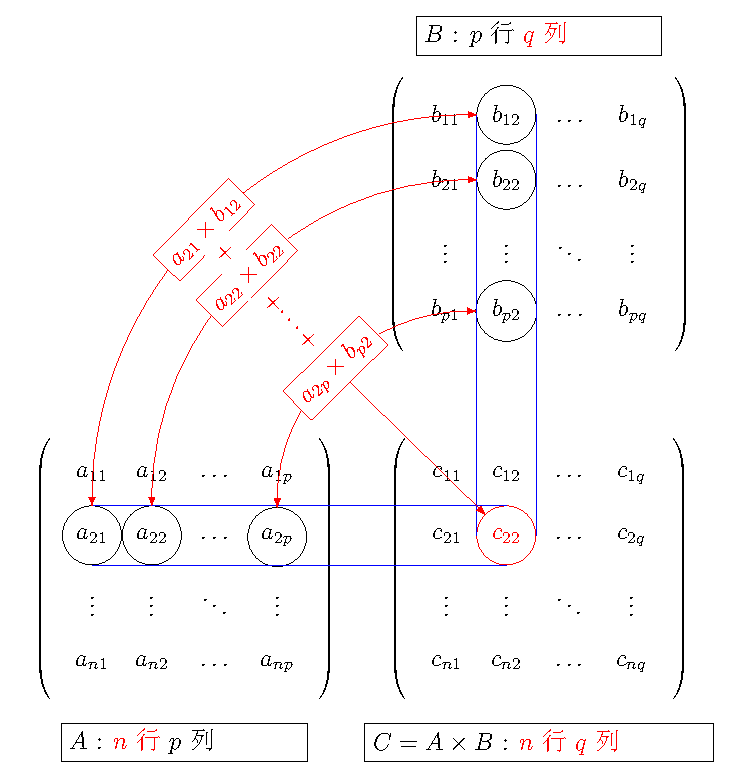
\includegraphics[scale=0.75]{figures/matrix-multiplication.pdf}
    \caption{}
\end{figure}

\begin{definition}[可交换矩阵]
    一般而言, 矩阵的乘法一般不满足交换律, 即 $\vb*{AB}\neq\vb*{BA}$, 若 $\vb*{AB}=\vb*{BA}$, 则称\textit{矩阵} $\vb*{A},~\vb*{B}$ \textit{可交换}.
    可交换的前提是 $\vb*{A},~\vb*{B}$ 至少有一个是单位矩阵.
\end{definition}

\begin{example}
    设 $\vb*{A}=\begin{pmatrix} 1 & 1 \\ 0 & 1 \\\end{pmatrix}$, 求和矩阵 $\vb*{A}$ 可交换的矩阵.
\end{example}
\begin{solution}
    设 $\vb*{X}=\begin{pmatrix} x_1 & x_2 \\ x_3 & x_4 \\\end{pmatrix}$, 有定义得
    $$
    \begin{pmatrix} x_1 & x_2 \\ x_3 & x_4 \\\end{pmatrix}\begin{pmatrix} 1 & 1 \\ 0 & 1 \\\end{pmatrix}=\begin{pmatrix} 1 & 1 \\ 0 & 1 \\\end{pmatrix}\begin{pmatrix} x_1 & x_2 \\ x_3 & x_4 \\\end{pmatrix}\Rightarrow \begin{cases}
        x_1+x_3=x_1\\ 
        x_2+x_4=x_1+x_2\\ 
        x_4=x_3+x_4
    \end{cases}
    $$
    解得 $\begin{cases}
        x_3=0\\ x_1=x_4
    \end{cases}$ 故 $\vb*{X}=\begin{pmatrix} a & b \\ 0 & a \\\end{pmatrix},\forall a,b\in \mathbb{R}.$
\end{solution}

\begin{example}
    设 $\vb*{A}=\begin{pmatrix}
            a_{11} & a_{12} \\
            a_{21} & a_{22} \\
            a_{31} & a_{32} \\
        \end{pmatrix}$,
    $\vb*{B}=\begin{pmatrix}
            b_1 & 0   \\
            0   & b_2
        \end{pmatrix}$,
    $\vb*{C}=\begin{pmatrix}
            c_1 & 0   & 0   \\
            0   & c_2 & 0   \\
            0   & 0   & c_3
        \end{pmatrix}$, 求 $\vb*{AB}$ 和 $\vb*{CA}$.
\end{example}
\begin{solution}
    $\vb*{AB}=\begin{pmatrix}
            a_{11} & a_{12} \\
            a_{21} & a_{22} \\
            a_{31} & a_{32} \\
        \end{pmatrix}\begin{pmatrix}
            b_1 & 0   \\
            0   & b_2
        \end{pmatrix}=\begin{pmatrix}
            a_{11}b_1 & a_{12}b_2 \\
            a_{21}b_1 & a_{22}b_2 \\
            a_{31}b_1 & a_{32}b_2
        \end{pmatrix}$; 同理
    $\vb*{CA}=\begin{pmatrix}
            c_1a_{11} & c_1a_{12} \\
            c_2a_{21} & c_2a_{22} \\
            c_3a_{31} & c_3a_{32}
        \end{pmatrix}$
\end{solution}

\begin{example}
    设 $\vb*{A}$ 是 4 阶方阵, $\vb*{B}$ 是 5 阶方阵, 且 $|\vb*{A}|=2,|\vb*{B}|=-2$, 求 $|-|\vb*{A}|\vb*{B}|$ 与 $|-|\vb*{B}|\vb*{A}|$.
\end{example}
\begin{solution}
    $|-|\vb*{A}|\vb*{B}|=|-2\vb*{B}|=(-2)^{5}|\vb*{B}|=64$, $|-|\vb*{B}|\vb*{A}|=|2\vb*{A}|=2^4|\vb*{A}|=32.$
\end{solution}

\begin{example}
    设 $\vb*{A},~\vb*{B}$ 均为 3 阶矩阵, 满足 $\vb*{AB}+2\vb*{A}+\vb*{B}+\vb*{E}=\vb*{O}$,
    若 $|\vb*{B}|=\mqty|1&2&0\\1&2&0\\1&2&1|$, 求 $|\vb*{A}+\vb*{E}|.$
\end{example}
\begin{solution}
    对 $\vb*{AB}+2\vb*{A}+\vb*{B}+2\vb*{E}$ 使用多项式除法, 得 $$\vb*{AB}+2\vb*{A}+\vb*{B}+2\vb*{E}=(\vb*{A}+\vb*{E})(\vb*{B}+2\vb*{E})=\vb*{E}\Rightarrow|\vb*{A}+\vb*{E}|=\dfrac{1}{|\vb*{B}+2\vb*{E}|}=\dfrac{1}{30}.$$
\end{solution}

\subsection{方阵的幂}

\begin{definition}[方阵的幂]
    对 $ n $ 阶方阵 $ A $, 定义
    $\displaystyle\vb*{A}^{k}=\underbrace{\vb*{A} \cdot \vb*{A} \cdot \cdots \cdot \vb*{A}}_{k \text{个}}$,
    称为 $ \vb*{A} $ 的 $ k $ 次幂.
\end{definition}

\begin{example}
    设 $\vb*{A}=\mqty(\dfrac{2}{3}&-\dfrac{1}{3}&-\dfrac{1}{3}\\[6pt]-\dfrac{1}{3}&\dfrac{2}{3}&-\dfrac{1}{3}\\[6pt]-\dfrac{1}{3}&-\dfrac{1}{3}&\dfrac{2}{3})$, 求 $\vb*{A}^9$.
\end{example}
\begin{solution}
    $\vb*{A}^2=\mqty(\dfrac{2}{3}&-\dfrac{1}{3}&-\dfrac{1}{3}\\[6pt]-\dfrac{1}{3}&\dfrac{2}{3}&-\dfrac{1}{3}\\[6pt]-\dfrac{1}{3}&-\dfrac{1}{3}&\dfrac{2}{3})^{2}=\dfrac{1}{9}\mqty(6&-3&-3\\-3&6&-3\\-3&-3&6)=\vb*{A}$, 因此 $\vb*{A}^9=\vb*{A}\qty(\vb*{A}^2)^4=\vb*{A}\vb*{A}^4=\vb*{A}\qty(\vb*{A}^2)^2=\vb*{A}^2=\vb*{A}.$
\end{solution}

\subsubsection{利用幂零矩阵求解}

\begin{example}
    设 $\vb*{A}=\mqty(0&1&2&3\\0&0&2&3\\0&0&0&3\\0&0&0&0)$, 求解 $\vb*{A}^n.$
\end{example}
\begin{solution}
    因为 $\vb*{A}^4=\vb*{O}$, 并且
    \begin{flalign*}
        \vb*{A}^2=\mqty(0 & 1 & 2 & 3 \\0&0&2&3\\0&0&0&3\\0&0&0&0)\cdot\mqty(0&1&2&3\\0&0&2&3\\0&0&0&3\\0&0&0&0)=\mqty(0&0&2&9\\0&0&0&6\\0&0&0&0\\0&0&0&0)\\
        \vb*{A}^3=\mqty(0 & 0 & 2 & 9 \\0&0&0&6\\0&0&0&0\\0&0&0&0)\cdot \mqty(0&1&2&3\\0&0&2&3\\0&0&0&3\\0&0&0&0)=\mqty(0&0&2&9\\0&0&0&6\\0&0&0&0\\0&0&0&0)
    \end{flalign*}
\end{solution}

\subsubsection{利用方阵的迹求解}

\begin{theorem}[秩一矩阵的幂]
    当 $\vb*{A}$ 为方阵且秩 $\rank\vb*{A}=1$, 则 $\vb*{A}^n=\qty[\tr(\vb*{A})]^{n-1}\vb*{A}$.
\end{theorem}

\begin{example}
    设 $\vb*{A}=\mqty(a&b&c&d\\2a&2b&2c&2d\\3a&3b&3c&3d\\4a&4b&4c&4d)~  (a,b,c,d)$ 不全为 0, 求解 $\vb*{A}^n.$
\end{example}
\begin{solution}
    显然 $\rank\vb*{A}=1$, 则 $$\vb*{A}^n=\qty[\tr(\vb*{A})]^{n-1}\vb*{A}=(a+2b+3c+4d)^{n-1}\vb*{A}.$$
\end{solution}

\begin{example}
    设 $\vb*{A}=\mqty(0&0&1\\0&1&0\\1&0&0)$, 已知矩阵 $\vb*{B}$ 与矩阵 $\vb*{A}$ 相似, 求
    $\rank(\vb*{B}-2\vb*{E})+\rank(\vb*{B}-\vb*{E})$, 及 $(\vb*{A}-\vb*{E})^n$, $n$ 为大于 1 的正整数.
\end{example}
\begin{solution}
    因为 $\vb*{B}\sim\vb*{A}$, 所以
    \begin{flalign*}
        \rank(\vb*{B}-2\vb*{E})+\rank(\vb*{B}-\vb*{E}) & =\rank(\vb*{A}-2\vb*{E})+\rank(\vb*{A}-\vb*{E})=\rank\mqty(-2 & 0 & 1 \\0&-1&0\\1&0&-2)+\rank\mqty(-1&0&1\\0&0&0\\1&0&-1)\\
                                                       & =3+1=4
    \end{flalign*}
    因为 $\rank(\vb*{A}-\vb*{E})=1$, 所以 $(\vb*{A}-\vb*{E})^n=\qty[\tr(\vb*{A}-\vb*{E})\vb*{A}]^{n-1}(\vb*{A}-\vb*{E})=(-2)^{n-1}\mqty(-1&0&1\\0&0&0\\1&0&-1).$
\end{solution}

\subsubsection{利用二项式展开求解}

\begin{theorem}[矩阵的二项式展开]
    $\displaystyle \vb*{E}-\vb*{A}^n=(\vb*{E}-\vb*{A})\qty(\vb*{E}+\sum_{k=1}^{n-1} \vb*{A}^k)$.
\end{theorem}

\begin{example}
    已知 $\vb*{A}^3=\vb*{O}$, 求 $\qty(\vb*{E}+\vb*{A}+\vb*{A}^2)^{-1}$.
\end{example}
\begin{solution}
    因为 $\vb*{E}-\vb*{A}^3=(\vb*{E}-\vb*{A})\qty(\vb*{E}+\vb*{A}+\vb*{A}^2)$, 又 $\vb*{A}^3=\vb*{O}$, 故 $\qty(\vb*{E}+\vb*{A}+\vb*{A}^2)^{-1}=\vb*{E}-\vb*{A}$.
\end{solution}

\begin{example}
    设 $\vb*{A}=\begin{pmatrix}
            1 & 3 \\
            0 & 1
        \end{pmatrix}$, 求 $\vb*{A}^n$.
\end{example}
\begin{solution}
    由 $\vb*{A}=\begin{pmatrix}
            1 & 3 \\
            0 & 1
        \end{pmatrix}=\begin{pmatrix}
            1 & 0 \\
            0 & 1
        \end{pmatrix}+\begin{pmatrix}
            0 & 3 \\
            0 & 0
        \end{pmatrix}=\vb*{E}+\vb*{B}$, 而
    $\displaystyle\vb*{B}^2=\begin{pmatrix}
            0 & 3 \\
            0 & 0
        \end{pmatrix}\begin{pmatrix}
            0 & 3 \\
            0 & 0
        \end{pmatrix}=\mathrm{0}$,
    所以当 $k\geqslant2$ 时, 有 $\vb*{B}^k=\mathrm{0}$,
    而单位矩阵 $\vb*{E}$ 与任意矩阵可换, 由二项式定理, 得
    \begin{flalign*}
        \vb*{A}^n & =(\vb*{E}+\vb*{B})^n=\sum_{k=0}^{n}\mathrm{C}_n^k\vb*{E}^{n-k}\vb*{B}^k=\vb*{E}^n+\mathrm{C}_n^1\vb*{E}^{n-1}B \\
                  & =\begin{pmatrix}
                         1 & 0 \\
                         0 & 1
                     \end{pmatrix}+n\begin{pmatrix}
                                        1 & 0 \\
                                        0 & 1
                                    \end{pmatrix}\begin{pmatrix}
                                                     0 & 3 \\
                                                     0 & 0
                                                 \end{pmatrix}=\begin{pmatrix}
                                                                   1 & 3n \\
                                                                   0 & 1
                                                               \end{pmatrix}.
    \end{flalign*}
\end{solution}

\begin{example}[2002 复旦大学]
    证明: $$\begin{pmatrix}
            \dfrac{3}{2} & -\dfrac{1}{2} \\[6pt]
            \dfrac{1}{2} & \dfrac{1}{2}
        \end{pmatrix}^{100}=\begin{pmatrix}
            51 & -50 \\
            50 & -49
        \end{pmatrix}.$$
\end{example}
\begin{proof}[{\songti \textbf{证}}]
    注意到 \begin{flalign*}
        \begin{pmatrix}
            \dfrac{3}{2} & -\dfrac{1}{2} \\[6pt]
            \dfrac{1}{2} & \dfrac{1}{2}
        \end{pmatrix}=\begin{pmatrix}
                          1 & 0 \\
                          0 & 1
                      \end{pmatrix}+\begin{pmatrix}
                                        \dfrac{1}{2} & -\dfrac{1}{2} \\[6pt]
                                        \dfrac{1}{2} & -\dfrac{1}{2}
                                    \end{pmatrix}=\begin{pmatrix}
                                                      1 & 0 \\
                                                      0 & 1
                                                  \end{pmatrix}+\begin{pmatrix}
                                                                    \dfrac{1}{2} \\[6pt]
                                                                    \dfrac{1}{2}
                                                                \end{pmatrix}(1,-1) =\vb*{E}+\vb*{\alpha}\vb*{\beta}^{\top}
    \end{flalign*}
    其中 $\vb*{E}$ 是二阶单位矩阵, $\vb*{\alpha}=\qty(\dfrac{1}{2},\dfrac{1}{2})^{\top}$, $\vb*{\beta}=(1,-1)^{\top}$, 并且 $\vb*{\beta}\vb*{\alpha}^T=0$, 所以
    $$\qty(\vb*{\alpha\beta}^\top)^2=\qty(\vb*{\alpha\beta}^{\top})\qty(\vb*{\alpha\beta}^{\top})=\vb*{\alpha}\qty(\vb*{\beta}^{\top}\vb*{\alpha})\vb*{\beta}^{\top}=\vb*{O}$$
    于是 \begin{flalign*}
        \begin{pmatrix}
            \dfrac{3}{2} & -\dfrac{1}{2} \\[6pt]
            \dfrac{1}{2} & \dfrac{1}{2}
        \end{pmatrix}^{100} & =\qty(\vb*{E}+\vb*{\alpha}\vb*{\beta}^{\top})^{100}=\sum_{k=0}^{100}\mathrm{C}_{100}^k\qty(\vb*{\alpha\beta}^\top)^k=\vb*{E}+100\vb*{\alpha\beta}^{\top} \\
                                             & =\begin{pmatrix}
                                                    1 & 0 \\
                                                    0 & 1
                                                \end{pmatrix}+100\begin{pmatrix}
                                                                     1 \\1
                                                                 \end{pmatrix}(1,-1)=\begin{pmatrix}
                                                                                         51 & -50 \\
                                                                                         50 & -49
                                                                                     \end{pmatrix}.
    \end{flalign*}
\end{proof}

\subsection{分块矩阵}

\begin{theorem}[分块矩阵的加减法]
    若矩阵 $ \vb*{A} $ 与矩阵 $ \vb*{B} $ 有相同的行数和列数, 且有
    $$\vb*{A}=\mqty(\vb*{A}_{11} & \cdots & \vb*{A}_{1 r} \\
        \vdots & & \vdots \\
        \vb*{A}_{s 1} & \cdots & \vb*{A}_{s r})
        , \quad \vb*{B}=\mqty(\vb*{B}_{11} & \cdots & \vb*{B}_{1 r} \\
        \vdots & & \vdots \\
        \vb*{B}_{s 1} & \cdots & \vb*{B}_{s r})$$
    其中 $ \vb*{A}_{i j} $ 与 $ \vb*{B}_{i j} $ 有相同的行数和列数, 则
    $$\vb*{A} \pm \vb*{B}=\mqty(\vb*{A}_{11} \pm \vb*{B}_{11}   & \cdots & \vb*{A}_{1 r} \pm \vb*{B}_{1 r} \\
        \vdots                                        &        & \vdots                                        \\
        \vb*{A}_{s 1} \pm \vb*{B}_{s 1} & \cdots & \vb*{A}_{s r} \pm \vb*{B}_{s r}).$$
\end{theorem}

\begin{theorem}[分块矩阵的数乘]
    设矩阵 $ \vb*{A}=\mqty(\vb*{A}_{11} & \cdots & \vb*{A}_{1 r} \\ \vdots & & \vdots \\ \vb*{A}_{s 1} & \cdots & \vb*{A}_{s r})$, $\lambda $ 为数, 则
    $$\lambda  \vb*{A}=\mqty(\lambda  \vb*{A}_{11} & \cdots & \lambda  \vb*{A}_{1 r} \\
        \vdots & & \vdots \\
        \lambda  \vb*{A}_{s 1} & \cdots & \lambda  \vb*{A}_{s r}).$$
\end{theorem}

\begin{theorem}[分块矩阵的乘法]
    若 $ \vb*{A} $ 为 $ m \times l $ 矩阵, $ \vb*{B} $ 为 $ l \times n $ 矩阵, 且
    $$\vb*{A}=\mqty(\vb*{A}_{11}  & \cdots & \vb*{A}_{1 t} \\
        \vdots        &        & \vdots        \\
        \vb*{A}_{s 1} & \cdots & \vb*{A}_{s t})
        , \quad \vb*{B}=\mqty(\vb*{B}_{11}  & \cdots & \vb*{B}_{1 r} \\
        \vdots        &        & \vdots        \\
        \vb*{B}_{t 1} & \cdots & \vb*{B}_{t r})$$
    其中 $ \vb*{A}_{i 1}, \vb*{A}_{i 2}, \cdots, \vb*{A}_{i i} $ 的列数分别与 $ \vb*{B}_{1 j}, \vb*{B}_{2 j}, \cdots, \vb*{B}_{i j} $ 的行数相等, 则
    $$\vb*{A B}=\mqty(\vb*{C}_{11}  & \cdots & \vb*{C}_{1 r} \\
        \vdots  &        & \vdots  \\
        \vb*{C}_{s 1} & \cdots & \vb*{C}_{s r})$$
    其中 $ \vb*{C}_{i j}=\displaystyle \sum_{k=1}^{t} \vb*{A}_{i k} \vb*{B}_{k j}(i=1, \cdots, s ; j=1, \cdots, r) $.
\end{theorem}

\begin{theorem}[分块矩阵的转置]
    设矩阵 $ \vb*{A}=\mqty(\vb*{A}_{11} & \cdots & \vb*{A}_{1 r} \\ \vdots & & \vdots \\ \vb*{A}_{s 1} & \cdots & \vb*{A}_{s r})
    $, 则 $ \vb*{A}^{\top}=\mqty(\vb*{A}_{11}^{\top} & \cdots & \vb*{A}_{s 1}^{\top} \\ \vdots & & \vdots \\ \vb*{A}_{1 r}^{\top} & \cdots & \vb*{A}_{s r}^{\top}) $.
\end{theorem}

\begin{theorem}[分块矩阵的行列式]
    设 $ \vb*{A}=\left(\begin{array}{llll}\vb*{A}_{1} & & & \\ & \vb*{A}_{2} & & \\ & & \ddots & \\ & & & A_{m}\end{array}\right) $, 其中 $ \vb*{A}_{i}(i=1,2, \cdots, m) $ 都是方阵, 则
          $$|\vb*{A}|=\left|\vb*{A}_{1}\right|\left|\vb*{A}_{2}\right| \cdots\left|\vb*{A}_{m}\right|, \quad \vb*{A}^{n}=\left(\begin{array}{llll}
                      \vb*{A}_{1}^{n} &                 &        &                 \\
                                      & \vb*{A}_{2}^{n} &        &                 \\
                                      &                 & \ddots &                 \\
                                      &                 &        & \vb*{A}_{m}^{n}
                  \end{array}\right) .$$
\end{theorem}

\subsection{Carlson 不等式及其应用}

\begin{theorem}[Carlson 不等式]
    在 $n\times m$ 的非负实数矩阵中, $m$ 列每列元素之和的几何平均值不小于矩阵中 $n$ 行每行元素的几何平均值之和. 即对于 $n\times m$ 矩阵
    $$\begin{pmatrix}
            a_{11} & a_{12} & \dots  & a_{1m} \\
            a_{21} & a_{22} & \dots  & a_{2m} \\
            \vdots & \vdots & \ddots & \vdots \\
            a_{n1} & a_{n2} & \dots  & a_{nm} \\
        \end{pmatrix}$$
    其中 $a_{ij}\geqslant0~ (i=1,2,\cdots,n,j=1,2,\cdots,m)$, 则
    $$\qty[\prod_{j=1}^{m}\qty(\sum_{i=1}^{n}a_{ij})]^{\frac{1}{m}}\geqslant \sum_{i=1}^{n}\qty(\prod_{j=1}^{m}a_{ij})^{\frac{1}{m}}$$
    其中, 等号成立的充要条件是至少有一列数都是 0 或所有行中的数对应成比例.
\end{theorem}
\begin{proof}[{\songti \textbf{证}}]
    记 $\displaystyle A_j = \sum_{i=1}^{n}a_{ij}~ (j=1,2,\cdots,m),~G_j=\prod_{j=1}^{m}a_{ij}~ (i=1,2,\cdots,n)$, 
    若某个 $A_j=0$, 则由 $a_{ij}\geqslant 0~ (i=1,2,\cdots,n)$, 得 $$a_{1j}=a_{2j}=\cdots=a_{nj}=0$$
    此时, $G_1=G_2=\cdots=G_n=0$, 从而 $$\qty[\prod_{j=1}^{m}\qty(\sum_{i=1}^{n}a_{ij})]^{\frac{1}{m}}=\sum_{i=1}^{n}\qty(\prod_{j=1}^{m}a_{ij})^{\frac{1}{m}}$$
    若所有 $A_j>0$, 由均值不等式得 $$\dfrac{a_{i1}}{A_1}+\dfrac{a_{i2}}{A_2}+\cdots+\dfrac{a_{im}}{A_m}\geqslant m\qty(\dfrac{\displaystyle\prod_{j=1}^{m}a_{ij}}{\displaystyle\prod_{j=1}^{m}A_j})^{\frac{1}{m}}~ (i=1,2,\cdots,n)$$
    将以上 $n$ 个不等式相加得
    $$m\geqslant m\sum_{i=1}^{n}\qty(\dfrac{\displaystyle\prod_{j=1}^{m}a_{ij}}{\displaystyle\prod_{j=1}^{m}A_j})^{\frac{1}{m}}=m\dfrac{\displaystyle\sum_{i=1}^{n}G_i^{\frac{1}{m}}}{\qty(\displaystyle\prod_{j=1}^{m}A_j)^{\frac{1}{m}}}$$
    等号成立的充要条件是至少有一列数都是 0 或 $\dfrac{a_{i1}}{A_1}=\dfrac{a_{i2}}{A_2}=\cdots=\dfrac{a_{im}}{A_m}$.
\end{proof}

\begin{example}
    已知 $a,b,c>0$, 证明: $$\qty(a^2+ab+b^2)\qty(b^2+bc+c^2)\qty(c^2+ca+a^2)\geqslant (ab+bc+ca)^3.$$
\end{example}
\begin{proof}[{\songti \textbf{证}}]
    构造 $3\times 3$ 矩阵
    $$\begin{pmatrix}
            a^2 & c^2 & ca  \\
            ab  & b^2 & a^2 \\
            b^2 & bc  & c^2
        \end{pmatrix}$$
    由 Carlson 不等式得证.
\end{proof}

\begin{example}
    已知 $a,b,c>0$, $a^2+b^2+c^2=14$, 求证: $a^5+\dfrac{b^5}{8}+\dfrac{c^5}{27}\geqslant 14.$
\end{example}
\begin{proof}[{\songti \textbf{证}}]
    构造 $3\times 5$ 矩阵
    $$\begin{pmatrix}
            a^5             & a^5             & 1 & 1 & 1 \\[6pt]
            \dfrac{b^5}{8}  & \dfrac{b^5}{8}  & 4 & 4 & 4 \\[6pt]
            \dfrac{c^5}{27} & \dfrac{c^5}{27} & 9 & 9 & 9
        \end{pmatrix}$$
    由 Carlson 不等式得, 
    \begin{flalign*}
        \qty[\qty(a^5+\dfrac{b^5}{8}+\dfrac{c^5}{27})^2(1+4+9)^3]^{\frac{1}{5}} & \geqslant \qty(a^5\cdot a^5\cdot 1^3)^{\frac{1}{5}}+\qty(\dfrac{b^5}{8}\cdot \dfrac{b^5}{8}\cdot 4^3)^{\frac{1}{5}}+\qty(\dfrac{c^5}{27}\cdot\dfrac{c^5}{27}\cdot 9^3)^{\frac{1}{5}} \\
        \qty[\qty(a^5+\dfrac{b^5}{8}+\dfrac{c^5}{27})^214^3]^{\frac{1}{5}}      & \geqslant a^2+b^2+c^2=14
    \end{flalign*}
    整理得证 $a^5+\dfrac{b^5}{8}+\dfrac{c^5}{27}\geqslant 14.$
\end{proof}

\begin{example}
    已知 $a_i>0~ (i=1,2,\cdots,n),~n\geqslant 2$, 且 $\displaystyle\sum_{i=1}^{n}a_i=1$, 
    证明: $\displaystyle\sum_{i=1}^{n}\dfrac{a_i}{2-a_i}\geqslant \dfrac{n}{2n-1}.$
\end{example}
\begin{proof}[{\songti \textbf{证}}]
    原不等式等价为 $$\sum_{i=1}^{n}\dfrac{2}{2-a_i}\geqslant \dfrac{2n^2}{2n-1}$$
    为此, 构造 $n\times 2$ 矩阵
    $$\begin{pmatrix}
            \dfrac{2}{2-a_1} & 2-a_1  \\[6pt]
            \dfrac{2}{2-a_2} & 2-a_2  \\[6pt]
            \vdots           & \vdots \\[6pt]
            \dfrac{2}{2-a_n} & 2-a_n
        \end{pmatrix}$$
    由 Carlson 不等式得, 
    \begin{flalign*}
        \qty[\qty(\sum_{i=1}^{n}\dfrac{2}{2-a_i})\sum_{i=1}^{n}(2-a_i)]^{\frac{1}{2}}\geqslant \sqrt{2}n\Rightarrow\qty(\sum_{i=1}^{n}\dfrac{2}{2-a_i})(2n-1)\geqslant 2n^2
    \end{flalign*}
    整理得证 $\displaystyle\sum_{i=1}^{n}\dfrac{a_i}{2-a_i}\geqslant \dfrac{n}{2n-1}.$
\end{proof}

\begin{example}
    (第 36 届 IMO) 设 $a,b,c>0$, 且 $abc=1$, 证明: $\dfrac{1}{a^3(b+c)}+\dfrac{1}{b^3(c+a)}+\dfrac{1}{c^3(a+b)}\geqslant\dfrac{3}{2}.$
\end{example}
\begin{proof}[{\songti \textbf{证}}]
    原不等式等价为 $$\dfrac{b^2c^2}{a(b+c)}+\dfrac{a^2c^2}{b(c+a)}+\dfrac{a^2b^2}{c(a+b)}$$
    构造 $3\times 2$ 矩阵
    $$\begin{pmatrix}
            \dfrac{b^2c^2}{a(b+c)} & a(b+c) \\[6pt]
            \dfrac{a^2c^2}{b(a+c)} & b(a+c) \\[6pt]
            \dfrac{a^2b^2}{c(a+b)} & c(a+b)
        \end{pmatrix}$$
    由 Carlson 不等式得, 
    \begin{flalign*}
        \qty{\qty[\dfrac{b^2c^2}{a(b+c)}+\dfrac{a^2c^2}{b(c+a)}+\dfrac{a^2b^2}{c(a+b)}]\cdot2(ab+bc+ca)}^{\frac{1}{2}} & \geqslant ab+bc+ca                                                                      \\
        \dfrac{b^2c^2}{a(b+c)}+\dfrac{a^2c^2}{b(c+a)}+\dfrac{a^2b^2}{c(a+b)}                                           & \geqslant \dfrac{1}{2}(ab+bc+ca)\geqslant \dfrac{3}{2}\sqrt[3]{a^2b^2c^2}=\dfrac{3}{2}.
    \end{flalign*}
\end{proof}
\section{伴随矩阵与逆矩阵}

\subsection{伴随矩阵}

\begin{definition}[伴随矩阵]
    设 $ \boldsymbol{A}=\left(a_{i j}\right) $ 是 $ n $ 阶方阵 $ (n \geqslant 2)$,$A $ 的伴随矩阵 $\vb*{A}^*$ (或 $\adj\vb*{A}$) 定义为
    $$\boldsymbol{A}^{*}=\begin{pmatrix}
            A_{11}  & A_{21}  & \cdots & A_{n 1} \\
            A_{12}  & A_{22}  & \cdots & A_{n 2} \\
            \vdots  & \vdots  &        & \vdots  \\
            A_{1 n} & A_{2 n} & \cdots & A_{n n}
        \end{pmatrix},$$
    其中 $ A_{i j} $ 为 $ \boldsymbol{A} $ 的元素 $ a_{i j}~ (i, j=1,2, \cdots, n) $ 的代数余子式.
\end{definition}
伴随矩阵具有如下性质:
\setcounter{magicrownumbers}{0}
\begin{table}[H]
    \centering
    \begin{tabular}{l l}
        (\rownumber) $\displaystyle \boldsymbol{AA}^{*}=\boldsymbol{A}^{*} \boldsymbol{A}=|\boldsymbol{A}| \boldsymbol{E}$                                            & (\rownumber) $\displaystyle(\lambda \boldsymbol{A})^{*}=\lambda^{n-1} \boldsymbol{A}^{*}$                                                                                                                                                            \\
        (\rownumber) $\displaystyle \left|\boldsymbol{A}^{*}\right|=|\boldsymbol{A}|^{n-1} $                                                                          & (\rownumber) $\displaystyle\left(\boldsymbol{A}^{*}\right)^{\top}=\left(\boldsymbol{A}^{\top}\right)^{*}$                                                                                                                                            \\
        \midrule
        (\rownumber) $\displaystyle(\boldsymbol{AB})^{*}=\boldsymbol{B}^{*} \boldsymbol{A}^{*}$                                                                       & (\rownumber) $\displaystyle\text{当 } \boldsymbol{A} \text{ 可逆时,} \boldsymbol{A}^{*}=|\boldsymbol{A}| \boldsymbol{A}^{-1}$                                                                                                                       \\
        (\rownumber) $\displaystyle\text{当 } \boldsymbol{A} \text{ 可逆时,}\left(\boldsymbol{A}^{*}\right)^{-1}=\frac{1}{|\boldsymbol{A}|} \boldsymbol{A}$          & (\rownumber) $\displaystyle\text{当 } \boldsymbol{A} \text{ 可逆时,}\left(\boldsymbol{A}^{*}\right)^{-1}=\left(\boldsymbol{A}^{-1}\right)^{*} $                                                                                                     \\
        \midrule
        (\rownumber) $\displaystyle\left(\boldsymbol{A}^{*}\right)^{*}=\begin{cases}|\boldsymbol{A}|^{n-2} \boldsymbol{A}, & n>2 \\ \boldsymbol{A}, & n=2\end{cases}$ & (\rownumber) $\displaystyle\operatorname{rank} \boldsymbol{A}^{*}=\left\{\begin{array}{ll}n, & \operatorname{rank} \boldsymbol{A}=n \\ 1, & \operatorname{rank} \boldsymbol{A}=n-1 \\ 0, & \operatorname{rank} \boldsymbol{A}<n-1\end{array}\right.$ \\
    \end{tabular}
\end{table}

\begin{example}
    设矩阵 $\vb*{A}=\mqty(2&1&0\\1&2&0\\0&0&1)$,矩阵 $\vb*{B}$ 满足 $\vb*{ABA}^*=2\vb*{BA}^*+\vb*{E}$,求 $\qty|2\vb*{B}^\top|.$
\end{example}
\begin{solution}
    注意到 $\det\vb*{A}=3$,且 $\vb*{A}^*\vb*{A}=|\vb*{A}|\vb*{E}$,对 $\vb*{ABA}^*=2\vb*{BA}^*+\vb*{E}$,右乘矩阵 $\vb*{A}$,得 
    $$3\vb*{AB}=6\vb*{B}+\vb*{A}\Rightarrow 3(\vb*{A}-2\vb*{E})\vb*{B}=\vb*{A}\Rightarrow |3(\vb*{A}-2\vb*{E})\vb*{B}|=3\Rightarrow |\vb*{B}|=\dfrac{1}{9|\vb*{A}-2\vb*{E}|}$$
    其中 $|\vb*{A}-2\vb*{E}|=\mqty|0&1&0\\1&0&0\\0&0&-1|=1$,于是 $\vb*{B}=\dfrac{1}{9}\Rightarrow \qty|2\vb*{B}^\top|=\dfrac{8}{9}.$
\end{solution}

\begin{example}
    求矩阵 $\vb*{A}=\mqty(0&0&0&1&3\\0&0&0&-1&2\\1&1&1&0&0\\0&1&1&0&0\\0&0&1&0&0)$ 的所有代数余子式之和.
\end{example}
\begin{solution}
    记矩阵分块矩阵 $\vb*{A}=\mqty(\vb*{O}_{2\times 3}&\vb*{B}\\\vb*{C}&\vb*{O}_{3\times 2})$,其中 $\vb*{B}=\mqty(1&3\\-1&2),~\vb*{C}=\mqty(1&1&1\\0&1&1\\0&0&1)$,则 $\det\vb*{B}=5,~\det\vb*{C}=1$,那么
    $$\vb*{A}^*=|\vb*{A}|\vb*{A}^{-1}=(-1)^{2\times 3}|\vb*{B}|~|\vb*{C}|\mqty(\vb*{O}_{3\times 2}&\vb*{C}^{-1}\\\vb*{B}^{-1}&\vb*{O}_{2\times 3})=\mqty(0&0&5&-5&0\\0&0&0&5&-5\\0&0&0&0&5\\2&-3&0&0&0\\1&1&0&0&0)$$
    因此矩阵 $\vb*{A}$ 的所有代数余子式之和为 $5-5+5-5+5+2-3+1+1=6.$
\end{solution}

\subsection{可逆矩阵}
可逆矩阵具有如下性质:
\begin{enumerate}[label=(\arabic{*})]
    \item 方阵 $ \boldsymbol{A} $ 可逆的充分必要条件是 $ |\boldsymbol{A}| \neq 0 $;
    \item 若 $ \boldsymbol{A} $ 可逆,则 $ \boldsymbol{A}^{\top} $ 亦可逆,
          且 $ \left(\boldsymbol{A}^{\top}\right)^{-1}=\left(\boldsymbol{A}^{-1}\right)^{\top}$ ;
    \item 若 $ \boldsymbol{A} $ 可逆,则 $ \boldsymbol{A}^{-1} $ 亦可逆,且 $ \left(\boldsymbol{A}^{-1}\right)^{-1}=\boldsymbol{A} $;
    \item 若 $ \boldsymbol{A} $ 可逆,数 $ \lambda \neq 0 $,则 $ \lambda \boldsymbol{A} $ 亦可逆,且 $ (\lambda \boldsymbol{A})^{-1}=\dfrac{1}{\lambda} \boldsymbol{A}^{-1}$ ;
    \item 若 $\boldsymbol{A}$ 可逆,则 $\left|\boldsymbol{A}^{-1}\right|=|\boldsymbol{A}|^{-1}$;
    \item 若 $\boldsymbol{A},\boldsymbol{B}$ 为同阶方阵,且均可逆,则 $\boldsymbol{AB}$ 亦可逆,且 $(\boldsymbol{AB})^{-1}=\boldsymbol{B}^{-1}\boldsymbol{A}^{-1}.$
\end{enumerate}

\begin{theorem}[矩阵逆的和]
    设矩阵 $\vb*{A}$ 与 $\vb*{B}$ 均为 $n$ 阶矩阵,则 $\qty|\vb*{A}^{-1}+\vb*{B}^{-1}|=\dfrac{|\vb*{A}+\vb*{B}|}{|\vb*{A}|\cdot|\vb*{B}|}.$
\end{theorem}
\begin{proof}[{\songti \textbf{证}}]
    $\qty|\vb*{A}^{-1}+\vb*{B}^{-1}|=\qty|\vb*{EA}^{-1}+\vb*{B}^{-1}\vb*{E}|=\qty|\vb*{B}^{-1}\vb*{BA}^{-1}+\vb*{B}^{-1}\vb*{AA}^{-1}|=\qty|\vb*{B}^{-1}(\vb*{B}+\vb*{A})\vb*{A}^{-1}|=\dfrac{|\vb*{A}+\vb*{B}|}{|\vb*{A}|\cdot|\vb*{B}|}.$
\end{proof}

\begin{theorem}[分块矩阵的逆]
    设 $\vb*{A}$ 是 $m\times m$ 可逆矩阵,$\vb*{B}$ 是 $m\times n$ 矩阵,$\vb*{C}$ 是 $n\times m$ 矩阵,$\vb*{D}$ 是 $n\times n$ 可逆矩阵,则有以下分块矩阵的求逆公式:
    $$\mqty(\vb*{A}&\vb*{B}\\\vb*{C}&\vb*{D})^{-1}=\mqty(\vb*{A}^{-1}+\vb*{A}^{-1}\vb*{BWCA}^{-1}&-\vb*{A}^{-1}\vb*{BW}\\-\vb*{WCA}^{-1}&\vb*{W})$$
    其中 $\vb*{W}=\qty(\vb*{D}-\vb*{CA}^{-1}\vb*{B})^{-1}.$
\end{theorem}
\begin{proof}[{\songti \textbf{证}}]
    为方便叙述,记 $\vb*{W}=\qty(\vb*{D}-\vb*{CA}^{-1}\vb*{B})^{-1}$ 设 $\vb*{F}=\mqty(\vb*{A}&\vb*{B}\\\vb*{C}&\vb*{D})$ 的逆矩阵为 $\vb*{U}=\mqty(\vb*{U}_{11}&\vb*{U}_{12}\\\vb*{U}_{21}&\vb*{U}_{22})$,其中 $\vb*{U}$ 的分块与 $\mqty(\vb*{A}&\vb*{B}\\\vb*{C}&\vb*{D})$ 分块后满足乘法原则,
    则根据可逆矩阵的定义 $\vb*{FU}=\vb*{E}$,下面直接计算 $\vb*{FU}$ 的分块矩阵的乘积即可,
    \begin{flalign*}
        \mqty(\vb*{E}_{11} & \vb*{O} \\\vb*{O}&\vb*{E}_{12})=\vb*{E}=\vb*{FU}=\mqty(\vb*{A}&\vb*{B}\\\vb*{C}&\vb*{D})\mqty(\vb*{U}_{11}&\vb*{U}_{12}\\\vb*{U}_{21}&\vb*{U}_{22})=\mqty(\vb*{AU}_{11}+\vb*{BU}_{21}&\vb*{AU}_{12}+\vb*{BU}_{22}\\\vb*{CU}_{11}+\vb*{DU}_{21}&\vb*{CU}_{12}+\vb*{DU}_{22})
    \end{flalign*}
    所以,各个矩阵小块分别对应相等得:
    \begin{equation}
        \vb*{AU}_{11}+\vb*{BU}_{21}=\vb*{E}_{11}
        \tag*{(1)}
    \end{equation}
    \begin{equation}
        \vb*{AU}_{12}+\vb*{BU}_{22}=\vb*{O}
        \tag*{(2)}
    \end{equation}
    \begin{equation}
        \vb*{CU}_{11}+\vb*{DU}_{21}=\vb*{O}
        \tag*{(3)}
    \end{equation}
    \begin{equation}
        \vb*{CU}_{12}+\vb*{DU}_{22}=\vb*{E}_{22}
        \tag*{(4)}
    \end{equation}
    由 (1) 可得: $\vb*{U}_{11}=\vb*{A}^{-1}(\vb*{E}_{11}-\vb*{BU}_{21})$,代入 (3) 中,有
    $$\vb*{CA}^{-1}(\vb*{E}_{11}-\vb*{BU}_{21})+\vb*{DU}_{21}=\vb*{O}$$
    化简后得: $\vb*{CA}^{-1}+\qty(\vb*{D}-\vb*{CA}^{-1}\vb*{B})\vb*{U}_{21}=\vb*{O}$,即
    $$\vb*{U}_{21}=-\qty(\vb*{D}-\vb*{CA}^{-1}\vb*{B})\vb*{CA}^{-1}=-\vb*{WCA}^{-1}$$
    由 (4) 可得: $\vb*{U}_{12}=\vb*{C}^{-1}(\vb*{E}_{22}-\vb*{DU}_{22})$,代入 (2) 中,有
    $$\vb*{A}\qty(\vb*{C}^{-1}-\vb*{C}^{-1}\vb*{DU}_{22})+\vb*{BU}_{22}=\vb*{O}$$
    即
    \begin{flalign*}
        \vb*{U}_{22} & =-\qty(\vb*{B}-\vb*{AC}^{-1}\vb*{D})^{-1}\vb*{AC}^{-1}=-\qty(\vb*{B}-\vb*{AC}^{-1}\vb*{D})^{-1}\qty(\vb*{CA}^{-1})^{-1}=-\qty(\qty(\vb*{CA}^{-1})\qty(\vb*{B}-\vb*{AC}^{-1}\vb*{D}))^{-1} \\
                     & =-\qty(\vb*{CA}^{-1}\vb*{B}-\vb*{CA}^{-1}\vb*{AC}^{-1}\vb*{D})^{-1}=-\qty(\vb*{CA}^{-1}\vb*{B}-\vb*{D})^{-1}=\qty(\vb*{D}-\vb*{CA}^{-1}\vb*{B})=\vb*{W}
    \end{flalign*}
    由 (2) 可得: $\vb*{U}_{12}=-\vb*{A}^{-1}\vb*{BU}_{22}$ 将 $\vb*{U}_{22}=\vb*{W}$ 代入其中可得: $\vb*{U}_{12}=-\vb*{A}^{-1}\vb*{BW}$,由 (3) 可得: 
    $\vb*{U}_{11}=\vb*{A}^{-1}(\vb*{E}_{11}-\vb*{BU}_{21})$,将 $\vb*{U}_{21}=-\vb*{WCA}^{-1}$ 代入其中可得:
    $$\vb*{U}_{11}=\vb*{A}^{-1}\qty(\vb*{E}_{11}+\vb*{BWCA}^{-1})=\vb*{A}^{-1}+\vb*{A}^{-1}\vb*{BWCA}^{-1}$$
    综上所述,即得证.
\end{proof}

% \begin{example}
%     设 5 阶矩阵 $\vb*{A}=\begin{pmatrix}
%             1 & 1 & 0 & 0   & 0   \\
%             1 & 3 & 0 & 0   & 0   \\
%             0 & a & a & a^2 & a^3 \\
%             a & 1 & 0 & a   & a^2 \\
%             0 & a & 0 & 0   & a
%         \end{pmatrix}$,求使得 $\vb*{A}$ 可逆的 $a$ 值,并计算 $\vb*{A}^{-1}.$
% \end{example}
% \begin{solution}
%     对行列式 $|\vb*{A}|$ 进行初等变换,令 $|\vb*{A}|\neq0$ 即可,
%     \begin{flalign*}
%         |\vb*{A}|&=\begin{vmatrix}
%                       1 & 1 & 0 & 0   & 0   \\
%                       1 & 3 & 0 & 0   & 0   \\
%                       0 & a & a & a^2 & a^3 \\
%                       a & 1 & 0 & a   & a^2 \\
%                       0 & a & 0 & 0   & a
%                   \end{vmatrix}\xlongequal[]{c_2-c_1}
%         \begin{vmatrix}
%             1 & 0   & 0 & 0   & 0   \\
%             1 & 2   & 0 & 0   & 0   \\
%             0 & a   & a & a^2 & a^3 \\
%             a & 1-a & 0 & a   & a^2 \\
%             0 & a   & 0 & 0   & a
%         \end{vmatrix}\\
%         &=\left|\begin{array}{c:cccc}
%             1 & 0 & 0 & 0 & 0\\ \hdashline 
%             1 & 2 & 0 & 0 & 0\\
%             0 & a & a & a^2 & a^3\\
%             a & 1-a & 0 & a & a^2\\
%             0 & a & 0 & 0 &a
%            \end{array}\right|=
%            \left|\begin{array}{c:ccc}
%             2 & 0 & 0 & 0\\ \hdashline 
%             a & a & a^2 & a^3\\
%             1-a & 0 & a & a^2\\
%             a & 0 & 0 &a
%            \end{array}\right|=2a^3\neq 0
%     \end{flalign*}
%     则 $a\neq0$ 时,矩阵 $\vb*{A}$ 可逆,且 
%     \begin{flalign*}
%         \vb*{A}^{-1}=\dfrac{1}{|\vb*{A}|}\vb*{A}^*=
%     \end{flalign*}
% \end{solution}

\begin{example}
    求矩阵 $\vb*{A}=\mqty(2&3&5\\1&2&7\\3&4&4)$ 的逆矩阵.
\end{example}
\begin{solution}
    \textbf{法一: }因为 $\vb*{A}^{-1}=\dfrac{1}{|\vb*{A}|}\vb*{A}^*$,于是
    \begin{flalign*}
        \vb*{A}^{-1}=\dfrac{1}{\mqty|2 & 3 & 5 \\1&2&7\\3&4&4|}\mqty(\mqty|2&7\\4&4|&-\mqty|3&5\\4&4|&\mqty|3&5\\2&7|\\
        -\mqty|1                       & 7     \\4&4|&\mqty|2&5\\3&4|&-\mqty|2&5\\1&7|\\ \mqty|1&2\\3&4|&-\mqty|2&3\\3&4|&\mqty|2&3\\1&2|)=\mqty(-20&8&11\\17&-7&-9\\-2&1&1).
    \end{flalign*}
    \textbf{法二: }将 $\begin{pNiceArray}{c:c}
            \vb*{A} & \vb*{E}
        \end{pNiceArray}$ 初等行变换为 $\begin{pNiceArray}{c:c}
            \vb*{E} & \vb*{B}
        \end{pNiceArray}$,则 $\vb*{B}=\vb*{A}^{-1}$,于是
    \begin{flalign*}
        \begin{pNiceArray}{c:c}
            \vb*{A} & \vb*{E}
        \end{pNiceArray} & =\begin{pNiceArray}{ccc:ccc}
                                2 & 3 & 5 & 1 & 0 & 0 \\
                                1 & 2 & 7 & 0 & 1 & 0 \\
                                3 & 4 & 4 & 0 & 0 & 1 \\
                            \end{pNiceArray}\xrightarrow[r_3-3r_1]{\substack{r_1\leftrightarrow r_2 \\r_2-2r_1}}\begin{pNiceArray}{ccc:ccc}
            1 & 2  & 7   & 0 & 1  & 0 \\
            0 & -1 & -9  & 1 & -2 & 0 \\
            0 & -2 & -17 & 0 & -3 & 1 \\
        \end{pNiceArray}\\
                                & \xrightarrow[r_3+2r_2]{\substack{r_1+r_3                          \\r_2\times(-1)}}\begin{pNiceArray}{ccc:ccc}
            1 & 0 & -10 & 0  & -2 & 1 \\
            0 & 1 & 9   & -1 & 2  & 0 \\
            0 & 0 & 1   & -2 & 1  & 1 \\
        \end{pNiceArray}\xrightarrow[r_2-9r_3]{r_1+10r_3}    \begin{pNiceArray}{ccc:ccc}
            1 & 0 & 0 & -20 & 8  & 11 \\
            0 & 1 & 0 & 17  & -7 & -9 \\
            0 & 0 & 1 & -2  & 1  & 1  \\
        \end{pNiceArray}
    \end{flalign*}
    于是 $\vb*{A}^{-1}=\mqty(-20  & 8  & 11 \\17  & -7 & -9 \\-2 & 1  & 1 \\).$\\
    \textbf{法三: }设 $\vb*{M}=\mqty(\vb*{A}&\vb*{E}\\-\vb*{E}&\vb*{O})$,若将 $\vb*{M}$ 的前 $n$ 行施行初等行变换,将 $\vb*{M}$ 化为分块矩阵 $\displaystyle\mqty(\vb*{B}&\vb*{C}\\\vb*{O}&\vb*{X})$,那么 $\vb*{X}=\vb*{A}^{-1}$,则
    \begin{flalign*}
        \mqty(\vb*{A} & \vb*{E}                                  \\-\vb*{E}&\vb*{O})&=\begin{vNiceArray}{ccc:c}
            2 & 3        & 5 &         \\
                    1 & 2        & 7 & \vb*{E} \\
                    3 & 4        & 4           \\ \hdottedline
                      & -\vb*{E} &   & \vb*{O}
        \end{vNiceArray}\xrightarrow[r_3-3r_1]{\substack{r_1\leftrightarrow r_2\\r_2-2r_1}}\begin{pNiceArray}{ccc:ccc}
            1 & 2        & 7   & 0 & 1       & 0 \\
                    0 & -1       & -9  & 1 & -2      & 0 \\
                    0 & -2       & -17 & 0 & -3      & 1 \\ \hdottedline
                      & -\vb*{E} &     &   & \vb*{O}
        \end{pNiceArray}\\
                      & \xrightarrow[r_3+2r_2]{\substack{r_1+r_3 \\r_2\times(-1)}}\begin{pNiceArray}{ccc:ccc}
                        1 & 0        & -10 & 0  & -2      & 1 \\
                                0 & 1        & 9   & -1 & 2       & 0 \\
                                0 & 0        & 1   & -2 & 1       & 1 \\ \hdottedline
                                  & -\vb*{E} &     &    & \vb*{O}
                    \end{pNiceArray}\xrightarrow[r_2-9r_3]{r_1+10r_3}\begin{pNiceArray}{ccc:ccc}
                        1 & 0        & 0 & -20 & 8       & 11 \\
                                0 & 1        & 0 & 17  & -7      & -9 \\
                                0 & 0        & 1 & -2  & 1       & 1  \\ \hdottedline
                                  & -\vb*{E} &   &     & \vb*{O}
                    \end{pNiceArray}
    \end{flalign*}
    故得 $\vb*{A}^{-1}=\mqty(-20  & 8  & 11 \\17  & -7 & -9 \\-2 & 1  & 1 \\).$\\
    \textbf{法四: (该方法仅对三阶矩阵有效) }第一步,将矩阵前两列复制一份在原矩阵的右侧,将矩阵前两行复制一份再矩阵的下侧,再将子矩阵 $\mqty(a_{11}&a_{12}\\a_{21}&a_{22})$ 复制到原矩阵的右下角,即 
    $$\mqty({\color{red} 2}&{\color{red} 3}&{\color{red} 5}\\{\color{orange} 1}&{\color{orange} 2}&{\color{orange} 7}\\3&4&4)\Rightarrow 
    \mqty({\color{red} 2}&{\color{red} 3}&{\color{red} 5}&{\color{red} 2}&{\color{red} 3}\\{\color{orange} 1}&{\color{orange} 2}&{\color{orange} 7}& {\color{orange} 1}&{\color{orange} 2}\\3&4&4&3&4)\Rightarrow
    \mqty({\color{red} 2}&{\color{red} 3}&{\color{red} 5}&{\color{red} 2}&{\color{red} 3}\\{\color{orange} 1}&{\color{orange} 2}&{\color{orange} 7}& {\color{orange} 1}&{\color{orange} 2}\\3&4&4&3&4\\{\color{red} 2}&{\color{red} 3}&{\color{red} 5}\\{\color{orange} 1}&{\color{orange} 2}&{\color{orange} 7})\Rightarrow 
    \mqty({\color{red} 2}&{\color{red} 3}&{\color{red} 5}&{\color{red} 2}&{\color{red} 3}\\{\color{orange} 1}&{\color{orange} 2}&{\color{orange} 7}& {\color{orange} 1}&{\color{orange} 2}\\3&4&4&3&4\\{\color{red} 2}&{\color{red} 3}&{\color{red} 5}&{\color{red} 2}&{\color{red} 3}\\{\color{orange} 1}&{\color{orange} 2}&{\color{orange} 7}&{\color{orange} 1}&{\color{orange} 2}):=\vb*{B}$$
    第二步,删去 $\vb*{B}$ 矩阵的第一行、第一列,得到 $4\times 4$ 大小的 $\vb*{C}$ 矩阵,即 $\vb*{C}=\mqty(2&7&1&2\\4&4&3&4\\3&5&2&3\\2&7&1&2)$;
    第三步,计算 $\vb*{C}$ 的二阶子式,得到矩阵 $\vb*{A}$ 的伴随矩阵 $\vb*{A}^*$,即 
    $$\vb*{A}^*=\mqty(2\times4-7\times4& 4\times5-4\times3& 3\times7-5\times2\\7\times3-1\times4& 4\times2-3\times5& 5\times1-2\times7\\1\times4-2\times3& 3\times3-4\times2& 2\times2-3\times1)=\mqty(-20  & 8  & 11 \\17  & -7 & -9 \\-2 & 1  & 1)$$
    最后一步,选择 $\vb*{A}^*$ 的第 $i$ 行 (或列) 与 $\vb*{A}$ 的第 $i$ 列 (或行) 相乘,即为 $|\vb*{A}|$,此题 $|\vb*{A}|=1$,故 $\vb*{A}^{-1}=\mqty(-20  & 8  & 11 \\17  & -7 & -9 \\-2 & 1  & 1).$
\end{solution}

\begin{example}
    设实矩阵 $\vb*{A}=(a_{ij})$,$A_{ij}$ 是 $a_{ij}$ 的代数余子式,$|a_{ij}|$ 与 $|A_{ij}|$ 分别表示两个表达式的绝对值,则下列结论不正确的是
    \begin{tasks}
        \task 若 $\det\vb*{A}=1$ 且对任意 $i,j$ 均有 $a_{ij}=A_{ij}$,则 $\vb*{A}$ 为正交矩阵
        \task 若 $\det\vb*{A}=1$ 且对任意 $i,j$ 均有 $a_{ij}=-A_{ij}$,则 $\vb*{A}$ 为正交矩阵
        \task 若 $\vb*{A}$ 为正交矩阵且 $\det\vb*{A}=1$,则对任意 $i,j$,有 $|a_{ij}|=|A_{ij}|$
        \task 若 $\vb*{A}$ 为正交矩阵且 $\det\vb*{A}=-1$,则对任意 $i,j$,有 $|a_{ij}|=|A_{ij}|$
    \end{tasks}
\end{example}
\begin{solution}
    由 $a_{ij}=A_{ij}$,可知,对于 A 选项
    $$\vb*{AA}^\top=\vb*{AA}^*=\det\vb*{A}\cdot\vb*{E}=\vb*{E}\Rightarrow \vb*{A}\text{ 是正交矩阵}$$
    因此 A 正确; 那么 B 选项错误,因为
    $$a_{ij}=-A_{ij}\Rightarrow \vb*{A}^*=-\vb*{A}^\top\not\Rightarrow \vb*{AA}^\top=\vb*{E}$$
    对于 C、D 选项,有
    $$\vb*{AA}^\top=\vb*{E}=\vb*{A}^\top\vb*{A}\Rightarrow \vb*{A}^*\vb*{A}=\det\vb*{A}\cdot\vb*{E}=\pm\vb*{E}=\pm\vb*{A}^\top\vb*{A}\Rightarrow \vb*{A}^*=\pm\vb*{A}^\top\Rightarrow |a_{ij}|=|A_{ij}|$$
    因此 C,D 正确,故选 B.
\end{solution}

\begin{example}
    设矩阵 $\vb*{A}=\mqty(1&3&0&0\\0&4&6&0\\0&0&7&9\\0&0&0&10),~\vb*{B}=(2\vb*{A}+\vb*{E})(\vb*{A}+2\vb*{E})^{-1}$,则 $|\vb*{B}-2\vb*{E}|$ 中所有元素的代数余子式之和为多少.
\end{example}
\begin{solution}
    由 $\vb*{B}=(2\vb*{A}+\vb*{E})(\vb*{A}+2\vb*{E})^{-1}$,可知
    \begin{flalign*}
        \qty(\vb*{B}-2\vb*{E})^{-1} & =\qty((2\vb*{A}+\vb*{E})(\vb*{A}+2\vb*{E})^{-1}-2\vb*{E})^{-1}=\qty((2\vb*{A}+\vb*{E})(\vb*{A}+2\vb*{E})^{-1}-2(\vb*{A}+2\vb*{E})(\vb*{A}+2\vb*{E})^{-1})^{-1}             \\
                                    & =\qty((-3\vb*{E})(\vb*{A}+2\vb*{E})^{-1})^{-1}=\qty(-3(\vb*{A}+2\vb*{E})^{-1})^{-1}=-\dfrac{1}{3}(\vb*{A}+2\vb*{E})                                              \\
                                    & =-\dfrac{1}{3}\mqty(3                                                                                                                                & 3 & 0 & 0 \\0&6&6&0\\0&0&9&9\\0&0&0&12)=\mqty(-1&-1&0&0\\0&-2&-2&0\\0&0&-3&-3\\0&0&0&-4)
    \end{flalign*}
    因为所有代数余子式之和等于这个伴随矩阵所有元素之和,故先求出它的伴随矩阵,再计算伴随矩阵各个元素相加,
    $|\vb*{B}-2\vb*{E}|=\dfrac{1}{24}$,于是
    $(\vb*{B}-2\vb*{E})^*=|\vb*{B}-2\vb*{E}|(\vb*{B}-2\vb*{E})^{-1}=\dfrac{1}{24}\mqty(-1&-1&0&0\\0&-2&-2&0\\0&0&-3&-3\\0&0&0&-4)$,
    因此 $|\vb*{B}-2\vb*{E}|$ 中所有元素的代数余子式之和为 $-\dfrac{2}{3}.$
\end{solution}

\begin{example}
    设矩阵 $\vb*{A}$ 的伴随矩阵 $\vb*{A}^*=\begin{pmatrix}
            1 & 0  & 0 & 0 \\
            0 & 1  & 0 & 0 \\
            1 & 0  & 1 & 0 \\
            0 & -3 & 0 & 8
        \end{pmatrix}$,且 $\vb*{ABA}^{-1}=\vb*{BA}^{-1}+3\vb*{E}$,其中 $\vb*{E}$ 为 $4$ 阶单位矩阵,求矩阵 $\vb*{B}.$
    \label{ABA}
\end{example}
\begin{solution}
    因为 $\vb*{ABA}^{-1}=\vb*{BA}^{-1}+3\vb*{E}\Rightarrow \vb*{B}=\qty(\vb*{A}-\vb*{E})^{-1}\cdot 3\vb*{A}=3\qty[\vb*{A}^{-1}\qty(\vb*{A}-\vb*{E})]^{-1}=3\qty(\vb*{A}^{-1}\vb*{A}-\vb*{A}^{-1})^{-1}=3\qty(\vb*{E}-\dfrac{1}{|\vb*{A}|}\vb*{A}^*)^{-1}$,
    且 $|\vb*{A}^*|=8$,又 $|\vb*{A}^*|=|\vb*{A}|^{n-1}$,故 $|\vb*{A}|=2$,所以
    \begin{flalign*}
        \vb*{B}=3\qty(\begin{pmatrix}
                          1 &   &   &   \\
                            & 1 &   &   \\
                            &   & 1 &   \\
                            &   &   & 1
                      \end{pmatrix}-\begin{pmatrix}
                                        \dfrac{1}{2} & 0             & 0            & 0 \\
                                        0            & \dfrac{1}{2}  & 0            & 0 \\
                                        \dfrac{1}{2} & 0             & \dfrac{1}{2} & 0 \\
                                        0            & -\dfrac{3}{2} & 0            & 4
                                    \end{pmatrix})^{-1}=3\begin{pmatrix}
                                                             \dfrac{1}{2}  & 0            & 0            & 0  \\
                                                             0             & \dfrac{1}{2} & 0            & 0  \\
                                                             -\dfrac{1}{2} & 0            & \dfrac{1}{2} & 0  \\
                                                             0             & \dfrac{3}{2} & 0            & -3
                                                         \end{pmatrix}^{-1}=\begin{pmatrix}
                                                                                6 & 0 & 0 & 0  \\
                                                                                0 & 6 & 0 & 0  \\
                                                                                6 & 0 & 6 & 0  \\
                                                                                0 & 3 & 0 & -1
                                                                            \end{pmatrix}
    \end{flalign*}
\end{solution}

\begin{example}
    设 $3$ 阶矩阵 $\vb*{A}=\begin{pmatrix}
            1 & 1 & 0 \\
            0 & 1 & 1 \\
            1 & 1 & 2
        \end{pmatrix}$,求 $\displaystyle \qty|\qty(\dfrac{1}{4}\vb*{A}^2)^{-1}-\vb*{A}^*|$ 及 $\displaystyle \qty[\qty(\dfrac{1}{4}\vb*{A}^2)^{-1}-\vb*{A}^*]^*.$
\end{example}
\begin{solution}
    $\displaystyle|\vb*{A}|=\begin{vmatrix}
            1 & 1 & 0 \\
            0 & 1 & 1 \\
            1 & 1 & 2
        \end{vmatrix}=2+1-1=2$,又因为
    \begin{flalign*}
        \begin{pNiceArray}{c:c}
            \vb*{A} & \vb*{E}
        \end{pNiceArray}
         & =\begin{pNiceArray}{ccc:ccc}
                1 & 1 & 0 & 1 & 0 & 0 \\
                0 & 1 & 1 & 0 & 1 & 0 \\
                1 & 1 & 2 & 0 & 0 & 1 \\
            \end{pNiceArray}\xrightarrow[r_1-r_2]{r_3-r_1}\begin{pNiceArray}{ccc:ccc}
                                                              1 & 0 & -1 & 1  & -1 & 0 \\
                                                              0 & 1 & 1  & 0  & 1  & 0 \\
                                                              0 & 0 & 2  & -1 & 0  & 1 \\
                                                          \end{pNiceArray}                                             \\
         & \xrightarrow[]{}2\begin{pNiceArray}{ccc:ccc}
                                1 & 0 & -1 & 1             & -1 & 0            \\
                                0 & 1 & 1  & 0             & 1  & 0            \\
                                0 & 0 & 1  & -\dfrac{1}{2} & 0  & \dfrac{1}{2} \\
                            \end{pNiceArray}\xrightarrow[r_2-r_3]{r_1+r_3}2\begin{pNiceArray}{ccc:ccc}
                                                                               1 & 0 & 0 & \dfrac{1}{2}  & -1 & \dfrac{1}{2}  \\[6pt]
                                                                               0 & 1 & 0 & \dfrac{1}{2}  & 1  & -\dfrac{1}{2} \\[6pt]
                                                                               0 & 0 & 1 & -\dfrac{1}{2} & 0  & \dfrac{1}{2}  \\
                                                                           \end{pNiceArray}
    \end{flalign*}
    于是 $\displaystyle \vb*{A}^*=\begin{pmatrix}
            1  & -2 & 1  \\
            1  & 2  & -1 \\
            -1 & 0  & 1
        \end{pmatrix}$,因为 $\vb*{A}^{-1}=\dfrac{1}{|\vb*{A}|}\vb*{A}^*$,所以 $2\vb*{A}^{-1}=\vb*{A}^*$,$$\displaystyle\qty(\dfrac{1}{4}\vb*{A}^2)^{-1}=4\qty(\vb*{A}^2)^{-1}=4\dfrac{1}{|\vb*{A}||\vb*{A}|}\qty(\vb*{A}^2)^*=\qty(\vb*{A}^2)^*$$
    所以
    \begin{flalign*}
        \qty|\qty(\dfrac{1}{4}\vb*{A}^2)^{-1}-\vb*{A}^*|=\qty|\qty(\vb*{A}^2)^*-\vb*{A}^*|=\qty|\vb*{A}^*\qty(\vb*{A}^*-\vb*{E}_3)|=\qty|\vb*{A}^*|\qty|\vb*{A}^*-\vb*{E}_3|=-2
    \end{flalign*}
    所以
    \begin{flalign*}
        \qty[\qty(\dfrac{1}{4}\vb*{A}^2)^{-1}-\vb*{A}^*]^* & =\qty[\vb*{A}^*\qty(\vb*{A}^*-\vb*{E}_3)]^*=\qty(\vb*{A}^*-\vb*{E}_3)^*\qty(\vb*{A}^*)^* \\
                                                           & =\begin{pmatrix}
                                                                  0  & -2 & 1  \\
                                                                  1  & 1  & -1 \\
                                                                  -1 & 0  & 0
                                                              \end{pmatrix}^*\begin{pmatrix}
                                                                                 1  & -2 & 1  \\
                                                                                 1  & 2  & -1 \\
                                                                                 -1 & 0  & 1
                                                                             \end{pmatrix}^*=\begin{pmatrix}
                                                                                                 -3 & -4 & 3  \\
                                                                                                 3  & 0  & -1 \\
                                                                                                 -1 & 2  & -1
                                                                                             \end{pmatrix}^*=\begin{pmatrix}
                                                                                                                 2 & 2  & 4  \\
                                                                                                                 4 & 6  & 6  \\
                                                                                                                 6 & 10 & 12
                                                                                                             \end{pmatrix}
    \end{flalign*}
\end{solution}

\section{初等变换与几何变换}

\subsection{初等变换}

\begin{definition}[矩阵的初等变换]
    矩阵的初等行变换与初等列变换统称为\textit{初等变换}. 下列三种关于矩阵的变换称为矩阵的\textit{初等行 (列) 变换}:
    \begin{enumerate}[label=(\arabic{*})]
        \item 互换矩阵中两行 (列) 的位置 $ \left(r_{i} \leftrightarrow r_{j}, c_{i} \leftrightarrow c_{j}\right)$ ;
        \item 以一非零常数乘矩阵的某一行 (列) $ \left(k r_{i}, k c_{j}\right) $;
        \item 将矩阵的某一行 (列) 的 $ k $ 倍加到另一行 (列) 上去 $ \left(r_{i}+k r_{j}, c_{i}+k c_{j}\right) $.
    \end{enumerate}
\end{definition}

\begin{example}
    设 $\vb*{A}=\mqty(\xmat*{a}{3}{3}),~\vb*{B}=\mqty(a_{21}&a_{22}&a_{23}\\a_{11}&a_{12}&a_{13}\\a_{31}+a_{11}&a_{32}+a_{12}&a_{33}+a_{13})$, 
    $$\vb*{P}_1=\mqty(0&1&0\\1&0&0\\0&0&1),~\vb*{P}_2=\mqty(1&0&0\\0&1&0\\1&0&1)$$
    则必有
    \begin{tasks}(4)
        \task $\vb*{AP}_1\vb*{P}_2=\vb*{B}$
        \task $\vb*{AP}_2\vb*{P}_1=\vb*{B}$
        \task $\vb*{P}_1\vb*{P}_2\vb*{A}=\vb*{B}$
        \task $\vb*{P}_2\vb*{P}_1\vb*{A}=\vb*{B}$
    \end{tasks}
\end{example}
\begin{solution}
    矩阵 $\vb*{B}$ 是矩阵 $\vb*{A}$ 经过初等行变换得到的, 首先把矩阵 $\vb*{A}$ 的第一行加到第三行, 即 $\vb*{P}_2\vb*{A}$;
    然后再把 $\vb*{P}_2\vb*{A}$ 的第一行与第二行互换, 即选 C.
\end{solution}

\begin{example}
    设 $\vb*{A}$ 是 3 阶方阵, 将 $\vb*{A}$ 的第 1 列与第 2 列交换得到 $\vb*{B}$, 再把 $\vb*{B}$ 的第 2 列加到第 3 列 得到 $\vb*{C}$, 求满足 $\vb*{AQ}=\vb*{C}$ 的可逆矩阵 $\vb*{Q}$.
\end{example}
\begin{solution}
    将所述变换用相应的初等矩阵表示, 即 $\vb*{B}=\vb*{AE}_{12}$, $\vb*{C}=\vb*{BE}_{23}(1)$, 那么 $\vb*{C}=\vb*{AE}_{12}\vb*{E}_{23}(1)$, 则
    $$\vb*{Q}=\vb*{E}_{12}\vb*{E}_{23}(1)=\mqty(0&1&0\\1&0&0\\0&0&1)\mqty(1&0&0\\0&1&1\\0&0&1)=\mqty(0&1&1\\1&0&0\\0&0&1).$$
\end{solution}

\begin{example}
    设 $\vb*{A}=\mqty(1&2&3\\4&5&6\\7&8&9),~\vb*{P}=\mqty(\admat{1,1,1}),~\vb*{Q}=\mqty(1&&\\&&1\\&1&)$, 求 $\vb*{P}^{2022}\vb*{AQ}^{2023}.$
\end{example}
\begin{solution}
    $\vb*{P}$ 左乘 $\vb*{A}$ 相当于把 $\vb*{A}$ 的第 1、3 行互换, 故 $\vb*{P}^{2022}\vb*{A}$ 是把 $\vb*{A}$ 的第 1、3 行互换 2022 次, 结果仍为 $\vb*{A}$;
    同理 $\vb*{AQ}^{2023}$ 相当于把 $\vb*{A}$ 的第 2、3 列互换 2023 次, 那么结果为 $\mqty(1&3&2\\4&6&5\\7&9&8).$
\end{solution}

\begin{example}[2006 数一]
    设 $\vb*{A}$ 为 3 阶方阵, 将 $\vb*{A}$ 的第 2 行加到第 1 行得 $\vb*{B}$, 再将 $\vb*{B}$ 的第 1 列的 -1 倍加到第 2 列得 $\vb*{C}$, 记 $\vb*{P}=\mqty(1&1&0\\0&1&0\\0&0&1)$, 则有
    \begin{tasks}(4)
        \task $\vb*{C}=\vb*{P}^{-1}\vb*{AP}$
        \task $\vb*{C}=\vb*{PAP}^{-1}$
        \task $\vb*{C}=\vb*{P}^\top\vb*{AP}$
        \task $\vb*{C}=\vb*{PAP}^\top$
    \end{tasks}
\end{example}
\begin{solution}
    将所述变换用相应的初等矩阵表示, $\vb*{B}=\vb*{E}_{12}(1)\vb*{A},~\vb*{C}=\vb*{BE}_{12}(-1)$, 于是 $$\vb*{C}=\vb*{E}_{12}(1)\vb*{A}\vb*{E}_{23}(1)=\vb*{PAP}^{-1}$$
    故选 B.
\end{solution}

\begin{example}[2009 数二]
    设 $\vb*{A},~\vb*{P}$ 均为 3 阶方阵, 且 $\vb*{P}^\top\vb*{AP}=\mqty(1&0&0\\0&1&0\\0&0&2)$, 若 $\vb*{P}=(\vb*{\alpha}_1,\vb*{\alpha}_2,\vb*{\alpha}_3)$, $\vb*{Q}=(\vb*{\alpha}_1+\vb*{\alpha}_2,\vb*{\alpha}_2,\vb*{\alpha}_3)$, 
    则 $\vb*{Q}^\top\vb*{AQ}$ 为
    \begin{tasks}(4)
        \task $\mqty(2&1&0\\1&1&0\\0&0&2)$
        \task $\mqty(1&1&0\\1&2&0\\0&0&2)$
        \task $\mqty(2&0&0\\0&1&0\\0&0&2)$
        \task $\mqty(1&0&0\\0&2&0\\0&0&2)$
    \end{tasks}
\end{example}
\begin{solution}
    由题意, $\vb*{Q}=\vb*{PE}_{21}(1)$, 那么
    \begin{flalign*}
        \vb*{Q}^\top\vb*{AQ} & =\qty(\vb*{PE}_{21}(1))^\top\vb*{APE}_{21}(1)=\vb*{E}_{21}^\top(1)\vb*{P}^\top\vb*{APE}_{21}(1)         \\
                             & =\mqty(1                                                                                        & 1 & 0 \\0&1&0\\0&0&1)\mqty(1&0&0\\0&1&0\\0&0&2)\mqty(1&0&0\\1&1&0\\0&0&1)=\mqty(2&1&0\\1&1&0\\0&0&2)
    \end{flalign*}
    故选 A.
\end{solution}

\begin{example}
    (2021 数二) 已知矩阵 $\vb*{A}=\begin{pmatrix}
            1  & 0  & -1 \\
            2  & -1 & 1  \\
            -1 & 2  & -5
        \end{pmatrix}$, 若存在下三角可逆矩阵 $\vb*{P}$ 和上三角可逆矩阵 $\vb*{Q}$,
    使 $\vb*{PAQ}$ 为对角矩阵, 求 $\vb*{P}$ 和 $\vb*{Q}$.
\end{example}
\begin{solution}
    对 $\vb*{A}$ 作初等行变换, 化为上三角矩阵 $\vb*{B}$,
    \begin{flalign*}
        \begin{pNiceArray}{c:c}
            \vb*{A} & \vb*{E}
        \end{pNiceArray} & =\begin{pNiceArray}{ccc:ccc}
                                1  & 0  & -1 & 1 & 0 & 0 \\
                                2  & -1 & 1  & 0 & 1 & 0 \\
                                -1 & 2  & -5 & 0 & 0 & 1 \\
                            \end{pNiceArray}\xrightarrow[r_3+r_1]{r_2-2r_1}
        \begin{pNiceArray}{ccc:ccc}
            1 & 0  & -1 & 1  & 0 & 0 \\
            0 & -1 & 3  & -2 & 1 & 0 \\
            0 & 2  & -6 & 1  & 0 & 1 \\
        \end{pNiceArray}                                                   \\
                                & \xrightarrow[]{r_3+2r_2}\begin{pNiceArray}{ccc:ccc}
                                                              1 & 0  & -1 & 1  & 0 & 0 \\
                                                              0 & -1 & 3  & -2 & 1 & 0 \\
                                                              0 & 0  & 0  & -3 & 2 & 1 \\
                                                          \end{pNiceArray}
        \xrightarrow[]{}\begin{pNiceArray}{ccc:ccc}
                            1 & 0 & -1 & 1  & 0  & 0 \\
                            0 & 1 & -3 & 2  & -1 & 0 \\
                            0 & 0 & 0  & -3 & 2  & 1 \\
                        \end{pNiceArray}=\begin{pNiceArray}{c:c}
                                             \vb*{B} & \vb*{P}
                                         \end{pNiceArray}
    \end{flalign*}
    所以 $\vb*{P}=\begin{pmatrix}
            1  & 0  & 0 \\
            2  & -1 & 0 \\
            -3 & 2  & 1
        \end{pmatrix}$, 再对 $\vb*{B}$ 作列变换 (或 $\vb*{B}^{\top}$ 作行变换) 化为对角矩阵, 可求得 $\vb*{Q}$ (或 $\vb*{Q}^{\top}$)
    $$\begin{pNiceArray}{c}
            \vb*{B} \\
            \hdottedline
            \vb*{E}
        \end{pNiceArray}=\begin{pNiceArray}{ccc}
            1 & 0 & -1 \\
            0 & 1 & -3 \\
            0 & 0 & 0  \\
            \hdottedline
            1 & 0 & 0  \\
            0 & 1 & 0  \\
            0 & 0 & 1
        \end{pNiceArray}\xrightarrow[c_3+3c_1]{c_3+c_1}\begin{pNiceArray}{ccc}
            1 & 0 & 0 \\
            0 & 1 & 0 \\
            0 & 0 & 0 \\
            \hdottedline
            1 & 0 & 1 \\
            0 & 1 & 3 \\
            0 & 0 & 1
        \end{pNiceArray}$$
    可得 $\vb*{Q}=\begin{pmatrix}
            1 & 0 & 1 \\
            0 & 1 & 3 \\
            0 & 0 & 1
        \end{pmatrix}.$
    或 $$\begin{pNiceArray}{c:c}
            \vb*{B}^{\top} & \vb*{E}
        \end{pNiceArray}=\begin{pNiceArray}{ccc:ccc}
            1  & 0  & 0 & 1 & 0 & 0 \\
            0  & 1  & 0 & 0 & 1 & 0 \\
            -1 & -3 & 0 & 0 & 0 & 1 \\
        \end{pNiceArray}\xrightarrow[r_3+r_1]{r_3+3r_2}
        \begin{pNiceArray}{ccc:ccc}
            1 & 0 & 0 & 1 & 0 & 0 \\
            0 & 1 & 0 & 0 & 1 & 0 \\
            0 & 0 & 0 & 1 & 3 & 1 \\
        \end{pNiceArray}$$
    得 $\vb*{Q}^{\top}=\begin{pmatrix}
            1 & 0 & 0 \\
            0 & 1 & 0 \\
            1 & 3 & 1
        \end{pmatrix}.$
\end{solution}

\subsection{初等矩阵}

\begin{definition}[初等矩阵]
    由于初等变换有 3 种, 相应可以得到 3 种初等矩阵:
    \begin{enumerate}[label=(\arabic{*})]
        \item $\vb*{E}_{i j} \Leftrightarrow $ 交换 $ \vb*{E} $ 的第 $ i, j $ 两行 (或列) 所得到的矩阵;
        \item $\vb*{E}_{i}(k) \Leftrightarrow \vb*{E} $ 的第 $ i $ 行 (或列) 乘以非零常数 $ k $ 所得到的矩阵;
        \item $\vb*{E}_{i j}(k) \Leftrightarrow $ 把 $ \vb*{E} $ 的第 $ j $ 行的 $ k $ 倍加到第 $ i $ 行或者把 $ \vb*{E} $ 的第 $ i $ 列的 $ k $ 倍加到第 $ j $ 列所得到的矩阵.
    \end{enumerate}
\end{definition}

\begin{theorem}[初等矩阵的逆]
    \begin{enumerate*}[label=(\arabic{*})]
        \item $\vb*{E}_{ij}^{-1}=\vb*{E}_{ij}$;
        \item $\vb*{E}_i^{-1}(k)=\vb*{E}_i\qty(\dfrac{1}{k})$;
        \item $\vb*{E}_{ij}^{-1}(k)=\vb*{E}_{ij}(-k)$.
    \end{enumerate*}
\end{theorem}

\begin{theorem}[初等矩阵的幂]
    对于初等矩阵 $\vb*{E}_{ij}$ 的幂有公式: $\vb*{E}_{ij}^{n}=\begin{cases}
        \vb*{E},& n=2k\\ 
        \vb*{E}_{ij},& n=2k+1\\ 
    \end{cases}k\in \mathbb{N}.$
\end{theorem}

\begin{theorem}[初等变换与初等矩阵的联系]
    设 $\vb*{A}$ 是 $m\times n$ 矩阵, 对 $\vb*{A}$ 施行一次初等行变换, 相当于在 $\vb*{A}$ 的左边乘以相应的 $m$ 阶初等矩阵;
    对 $\vb*{A}$ 施行一次初等列变换, 相当于在 $\vb*{A}$ 的右边乘以相应的 $n$ 阶初等矩阵.
\end{theorem}

\begin{example}
    试将矩阵 $\mqty(2&3\\3&5)$ 写成若干个形如 $\mqty(1&0\\x&1)$ 与 $\mqty(1&y\\0&1)$ 的矩阵的乘积.
\end{example}
\begin{solution}
    显然, 所给矩阵非奇异, 故可经一系列初等变换化为单位矩阵, 具体地, 有
    $$\mqty(2&3\\3&5)\xrightarrow[c_2-c_1]{r_2-r_1}\mqty(2&1\\1&1)\xrightarrow[c_2-c_1]{c_1-c_2}\mqty(1&0\\0&1)$$
    用初等矩阵表示, 即
    $$\vb*{E}_{21}(-1)\mqty(2&3\\3&5)\vb*{E}_{12}(-1)\vb*{E}_{21}(-1)\vb*{E}_{12}(-1)=\mqty(1&0\\0&1)$$
    因此, 有
    \begin{flalign*}
        \mqty(2 & 3 \\3&5)=\vb*{E}_{21}^{-1}(-1)\vb*{E}_{12}^{-1}(-1)\vb*{E}_{21}^{-1}(-1)\vb*{E}_{12}^{-1}(-1)=\mqty(1&0\\1&1)\mqty(1&1\\0&1)\mqty(1&0\\1&1)\mqty(1&1\\0&1)
    \end{flalign*}
\end{solution}

\begin{example}
    设 $a\neq0$, 把矩阵 $\mqty(a&0\\0&a^{-1})$ 表示成一些形如 $\mqty(1&x\\0&1)$ 与 $\mqty(1&0\\y&1)$ 的矩阵的乘积.
\end{example}
\begin{solution}
    考虑如何用消法变换将 $\mqty(a&0\\0&a^{-1})$ 化为单位矩阵, 
    $$\mqty(a&0\\0&a^{-1})\xrightarrow[r_1+\frac{1-a}{a}r_2]{r_2+r_1}\mqty(1&\dfrac{1-a}{a^2}\\[6pt]a&a^{-1})\xrightarrow[r_1+\frac{a-1}{a^2}r_2]{r_2-ar_1}\mqty(1&0\\0&1)$$
    将上述过程用初等矩阵表示, 得
    \begin{flalign*}
        \vb*{E}_{12}\qty(\dfrac{a-1}{a^2})\vb*{E}_{21}(-a)\vb*{E}_{12}\qty(\dfrac{1-a}{a^2})\vb*{E}_{21}(1)\mqty(a & 0 \\0&a^{-1})=\mqty(1&0\\0&1)
    \end{flalign*}
    因此, 有
    \begin{flalign*}
        \mqty(a & 0 \\0&a^{-1})&=\vb*{E}_{21}^{-1}(1)\vb*{E}_{12}^{-1}\qty(\dfrac{1-a}{a^2})\vb*{E}_{21}^{-1}(-a)\vb*{E}_{12}^{-1}\qty(\dfrac{a-1}{a^2})=\mqty(1 & 0 \\-1&1)\mqty(1&\dfrac{a-1}{a}\\[6pt]0&1)\mqty(1&0\\a&1)\mqty(1&\dfrac{1-a}{a^2}\\[6pt]0&1)
    \end{flalign*}
\end{solution}

\begin{example}
    设矩阵 $\vb*{A}=\mqty(1&0&2\\1&-1&0\\0&1&2)$ 经初等行变换变为矩阵 $\vb*{B}=\mqty(-1&2&2\\2&-1&2\\-2&2&a)$
    \begin{enumerate}[label=(\arabic{*})]
        \item 求 $a$ 的值;
        \item 求满足 $\vb*{PA}=\vb*{B}$ 的所有可逆矩阵 $\vb*{P}.$
    \end{enumerate}
\end{example}
\begin{solution}
    \begin{enumerate}[label=(\arabic{*})]
        \item 易得 $\rank\vb*{A}=2$, 并且 $\vb*{B}=\mqty(-1&2&2\\2&-1&2\\-2&2&a)\xrightarrow[\substack{r_2\times\frac{1}{3}\\r_3-r_2}]{\substack{r_2+2r_1\\r_3+r_2}}\mqty(-1&2&2\\0&1&2\\0&0&a)$, 则 $\rank\vb*{B}=2\Rightarrow a=0$.
        \item 记 $\vb*{X}=(\vb*{x}_1,\vb*{x}_2,\vb*{x}_3),~\vb*{B}^\top=(\vb*{\beta}_1,\vb*{\beta}_2,\vb*{\beta}_3)$, 求解 $\vb*{A}^\top\vb*{X}=\vb*{B}^\top$, 转化为求解三个方程组 $\vb*{A}^\top\vb*{x}_i=\vb*{\beta}_i~~(i=1,2,3)$, 于是
              $$\begin{pNiceArray}{c|c}
                      \vb*{A}^\top&\vb*{B}^\top
                  \end{pNiceArray}=\begin{pNiceArray}{ccc|ccc}
                      1&0&2&-1&2&2\\
                      1&-1&0&2&-1&2\\
                      0&1&2&-2&2&0
                  \end{pNiceArray}\xrightarrow[r_1-r_2]{r_3-2r_1-2r_2}\begin{pNiceArray}{ccc|ccc}
                      1&0&1&\textcolor{cyan}{1}&  \textcolor{magenta}{1}&\textcolor{orange}{0}\\
                      0&1&-1&\textcolor{cyan}{-2}&\textcolor{magenta}{1}&\textcolor{orange}{-2}\\
                      0&0&0&\textcolor{cyan}{0}&  \textcolor{magenta}{0}&\textcolor{orange}{0}
                  \end{pNiceArray}$$
              因此 $\vb*{A}^\top\vb*{X}=\vb*{0}$ 的基础解系为 $\vb*{\xi}=\mqty(-1\\1\\1)$, 
              $\vb*{A}^\top\vb*{x}_i=\vb*{\beta}_i$ 的通解分别为
              \begin{flalign*}
                  \vb*{\eta}_1=k_1\vb*{\xi}+\mqty(\textcolor{cyan}{1}    \\\textcolor{cyan}{-2}\\\textcolor{cyan}{0})=\mqty(1-k_1\\-2+k_1\\k_1),~
                  \vb*{\eta}_2=k_2\vb*{\xi}+\mqty(\textcolor{magenta}{1} \\
                  \textcolor{magenta}{1}                                 \\
                  \textcolor{magenta}{0})=\mqty(1-k_2                    \\1+k_2\\k_2),~
                  \vb*{\eta}_3=k_3\vb*{\xi}+\mqty(\textcolor{orange}{0}  \\
                  \textcolor{orange}{-2}                                 \\
                  \textcolor{orange}{0})=\mqty(-k_3                      \\-2+k_3\\k_3)
              \end{flalign*}
              故满足 $\vb*{A}^\top\vb*{X}=\vb*{B}^\top$ 的解为
              $\vb*{X}\mqty(\vb*{\eta}_1,\vb*{\eta}_2,\vb*{\eta}_3)$, 当 $\det\vb*{X}\neq0$ 时, $\vb*{X}$ 可逆, 即
              $$\mqty|1-k_1&1-k_2&-k_3\\-2+k_1&1+k_2&-2+k_3\\k_1&k_2&k_3|=\mqty|1&1&0\\-2&1&-2\\k_1&k_2&k_3|=-2k_1+2k_2+3k_3\neq0.$$
    \end{enumerate}
\end{solution}

\begin{example}
    设矩阵 $$\vb*{A}=\mqty(1&0&0&2\\0&0&0&1\\-3&0&0&0)$$
    求三阶可逆矩阵 $\vb*{P}$, 四阶可逆矩阵 $\vb*{Q}$, 使得 $\vb*{A}=\vb*{P}\mqty(1&0&0&0\\0&1&0&0\\0&0&0&0)\vb*{Q}.$
\end{example}
\begin{solution}
    先对 $\vb*{A}$ 作初等变换, 有
    $$\vb*{A}\xrightarrow[\substack{r_3+3r_1\\c_2\leftrightarrow c_4}]{r_1-2r_2}\mqty(1&0&0&0\\0&1&0&0\\0&0&0&0)$$
    对应的初等矩阵为
    $$\vb*{E}_{31}(3)\vb*{E}_{12}(-2)\vb*{AE}_{24}=\mqty(1&0&0&0\\0&1&0&0\\0&0&0&0)$$
    于是 $\vb*{P}=\qty(\vb*{E}_{31}(3)\vb*{E}_{12}(-2))^{-1}=\vb*{E}_{12}(2)\vb*{E}_{31}(-3)$, $\vb*{Q}=\vb*{E}_{24}^{-1}=\vb*{E}_{24}$, 即
    $$\vb*{P}=\mqty(1&2&0\\0&1&0\\-3&0&1),~\vb*{Q}=\mqty(1&0&0&0\\0&0&0&1\\0&0&1&0\\0&1&0&0).$$
\end{solution}

\begin{inference}
    \label{lambdanm}
    设 $\vb*{A},~\vb*{B}$ 分别是 $n\times m$ 和 $m\times n$ 矩阵 $(n\geqslant m),~\lambda\neq0$, 求证:
    $$\qty|\lambda\vb*{E}_n-\vb*{AB}|=\lambda^{n-m}\qty|\lambda\vb*{E}_m-\vb*{BA}|.$$
\end{inference}
\begin{proof}[{\songti \textbf{证}}]
    只需证 $n>m$ 的情形, 对分块矩阵 $\mqty(\vb*{E}_n&\vb*{A}\\\vb*{B}&\lambda\vb*{E}_m)$ 和 $\mqty(\lambda\vb*{E}_n&\vb*{A}\\\vb*{B}&\vb*{E}_m)$ 作初等行变换, 有
    \begin{flalign*}
        \mqty(\vb*{E}_n & \vb*{O}  \\-\vb*{B}&\vb*{E}_m)\mqty(\vb*{E}_n&\vb*{A}\\\vb*{B}&\lambda\vb*{E}_m)=\mqty(\vb*{E}_m&\vb*{A}\\\vb*{O}&\lambda\vb*{E}_m-\vb*{AB})\\
        \mqty(\vb*{E}_n & -\vb*{A} \\\vb*{O}&\vb*{E}_m)\mqty(\lambda\vb*{E}_n&\vb*{A}\\\vb*{B}&\vb*{E}_m)=\mqty(\lambda\vb*{E}_n-\vb*{AB}&\vb*{O}\\\vb*{B}&\vb*{E}_m)
    \end{flalign*}
    对上述二式两边同时取行列式, 可得
    $$\lambda^m\qty|\lambda\vb*{E}_n-\vb*{AB}|=\lambda^m\mqty|\lambda\vb*{E}_n&\vb*{A}\\\vb*{B}&\vb*{E}_m|=\mqty|\lambda\vb*{E}_n&\vb*{A}\\\lambda\vb*{B}&\lambda\vb*{E}_m|=\lambda^n\mqty|\vb*{E}_n&\vb*{A}\\\vb*{B}&\lambda\vb*{E}_m|=\lambda^m\qty|\lambda\vb*{E}_m-\vb*{AB}|$$
    所以 $\qty|\lambda\vb*{E}_n-\vb*{AB}|=\lambda^{n-m}\qty|\lambda\vb*{E}_m-\vb*{BA}|.$
\end{proof}

\begin{example}
    \scriptsize\linespread{0.8}
    计算行列式 $D_n=\begin{vmatrix}
            1+a_1+x_1 & a_1+x_1   & \cdots & a_1+x_n   \\
            a_2+x_1   & 1+a_2+x_2 & \cdots & a_2+x_n   \\
            \vdots    & \vdots    &        & \vdots    \\
            a_n+x_1   & a_n+x_2   & \cdots & 1+a_n+x_n
        \end{vmatrix}$.
\end{example}
\begin{solution}
    令 $\vb*{A}=(a_1,a_2,\cdots,a_n)^\top,~\vb*{X}=(x_1,x_2,\cdots,x_n)^\top$, $\vb*{e}=(1,1,\cdots,1)^\top$, 那么由推论 \ref{lambdanm} 可得
    \begin{flalign*}
        D_n & =\qty|\vb*{E}_n+\vb*{Ae}^\top+\vb*{eX}^\top|=\qty|\vb*{E}_n+(\vb*{A},\vb*{e})\mqty(\vb*{e}^\top                       \\\vb*{X}^\top)|=\qty|\vb*{E}_2+\mqty(\vb*{e}^\top                                                                                    \\\vb*{X}^\top)(\vb*{A},\vb*{e})|=\qty|\vb*{E}_2+\mqty(\vb*{e}^\top\vb*{A}&\vb*{e}^\top\vb*{e}\\\vb*{X}^\top\vb*{A}&\vb*{X}^\top\vb*{e})|\\
            & =\mqty|1+\vb*{e}^\top\vb*{A}                                                                    & \vb*{e}^\top\vb*{e} \\\vb*{X}^\top\vb*{A}&1+\vb*{X}^\top\vb*{e}|=\qty(1+\vb*{e}^\top\vb*{A})\qty(1+\vb*{X}^\top\vb*{e})-\qty(\vb*{e}^\top\vb*{e})\qty(\vb*{X}^\top\vb*{A})=\qty(1+\sum_{i=1}^{n}a_i)\qty(1+\sum_{i=1}^{n}x_i)-n\sum_{i=1}^{n}a_ix_i
    \end{flalign*}
\end{solution}

\begin{example}[2008 上海交通大学]
    \scriptsize\linespread{0.8}
    设 $\displaystyle\prod_{i=1}^{n}a_i\neq0$, 计算 $n$ 阶行列式
    $$D=\begin{vmatrix}
            0       & a_1+a_2 & a_1+a_3 & \cdots & a_1+a_n \\
            a_2+a_1 & 0       & a_2+a_3 & \cdots & a_2+a_n \\
            a_3+a_1 & a_3+a_2 & 0       & \cdots & a_3+a_n \\
            \vdots  & \vdots  & \vdots  & \ddots & \vdots  \\
            a_n+a_1 & a_n+a_2 & a_n+a_3 & \cdots & 0       \\
        \end{vmatrix}.$$
\end{example}
\begin{solution}
    取 $\vb*{\varLambda}=\mathrm{diag} (-2a_1,-2a_2,\cdots,-2a_n),~\vb*{A}^\top=\mqty(a_1&a_2&\cdots& a_n\\1&1&\cdots& 1),~\vb*{B}=\mqty(1&1&\cdots& 1\\a_1&a_2&\cdots& a_n)$, 那么
    \begin{flalign*}
        D & =\det\qty(\vb*{\varLambda}+\vb*{AB})=\det\vb*{\varLambda}\cdot\det\qty(\vb*{E}_n+\vb*{\varLambda}^{-1}\vb*{AB}) =(-2)^n\prod_{i=1}^{n}a_i\det\qty(\vb*{E}_2+\vb*{B\Lambda}^{-1}\vb*{A})                                                          \\
          & =(-2)^n\prod_{i=1}^{n}a_i\mqty|1-\dfrac{n}{2}                                                                                                                                           & -\dfrac{1}{2}\displaystyle\sum_{j=1}^{n}\dfrac{1}{a_j} \\\displaystyle-\dfrac{1}{2}\sum_{i=1}^{n}a_i&1-\dfrac{n}{2}| =(-2)^n\prod_{i=1}^{n}a_i\qty[(n-2)^2-\sum_{i,j=1}^{n}\dfrac{a_i}{a_j}].
    \end{flalign*}
\end{solution}

\subsection{几何变换}

\begin{theorem}[二维图形的几何变换]
    $\vb*{T}_{2D}=\begin{pmatrix} a & d & g \\ b & e & h \\ c & f & i \\\end{pmatrix}$, 其中 $\begin{pmatrix} a & d \\ b & e \\\end{pmatrix}$ 是对图形进行缩放、旋转、对称、错切等变换; $(c\quad f)$ 是对图形进行平移变换; $\mqty(g\\ h)$ 对图形作投影变换, $g$ 的作用是在 $X$ 轴的 $\dfrac{1}{g}$ 处产生一个灭点, $h$ 的作用是在 $Y$ 轴的 $\dfrac{1}{h}$ 处产生一个灭点; $(i)$ 的作用是对整体图形作伸缩变换.
    \begin{enumerate}[label=(\arabic{*})]
        \item 平移变换 $\mqty(x'&y'&1)=\mqty(x&y&1)\begin{pmatrix} 1 & 0 & 0 \\ 0 & 1 & 0 \\ T_x & T_y & 1 \\\end{pmatrix}=\mqty(x+T_x&y+T_y&1)$, 如图 \ref{jihebh}(a) 所示;
        \item 比例变换 $\mqty(x'&y'&1)=\mqty(x&y&1)\begin{pmatrix} S_x & 0 & 0 \\ 0 & S_y & 0 \\ 0 & 0 & 1 \\\end{pmatrix}=\mqty(S_x\cdot x&S_y\cdot y&1)$ 
        \begin{enumerate}
            \item 当 $S_x=S_y=1$ 时, 图形不变, 如图 \ref{jihebh}(b) 所示;
            \item 当 $S_x=S_y>1$ 时, 图形沿坐标轴等比例放大, 如图 \ref{jihebh}(c) 所示;
            \item 当 $0<S_x=S_y<1$ 时, 图形沿坐标轴等比例缩小, 如图 \ref{jihebh}(d) 所示;
            \item 当 $S_x\neq S_y$ 时, 图形沿坐标轴方向作非均匀的比例变换, 如图 \ref{jihebh}(e) 所示.
        \end{enumerate}
        \item 对称变换 $\mqty(x'&y'&1)=\mqty(x&y&1)\begin{pmatrix} a & d & 0 \\ b & e & 0 \\ 0 & 0 & 1 \\\end{pmatrix}=\mqty(ax+by&dx+ey&1)$ 
        \begin{enumerate}
            \item 当 $b=d=0,~a=-1,~e=1$ 时, 图形作关于 $Y$ 轴的反射图形, 如图 \ref{jihebh}(f) 所示;
            \item 当 $b=d=0,~a=1,~e=-1$ 时, 图形作关于 $X$ 轴的反射图形, 如图 \ref{jihebh}(g) 所示;
            \item 当 $b=d=0,~a=e=-1$ 时, 图形作关于 $O$ 点的中心对称图形, 如图 \ref{jihebh}(h) 所示;
            \item 当 $b=d=1,~a=e=0$ 时, 图形作关于 $Y=X$ 对称的反射图形, 如图 \ref{jihebh}(i) 所示;
            \item 当 $b=d=-1,~a=e=0$ 时, 图形作关于 $Y=-X$ 对称的反射图形, 如图 \ref{jihebh}(i) 所示.
        \end{enumerate}
        \item 旋转变换 $\mqty(x'&y'&1)=\mqty(x&y&1)\begin{pmatrix} \cos\theta & \sin\theta & 0 \\ -\sin\theta & \cos\theta & 0 \\ 0 & 0 & 1 \\\end{pmatrix}=\mqty(x\cos\theta-y\sin\theta&x\sin\theta+y\cos\theta&1)$, 作关于原点顺时针旋转 $\theta$ 角的旋转变换.
        \item 错切变换 $\mqty(x'&y'&1)=\mqty(x&y&1)\begin{pmatrix} 1 & d & 0 \\ b & 1 & 0 \\ 0 & 0 & 1 \\\end{pmatrix}=\mqty(x+by&dx+y&1)$ 
        \begin{enumerate}
            \item 当 $d=0$ 时, 图形 $y$ 坐标不变, $x$ 坐标随系数 $b$ 变换, 当 $b>0$ 时, 图形沿 $+X$ 方向作错切变换; 当 $b<0$ 时, 图形沿 $-X$ 方向作错切变换, 如图 \ref{jihebh}(l) 所示;
            \item 当 $b=0$ 时, 图形 $x$ 坐标不变, 类似 $d=0$ 的情况, 图略.
        \end{enumerate}
    \end{enumerate}
\end{theorem}

\begin{figure}[H]
    \centering
    \subfigure[scale=.9][平移 $T_x,~T_y$]{
        

\tikzset{every picture/.style={line width=0.75pt}} %set default line width to 0.75pt        

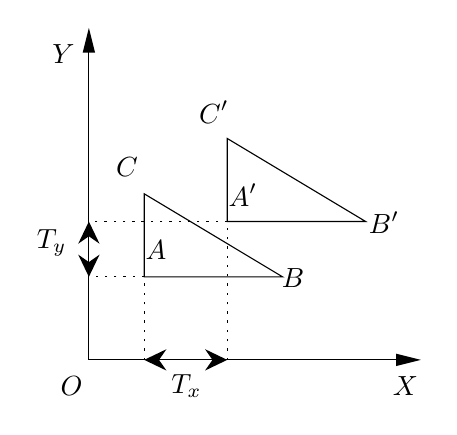
\begin{tikzpicture}[x=0.75pt,y=0.75pt,yscale=-1,xscale=1]
%uncomment if require: \path (0,310); %set diagram left start at 0, and has height of 310

%Straight Lines [id:da0744643818390529] 
\draw    (160,160) -- (160,133.33) -- (160,106.67) -- (160,80) -- (160,53.33) -- (160,26.67) -- (160,2) ;
\draw [shift={(160,0)}, rotate = 90] [fill={rgb, 255:red, 0; green, 0; blue, 0 }  ][line width=0.08]  [draw opacity=0] (12,-3) -- (0,0) -- (12,3) -- cycle    ;
%Straight Lines [id:da2501910192394292] 
\draw    (160,160) -- (186.67,160) -- (213.33,160) -- (240,160) -- (266.67,160) -- (293.33,160) -- (318,160) ;
\draw [shift={(320,160)}, rotate = 180] [fill={rgb, 255:red, 0; green, 0; blue, 0 }  ][line width=0.08]  [draw opacity=0] (12,-3) -- (0,0) -- (12,3) -- cycle    ;
%Shape: Right Triangle [id:dp3230440420217635] 
\draw   (186.67,80) -- (253.33,120) -- (186.67,120) -- cycle ;
%Straight Lines [id:da4274444095380905] 
\draw  [dash pattern={on 0.84pt off 2.51pt}]  (186.67,120) -- (160,120) ;
%Shape: Right Triangle [id:dp3554215710083837] 
\draw   (226.67,53.33) -- (293.33,93.33) -- (226.67,93.33) -- cycle ;
%Straight Lines [id:da18015886667211856] 
\draw  [dash pattern={on 0.84pt off 2.51pt}]  (226.67,93.33) -- (160,93.33) ;
%Straight Lines [id:da20825596809464475] 
\draw  [dash pattern={on 0.84pt off 2.51pt}]  (186.67,160) -- (186.67,137.12) -- (186.67,120) ;
%Straight Lines [id:da30415316219723487] 
\draw  [dash pattern={on 0.84pt off 2.51pt}]  (226.67,160) -- (226.67,93.33) ;
%Straight Lines [id:da18553363748469254] 
\draw    (189.67,160) -- (223.67,160) ;
\draw [shift={(226.67,160)}, rotate = 180] [fill={rgb, 255:red, 0; green, 0; blue, 0 }  ][line width=0.08]  [draw opacity=0] (10.72,-5.15) -- (0,0) -- (10.72,5.15) -- (7.12,0) -- cycle    ;
\draw [shift={(186.67,160)}, rotate = 0] [fill={rgb, 255:red, 0; green, 0; blue, 0 }  ][line width=0.08]  [draw opacity=0] (10.72,-5.15) -- (0,0) -- (10.72,5.15) -- (7.12,0) -- cycle    ;
%Straight Lines [id:da7758481926901326] 
\draw    (160,96.33) -- (160,117) ;
\draw [shift={(160,120)}, rotate = 270] [fill={rgb, 255:red, 0; green, 0; blue, 0 }  ][line width=0.08]  [draw opacity=0] (10.72,-5.15) -- (0,0) -- (10.72,5.15) -- (7.12,0) -- cycle    ;
\draw [shift={(160,93.33)}, rotate = 90] [fill={rgb, 255:red, 0; green, 0; blue, 0 }  ][line width=0.08]  [draw opacity=0] (10.72,-5.15) -- (0,0) -- (10.72,5.15) -- (7.12,0) -- cycle    ;

% Text Node
\draw (312.88,172.78) node   [align=left] {\begin{minipage}[lt]{9.68pt}\setlength\topsep{0pt}
$\displaystyle X$
\end{minipage}};
% Text Node
\draw (150.8,12.78) node   [align=left] {\begin{minipage}[lt]{12.51pt}\setlength\topsep{0pt}
$\displaystyle Y$
\end{minipage}};
% Text Node
\draw (152.88,172.78) node   [align=left] {\begin{minipage}[lt]{9.68pt}\setlength\topsep{0pt}
$\displaystyle O$
\end{minipage}};
% Text Node
\draw (193.79,107.22) node   [align=left] {\begin{minipage}[lt]{9.68pt}\setlength\topsep{0pt}
$\displaystyle A$
\end{minipage}};
% Text Node
\draw (233.79,80.55) node   [align=left] {\begin{minipage}[lt]{9.68pt}\setlength\topsep{0pt}
$\displaystyle A'$
\end{minipage}};
% Text Node
\draw (258.71,120.4) node   [align=left] {\begin{minipage}[lt]{8.67pt}\setlength\topsep{0pt}
$\displaystyle B$
\end{minipage}};
% Text Node
\draw (300.71,94) node   [align=left] {\begin{minipage}[lt]{8.67pt}\setlength\topsep{0pt}
$\displaystyle B'$
\end{minipage}};
% Text Node
\draw (179.55,67.22) node   [align=left] {\begin{minipage}[lt]{9.68pt}\setlength\topsep{0pt}
$\displaystyle C$
\end{minipage}};
% Text Node
\draw (219.55,40.55) node   [align=left] {\begin{minipage}[lt]{9.68pt}\setlength\topsep{0pt}
$\displaystyle C'$
\end{minipage}};
% Text Node
\draw (206.21,172.78) node   [align=left] {\begin{minipage}[lt]{9.68pt}\setlength\topsep{0pt}
$\displaystyle T_{x}$
\end{minipage}};
% Text Node
\draw (141.41,103.58) node   [align=left] {\begin{minipage}[lt]{9.68pt}\setlength\topsep{0pt}
$\displaystyle T_{y}$
\end{minipage}};


\end{tikzpicture}

    }
    \subfigure[scale=.9][比例系数 $S_x=S_y=1$]{
        

\tikzset{every picture/.style={line width=0.75pt}} %set default line width to 0.75pt        

\begin{tikzpicture}[x=0.75pt,y=0.75pt,yscale=-1,xscale=1]
%uncomment if require: \path (0,310); %set diagram left start at 0, and has height of 310

%Straight Lines [id:da15250042942435282] 
\draw    (160,160) -- (160,133.33) -- (160,106.67) -- (160,80) -- (160,53.33) -- (160,26.67) -- (160,2) ;
\draw [shift={(160,0)}, rotate = 90] [fill={rgb, 255:red, 0; green, 0; blue, 0 }  ][line width=0.08]  [draw opacity=0] (12,-3) -- (0,0) -- (12,3) -- cycle    ;
%Straight Lines [id:da8576603280236559] 
\draw    (160,160) -- (186.67,160) -- (213.33,160) -- (240,160) -- (266.67,160) -- (293.33,160) -- (318,160) ;
\draw [shift={(320,160)}, rotate = 180] [fill={rgb, 255:red, 0; green, 0; blue, 0 }  ][line width=0.08]  [draw opacity=0] (12,-3) -- (0,0) -- (12,3) -- cycle    ;
%Shape: Right Triangle [id:dp7502598031763401] 
\draw   (186.67,80) -- (253.33,120) -- (186.67,120) -- cycle ;

% Text Node
\draw (312.88,172.78) node   [align=left] {\begin{minipage}[lt]{9.68pt}\setlength\topsep{0pt}
$\displaystyle X$
\end{minipage}};
% Text Node
\draw (150.8,12.78) node   [align=left] {\begin{minipage}[lt]{12.51pt}\setlength\topsep{0pt}
$\displaystyle Y$
\end{minipage}};
% Text Node
\draw (152.88,172.78) node   [align=left] {\begin{minipage}[lt]{9.68pt}\setlength\topsep{0pt}
$\displaystyle O$
\end{minipage}};
% Text Node
\draw (178.21,107.22) node   [align=left] {\begin{minipage}[lt]{11.5pt}\setlength\topsep{0pt}
$\displaystyle A$
\end{minipage}};
% Text Node
\draw (193.79,107.22) node   [align=left] {\begin{minipage}[lt]{9.68pt}\setlength\topsep{0pt}
$\displaystyle A'$
\end{minipage}};
% Text Node
\draw (247.59,132.78) node   [align=left] {\begin{minipage}[lt]{8.67pt}\setlength\topsep{0pt}
$\displaystyle B$
\end{minipage}};
% Text Node
\draw (259.08,132.78) node   [align=left] {\begin{minipage}[lt]{8.67pt}\setlength\topsep{0pt}
$\displaystyle B'$
\end{minipage}};
% Text Node
\draw (179.55,67.22) node   [align=left] {\begin{minipage}[lt]{9.68pt}\setlength\topsep{0pt}
$\displaystyle C$
\end{minipage}};
% Text Node
\draw (193.79,67.22) node   [align=left] {\begin{minipage}[lt]{9.68pt}\setlength\topsep{0pt}
$\displaystyle C'$
\end{minipage}};


\end{tikzpicture}
    }
    \subfigure[scale=.9][比例系数 $S_x=S_y>1$]{
        

\tikzset{every picture/.style={line width=0.75pt}} %set default line width to 0.75pt        

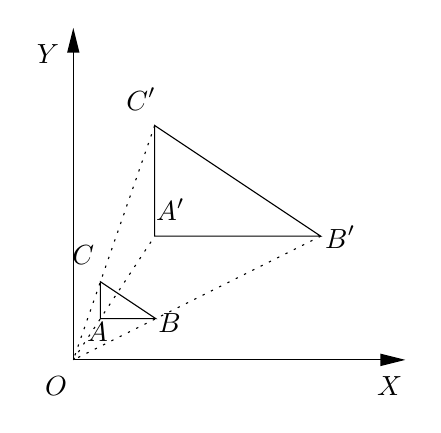
\begin{tikzpicture}[x=0.75pt,y=0.75pt,yscale=-1,xscale=1]
%uncomment if require: \path (0,310); %set diagram left start at 0, and has height of 310

%Straight Lines [id:da1534328502257163] 
\draw    (160,160) -- (160,133.33) -- (160,106.67) -- (160,80) -- (160,53.33) -- (160,26.67) -- (160,2) ;
\draw [shift={(160,0)}, rotate = 90] [fill={rgb, 255:red, 0; green, 0; blue, 0 }  ][line width=0.08]  [draw opacity=0] (12,-3) -- (0,0) -- (12,3) -- cycle    ;
%Straight Lines [id:da05091810398310703] 
\draw    (160,160) -- (186.67,160) -- (213.33,160) -- (240,160) -- (266.67,160) -- (293.33,160) -- (318,160) ;
\draw [shift={(320,160)}, rotate = 180] [fill={rgb, 255:red, 0; green, 0; blue, 0 }  ][line width=0.08]  [draw opacity=0] (12,-3) -- (0,0) -- (12,3) -- cycle    ;
%Shape: Right Triangle [id:dp7699621838177173] 
\draw   (199.2,47.07) -- (279.2,100.4) -- (199.2,100.4) -- cycle ;
%Shape: Right Triangle [id:dp6819256437414682] 
\draw   (173.07,122.36) -- (199.73,140.13) -- (173.07,140.13) -- cycle ;
%Straight Lines [id:da5214539639167379] 
\draw  [dash pattern={on 0.84pt off 2.51pt}]  (199.2,47.07) -- (192.67,65.89) -- (186.13,84.71) -- (179.6,103.53) -- (173.07,122.36) -- (166.53,141.18) -- (160,160) ;
%Straight Lines [id:da8425910163250174] 
\draw  [dash pattern={on 0.84pt off 2.51pt}]  (279.2,100.4) -- (259.33,110.33) -- (239.47,120.27) -- (219.6,130.2) -- (199.73,140.13) -- (179.87,150.07) -- (160,160) ;
%Straight Lines [id:da47875893336700104] 
\draw  [dash pattern={on 0.84pt off 2.51pt}]  (160,160) -- (199.2,100.4) ;

% Text Node
\draw (312.88,172.78) node   [align=left] {\begin{minipage}[lt]{9.68pt}\setlength\topsep{0pt}
$\displaystyle X$
\end{minipage}};
% Text Node
\draw (150.8,12.78) node   [align=left] {\begin{minipage}[lt]{12.51pt}\setlength\topsep{0pt}
$\displaystyle Y$
\end{minipage}};
% Text Node
\draw (152.88,172.78) node   [align=left] {\begin{minipage}[lt]{9.68pt}\setlength\topsep{0pt}
$\displaystyle O$
\end{minipage}};
% Text Node
\draw (173.12,146.42) node   [align=left] {\begin{minipage}[lt]{9.68pt}\setlength\topsep{0pt}
$\displaystyle A$
\end{minipage}};
% Text Node
\draw (206.32,87.62) node   [align=left] {\begin{minipage}[lt]{9.68pt}\setlength\topsep{0pt}
$\displaystyle A'$
\end{minipage}};
% Text Node
\draw (206.71,142.4) node   [align=left] {\begin{minipage}[lt]{8.67pt}\setlength\topsep{0pt}
$\displaystyle B$
\end{minipage}};
% Text Node
\draw (287.11,100.8) node   [align=left] {\begin{minipage}[lt]{8.67pt}\setlength\topsep{0pt}
$\displaystyle B'$
\end{minipage}};
% Text Node
\draw (165.95,109.58) node   [align=left] {\begin{minipage}[lt]{9.68pt}\setlength\topsep{0pt}
$\displaystyle C$
\end{minipage}};
% Text Node
\draw (192.08,34.29) node   [align=left] {\begin{minipage}[lt]{9.68pt}\setlength\topsep{0pt}
$\displaystyle C'$
\end{minipage}};


\end{tikzpicture}

    }
    \subfigure[scale=.9][比例系数 $0<S_x=S_y<1$]{
        

\tikzset{every picture/.style={line width=0.75pt}} %set default line width to 0.75pt        

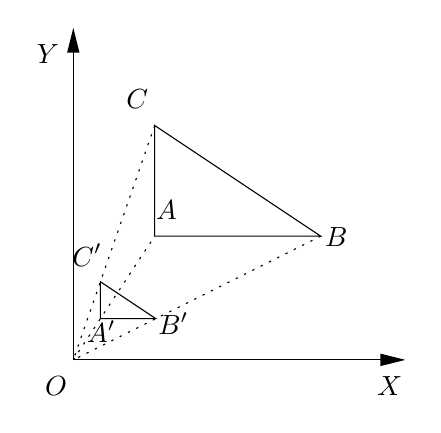
\begin{tikzpicture}[x=0.75pt,y=0.75pt,yscale=-1,xscale=1]
%uncomment if require: \path (0,310); %set diagram left start at 0, and has height of 310

%Straight Lines [id:da9243963150205441] 
\draw    (160,160) -- (160,133.33) -- (160,106.67) -- (160,80) -- (160,53.33) -- (160,26.67) -- (160,2) ;
\draw [shift={(160,0)}, rotate = 90] [fill={rgb, 255:red, 0; green, 0; blue, 0 }  ][line width=0.08]  [draw opacity=0] (12,-3) -- (0,0) -- (12,3) -- cycle    ;
%Straight Lines [id:da8002028753633985] 
\draw    (160,160) -- (186.67,160) -- (213.33,160) -- (240,160) -- (266.67,160) -- (293.33,160) -- (318,160) ;
\draw [shift={(320,160)}, rotate = 180] [fill={rgb, 255:red, 0; green, 0; blue, 0 }  ][line width=0.08]  [draw opacity=0] (12,-3) -- (0,0) -- (12,3) -- cycle    ;
%Shape: Right Triangle [id:dp3074265042318134] 
\draw   (199.2,47.07) -- (279.2,100.4) -- (199.2,100.4) -- cycle ;
%Shape: Right Triangle [id:dp29770002438414234] 
\draw   (173.07,122.36) -- (199.73,140.13) -- (173.07,140.13) -- cycle ;
%Straight Lines [id:da024412753399659648] 
\draw  [dash pattern={on 0.84pt off 2.51pt}]  (199.2,47.07) -- (192.67,65.89) -- (186.13,84.71) -- (179.6,103.53) -- (173.07,122.36) -- (166.53,141.18) -- (160,160) ;
%Straight Lines [id:da7095636127854406] 
\draw  [dash pattern={on 0.84pt off 2.51pt}]  (279.2,100.4) -- (259.33,110.33) -- (239.47,120.27) -- (219.6,130.2) -- (199.73,140.13) -- (179.87,150.07) -- (160,160) ;
%Straight Lines [id:da5652492210181941] 
\draw  [dash pattern={on 0.84pt off 2.51pt}]  (160,160) -- (199.2,100.4) ;

% Text Node
\draw (312.88,172.78) node   [align=left] {\begin{minipage}[lt]{9.68pt}\setlength\topsep{0pt}
$\displaystyle X$
\end{minipage}};
% Text Node
\draw (150.8,12.78) node   [align=left] {\begin{minipage}[lt]{12.51pt}\setlength\topsep{0pt}
$\displaystyle Y$
\end{minipage}};
% Text Node
\draw (152.88,172.78) node   [align=left] {\begin{minipage}[lt]{9.68pt}\setlength\topsep{0pt}
$\displaystyle O$
\end{minipage}};
% Text Node
\draw (173.12,146.42) node   [align=left] {\begin{minipage}[lt]{9.68pt}\setlength\topsep{0pt}
$\displaystyle A'$
\end{minipage}};
% Text Node
\draw (206.32,87.62) node   [align=left] {\begin{minipage}[lt]{9.68pt}\setlength\topsep{0pt}
$\displaystyle A$
\end{minipage}};
% Text Node
\draw (206.71,142.4) node   [align=left] {\begin{minipage}[lt]{8.67pt}\setlength\topsep{0pt}
$\displaystyle B'$
\end{minipage}};
% Text Node
\draw (287.11,100.8) node   [align=left] {\begin{minipage}[lt]{8.67pt}\setlength\topsep{0pt}
$\displaystyle B$
\end{minipage}};
% Text Node
\draw (165.95,109.58) node   [align=left] {\begin{minipage}[lt]{9.68pt}\setlength\topsep{0pt}
$\displaystyle C'$
\end{minipage}};
% Text Node
\draw (192.08,34.29) node   [align=left] {\begin{minipage}[lt]{9.68pt}\setlength\topsep{0pt}
$\displaystyle C$
\end{minipage}};


\end{tikzpicture}

    }
    \subfigure[scale=.9][$S_x=1,~S_y>1$]{
        

\tikzset{every picture/.style={line width=0.75pt}} %set default line width to 0.75pt        

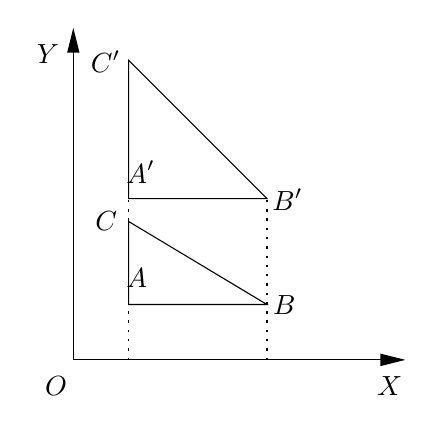
\begin{tikzpicture}[x=0.75pt,y=0.75pt,yscale=-1,xscale=1]
%uncomment if require: \path (0,310); %set diagram left start at 0, and has height of 310

%Straight Lines [id:da8557514491265967] 
\draw    (160,160) -- (160,133.33) -- (160,106.67) -- (160,80) -- (160,53.33) -- (160,26.67) -- (160,2) ;
\draw [shift={(160,0)}, rotate = 90] [fill={rgb, 255:red, 0; green, 0; blue, 0 }  ][line width=0.08]  [draw opacity=0] (12,-3) -- (0,0) -- (12,3) -- cycle    ;
%Straight Lines [id:da5539450143531788] 
\draw    (160,160) -- (186.67,160) -- (213.33,160) -- (240,160) -- (266.67,160) -- (293.33,160) -- (318,160) ;
\draw [shift={(320,160)}, rotate = 180] [fill={rgb, 255:red, 0; green, 0; blue, 0 }  ][line width=0.08]  [draw opacity=0] (12,-3) -- (0,0) -- (12,3) -- cycle    ;
%Straight Lines [id:da5193682179432797] 
\draw  [dash pattern={on 0.84pt off 2.51pt}]  (186.67,160) -- (186.67,82.33) ;
%Shape: Right Triangle [id:dp8688230494789257] 
\draw   (186.67,93.33) -- (253.33,133.33) -- (186.67,133.33) -- cycle ;
%Shape: Right Triangle [id:dp373344497154698] 
\draw   (186.67,15.67) -- (253.33,82.33) -- (186.67,82.33) -- cycle ;
%Straight Lines [id:da7747623883965025] 
\draw  [dash pattern={on 0.84pt off 2.51pt}]  (253.33,160) -- (253.33,82.33) ;

% Text Node
\draw (312.88,172.78) node   [align=left] {\begin{minipage}[lt]{9.68pt}\setlength\topsep{0pt}
$\displaystyle X$
\end{minipage}};
% Text Node
\draw (150.8,12.78) node   [align=left] {\begin{minipage}[lt]{12.51pt}\setlength\topsep{0pt}
$\displaystyle Y$
\end{minipage}};
% Text Node
\draw (152.88,172.78) node   [align=left] {\begin{minipage}[lt]{9.68pt}\setlength\topsep{0pt}
$\displaystyle O$
\end{minipage}};
% Text Node
\draw (191.4,69.55) node   [align=left] {\begin{minipage}[lt]{8.67pt}\setlength\topsep{0pt}
$\displaystyle A'$
\end{minipage}};
% Text Node
\draw (191.4,120.55) node   [align=left] {\begin{minipage}[lt]{8.67pt}\setlength\topsep{0pt}
$\displaystyle A$
\end{minipage}};
% Text Node
\draw (261.71,82.73) node   [align=left] {\begin{minipage}[lt]{8.67pt}\setlength\topsep{0pt}
$\displaystyle B'$
\end{minipage}};
% Text Node
\draw (262.11,133.47) node   [align=left] {\begin{minipage}[lt]{8.67pt}\setlength\topsep{0pt}
$\displaystyle B$
\end{minipage}};
% Text Node
\draw (174.95,16.24) node   [align=left] {\begin{minipage}[lt]{9.68pt}\setlength\topsep{0pt}
$\displaystyle C'$
\end{minipage}};
% Text Node
\draw (177.08,92.95) node   [align=left] {\begin{minipage}[lt]{9.68pt}\setlength\topsep{0pt}
$\displaystyle C$
\end{minipage}};


\end{tikzpicture}

    }
    \subfigure[scale=.9][$Y$ 轴对称]{
        

\tikzset{every picture/.style={line width=0.75pt}} %set default line width to 0.75pt        

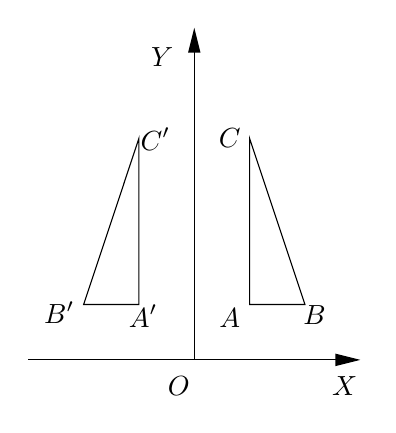
\begin{tikzpicture}[x=0.75pt,y=0.75pt,yscale=-1,xscale=1]
%uncomment if require: \path (0,310); %set diagram left start at 0, and has height of 310

%Straight Lines [id:da9473706495657213] 
\draw    (240,160) -- (240,133.33) -- (240,106.67) -- (240,80) -- (240,53.33) -- (240,26.67) -- (240,2) ;
\draw [shift={(240,0)}, rotate = 90] [fill={rgb, 255:red, 0; green, 0; blue, 0 }  ][line width=0.08]  [draw opacity=0] (12,-3) -- (0,0) -- (12,3) -- cycle    ;
%Straight Lines [id:da3401945044692589] 
\draw    (160,160) -- (186.67,160) -- (213.33,160) -- (240,160) -- (266.67,160) -- (293.33,160) -- (318,160) ;
\draw [shift={(320,160)}, rotate = 180] [fill={rgb, 255:red, 0; green, 0; blue, 0 }  ][line width=0.08]  [draw opacity=0] (12,-3) -- (0,0) -- (12,3) -- cycle    ;
%Shape: Right Triangle [id:dp2883900535142023] 
\draw   (266.67,53.33) -- (293.33,133.33) -- (266.67,133.33) -- cycle ;
%Shape: Right Triangle [id:dp0361672463144318] 
\draw   (213.33,53.33) -- (186.67,133.33) -- (213.33,133.33) -- cycle ;

% Text Node
\draw (312.88,172.78) node   [align=left] {\begin{minipage}[lt]{9.68pt}\setlength\topsep{0pt}
$\displaystyle X$
\end{minipage}};
% Text Node
\draw (227.6,13.98) node   [align=left] {\begin{minipage}[lt]{12.51pt}\setlength\topsep{0pt}
$\displaystyle Y$
\end{minipage}};
% Text Node
\draw (233.79,172.78) node   [align=left] {\begin{minipage}[lt]{9.68pt}\setlength\topsep{0pt}
$\displaystyle O$
\end{minipage}};
% Text Node
\draw (259.81,139.62) node   [align=left] {\begin{minipage}[lt]{11.5pt}\setlength\topsep{0pt}
$\displaystyle A$
\end{minipage}};
% Text Node
\draw (214.99,138.82) node   [align=left] {\begin{minipage}[lt]{9.68pt}\setlength\topsep{0pt}
$\displaystyle A'$
\end{minipage}};
% Text Node
\draw (298.39,138.38) node   [align=left] {\begin{minipage}[lt]{8.67pt}\setlength\topsep{0pt}
$\displaystyle B$
\end{minipage}};
% Text Node
\draw (173.48,137.18) node   [align=left] {\begin{minipage}[lt]{8.67pt}\setlength\topsep{0pt}
$\displaystyle B'$
\end{minipage}};
% Text Node
\draw (258.35,53.22) node   [align=left] {\begin{minipage}[lt]{9.68pt}\setlength\topsep{0pt}
$\displaystyle C$
\end{minipage}};
% Text Node
\draw (220.59,53.62) node   [align=left] {\begin{minipage}[lt]{9.68pt}\setlength\topsep{0pt}
$\displaystyle C'$
\end{minipage}};


\end{tikzpicture}

    }
    \subfigure[scale=.9][$X$ 轴对称]{
        

\tikzset{every picture/.style={line width=0.75pt}} %set default line width to 0.75pt        

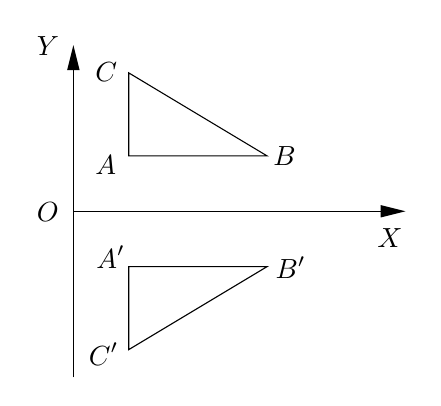
\begin{tikzpicture}[x=0.75pt,y=0.75pt,yscale=-1,xscale=1]
%uncomment if require: \path (0,310); %set diagram left start at 0, and has height of 310

%Straight Lines [id:da24368355678437692] 
\draw    (160,240) -- (160,213.33) -- (160,186.67) -- (160,160) -- (160,133.33) -- (160,106.67) -- (160,82) ;
\draw [shift={(160,80)}, rotate = 90] [fill={rgb, 255:red, 0; green, 0; blue, 0 }  ][line width=0.08]  [draw opacity=0] (12,-3) -- (0,0) -- (12,3) -- cycle    ;
%Straight Lines [id:da91989606623083] 
\draw    (160,160) -- (186.67,160) -- (213.33,160) -- (240,160) -- (266.67,160) -- (293.33,160) -- (318,160) ;
\draw [shift={(320,160)}, rotate = 180] [fill={rgb, 255:red, 0; green, 0; blue, 0 }  ][line width=0.08]  [draw opacity=0] (12,-3) -- (0,0) -- (12,3) -- cycle    ;
%Shape: Right Triangle [id:dp6047665119381709] 
\draw   (186.67,93.33) -- (253.33,133.33) -- (186.67,133.33) -- cycle ;
%Shape: Right Triangle [id:dp2085112249426042] 
\draw   (186.67,226.67) -- (253.33,186.67) -- (186.67,186.67) -- cycle ;

% Text Node
\draw (312.88,172.78) node   [align=left] {\begin{minipage}[lt]{9.68pt}\setlength\topsep{0pt}
$\displaystyle X$
\end{minipage}};
% Text Node
\draw (150.8,80.55) node   [align=left] {\begin{minipage}[lt]{12.51pt}\setlength\topsep{0pt}
$\displaystyle Y$
\end{minipage}};
% Text Node
\draw (148.88,160.28) node   [align=left] {\begin{minipage}[lt]{9.68pt}\setlength\topsep{0pt}
$\displaystyle O$
\end{minipage}};
% Text Node
\draw (176.9,182.05) node   [align=left] {\begin{minipage}[lt]{8.67pt}\setlength\topsep{0pt}
$\displaystyle A'$
\end{minipage}};
% Text Node
\draw (176.4,137.55) node   [align=left] {\begin{minipage}[lt]{8.67pt}\setlength\topsep{0pt}
$\displaystyle A$
\end{minipage}};
% Text Node
\draw (263.21,187.23) node   [align=left] {\begin{minipage}[lt]{8.67pt}\setlength\topsep{0pt}
$\displaystyle B'$
\end{minipage}};
% Text Node
\draw (262.11,133.47) node   [align=left] {\begin{minipage}[lt]{8.67pt}\setlength\topsep{0pt}
$\displaystyle B$
\end{minipage}};
% Text Node
\draw (173.95,228.74) node   [align=left] {\begin{minipage}[lt]{9.68pt}\setlength\topsep{0pt}
$\displaystyle C'$
\end{minipage}};
% Text Node
\draw (177.08,92.95) node   [align=left] {\begin{minipage}[lt]{9.68pt}\setlength\topsep{0pt}
$\displaystyle C$
\end{minipage}};


\end{tikzpicture}

    }
    \subfigure[scale=.9][中心对称]{
        

\tikzset{every picture/.style={line width=0.75pt}} %set default line width to 0.75pt        

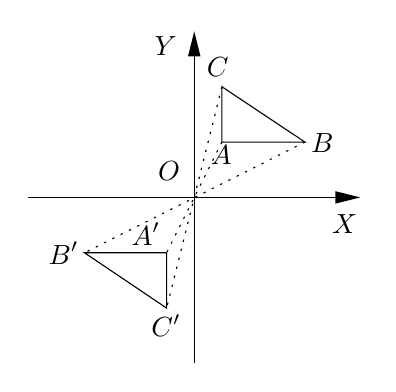
\begin{tikzpicture}[x=0.75pt,y=0.75pt,yscale=-1,xscale=1]
%uncomment if require: \path (0,310); %set diagram left start at 0, and has height of 310

%Straight Lines [id:da20466553477334037] 
\draw    (240,240) -- (240,213.33) -- (240,186.67) -- (240,160) -- (240,133.33) -- (240,106.67) -- (240,82) ;
\draw [shift={(240,80)}, rotate = 90] [fill={rgb, 255:red, 0; green, 0; blue, 0 }  ][line width=0.08]  [draw opacity=0] (12,-3) -- (0,0) -- (12,3) -- cycle    ;
%Straight Lines [id:da07906371106904819] 
\draw    (160,160) -- (186.67,160) -- (213.33,160) -- (240,160) -- (266.67,160) -- (293.33,160) -- (318,160) ;
\draw [shift={(320,160)}, rotate = 180] [fill={rgb, 255:red, 0; green, 0; blue, 0 }  ][line width=0.08]  [draw opacity=0] (12,-3) -- (0,0) -- (12,3) -- cycle    ;
%Shape: Right Triangle [id:dp711098921084359] 
\draw   (253.33,106.67) -- (293.33,133.33) -- (253.33,133.33) -- cycle ;
%Shape: Right Triangle [id:dp32855978989430157] 
\draw   (226.67,213.33) -- (187.13,186.67) -- (226.67,186.67) -- cycle ;
%Straight Lines [id:da813083554485903] 
\draw  [dash pattern={on 0.84pt off 2.51pt}]  (253.33,133.33) -- (226.67,186.67) ;
%Straight Lines [id:da3857126514317757] 
\draw  [dash pattern={on 0.84pt off 2.51pt}]  (293.33,133.33) -- (187.13,186.67) ;
%Straight Lines [id:da811525310685079] 
\draw  [dash pattern={on 0.84pt off 2.51pt}]  (253.33,106.67) -- (226.67,213.33) ;

% Text Node
\draw (312.88,172.78) node   [align=left] {\begin{minipage}[lt]{9.68pt}\setlength\topsep{0pt}
$\displaystyle X$
\end{minipage}};
% Text Node
\draw (229.2,87.22) node   [align=left] {\begin{minipage}[lt]{12.51pt}\setlength\topsep{0pt}
$\displaystyle Y$
\end{minipage}};
% Text Node
\draw (230.85,147.22) node   [align=left] {\begin{minipage}[lt]{12.44pt}\setlength\topsep{0pt}
$\displaystyle O$
\end{minipage}};
% Text Node
\draw (255.71,139.72) node   [align=left] {\begin{minipage}[lt]{11.5pt}\setlength\topsep{0pt}
$\displaystyle A$
\end{minipage}};
% Text Node
\draw (216.29,177.72) node   [align=left] {\begin{minipage}[lt]{9.68pt}\setlength\topsep{0pt}
$\displaystyle A'$
\end{minipage}};
% Text Node
\draw (302.09,133.78) node   [align=left] {\begin{minipage}[lt]{8.67pt}\setlength\topsep{0pt}
$\displaystyle B$
\end{minipage}};
% Text Node
\draw (175.58,186.78) node   [align=left] {\begin{minipage}[lt]{8.67pt}\setlength\topsep{0pt}
$\displaystyle B'$
\end{minipage}};
% Text Node
\draw (252.55,97.22) node   [align=left] {\begin{minipage}[lt]{9.68pt}\setlength\topsep{0pt}
$\displaystyle C$
\end{minipage}};
% Text Node
\draw (225.79,221.72) node   [align=left] {\begin{minipage}[lt]{9.68pt}\setlength\topsep{0pt}
$\displaystyle C'$
\end{minipage}};


\end{tikzpicture}

    }
    \subfigure[scale=.9][$Y=X$ 对称]{
        

\tikzset{every picture/.style={line width=0.75pt}} %set default line width to 0.75pt        

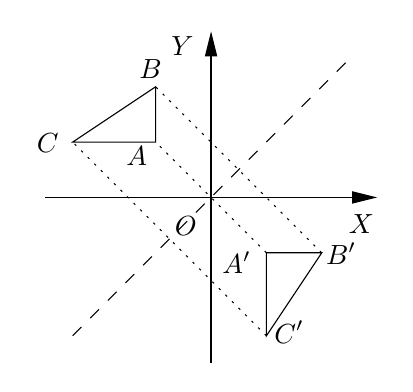
\begin{tikzpicture}[x=0.75pt,y=0.75pt,yscale=-1,xscale=1]
%uncomment if require: \path (0,310); %set diagram left start at 0, and has height of 310

%Straight Lines [id:da8292659722722793] 
\draw    (240,240) -- (240,213.33) -- (240,186.67) -- (240,160) -- (240,133.33) -- (240,106.67) -- (240,82) ;
\draw [shift={(240,80)}, rotate = 90] [fill={rgb, 255:red, 0; green, 0; blue, 0 }  ][line width=0.08]  [draw opacity=0] (12,-3) -- (0,0) -- (12,3) -- cycle    ;
%Straight Lines [id:da7352149228464684] 
\draw    (160,160) -- (186.67,160) -- (213.33,160) -- (240,160) -- (266.67,160) -- (293.33,160) -- (318,160) ;
\draw [shift={(320,160)}, rotate = 180] [fill={rgb, 255:red, 0; green, 0; blue, 0 }  ][line width=0.08]  [draw opacity=0] (12,-3) -- (0,0) -- (12,3) -- cycle    ;
%Straight Lines [id:da2661475178458712] 
\draw  [dash pattern={on 0.84pt off 2.51pt}]  (266.67,186.67) -- (213.33,133.33) ;
%Shape: Right Triangle [id:dp6596390866394817] 
\draw   (213.33,106.67) -- (173.33,133.33) -- (213.33,133.33) -- cycle ;
%Straight Lines [id:da7951069745564614] 
\draw  [dash pattern={on 4.5pt off 4.5pt}]  (173.33,226.67) -- (306.67,93.33) ;
%Shape: Right Triangle [id:dp32508442712015806] 
\draw   (266.67,226.67) -- (293.33,186.67) -- (266.67,186.67) -- cycle ;
%Straight Lines [id:da9943714913243453] 
\draw  [dash pattern={on 0.84pt off 2.51pt}]  (293.33,186.67) -- (213.33,106.67) ;
%Straight Lines [id:da42142200377858186] 
\draw  [dash pattern={on 0.84pt off 2.51pt}]  (266.67,226.67) -- (173.33,133.33) ;

% Text Node
\draw (312.88,172.78) node   [align=left] {\begin{minipage}[lt]{9.68pt}\setlength\topsep{0pt}
$\displaystyle X$
\end{minipage}};
% Text Node
\draw (229.2,87.22) node   [align=left] {\begin{minipage}[lt]{12.51pt}\setlength\topsep{0pt}
$\displaystyle Y$
\end{minipage}};
% Text Node
\draw (230.85,173.89) node   [align=left] {\begin{minipage}[lt]{12.44pt}\setlength\topsep{0pt}
$\displaystyle O$
\end{minipage}};
% Text Node
\draw (206.91,140.12) node   [align=left] {\begin{minipage}[lt]{11.5pt}\setlength\topsep{0pt}
$\displaystyle A$
\end{minipage}};
% Text Node
\draw (251.89,191.32) node   [align=left] {\begin{minipage}[lt]{9.68pt}\setlength\topsep{0pt}
$\displaystyle A'$
\end{minipage}};
% Text Node
\draw (211.29,98.18) node   [align=left] {\begin{minipage}[lt]{8.67pt}\setlength\topsep{0pt}
$\displaystyle B$
\end{minipage}};
% Text Node
\draw (301.18,187.18) node   [align=left] {\begin{minipage}[lt]{8.67pt}\setlength\topsep{0pt}
$\displaystyle B'$
\end{minipage}};
% Text Node
\draw (162.55,134.02) node   [align=left] {\begin{minipage}[lt]{9.68pt}\setlength\topsep{0pt}
$\displaystyle C$
\end{minipage}};
% Text Node
\draw (276.99,224.92) node   [align=left] {\begin{minipage}[lt]{9.68pt}\setlength\topsep{0pt}
$\displaystyle C'$
\end{minipage}};


\end{tikzpicture}

    }
    \subfigure[scale=.9][$Y=-X$ 对称]{
        

\tikzset{every picture/.style={line width=0.75pt}} %set default line width to 0.75pt        

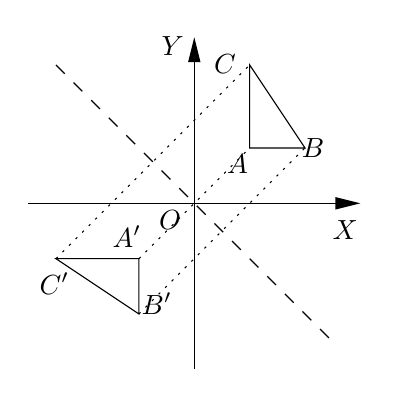
\begin{tikzpicture}[x=0.75pt,y=0.75pt,yscale=-1,xscale=1]
%uncomment if require: \path (0,310); %set diagram left start at 0, and has height of 310

%Straight Lines [id:da2266867895070097] 
\draw    (155.13,159.59) -- (181.8,159.59) -- (208.47,159.59) -- (235.13,159.59) -- (261.8,159.59) -- (288.47,159.59) -- (313.13,159.59) ;
\draw [shift={(315.13,159.59)}, rotate = 180] [fill={rgb, 255:red, 0; green, 0; blue, 0 }  ][line width=0.08]  [draw opacity=0] (12,-3) -- (0,0) -- (12,3) -- cycle    ;
%Straight Lines [id:da4885018729597703] 
\draw    (235.13,81.59) -- (235.13,106.25) -- (235.13,132.92) -- (235.13,159.59) -- (235.13,186.25) -- (235.13,212.92) -- (235.13,239.59) ;
\draw [shift={(235.13,79.59)}, rotate = 90] [fill={rgb, 255:red, 0; green, 0; blue, 0 }  ][line width=0.08]  [draw opacity=0] (12,-3) -- (0,0) -- (12,3) -- cycle    ;
%Straight Lines [id:da37798418466605876] 
\draw  [dash pattern={on 0.84pt off 2.51pt}]  (208.47,186.25) -- (261.8,132.92) ;
%Shape: Right Triangle [id:dp9937709437984665] 
\draw   (288.47,132.92) -- (261.8,92.92) -- (261.8,132.92) -- cycle ;
%Straight Lines [id:da8376057486917463] 
\draw  [dash pattern={on 4.5pt off 4.5pt}]  (168.47,92.92) -- (301.8,226.25) ;
%Shape: Right Triangle [id:dp15886819391939877] 
\draw   (168.47,186.25) -- (208.47,212.92) -- (208.47,186.25) -- cycle ;
%Straight Lines [id:da8724202073941834] 
\draw  [dash pattern={on 0.84pt off 2.51pt}]  (208.47,212.92) -- (288.47,132.92) ;
%Straight Lines [id:da8687627509248148] 
\draw  [dash pattern={on 0.84pt off 2.51pt}]  (168.47,186.25) -- (261.8,92.92) ;

% Text Node
\draw (307.55,172.37) node   [align=left] {\begin{minipage}[lt]{8.67pt}\setlength\topsep{0pt}
$\displaystyle X$
\end{minipage}};
% Text Node
\draw (225.15,83.97) node   [align=left] {\begin{minipage}[lt]{8.67pt}\setlength\topsep{0pt}
$\displaystyle Y$
\end{minipage}};
% Text Node
\draw (223.95,167.57) node   [align=left] {\begin{minipage}[lt]{8.67pt}\setlength\topsep{0pt}
$\displaystyle O$
\end{minipage}};
% Text Node
\draw (256.75,140.77) node   [align=left] {\begin{minipage}[lt]{8.67pt}\setlength\topsep{0pt}
$\displaystyle A$
\end{minipage}};
% Text Node
\draw (201.55,175.57) node   [align=left] {\begin{minipage}[lt]{8.67pt}\setlength\topsep{0pt}
$\displaystyle A'$
\end{minipage}};
% Text Node
\draw (292.75,133.17) node   [align=left] {\begin{minipage}[lt]{8.67pt}\setlength\topsep{0pt}
$\displaystyle B$
\end{minipage}};
% Text Node
\draw (250.45,92.54) node   [align=left] {\begin{minipage}[lt]{8.67pt}\setlength\topsep{0pt}
$\displaystyle C$
\end{minipage}};
% Text Node
\draw (215.55,207.97) node   [align=left] {\begin{minipage}[lt]{8.67pt}\setlength\topsep{0pt}
$\displaystyle B'$
\end{minipage}};
% Text Node
\draw (166.35,198.37) node   [align=left] {\begin{minipage}[lt]{8.67pt}\setlength\topsep{0pt}
$\displaystyle C'$
\end{minipage}};


\end{tikzpicture}

    }
    \subfigure[scale=.9][相对原点旋转 $\theta$ 角]{
        

\tikzset{every picture/.style={line width=0.75pt}} %set default line width to 0.75pt        

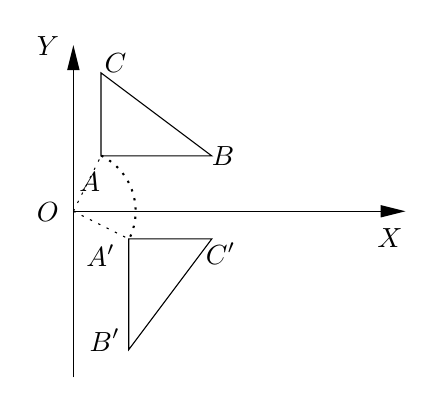
\begin{tikzpicture}[x=0.75pt,y=0.75pt,yscale=-1,xscale=1]
%uncomment if require: \path (0,310); %set diagram left start at 0, and has height of 310

%Straight Lines [id:da713951749740587] 
\draw    (160,240) -- (160,213.33) -- (160,186.67) -- (160,160) -- (160,133.33) -- (160,106.67) -- (160,82) ;
\draw [shift={(160,80)}, rotate = 90] [fill={rgb, 255:red, 0; green, 0; blue, 0 }  ][line width=0.08]  [draw opacity=0] (12,-3) -- (0,0) -- (12,3) -- cycle    ;
%Straight Lines [id:da27505852441502276] 
\draw    (160,160) -- (186.67,160) -- (213.33,160) -- (240,160) -- (266.67,160) -- (293.33,160) -- (318,160) ;
\draw [shift={(320,160)}, rotate = 180] [fill={rgb, 255:red, 0; green, 0; blue, 0 }  ][line width=0.08]  [draw opacity=0] (12,-3) -- (0,0) -- (12,3) -- cycle    ;
%Shape: Right Triangle [id:dp9653910433627337] 
\draw   (173.33,93.33) -- (226.67,133.33) -- (173.33,133.33) -- cycle ;
%Shape: Right Triangle [id:dp19153562200662932] 
\draw   (226.67,173.33) -- (186.67,226.67) -- (186.67,173.33) -- cycle ;
%Straight Lines [id:da6181416799790123] 
\draw  [dash pattern={on 0.84pt off 2.51pt}]  (160,160) -- (173.33,133.33) ;
%Straight Lines [id:da34341147568550356] 
\draw  [dash pattern={on 0.84pt off 2.51pt}]  (160,160) -- (186.67,173.33) ;
%Shape: Arc [id:dp3703274603787783] 
\draw  [draw opacity=0][dash pattern={on 0.84pt off 2.51pt}][line width=0.75]  (173.45,133.18) .. controls (183.26,138.11) and (190,148.27) .. (190,160) .. controls (190,164.85) and (188.85,169.43) .. (186.81,173.48) -- (160,160) -- cycle ; \draw  [dash pattern={on 0.84pt off 2.51pt}][line width=0.75]  (173.45,133.18) .. controls (183.26,138.11) and (190,148.27) .. (190,160) .. controls (190,164.85) and (188.85,169.43) .. (186.81,173.48) ;  

% Text Node
\draw (312.88,172.78) node   [align=left] {\begin{minipage}[lt]{9.68pt}\setlength\topsep{0pt}
$\displaystyle X$
\end{minipage}};
% Text Node
\draw (150.8,80.55) node   [align=left] {\begin{minipage}[lt]{12.51pt}\setlength\topsep{0pt}
$\displaystyle Y$
\end{minipage}};
% Text Node
\draw (148.88,160.28) node   [align=left] {\begin{minipage}[lt]{9.68pt}\setlength\topsep{0pt}
$\displaystyle O$
\end{minipage}};
% Text Node
\draw (172.1,181.25) node   [align=left] {\begin{minipage}[lt]{8.67pt}\setlength\topsep{0pt}
$\displaystyle A'$
\end{minipage}};
% Text Node
\draw (168.72,145.96) node   [align=left] {\begin{minipage}[lt]{8.67pt}\setlength\topsep{0pt}
$\displaystyle A$
\end{minipage}};
% Text Node
\draw (173.61,222.03) node   [align=left] {\begin{minipage}[lt]{8.67pt}\setlength\topsep{0pt}
$\displaystyle B'$
\end{minipage}};
% Text Node
\draw (232.51,133.47) node   [align=left] {\begin{minipage}[lt]{8.67pt}\setlength\topsep{0pt}
$\displaystyle B$
\end{minipage}};
% Text Node
\draw (230.35,180.34) node   [align=left] {\begin{minipage}[lt]{9.68pt}\setlength\topsep{0pt}
$\displaystyle C'$
\end{minipage}};
% Text Node
\draw (181.48,88.55) node   [align=left] {\begin{minipage}[lt]{9.68pt}\setlength\topsep{0pt}
$\displaystyle C$
\end{minipage}};


\end{tikzpicture}

    }
    \subfigure[scale=.9][$X$ 方向错切]{
        

\tikzset{every picture/.style={line width=0.75pt}} %set default line width to 0.75pt        

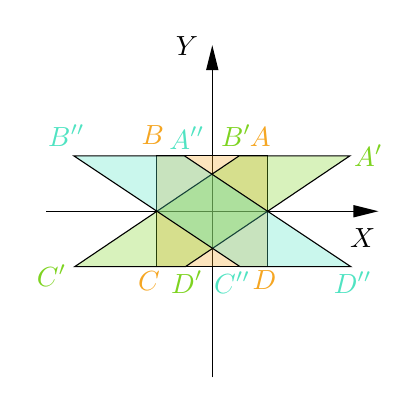
\begin{tikzpicture}[x=0.75pt,y=0.75pt,yscale=-1,xscale=1]
%uncomment if require: \path (0,310); %set diagram left start at 0, and has height of 310

%Straight Lines [id:da258215525060401] 
\draw    (240,240) -- (240,213.33) -- (240,186.67) -- (240,160) -- (240,133.33) -- (240,106.67) -- (240,82) ;
\draw [shift={(240,80)}, rotate = 90] [fill={rgb, 255:red, 0; green, 0; blue, 0 }  ][line width=0.08]  [draw opacity=0] (12,-3) -- (0,0) -- (12,3) -- cycle    ;
%Straight Lines [id:da058671601265665174] 
\draw    (160,160) -- (186.67,160) -- (213.33,160) -- (240,160) -- (266.67,160) -- (293.33,160) -- (318,160) ;
\draw [shift={(320,160)}, rotate = 180] [fill={rgb, 255:red, 0; green, 0; blue, 0 }  ][line width=0.08]  [draw opacity=0] (12,-3) -- (0,0) -- (12,3) -- cycle    ;
%Shape: Rectangle [id:dp4811001215484525] 
\draw  [fill={rgb, 255:red, 245; green, 166; blue, 35 }  ,fill opacity=0.3 ] (213.33,133.33) -- (266.67,133.33) -- (266.67,186.67) -- (213.33,186.67) -- cycle ;
%Shape: Rectangle [id:dp8297367285498773] 
\draw  [fill={rgb, 255:red, 126; green, 211; blue, 33 }  ,fill opacity=0.3 ] (252.91,133.33) -- (306.24,133.33) -- (227.09,186.67) -- (173.76,186.67) -- cycle ;
%Shape: Rectangle [id:dp18591382614366458] 
\draw  [fill={rgb, 255:red, 80; green, 227; blue, 194 }  ,fill opacity=0.3 ] (173.31,133.33) -- (226.64,133.33) -- (306.69,186.67) -- (253.36,186.67) -- cycle ;

% Text Node
\draw (312.88,172.78) node   [align=left] {\begin{minipage}[lt]{9.68pt}\setlength\topsep{0pt}
$\displaystyle X$
\end{minipage}};
% Text Node
\draw (230.8,80.55) node   [align=left] {\begin{minipage}[lt]{12.51pt}\setlength\topsep{0pt}
$\displaystyle Y$
\end{minipage}};
% Text Node
\draw (314.1,133.25) node  [color={rgb, 255:red, 126; green, 211; blue, 33 }  ,opacity=1 ] [align=left] {\begin{minipage}[lt]{8.67pt}\setlength\topsep{0pt}
$\displaystyle A'$
\end{minipage}};
% Text Node
\draw (263.92,124.36) node  [color={rgb, 255:red, 245; green, 166; blue, 35 }  ,opacity=1 ] [align=left] {\begin{minipage}[lt]{8.67pt}\setlength\topsep{0pt}
$\displaystyle A$
\end{minipage}};
% Text Node
\draw (250.01,123.63) node  [color={rgb, 255:red, 126; green, 211; blue, 33 }  ,opacity=1 ] [align=left] {\begin{minipage}[lt]{8.67pt}\setlength\topsep{0pt}
$\displaystyle B'$
\end{minipage}};
% Text Node
\draw (211.71,123.47) node  [color={rgb, 255:red, 245; green, 166; blue, 35 }  ,opacity=1 ] [align=left] {\begin{minipage}[lt]{8.67pt}\setlength\topsep{0pt}
$\displaystyle B$
\end{minipage}};
% Text Node
\draw (161.95,191.14) node  [color={rgb, 255:red, 126; green, 211; blue, 33 }  ,opacity=1 ] [align=left] {\begin{minipage}[lt]{9.68pt}\setlength\topsep{0pt}
$\displaystyle C'$
\end{minipage}};
% Text Node
\draw (210.68,193.75) node  [color={rgb, 255:red, 245; green, 166; blue, 35 }  ,opacity=1 ] [align=left] {\begin{minipage}[lt]{9.68pt}\setlength\topsep{0pt}
$\displaystyle C$
\end{minipage}};
% Text Node
\draw (265.88,193.35) node  [color={rgb, 255:red, 245; green, 166; blue, 35 }  ,opacity=1 ] [align=left] {\begin{minipage}[lt]{9.68pt}\setlength\topsep{0pt}
$\displaystyle D$
\end{minipage}};
% Text Node
\draw (226.68,194.15) node  [color={rgb, 255:red, 126; green, 211; blue, 33 }  ,opacity=1 ] [align=left] {\begin{minipage}[lt]{9.68pt}\setlength\topsep{0pt}
$\displaystyle D'$
\end{minipage}};
% Text Node
\draw (225.12,124.76) node  [color={rgb, 255:red, 80; green, 227; blue, 194 }  ,opacity=1 ] [align=left] {\begin{minipage}[lt]{8.67pt}\setlength\topsep{0pt}
$\displaystyle A''$
\end{minipage}};
% Text Node
\draw (166.72,123.56) node  [color={rgb, 255:red, 80; green, 227; blue, 194 }  ,opacity=1 ] [align=left] {\begin{minipage}[lt]{8.67pt}\setlength\topsep{0pt}
$\displaystyle B''$
\end{minipage}};
% Text Node
\draw (246.72,194.36) node  [color={rgb, 255:red, 80; green, 227; blue, 194 }  ,opacity=1 ] [align=left] {\begin{minipage}[lt]{8.67pt}\setlength\topsep{0pt}
$\displaystyle C''$
\end{minipage}};
% Text Node
\draw (304.32,194.36) node  [color={rgb, 255:red, 80; green, 227; blue, 194 }  ,opacity=1 ] [align=left] {\begin{minipage}[lt]{8.67pt}\setlength\topsep{0pt}
$\displaystyle D''$
\end{minipage}};


\end{tikzpicture}

    }
    \caption{}
    \label{jihebh}
\end{figure}
\section{矩阵的秩}

\subsection{秩的相关不等式证明}

\begin{definition}[满秩方阵]
    对于 $n$ 阶方阵 $\vb*{A}$, 若 $\rank\vb*{A}=n$, 则称 $\vb*{A}$ 为满秩 (非退化) 方阵, 否则称为降秩 (退化) 方阵.
\end{definition}

\begin{theorem}[矩阵与向量组秩的联系]
    设 $\vb*{\alpha}_i~ (i=1,2,\cdots,m),~\vb*{\beta}$ 是 $n$ 维列向量, 则
    $$\rank(\vb*{\alpha}_1,\vb*{\alpha}_2,\cdots,\vb*{\alpha}_m)\leqslant \rank(\vb*{\alpha}_1,\vb*{\alpha}_2,\cdots,\vb*{\alpha}_m,\vb*{\beta})\leqslant \rank(\vb*{\alpha}_1,\vb*{\alpha}_2,\cdots,\vb*{\alpha}_m)+1.$$
\end{theorem}

\begin{example}
    设 $\vb*{A},~\vb*{B}$ 分别是 $f\times m,~f\times n$ 的矩阵, 证明: $\rank\vb*{A}\leqslant \rank(\vb*{A},\vb*{B})\leqslant \rank\vb*{A}+n.$
\end{example}
\begin{proof}{\songti \textbf{证}}
    设 $\vb*{A}=(\vb*{\alpha}_1,\vb*{\alpha}_2,\cdots,\vb*{\alpha}_m),~\vb*{B}=(\vb*{\beta}_1,\vb*{\beta}_2,\cdots,\vb*{\beta}_n)$, 那么 
    $$\rank\vb*{A}=\rank(\vb*{\alpha}_1,\vb*{\alpha}_2,\cdots,\vb*{\alpha}_m)\leqslant \rank(\vb*{\alpha}_1,\vb*{\alpha}_2,\cdots,\vb*{\alpha}_m,\vb*{\beta}_1)\leqslant\cdots\leqslant \rank(\vb*{\alpha}_1,\cdots,\vb*{\alpha}_m,\vb*{\beta}_1,\cdots,\vb*{\beta}_n)=\rank(\vb*{A},\vb*{B})$$
    又因为 
    $$\rank(\vb*{A},\vb*{B})=\rank(\vb*{\alpha}_1,\cdots,\vb*{\alpha}_m,\vb*{\beta}_1,\cdots,\vb*{\beta}_n)\leqslant \rank(\vb*{\alpha}_1,\cdots,\vb*{\alpha}_m,\vb*{\beta}_1,\cdots,\vb*{\beta}_{n-1})+1\leqslant \cdots\leqslant \rank(\vb*{\alpha}_1,\cdots,\vb*{\alpha}_m)+n$$
    综上 $\rank\vb*{A}\leqslant \rank(\vb*{A},\vb*{B})\leqslant \rank\vb*{A}+n$ 成立.
\end{proof}

\begin{theorem}
    对于 $m\times n$ 矩阵 $\vb*{A}$ 与 $\vb*{B}$, 有 $\rank(\vb*{A}+\vb*{B})\leqslant \rank(\vb*{A},\vb*{B})$.
\end{theorem}
\begin{proof}[{\songti \textbf{证}}]
    不妨设 $\vb*{A}=(\vb*{\alpha}_1,\vb*{\alpha}_2,\cdots,\vb*{\alpha}_m),~\vb*{B}=(\vb*{\beta}_1,\vb*{\beta}_2,\cdots,\vb*{\beta}_m)$, 则结论显然成立.
\end{proof}

\begin{theorem}
    对于 $m\times n$ 矩阵 $\vb*{A}$ 与 $m\times s$ 矩阵 $\vb*{B}$, 有 $\rank(\vb*{A},\vb*{B})\leqslant \rank\vb*{A}+\rank\vb*{B}.$
\end{theorem}
\begin{proof}[{\songti \textbf{证}}]
    提示: 用极大无关组可证明.
\end{proof}

\begin{theorem}
    对于 $n$ 阶方阵 $\vb*{A},~\vb*{B}$, 则 $\rank(\vb*{A}\pm\vb*{B})\leqslant \rank\vb*{A}+\rank\vb*{B}.$
\end{theorem}

\begin{theorem}
    对于 $m\times n$ 矩阵 $\vb*{A}$ 与 $n\times s$ 矩阵 $\vb*{B}$, 有 $\rank(\vb*{AB})\leqslant \min\qty{\rank\vb*{A},\rank\vb*{B}}.$
\end{theorem}
\begin{proof}[{\songti \textbf{证}}]
    先设 $\vb*{A}=(\vb*{\alpha}_1,\vb*{\alpha}_2,\cdots,\vb*{\alpha}_n),~\vb*{B}=\mqty(b_{11}&\cdots&b_{1s}\\\vdots&&\vdots\\b_{n1}&\cdots&b_{ns})$, 
    并且无论是 $b_{11}\vb*{\alpha}_1+\cdots+b_{n1}\vb*{\alpha}_n$ 还是 $b_{1s}\vb*{\alpha}_1+\cdots+b_{ns}\vb*{\alpha}_n$, 均可由 $\vb*{\alpha}_1,\cdots,\vb*{\alpha}_n$ 线性表示, 于是
    $$\rank(\vb*{AB})=\rank(b_{11}\vb*{\alpha}_1+\cdots+b_{n1}\vb*{\alpha}_n,\cdots,b_{1s}\vb*{\alpha}_1+\cdots+b_{ns}\vb*{\alpha}_n)\leqslant \rank(\vb*{\alpha}_1,\cdots,\vb*{\alpha}_n)=\rank(\vb*{A})$$
    再设 $\vb*{A}=\mqty(a_{11}&\cdots&a_{1n}\\\vdots&&\vdots\\a_{m1}&\cdots&a_{mn}),~\vb*{B}=\mqty(\vb*{\beta}_1\\ \vdots\\\vb*{\beta}_n)^\top$, 同理 $\rank(\vb*{AB})\leqslant \rank\vb*{B}$, 
    则 $$\rank(\vb*{AB})\leqslant \rank\vb*{A}\text{ 且 }\rank(\vb*{AB})\leqslant \rank\vb*{B}.$$
\end{proof}

\begin{theorem}
    若 $\vb*{A}$ 是 $m\times n$ 矩阵, $\vb*{B}$ 是 $n\times s$ 矩阵, 且 $\vb*{AB}=\vb*{O}$, 则 $\rank\vb*{A}+\rank\vb*{B}\leqslant n.$
\end{theorem}

\begin{theorem}
    对于 $m\times n$ 矩阵 $\vb*{A}$ 与 $s\times t$ 矩阵 $\vb*{B}$, 有 $\rank\mqty(\vb*{A}&\vb*{O}\\\vb*{C}&\vb*{B})\geqslant \rank\vb*{A}+\rank\vb*{B}.$
\end{theorem}

\begin{example}
    设 $\vb*{A},~\vb*{B}$ 为 $n$ 阶方阵, 证明:
    $$\rank(\vb*{AB}-\vb*{E})\leqslant \rank(\vb*{A}-\vb*{E})+\rank(\vb*{B}-\vb*{E})$$
    这里 $\vb*{E}$ 为 $n$ 阶单位矩阵.
\end{example}
\begin{proof}[{\songti \textbf{证}}]
    因为 $\vb*{AB}-\vb*{E}=(\vb*{A}-\vb*{E})\vb*{B}+(\vb*{B}-\vb*{E})$, 于是 
    $$\rank(\vb*{AB}-\vb*{E})\leqslant \rank((\vb*{A}-\vb*{E})\vb*{B})+\rank(\vb*{B}-\vb*{E})\leqslant \rank(\vb*{A}-\vb*{E})+\rank(\vb*{B}-\vb*{E}).$$
\end{proof}

\begin{example}
    设 $\vb*{A},~\vb*{B}$ 为 $n$ 阶方阵, 证明:
    \begin{enumerate}[label=(\arabic{*})]
        \item $\rank(\vb*{A}-\vb*{B})\geqslant \rank\vb*{A}-\rank\vb*{B}$;
        \item 若 $\vb*{A}$ 是可逆矩阵, 则结论 (1) 中的等号成立当且仅当 $\vb*{BA}^{-1}\vb*{B}=\vb*{B}.$
    \end{enumerate}
\end{example}
\begin{proof}[{\songti \textbf{证}}]
    \begin{enumerate}[label=(\arabic{*})]
        \item 由 $\vb*{A}=(\vb*{A}-\vb*{B})+\vb*{B}$, 且 $\rank\vb*{A}\leqslant \rank(\vb*{A}-\vb*{B})+\rank\vb*{B}$, 移项得 $\rank(\vb*{A}-\vb*{B})\geqslant \rank\vb*{A}-\rank\vb*{B}$;
        \item 利用分块矩阵的初等行变换, 得 
        $$\mqty(\vb*{A}-\vb*{B}&\vb*{O}\\\vb*{O}&\vb*{B})\to\mqty(\vb*{A}&\vb*{B}\\\vb*{B}&\vb*{B})\xrightarrow[]{\text{行}}\mqty(\vb*{A}&\vb*{B}\\\vb*{O}&\vb*{B}-\vb*{BA}^{-1}\vb*{B})\xrightarrow[]{\text{列}}\mqty(\vb*{A}&\vb*{O}\\\vb*{O}&\vb*{B}-\vb*{BA}^{-1}\vb*{B})$$
        因为初等行变化不会改变矩阵的秩, 所以 
        $$\rank\mqty(\vb*{A}-\vb*{B}&\vb*{O}\\\vb*{O}&\vb*{B})=\rank\mqty(\vb*{A}&\vb*{O}\\\vb*{O}&\vb*{B}-\vb*{BA}^{-1}\vb*{B})$$
        即
        $$\rank(\vb*{A}-\vb*{B})+\rank\vb*{B}=\rank\vb*{A}+\rank(\vb*{B}-\vb*{BA}^{-1}\vb*{B})$$
        故 $\rank(\vb*{A}-\vb*{B})=\rank\vb*{A}-\rank\vb*{B}$ 当且仅当 $\rank(\vb*{B}-\vb*{BA}^{-1}\vb*{B})=0$, 即 $\vb*{BA}^{-1}\vb*{B}=\vb*{B}.$
    \end{enumerate}
\end{proof}

\begin{example}
    设 $\vb*{A},~\vb*{B}$ 都是数域 $P$ 上的 $n$ 阶方阵, 满足 $\vb*{AB}=\vb*{BA}$, 证明:
    $$\rank(\vb*{A}+\vb*{B})\leqslant \rank\vb*{A}+\rank\vb*{B}-\rank(\vb*{AB}).$$
\end{example}
\begin{proof}[{\songti \textbf{证}}]
    利用分块矩阵的初等行变换, 有
    $$\mqty(\vb*{A}&\vb*{O}\\\vb*{O}&\vb*{B})\xrightarrow[]{\text{行}}\mqty(\vb*{A}&\vb*{B}\\\vb*{O}&\vb*{B})\xrightarrow[]{\text{列}}\mqty(\vb*{A}+\vb*{B}&\vb*{B}\\\vb*{B}&\vb*{B})$$
    因为 $\vb*{AB}=\vb*{BA}$, 于是
    $$\mqty(\vb*{E}&\vb*{O}\\-\vb*{B}&\vb*{A}+\vb*{B})\mqty(\vb*{A}+\vb*{B}&\vb*{B}\\\vb*{B}&\vb*{B})=\mqty(\vb*{A}+\vb*{B}&\vb*{B}\\\vb*{O}&\vb*{AB})$$
    于是, 有 $$\rank\vb*{A}+\rank\vb*{B}=\rank\mqty(\vb*{A}+\vb*{B}&\vb*{B}\\\vb*{B}&\vb*{B})\geqslant \rank\mqty(\vb*{A}+\vb*{B}&\vb*{B}\\\vb*{O}&\vb*{AB})\geqslant \rank(\vb*{A}+\vb*{B})+\rank(\vb*{AB})$$
    即得证不等式.
\end{proof}

\subsection{秩的相关等式证明}

\begin{theorem}
    对于 $m\times n$ 矩阵 $\vb*{A}$ 与 $s\times t$ 矩阵 $\vb*{B}$, 有 $\rank\mqty(\vb*{A}&\vb*{O}\\\vb*{O}&\vb*{B})=\rank\vb*{A}+\rank\vb*{B}.$
\end{theorem}

\begin{theorem}[秩的第一降阶定理]
    若 $\vb*{A}$ 是 $r$ 阶可逆矩阵, 分块矩阵 $\vb*{M}=\mqty(\vb*{A}&\vb*{B}\\\vb*{C}&\vb*{D})$, 那么 $$\rank\vb*{M}=r+\rank(\vb*{D}-\vb*{CA}^{-1}\vb*{B}).$$
\end{theorem}

\begin{example}
    设 $\vb*{A},~\vb*{D}$ 分别为 $m$ 阶与 $n$ 阶可逆矩阵, $\vb*{B},~\vb*{C}$ 分别为 $m\times n$ 与 $n\times m$ 矩阵, 证明:
    $$\rank \vb*{A}-\rank\qty(\vb*{A}-\vb*{BD}^{-1}\vb*{C})=\rank \vb*{D}-\rank\qty(\vb*{D}-\vb*{CA}^{-1}\vb*{B}).$$
\end{example}
\begin{proof}[{\songti \textbf{证}}]
    利用分块矩阵的初等行变换, 得
    \begin{flalign*}
        \mqty(\vb*{A}&\vb*{O}\\\vb*{O}&\vb*{D}-\vb*{CA}^{-1}\vb*{B})&\xrightarrow[]{\text{行}}\mqty(\vb*{A}&\vb*{O}\\\vb*{C}&\vb*{D}-\vb*{CA}^{-1}\vb*{B})\xrightarrow[]{\text{列}}\mqty(\vb*{A}&\vb*{B}\\\vb*{C}&\vb*{D})\\
        \mqty(\vb*{A}-\vb*{BD}^{-1}\vb*{C}&\vb*{O}\\\vb*{O}&\vb*{D})&\xrightarrow[]{\text{行}}\mqty(\vb*{A}-\vb*{BD}^{-1}\vb*{C}&\vb*{B}\\\vb*{O}&\vb*{D})\xrightarrow[]{\text{列}}\mqty(\vb*{A}&\vb*{B}\\\vb*{C}&\vb*{D})
    \end{flalign*}
    因为初等行变化不会改变矩阵的秩, 于是 
    \begin{flalign*}
        \rank\vb*{A}+\rank\qty(\vb*{D}-\vb*{CA}^{-1}\vb*{B})&=\rank\mqty(\vb*{A}&\vb*{O}\\\vb*{O}&\vb*{D}-\vb*{CA}^{-1}\vb*{B})=\rank\mqty(\vb*{A}&\vb*{B}\\\vb*{C}&\vb*{D})\\
        \rank\qty(\vb*{A}-\vb*{BD}^{-1}\vb*{C})+\rank\vb*{D}&=\rank\mqty(\vb*{A}-\vb*{BD}^{-1}\vb*{C}&\vb*{O}\\\vb*{O}&\vb*{D})=\rank\mqty(\vb*{A}&\vb*{B}\\\vb*{C}&\vb*{D})
    \end{flalign*}
    得证 $\rank \vb*{A}-\rank\qty(\vb*{A}-\vb*{BD}^{-1}\vb*{C})=\rank \vb*{D}-\rank\qty(\vb*{D}-\vb*{CA}^{-1}\vb*{B}).$
\end{proof}
\begin{inference}
    \label{rankmn}
    特别地, 令 $\vb*{A}=\lambda_0\vb*{E}_m,~\vb*{D}=\vb*{E}_n$, 其中 $\lambda_0$ 为任意非零常数, 则有
    $$m-\rank\qty(\lambda_0\vb*{E}_m-\vb*{BC})=n-\rank\qty(\lambda_0\vb*{E}_n-\vb*{CB}).$$
\end{inference}

\begin{example}
    设 $\vb*{A}$ 是 $m\times n$ 矩阵, $\vb*{B}$ 是 $n\times s$ 矩阵, 且 $\rank(\vb*{AB})=\rank\vb*{B}$, 证明:
    对任一 $s\times t$ 矩阵 $\vb*{C}$, 有 $\rank(\vb*{ABC})=\rank(\vb*{BC}).$
\end{example}
\begin{proof}[{\songti \textbf{证}}]
    利用分块矩阵的初等行变换, 得 
    $$\mqty(\vb*{ABC}&\vb*{O}\\\vb*{O}&\vb*{B})\xrightarrow[]{\text{行}}\mqty(\vb*{ABC}&\vb*{AB}\\\vb*{O}&\vb*{B})\xrightarrow[]{\text{列}}\mqty(\vb*{O}&\vb*{AB}\\-\vb*{BC}&\vb*{B})\xrightarrow[]{\text{列}}\mqty(\vb*{AB}&\vb*{O}\\\vb*{B}&\vb*{BC})$$
    因为初等行变化不会改变矩阵的秩, 所以
    $$\rank\mqty(\vb*{ABC}&\vb*{O}\\\vb*{O}&\vb*{B})=\rank(\vb*{ABC})+\rank\vb*{B}=\rank\mqty(\vb*{AB}&\vb*{O}\\\vb*{B}&\vb*{BC})\geqslant \rank(\vb*{AB})+\rank(\vb*{BC})$$
    又 $\rank(\vb*{AB})=\rank\vb*{B}$, 所以 $\rank(\vb*{ABC})\geqslant \rank(\vb*{BC})$, 又 $\rank(\vb*{ABC})\leqslant \rank(\vb*{BC})$, 
    故 $$\rank(\vb*{ABC})=\rank(\vb*{BC}).$$
\end{proof}

\subsection{秩的应用}

\begin{example}
    设 $\vb*{A},~\vb*{B}$ 分别是实数域上的 $3\times4$ 和 $4\times3$ 矩阵, 且满足
    $$\vb*{AB}=\mqty(-9&2&2\\-20&5&4\\-35&7&8),~\vb*{BA}=\mqty(-14 &2x-5 &2 &6\\0 &1 &0 &0\\-15 &3x-3 &3 &6\\-32 &6x-7 &4 &14)$$
    求 $x$ 的值.
\end{example}
\begin{solution}
    由推论 \ref{rankmn}, 令 $\lambda_0=1$, 于是  $3-\rank\qty(\vb*{E}_3-\vb*{AB})=4-\rank\qty(\vb*{E}_4-\vb*{BA})$, 那么 
    \begin{flalign*}
        \rank\qty(\vb*{E}_4-\vb*{BA})&=4-3+\rank\qty(\vb*{E}_3-\vb*{AB})\\
        \rank\mqty(15 &5-2x &-2 &-6\\0 &0 &0 &0\\15 &3-3x &-2 &-6\\32 &7-6x &-4 &-13)&=1+\rank\mqty(10 &-2 &-2\\20 &-4 &-4\\35 &-7 &-7)=2
    \end{flalign*}
    解得 $x=-2.$
\end{solution}

\begin{example}
    设 $\vb*{A}$ 是 4 阶矩阵, 向量 $\vb*{\alpha},~\vb*{\beta}$ 是齐次方程组 $(\vb*{A}-\vb*{E})\vb*{x}=\vb*{0}$ 的基础解系, 向量 $\vb*{\gamma}$ 是齐次方程组 $(\vb*{A}+\vb*{E})\vb*{x}=\vb*{0}$ 的基础解系, 求 $\qty(\vb*{A}^2-\vb*{E})\vb*{x}=\vb*{0}$ 的通解
    \begin{tasks}(2)
        \task $c_1\vb*{\alpha}+c_2\vb*{\beta}$ 其中 $c_1,~c_2$ 为任意常数
        \task $c_1\vb*{\alpha}+c_2\vb*{\gamma}$ 其中 $c_1,~c_2$ 为任意常数
        \task $c_1\vb*{\beta}+c_2\vb*{\gamma}$ 其中 $c_1,~c_2$ 为任意常数
        \task $c_1\vb*{\alpha}+c_2\vb*{\beta}+c_3\vb*{\gamma}$ 其中 $c_1,~c_2,~c_3$ 为任意常数
    \end{tasks}
\end{example}
\begin{solution}
    因为向量 $\vb*{\alpha},~\vb*{\beta}$ 是齐次方程组 $(\vb*{A}-\vb*{E})\vb*{x}=\vb*{0}$ 的基础解系, 所以 $$s=n-\rank(\vb*{A}-\vb*{E})\Rightarrow 2=4-\rank(\vb*{A}-\vb*{E})\Rightarrow \rank(\vb*{A}-\vb*{E})=2$$
    同理 $\rank(\vb*{A}+\vb*{E})=3$, 又因为 
    $$\rank\qty(\vb*{A}^2-\vb*{E})=\rank[(\vb*{A}+\vb*{E})(\vb*{A}-\vb*{E})]\leqslant \min\qty{\rank(\vb*{A}+\vb*{E}),\rank(\vb*{A}-\vb*{E})}\Rightarrow \rank\qty(\vb*{A}^2-\vb*{E})\leqslant 2$$
    当 $\rank\qty(\vb*{A}^2-\vb*{E})=0$ 时, $\vb*{A}^2-\vb*{E}=\vb*{O}\Rightarrow (\vb*{A}+\vb*{E})(\vb*{A}-\vb*{E})=\vb*{O}\Rightarrow \rank(\vb*{A}+\vb*{E})+\rank(\vb*{A}-\vb*{E})\leqslant 4$, 而 $\rank(\vb*{A}+\vb*{E})=3,~\rank(\vb*{A}-\vb*{E})=2$, 与之矛盾;
    当 $\rank\qty(\vb*{A}^2-\vb*{E})=2$ 时, 说明有 2 个线性无关解, $\qty(\vb*{A}^2-\vb*{E})\vb*{x}=\vb*{0}\Rightarrow (\vb*{A}+\vb*{E})(\vb*{A}-\vb*{E})\vb*{x}=\vb*{0}$, 即 $\vb*{\alpha},~\vb*{\beta},~\vb*{\gamma}$ 是方程组的三个解, 
    又因为 $\vb*{\alpha},~\vb*{\beta}$ 是齐次方程组 $(\vb*{A}-\vb*{E})\vb*{x}=\vb*{0}$ 的基础解系, 说明 $\vb*{\alpha},~\vb*{\beta}$ 线性无关, 且 $\vb*{\alpha},~\vb*{\beta}$ 是特征值 1 对应的特征向量, $\vb*{\gamma}$ 是 -1 对应的特征向量, 因此 $\vb*{\gamma}$ 与 $\vb*{\alpha}$ 或 $\vb*{\gamma}$ 线性无关, 故方程组有 3 个线性无关解, 矛盾;
    所以 $\rank\qty(\vb*{A}^2-\vb*{E})=1\Rightarrow s'=n-\rank\qty(\vb*{A}^2-\vb*{E})=4-1=3$, 因此选 D.
\end{solution}

\section{矩阵的等价标准形}

% \subsection{等价标准形}
% 
% \begin{example}
%     设 $\vb*{A}=\mqty(1&2&3\\2&1&2\\3&3&5\\1&-1&-1\\4&2&4)$, 求可逆矩阵 $\vb*{P},~\vb*{Q}$ 使 $\vb*{PAQ}$ 为 $\vb*{A}$ 的等价标准形.
% \end{example}
% \begin{solution}
%     由矩阵的初等变换, 
%     \begin{flalign*}
%         \mqty(\vb*{A} & \vb*{E}_5 \\\vb*{E}_3&\vb*{O})=\left(\begin{array}{c:c}
%                 \begin{matrix}
%                     1 & 2  & 3  \\
%                     2 & 1  & 2  \\
%                     3 & 3  & 5  \\
%                     1 & -1 & -1 \\
%                     4 & 2  & 4
%                 \end{matrix} & \vb*{E}_5 \\ \hdashline
%                 \vb*{E}_3      & \vb*{O}
%             \end{array}\right)=
%     \end{flalign*}
% \end{solution}

\subsection{矩阵分解}

\begin{example}
    设 $\vb*{A}$ 是 $n$ 阶方阵, 证明: 存在一 $n$ 阶可逆矩阵 $\vb*{B}$ 及一个 $n$ 阶等幂矩阵 $\vb*{C}$, 使得 $\vb*{A}=\vb*{BC}.$
\end{example}
\begin{proof}[{\songti \textbf{证}}]
    设 $\rank\vb*{A}=r$, 则存在 $n$ 阶可逆矩阵 $\vb*{P}$ 和 $\vb*{Q}$ 使得, 
    $$\vb*{A}=\vb*{P}\mqty(\vb*{E}_r&\vb*{O}\\\vb*{O}&\vb*{O})\vb*{Q}=(\vb*{PQ})\vb*{Q}^{-1}\mqty(\vb*{E}_r&\vb*{O}\\\vb*{O}&\vb*{O})\vb*{Q}$$
    令 $\vb*{B}=\vb*{PQ},~\vb*{C}=\vb*{Q}^{-1}\mqty(\vb*{E}_r&\vb*{O}\\\vb*{O}&\vb*{O})\vb*{Q}$, 并且
    $$\vb*{C}^2=\vb*{Q}^{-1}\mqty(\vb*{E}_r&\vb*{O}\\\vb*{O}&\vb*{O})\vb*{Q}\vb*{Q}^{-1}\mqty(\vb*{E}_r&\vb*{O}\\\vb*{O}&\vb*{O})\vb*{Q}=C$$
    故得证.
\end{proof}

\begin{example}
    一个矩阵称为行 (列) 满秩矩阵, 如果它的行 (列) 向量组是线性无关的, 
    \begin{enumerate}[label=(\arabic{*})]
        \item 证明: 如果一个 $m\times n$ 矩阵 $\vb*{A}$ 的秩为 $r$, 那么有 $m\times r$ 的列满秩矩阵 $\vb*{B}$ 和 $r\times n$ 的行满秩矩阵 $\vb*{C}$, 使得 $\vb*{A}=\vb*{BC}$, 我们称 $\vb*{A}=\vb*{BC}$ 为矩阵 $\vb*{A}$ 的满秩分解表达式;
        \item 利用 (1) 求矩阵 $\vb*{A}=\mqty(1&2&0&1&1&10\\3&6&1&4&2&36\\2&4&0&2&2&27\\6&12&1&7&5&73)$ 的满秩分解表达式.
    \end{enumerate}
\end{example}
\begin{solution}
    \begin{enumerate}[label=(\arabic{*})]
        \item 因为 $\rank \vb*{A}=r$, 所以存在 $m$ 阶可逆矩阵 $\vb*{P}$ 和 $n$ 阶可逆矩阵 $\vb*{Q}$, 使得
              $$\vb*{A}=\vb*{P}\mqty(\vb*{E}_r&\vb*{O}\\\vb*{O}&\vb*{O})\vb*{Q}=\vb*{P}\mqty(\vb*{E}_r\\\vb*{O})(\vb*{E}_r,\vb*{O})\vb*{Q}$$
              令 $\vb*{B}=\vb*{P}\mqty(\vb*{E}_r\\\vb*{O}),~\vb*{C}=(\vb*{E}_r,\vb*{O})\vb*{Q}$, 则 $\vb*{B}$ 是 $m\times r$ 的列满秩矩阵, $\vb*{C}$ 是 $r\times n$ 的行满秩矩阵, 且 $\vb*{A}=\vb*{BC}.$
        \item 用初等行变换和初等列变换将矩阵 $\vb*{A}$ 化为等价标准形, 然后求逆即可, 具体地, 有
              \begin{flalign*}
                  \vb*{A} & \xrightarrow[\substack{r_3-2r_1 \\r_4-6r_1}]{r_2-3r_1}\mqty(1&2&0&1&1&10\\0&0&1&1&-1&6\\0&0&0&0&0&7\\0&0&1&1&-1&13)\xrightarrow[\substack{r_4-r_3\\r_3\times\frac{1}{7}}]{r_4-r_2}\mqty(1&2&0&1&1&10\\0&0&1&1&-1&6\\0&0&0&0&0&1\\0&0&0&0&0&0)\\
                          & \xrightarrow[\substack{c_5-c_1  \\c_6-10c_1}]{\substack{c_2-2c_1\\c_4-c_1}}\mqty(1&0&0&0&0&0\\0&0&1&1&-1&6\\0&0&0&0&0&1\\0&0&0&0&0&0)\xrightarrow[\substack{c_5+c_3\\c_6-6c_3}]{c_4-c_3}\mqty(1&0&0&0&0&0\\0&0&1&0&0&0\\0&0&0&0&0&1\\0&0&0&0&0&0)\xrightarrow[c_3\leftrightarrow c_6]{c_2\leftrightarrow c_3}\mqty(\vb*{E}_3&\vb*{O}\\\vb*{O}&\vb*{O})_{4\times6}
              \end{flalign*}
              用矩阵表示为
              $$\vb*{L}_4\vb*{L}_3\vb*{L}_2\vb*{L}_1\vb*{A}\vb*{R}_1\vb*{R}_2\vb*{E}_{23}\vb*{E}_{36}=\mqty(\vb*{E}_3&\vb*{O}\\\vb*{O}&\vb*{O})_{4\times6}$$
              其中 $$\vb*{L}_1=\mqty(1\\-3&1\\-2&&1\\-6&&&1),\vb*{L}_2=\mqty(1\\&1\\&&1\\&-1&&1),\vb*{L}_3=\mqty(1\\&1\\&&1\\&&-1&1),\vb*{L}_4=\mqty(1\\&1\\&&\dfrac{1}{7}\\&&&1)$$
              $$\vb*{R}_1=\mqty(1&-2&0&-1&-1&-10\\&1\\&&1\\&&&1\\&&&&1\\&&&&&1),~\vb*{R}_2=\mqty(1\\&1\\&&1&-1&1&-6\\&&&1\\&&&&1\\&&&&&1)$$
              % $$\vb*{E}_{23}=\mqty(\dmat{1\\&&1\\&1,1,1,1}) ,~\vb*{E}_{36}=\mqty(1\\&1\\&&&&&1\\&&&1\\&&&&1\\&&1)$$
              于是, 有 $$\vb*{A}=\qty(\vb*{L}_1^{-1}\vb*{L}_2^{-1}\vb*{L}_3^{-1}\vb*{L}_4^{-1}\mqty(\vb*{E}_3\\\vb*{O}))\qty(\mqty(\vb*{E}_3,\vb*{O})\vb*{E}_{36}\vb*{E}_{23}\vb*{R}_2^{-1}\vb*{R}_1^{-1})=\vb*{BC}$$
              那么 $$\vb*{B}=\vb*{L}_1^{-1}\vb*{L}_2^{-1}\vb*{L}_3^{-1}\vb*{L}_4^{-1}\mqty(\vb*{E}_3\\\vb*{O})=\mqty(1&0&0\\3&1&0\\2&0&7\\6&1&7)$$
              $$\vb*{C}=\mqty(\vb*{E}_3,\vb*{O})\vb*{E}_{36}\vb*{E}_{23}\vb*{R}_2^{-1}\vb*{R}_1^{-1}=\mqty(1&2&0&1&1&10\\0&0&1&1&-1&6\\0&0&0&0&0&1).$$
    \end{enumerate}
\end{solution}

\subsection{矩阵方程}

\begin{example}
    设矩阵 $\vb*{A}=\mqty(1&1&-1\\-1&1&1\\1&-1&1)$, 其伴随矩阵记作 $\vb*{A}^*$, 求满足
    $$\vb*{A}^*\vb*{X}\qty(\dfrac{1}{2}\vb*{A}^*)^*=8\vb*{A}^{-1}\vb*{X}+4\vb*{E}$$ 的矩阵 $\vb*{X}.$
\end{example}
\begin{solution}
    $\det \vb*{A}=\mqty|1&1&-1\\-1&1&1\\1&-1&1|=4$, 且 $\vb*{A}\vb*{A}^*=|\vb*{A}|\vb*{E}=4\vb*{E}$, 于是给矩阵方程同时左乘 $\vb*{A}$, 得
    \begin{flalign*}
        \vb*{A}\vb*{A}^*\vb*{X}\qty(\dfrac{1}{2}\vb*{A}^*)^* =8\vb*{A}\vb*{A}^{-1}\vb*{X}+4\vb*{A}\vb*{E} \Rightarrow4\vb*{E}\vb*{X}\qty(\dfrac{1}{2}\vb*{A}^*)^*=8\vb*{E}\vb*{X}+4\vb*{A}\vb*{E} \Rightarrow\vb*{X}\qty(\dfrac{1}{2}\vb*{A}^*)^*                 =2\vb*{X}+\vb*{A}
    \end{flalign*}
    并且 $\qty(\dfrac{1}{2}\vb*{A}^*)^*=\qty(\dfrac{1}{2})^{3-1}\qty(\vb*{A}^*)^*=\dfrac{1}{4}\qty|\vb*{A}^*|^*=\dfrac{1}{4}|\vb*{A}|^{3-2}\vb*{A}=\vb*{A}$, 以及 $\det(\vb*{A}-2\vb*{E})= -4\neq0$, 于是 $\vb*{A}-2\vb*{E}$ 可逆, 
    而 $(\vb*{A}-2\vb*{E})^{-1}=\mqty(-1&1&-1\\-1&-1&1\\1&-1&-1)^{-1}=-\dfrac{1}{2}\mqty(1&1&0\\0&1&1\\1&0&1)$, 那么
    $$\vb*{X}=-\dfrac{1}{2}\mqty(1&1&-1\\-1&1&1\\1&-1&1)\mqty(1&1&0\\0&1&1\\1&0&1)=\mqty(0&-1&0\\0&0&-1\\-1&0&0).$$
\end{solution}

\begin{example}
    $\vb*{A},~\vb*{B}$ 是数域 $K$ 上的 $n$ 阶已知方阵, $\det \vb*{A}=\dfrac{1}{2},~\det\vb*{B}=\dfrac{1}{3}$, 求解关于 $\vb*{X}$ 的矩阵方程
    $$\vb*{X}+\qty(\qty(\vb*{A}^\top\vb*{B})^*\vb*{A}^\top)^{-1}+\vb*{BA}^{-1}\vb*{B}=\vb*{X}\qty(\vb*{B}^\top\qty(\vb*{AB}^\top)^{-1}\vb*{A}^2)^{-1}(\vb*{A}+2\vb*{B}).$$
\end{example}
\begin{solution}
    注意到 $\qty(\vb*{A}^\top\vb*{B})^*=\qty|\vb*{A}^\top\vb*{B}|\qty(\vb*{A}^\top\vb*{B})^{-1}=\qty|\vb*{A}^\top\vb*{B}|\vb*{B}^{-1}\qty(\vb*{A}^\top)^{-1}$, 
    那么 $$\qty(\qty(\vb*{A}^\top\vb*{B})^*\vb*{A}^\top)^{-1}=\qty(\qty|\vb*{A}^\top\vb*{B}|\vb*{B}^{-1}\vb*{E})^{-1}=\dfrac{1}{\qty|\vb*{A}^\top\vb*{B}|}\vb*{B}=6\vb*{B}$$
    并且 $\qty(\vb*{B}^\top\qty(\vb*{AB}^\top)^{-1}\vb*{A}^2)^{-1}=\qty(\vb*{B}^\top\qty(\vb*{B}^\top)^{-1}\vb*{A}^{-1}\vb*{A}^2)^{-1}=\vb*{A}^{-1}$, 于是
    $$\vb*{X}\qty(\vb*{B}^\top\qty(\vb*{AB}^\top)^{-1}\vb*{A}^2)^{-1}(\vb*{A}+2\vb*{B})=\vb*{X}\vb*{A}^{-1}\qty(\vb*{A}+2\vb*{B})=\vb*{X}+2\vb*{XA}^{-1}\vb*{B}$$
    那么 \begin{flalign*}
        \vb*{X}=\dfrac{1}{2}\qty(6\vb*{B}+\vb*{BA}^{-1}\vb*{B})\qty(\vb*{A}^{-1}\vb*{B})^{-1}=\dfrac{1}{2}\qty(6\vb*{B}+\vb*{BA}^{-1}\vb*{B})\qty(\vb*{B}^{-1}\vb*{A})=3\vb*{A}+\dfrac{1}{2}\vb*{B}
    \end{flalign*}
\end{solution}

\begin{example}[2016 浙江大学]
    设矩阵 $\vb*{A}=\begin{pmatrix}
            a & b & c \\
            d & e & f \\
            h & x & y
        \end{pmatrix}$ 的逆矩阵 $\vb*{A}^{-1}=\begin{pmatrix}
            -1 & -2 & -1 \\
            -2 & 1  & 0  \\
            0  & -3 & 1
        \end{pmatrix}$, 矩阵 $\vb*{B}=\begin{pmatrix}
            a-2b & b-3  & -c \\
            d-2e & e-3f & -f \\
            h-2x & x-3y & -y
        \end{pmatrix}$, 求矩阵 $\vb*{X}$ 使之满足
    $$\vb*{X}+\qty(\vb*{B}\qty(\vb*{A}^{\top}\vb*{B}^2)^{-1}\vb*{A}^{\top})^{-1}=\vb*{X}\qty(\vb*{A}^2\qty(\vb*{B}^{\top}\vb*{A})^{-1}\vb*{B}^{\top})^{-1}(\vb*{A}+\vb*{B}).$$
\end{example}
\begin{solution}
    先证 $\vb*{B}$ 是可逆矩阵, 为此, 对行列式 $|\vb*{B}|$ 依次将第 2 列减去第 3 列的 3 倍, 第 1 列加上第 2 列的 2 倍, 再按第 1 行拆项, 得
    \begin{flalign*}
        |\vb*{B}| & =\begin{vmatrix}
                         a-2b & b-3  & -c \\
                         d-2e & e-3f & -f \\
                         h-2x & x-3y & -y
                     \end{vmatrix}\xlongequal[c_1+2c_2]{c_2-3c_3}\begin{vmatrix}
                                                                     a+6c-6 & b+3c-3 & -c \\
                                                                     d      & e      & -f \\
                                                                     h      & x      & -y
                                                                 \end{vmatrix}=-|\vb*{A}|+3(c-1)\begin{vmatrix}
                                                                                                    2 & 1 & 0  \\
                                                                                                    d & e & -f \\
                                                                                                    h & x & -y
                                                                                                \end{vmatrix} \\
                  & =1-3(c-1)(2A_{11}-A_{12})
    \end{flalign*}
    其中 $A_{11},~A_{12}$ 是矩阵 $\vb*{A}$ 的第 1 行的前两个元素的代数余子式, 另一方面, 易知 $|\vb*{A}^{-1}|=-1$, 所以 $|\vb*{A}|=-1$, 于是, 有
    $\vb*{A}^*=|\vb*{A}|\vb*{A}^{-1}=\mqty(1&2&1\\2&-1&0\\0&3&1)$, 由此可知 $A_{11}=1,~A_{12}=2$, 于是 $|\vb*{B}|=1$, 表明 $\vb*{B}$ 是可逆矩阵, 因此
    $$\qty(\vb*{B}\qty(\vb*{A}^{\top}\vb*{B}^2)^{-1}\vb*{A}^{\top})^{-1}=\vb*{B},~\vb*{X}\qty(\vb*{A}^2\qty(\vb*{B}^{\top}\vb*{A})^{-1}\vb*{B}^{\top})^{-1}=\vb*{A}^{-1}$$
    故原方程可化简为 $\vb*{X}+\vb*{B}=\vb*{XA}^{-1}(\vb*{A}+\vb*{B})\Rightarrow \vb*{X}(\vb*{A}^{-1}\vb*{B})=\vb*{B}$, 所以
    $$\vb*{X}=\vb*{B}(\vb*{A}^{-1}\vb*{B})^{-1}=\vb*{A}.$$
\end{solution}

\begin{example}
    设矩阵 $\vb*{A}=\begin{pmatrix}
            1 & -1 & 0  & 0  \\
            0 & 1  & -1 & 0  \\
            0 & 0  & 1  & -1 \\
            0 & 0  & 0  & 1
        \end{pmatrix}$, $\vb*{B}=\begin{pmatrix}
            2 & 1 & 3 & 4 \\
            0 & 2 & 1 & 3 \\
            0 & 0 & 2 & 1 \\
            0 & 0 & 0 & 2
        \end{pmatrix}$, 求解方程
    $$\vb*{X}\qty(\vb*{E}_n-\vb*{B}^{-1}\vb*{A})^{\top}\vb*{B}^{\top}=\vb*{E}_n.$$
\end{example}
\begin{solution}
    $\vb*{E}_n=\vb*{X}\qty(\vb*{B}\qty(\vb*{E}_n-\vb*{B}^{-1}\vb*{A}))^{\top}=\vb*{X}\qty(\vb*{BE}_n-\vb*{BB}^{-1}\vb*{A})^{\top}=\vb*{X}\qty(\vb*{B}-\vb*{A})^{\top}\Rightarrow \vb*{X}=\qty(\qty(\vb*{B}-\vb*{A})^{\top})^{-1}$, 
    \begin{flalign*}
        \vb*{X} & =\qty(\qty(\begin{pmatrix}
                                 2 & 1 & 3 & 4 \\
                                 0 & 2 & 1 & 3 \\
                                 0 & 0 & 2 & 1 \\
                                 0 & 0 & 0 & 2
                             \end{pmatrix}-\begin{pmatrix}
                                               1 & -1 & 0  & 0  \\
                                               0 & 1  & -1 & 0  \\
                                               0 & 0  & 1  & -1 \\
                                               0 & 0  & 0  & 1
                                           \end{pmatrix})^{\top})^{-1}
        =\begin{pNiceArray}{cc:cc}
             1 & 0 & 0 & 0 \\
             2 & 1 & 0 & 0 \\ \hdottedline
             3 & 2 & 1 & 0 \\
             4 & 3 & 2 & 1
         \end{pNiceArray}^{-1}                                                                                                         \\
                & =\begin{pNiceArray}{c:c}
                       \begin{pmatrix}
                1 & 0 \\
                2 & 1
            \end{pmatrix}^{-1}                & O                                   \\ \hdottedline
                       -\begin{pmatrix}
                1 & 0 \\
                2 & 1
            \end{pmatrix}^{-1}\begin{pmatrix}
                3 & 2 \\
                4 & 3
            \end{pmatrix}\begin{pmatrix}
                1 & 0 \\
                2 & 1
            \end{pmatrix}^{-1} & \begin{pmatrix}
                1 & 0 \\
                2 & 1
            \end{pmatrix}^{-1}
                   \end{pNiceArray}=\begin{pmatrix}
                                        1  & 0  & 0  & 0 \\
                                        -2 & 1  & 0  & 0 \\
                                        1  & -2 & 1  & 0 \\
                                        0  & 1  & -2 & 1
                                    \end{pmatrix}.
    \end{flalign*}
\end{solution}

\begin{example}
    设 $\vb*{A}=\mqty(1& 2& 2\\ 2& 5& 4\\ 2& 4& 5),~\vb*{B}=\mqty(1&1\\1&0),~\vb*{C}=\begin{pmatrix}
            1 & 1 &   &   &   \\
              & 1 & 1 &   &   \\
              &   & 1 & 1 &   \\
              &   &   & 1 & 1 \\
              &   &   &   & 1
        \end{pmatrix}$, 求 $\vb*{X}$ 使 $\vb*{X}\mqty(\vb*{O}&\vb*{B}\\\vb*{A}&\vb*{O})=\vb*{C}.$
\end{example}
\begin{solution}
    易得 $\vb*{A},~\vb*{B}$ 都可逆, 且 $\mqty(\vb*{O}&\vb*{B}\\\vb*{A}&\vb*{O})^{-1}=\mqty(\vb*{O}&\vb*{A}^{-1}\\\vb*{B}^{-1}&\vb*{O})$, 所以 $\vb*{X}=\vb*{C}\mqty(\vb*{O}&\vb*{A}^{-1}\\\vb*{B}^{-1}&\vb*{O})$, 且
    $$\vb*{C}=\begin{pNiceArray}{ccc:cc}
            1 & 1 &   &   &   \\
            & 1 & 1 &   &   \\
            &   & 1 & 1 &   \\ \hdottedline
            &   &   & 1 & 1 \\
            &   &   &   & 1
        \end{pNiceArray}=\begin{pNiceArray}{ccc:cc}
            1 & 1 & 0 & 0 & 0 \\
            0 & 1 & 1 & 0 & 0 \\
            0 & 0 & 1 & 1 & 0 \\ \hdottedline
            0 & 0 & 0 & 1 & 1 \\
            0 & 0 & 0 & 0 & 1
        \end{pNiceArray}=\mqty(\vb*{C}_1&\vb*{C}_2\\\vb*{O}&\vb*{C}_3)$$
    并且 $\vb*{A}^{-1}=\mqty(9& -2& -2 \\-2& 1& 0 \\-2& 0& 1),~\vb*{B}^{-1}=\mqty(1& -1\\0& 1)$, 那么
    $$\vb*{X}=\mqty(\vb*{C}_2\vb*{B}^{-1}& \vb*{C}_1\vb*{A}^{-1}\\\vb*{C}_3\vb*{B}^{-1}&\vb*{O})=\begin{pNiceArray}{cc:ccc}
            0 & 0  & 7  & -1 & -2 \\
            0 & 0  & -4 & 1  & 1  \\
            1 & -1 & -2 & 0  & 1  \\ \hdottedline
            1 & 0  & 0  & 0  & 0  \\
            0 & 1  & 0  & 0  & 0
        \end{pNiceArray}.$$
\end{solution}

\begin{example}
    设 4 阶矩阵 $\vb*{A}$ 的伴随矩阵 $\vb*{A}^*=\begin{pmatrix}
            1 & 0  & 0 & 0 \\
            0 & 1  & 0 & 0 \\
            1 & 0  & 1 & 0 \\
            0 & -3 & 0 & 8
        \end{pmatrix}$, 求解矩阵方程 $\vb*{AXA}^{-1}=\vb*{XA}^{-1}+3\vb*{E}_4$, 并计算 $\vb*{X}^*\vb*{A}.$
\end{example}
\begin{solution}
    同例题 \ref{ABA} 的解法, 解得 $\vb*{X}=\begin{pmatrix}
            6 & 0 & 0 & 0  \\
            0 & 6 & 0 & 0  \\
            6 & 0 & 6 & 0  \\
            0 & 3 & 0 & -1
        \end{pmatrix}$, 由于 $$\vb*{X}^*\vb*{A}=\vb*{X}^*\dfrac{1}{|\vb*{A}|^{4-2}}\qty(\vb*{A}^*)^*=\dfrac{1}{4}\vb*{X}^*\qty(\vb*{A}^*)^*=\dfrac{1}{4}\qty(\vb*{A}^*\vb*{X})^*$$
    \begin{flalign*}
        \vb*{X}^*\vb*{A} & =\dfrac{1}{4}\qty(\begin{pmatrix}
                                                     1 & 0  & 0 & 0 \\
                                                     0 & 1  & 0 & 0 \\
                                                     1 & 0  & 1 & 0 \\
                                                     0 & -3 & 0 & 8
                                                 \end{pmatrix}\begin{pmatrix}
                                                                  6 & 0 & 0 & 0  \\
                                                                  0 & 6 & 0 & 0  \\
                                                                  6 & 0 & 6 & 0  \\
                                                                  0 & 3 & 0 & -1
                                                              \end{pmatrix})^*=\dfrac{1}{4}\begin{pNiceArray}{cc:cc}
                                                                                           6  & 0 & 0 & 0  \\
                                                                                           0  & 6 & 0 & 0  \\ \hdottedline
                                                                                           12 & 0 & 6 & 0  \\
                                                                                           0  & 6 & 0 & -8 \\
                                                                                       \end{pNiceArray}^*            \\
                         & =\begin{pNiceArray}{c:c}
                                \begin{vmatrix}
                6 & 0  \\
                0 & -8
            \end{vmatrix}\begin{pmatrix}
                6 & 0 \\
                0 & 6
            \end{pmatrix}^* & O                            \\ \hdottedline
                                -\begin{pmatrix}
                6 & 0  \\
                0 & -8
            \end{pmatrix}^*\begin{pmatrix}
                12 & 0 \\
                0  & 6
            \end{pmatrix}\begin{pmatrix}
                6 & 0 \\
                0 & 6
            \end{pmatrix}^*
                                & \begin{vmatrix}
                6 & 0 \\
                0 & 6
            \end{vmatrix}\begin{pmatrix}
                6 & 0  \\
                0 & -8
            \end{pmatrix}^*
                            \end{pNiceArray}=\begin{pmatrix}
                                                 -72 & 0   & 0   & 0  \\
                                                 0   & -72 & 0   & 0  \\
                                                 144 & 0   & -72 & 0  \\
                                                 0   & -54 & 0   & 54
                                             \end{pmatrix}.
    \end{flalign*}
\end{solution}

\begin{example}
    设 $4$ 阶矩阵 $\vb*{A}=\begin{pmatrix}
            1 & 2 & 0  & 0 \\
            1 & 3 & 0  & 0 \\
            0 & 0 & 0  & 2 \\
            0 & 0 & -1 & 0
        \end{pmatrix}$, 求解 $\qty[\qty(\dfrac{1}{2}\vb*{A})^*]^{-1}\vb*{XA}^{-1}=2\vb*{AX}+12\vb*{E}_4.$
\end{example}
\begin{solution}
    因为 $|\vb*{A}|=\begin{vmatrix}
            1 & 2 \\
            1 & 3
        \end{vmatrix}
        \begin{vmatrix}
            0  & 2 \\
            -1 & 0
        \end{vmatrix}=2$, $\qty[\qty(\dfrac{1}{2}\vb*{A})^*]^{-1}=\qty[\qty|\dfrac{1}{2}\vb*{A}|\qty(\dfrac{1}{2}\vb*{A})^{-1}]^{-1}=8\cdot \dfrac{1}{2}\vb*{A}=4\vb*{A}$, 
    因此原方程变成 $$4\vb*{AXA}^{-1}=2\vb*{AX}+12\vb*{E}_4\Rightarrow 2\vb*{AXA}^{-1}=\vb*{AX}+6\vb*{E}_4\Rightarrow \vb*{X}=6\vb*{A}^{-1}\qty(2\vb*{A}^{-1}-\vb*{E}_4)^{-1}=6\qty(2\vb*{E}_4-\vb*{A})^{-1}$$
    \begin{flalign*}
        \vb*{X} & =6\qty(\begin{pmatrix}
                             2 &   &   &   \\
                               & 2 &   &   \\
                               &   & 2 &   \\
                               &   &   & 2
                         \end{pmatrix}-\begin{pmatrix}
                                           1 & 2 & 0  & 0 \\
                                           1 & 3 & 0  & 0 \\
                                           0 & 0 & 0  & 2 \\
                                           0 & 0 & -1 & 0
                                       \end{pmatrix})^{-1}=6\begin{pNiceArray}{cc:cc}
                                                                1  & -2 & 0 & 0  \\
                                                                -1 & -1 & 0 & 0  \\ \hdottedline
                                                                0  & 0  & 2 & -2 \\
                                                                0  & 0  & 1 & 2
                                                            \end{pNiceArray}^{-1}                                     \\
                & =6\begin{pNiceArray}{c:c}
                        \begin{pmatrix}
                1  & -2 \\
                -1 & -1
            \end{pmatrix}^{-1} & O                  \\ \hdottedline
                        O                  & \begin{pmatrix}
                2 & -2 \\
                1 & 2
            \end{pmatrix}^{-1}
                    \end{pNiceArray}=6\begin{pNiceArray}{c:c}
                                          -\dfrac{1}{3} \begin{pmatrix}
                -1 & 2 \\
                1  & 1
            \end{pmatrix} & O                             \\ \hdottedline
                                          O                             & \dfrac{1}{6} \begin{pmatrix}
                2  & 2 \\
                -1 & 2
            \end{pmatrix}
                                      \end{pNiceArray} \\
                & =\begin{pNiceArray}{c:c}
                       -2 \begin{pmatrix}
                -1 & 2 \\
                1  & 1
            \end{pmatrix} & O                \\ \hdottedline
                       O                  & \begin{pmatrix}
                2  & 2 \\
                -1 & 2
            \end{pmatrix}
                   \end{pNiceArray}=\begin{pmatrix}
                                        2  & -4 & 0  & 0 \\
                                        -2 & -2 & 0  & 0 \\
                                        0  & 0  & 2  & 2 \\
                                        0  & 0  & -1 & 2
                                    \end{pmatrix}.
    \end{flalign*}
\end{solution}



\chapter{线性方程组}%============================11

\begin{flushright}
    \begin{tabular}{r||}
        \textit{“我们的知识只是一种影像, 而不是事物本身. ”}\\
        ——\textit{施密特}
    \end{tabular}
\end{flushright}

在线性代数中, 向量是一个基本的概念, 它可以用来表示空间中的方向和大小. 向量可以是几何向量 (有大小和方向) 或者抽象向量 (只有方向). 下面是一些关于向量的基本概念和性质: 

1. 向量的表示: 向量通常用箭头表示或黑体小写字母, 例如 $\vec{v}$. 在二维空间中, 向量可以表示为 $\vec{v} = \begin{pmatrix} v_1 \\ v_2 \end{pmatrix}$, 其中 $v_1$ 和 $v_2$ 分别是向量在x轴和y轴上的分量. 在三维空间中, 向量可以表示为 $\vec{v} = \begin{pmatrix} v_1 \\ v_2 \\ v_3 \end{pmatrix}$. 

2. 向量的运算: 向量之间可以进行加法和数乘运算. 向量的加法是指将两个向量的对应分量相加, 数乘是指一个向量乘以一个标量, 即将向量的每个分量乘以该标量. 

3. 向量的模长: 向量的模长是指向量的大小, 通常表示为 $||\vec{v}||$ 或 $|\vec{v}|$. 在二维空间中, 向量 $\vec{v} = \begin{pmatrix} v_1 \\ v_2 \end{pmatrix}$ 的模长为 $||\vec{v}|| = \sqrt{v_1^2 + v_2^2}$. 

4. 向量的点积: 向量的点积(内积)是一种重要的向量运算, 定义为两个向量对应分量相乘后再相加的结果, 记为 $\vec{v} \cdot \vec{w}$. 如果 $\vec{v} = \begin{pmatrix} v_1 \\ v_2 \end{pmatrix}$, $\vec{w} = \begin{pmatrix} w_1 \\ w_2 \end{pmatrix}$, 则 $\vec{v} \cdot \vec{w} = v_1w_1 + v_2w_2$. 

5. 向量的叉积: 向量的叉积(外积)是二维或三维向量特有的运算, 结果是一个新的向量. 在三维空间中, 如果 $\vec{v} = \begin{pmatrix} v_1 \\ v_2 \\ v_3 \end{pmatrix}$, $\vec{w} = \begin{pmatrix} w_1 \\ w_2 \\ w_3 \end{pmatrix}$, 则 $\vec{v} \times \vec{w} = \begin{pmatrix} v_2w_3 - v_3w_2 \\ v_3w_1 - v_1w_3 \\ v_1w_2 - v_2w_1 \end{pmatrix}$. 

向量在几何、物理和工程等领域有着广泛的应用, 是线性代数中的重要概念. 通过对向量的运算和性质的理解, 我们可以更好地处理空间中的问题, 并解决各种复杂的计算和分析. 

\section{向量的运算}

\subsection{向量的定义}

\begin{definition}[向量的定义]
    由 $ n $ 个数 $ a_{1}, a_{2}, \cdots, a_{n} $ 组成的有序数组称为 $ n $ 维向量, 简称\textit{向量}.
    $$\vb*{\alpha}=\left(a_{1}, a_{2}, \cdots, a_{n}\right)$$
    称为 $ n $ 维行向量, $ a_{i} $ 称为 $ \vb*{\alpha} $ 的第 $ i $ 个分量.
    $$\vb*{\beta}=\mqty(b_{1} \\
        b_{2} \\
        \vdots \\
        b_{n})=\left(b_{1}, b_{2}, \cdots, b_{n}\right)^{\mathrm{T}}$$
    称为 $ n $ 维列向量.
    由定义可以看出, $ n $ 维行 (列) 向量就是 $ 1 \times n(n \times 1) $ 矩阵.
\end{definition}

\begin{definition}[零向量与负向量]
    分量全为 $0$ 的向量称为\textit{零向量}; 设 $ \vb*{\alpha}=\left(a_{1}, a_{2}, \cdots, a_{n}\right)$, 称 $ -\vb*{\alpha}=\left(-a_{1},-a_{2}, \cdots,-a_{n}\right)$ 为 $ \alpha $ 的\textit{负向量}.
\end{definition}

\subsection{向量的运算}

\begin{definition}[向量的相等]
    设 $ \vb*{\alpha}=\left(a_{1}, a_{2}, \cdots, a_{n}\right), \vb*{\beta}=\left(b_{1}, b_{2}, \cdots, b_{n}\right) $, 如果 $ a_{i}=b_{i}(i=1,2, \cdots, n) $, 则称向量 $ \vb*{\alpha} $ 与 $ \vb*{\beta} $ \textit{相等}.
\end{definition}

\begin{definition}[向量的加减]
    设 $ \vb*{\alpha}=\left(a_{1}, a_{2}, \cdots, a_{n}\right), \vb*{\beta}=\left(b_{1}, b_{2}, \cdots, b_{n}\right) $, 则 $$ \vb*{\alpha} \pm \vb*{\beta}=\left(a_{1} \pm b_{1}, a_{2} \pm b_{2}, \cdots, a_{n} \pm b_{n}\right) .$$
\end{definition}

\begin{definition}[向量的数乘]
    设 $ \vb*{\alpha}=\left(a_{1}, a_{2}, \cdots, a_{n}\right)$, $k $ 为常数, 则 $ k \vb*{\alpha}=\left(k a_{1}, k a_{2}, \cdots, k a_{n}\right) $.
\end{definition}

设 $ \vb*{\alpha}, \vb*{\beta}, \vb*{\gamma} $ 均为 $ n $ 维向量, $ \lambda, \mu $ 为实数, 则
\setcounter{magicrownumbers}{0}
\begin{table}[H]
    \centering
    \begin{tabular}{l l}
        (\rownumber) $\vb*{\alpha}+\vb*{\beta}=\vb*{\beta}+\vb*{\alpha}. $ & (\rownumber) $(\vb*{\alpha}+\vb*{\beta})+\vb*{\gamma}=\vb*{\alpha}+(\vb*{\beta}+\vb*{\gamma}). $ \\  (\rownumber) $\vb*{\alpha}+\vb*{0}=\vb*{\alpha}.$                                           & (\rownumber) $\vb*{\alpha}+(-\vb*{\alpha})=\mathbf{0}. $                          \\
        (\rownumber) $1 \vb*{\alpha}=\vb*{\alpha}. $                       & (\rownumber) $\lambda(\mu \vb*{\alpha})=(\lambda \mu) \vb*{\alpha}. $                            \\  (\rownumber) $\lambda(\vb*{\alpha}+\vb*{\beta})=\lambda \vb*{\alpha}+\lambda \vb*{\beta}. $ & (\rownumber) $(\lambda+\mu) \vb*{\alpha}=\lambda \vb*{\alpha}+\mu \vb*{\alpha} .$
    \end{tabular}
\end{table}


\section{向量的关系}

\subsection{向量之间的线性关系}

\begin{definition}[线性表示]
    对于向量 $\vb*{\beta},\vb*{\alpha}_1,\vb*{\alpha}_2,\cdots,\vb*{\alpha}_m$, 如果存在一组数 $k_1,k_2,\cdots, k_m$, 使得
    $$\vb*{\beta}=k_{1} \vb*{\alpha}_{1}+k_{2} \vb*{\alpha}_{2}+\cdots+k_{m} \vb*{\alpha}_{m}$$
    成立, 则称 $ \vb*{\beta} $ 是 $ \vb*{\alpha}_{1}, \vb*{\alpha}_{2}, \cdots, \vb*{\alpha}_{m} $ 的\textit{线性组合}, 或称 $ \vb*{\beta} $ 可由 $ \vb*{\alpha}_{1}, \vb*{\alpha}_{2}, \cdots \vb*{\alpha}_{m} $ \textit{线性表示}.
\end{definition}

\begin{definition}[线性相关与线性无关]
    设 $ \vb*{\alpha}_{1}, \vb*{\alpha}_{2}, \cdots, \vb*{\alpha}_{m} $ 为一组向量, 如果存在一组不全为零的数 $ k_{1}$, $k_{2}, \cdots, k_{m} $, 使得
    $$k_{1} \vb*{\alpha}_{1}+k_{2} \vb*{\alpha}_{2}+\cdots+k_{m} \vb*{\alpha}_{m}=\mathbf{0}$$
    成立, 则称向量组 $ \vb*{\alpha}_{1}, \vb*{\alpha}_{2}, \cdots, \vb*{\alpha}_{m} $ \textit{线性相关}; 当且仅当  $k_{1}=k_{2}=\cdots=k_{m}=0 $ 时等式成立, 则称向量组 $ \vb*{\alpha}, \vb*{\alpha}_{2}, \cdots, \vb*{\alpha}_{m} $ \textit{线性无关}.
\end{definition}

设
$$\begin{array}{c}
        \vb*{\alpha}_{1}=\left(a_{11}, a_{12}, \cdots, a_{1 n}\right)^{\top}, \quad \vb*{\alpha}_{2}=\left(a_{21}, a_{22}, \cdots, a_{2 n}\right)^{\top}, \cdots, \vb*{\alpha}_{m}=\left(a_{m 1}, a_{m 2}, \cdots, a_{m n}\right)^{\top}, \\
        \vb*{\beta}=\left(b_{1}, b_{2}, \cdots, b_{n}\right)^{\top},
    \end{array}$$
这里 $ m \leqslant n $.
\begin{enumerate}[label=(\arabic{*})]
    \item $\vb*{\beta} $ 可由 $ \vb*{\alpha}_{1}, \vb*{\alpha}_{2}, \cdots, \vb*{\alpha}_{m} $ 线性表示的充要条件是线性方程组 $ x_{1} \vb*{\alpha}_{1}+x_{2} \vb*{\alpha}_{2}+\cdots+   x_{m} \vb*{\alpha}_{m}=\vb*{\beta} $ 有解, 即下列线性方程组有解
          $$\left\{\begin{array}{l}
                  a_{11} x_{1}+a_{21} x_{2}+\cdots+a_{m 1} x_{m}=b_{1},                        \\
                  a_{12} x_{1}+a_{22} x_{2}+\cdots+a_{m 2} x_{m}=b_{2},                        \\
                  \cdots \cdots \cdots \cdots \cdots \cdots \cdots \cdots \cdots \cdots \cdots \\
                  a_{1 n} x_{1}+a_{2 n} x_{2}+\cdots+a_{m n} x_{m}=b_{n} .
              \end{array}\right.$$
    \item \begin{enumerate}
              \item 令 $ \vb*{A}=\left(\vb*{\alpha}_{1}, \vb*{\alpha}_{2}, \cdots, \vb*{\alpha}_{m}\right), \vb*{B}=\left(\vb*{\alpha}_{1}, \vb*{\alpha}_{2}, \cdots, \vb*{\alpha}_{m}, \vb*{\beta}\right) $, 则 $ \vb*{\beta} $ 可由 $ \vb*{\alpha}_{1}, \vb*{\alpha}_{2}, \cdots, \vb*{\alpha}_{m} $ 线性表示的充要条件是以 $ \vb*{\alpha}_{1}, \vb*{\alpha}_{2}, \cdots, \vb*{\alpha}_{m} $ 为列向量的矩阵和以 $ \vb*{\alpha}_{1}, \vb*{\alpha}_{2}, \cdots, \vb*{\alpha}_{m}, \vb*{\beta} $ 为列向量的矩阵有相同的秩, 即 $\rank(\vb*{A})=\rank(\vb*{B}) $.
              \item $ \vb*{\beta} $ 可由 $ \vb*{\alpha}_{1}, \vb*{\alpha}_{2}, \cdots, \vb*{\alpha}_{m} $ 唯一线性表示的充要条件是 $ \rank(\vb*{A})=\rank(\vb*{B})=m $.
              \item $\vb*{\beta} $ 不能由 $ \vb*{\alpha}_{1}, \vb*{\alpha}_{2}, \cdots, \vb*{\alpha}_{m} $ 线性表示的充要条件是 $ \rank(\vb*{A})<\rank(\vb*{B}) $.
          \end{enumerate}
    \item 向量组 $ \vb*{\alpha}_{1}, \vb*{\alpha}_{2}, \cdots, \vb*{\alpha}_{m} $ 线性相关的充要条件是齐次线性方程组
          $$\left\{\begin{array}{l}
                  a_{11} x_{1}+a_{21} x_{2}+\cdots+a_{m 1} x_{m}=0,                            \\
                  a_{12} x_{1}+a_{22} x_{2}+\cdots+a_{m 2} x_{m}=0,                            \\
                  \cdots \cdots \cdots \cdots \cdots \cdots \cdots \cdots \cdots \cdots \cdots \\
                  a_{1 n} x_{1}+a_{2 n} x_{2}+\cdots+a_{m n} x_{m}=0
              \end{array}\right.$$
          有非零解, 且当 $ m=n $ 时, 其线性相关的充要条件是
          $$|\vb*{A}|=\begin{vmatrix}a_{11}  & a_{21}  & \cdots & a_{n 1} \\
               a_{12}  & a_{22}  & \cdots & a_{n 2} \\
               \vdots  & \vdots  &        & \vdots  \\
               a_{1 n} & a_{2 n} & \cdots & a_{n n}\end{vmatrix}=0 .$$
    \item 向量组 $ \vb*{\alpha}_{1}, \vb*{\alpha}_{2}, \cdots, \vb*{\alpha}_{m} $ 线性无关的充要条件是齐次线性方程组
          $$\left\{\begin{array}{l}
                  a_{11} x_{1}+a_{21} x_{2}+\cdots+a_{m 1} x_{m}=0,                            \\
                  a_{12} x_{1}+a_{22} x_{2}+\cdots+a_{m 2} x_{m}=0,                            \\
                  \cdots \cdots \cdots \cdots \cdots \cdots \cdots \cdots \cdots \cdots \cdots \\
                  a_{1 n} x_{1}+a_{2 n} x_{2}+\cdots+a_{n m} x_{m}=0
              \end{array}\right.$$
          只有零解, 且当 $ m=n $ 时, 其线性无关的充要条件是
          $$|\vb*{A}|=\begin{vmatrix}a_{11}  & a_{21}  & \cdots & a_{n 1} \\
               a_{12}  & a_{22}  & \cdots & a_{n 2} \\
               \vdots  & \vdots  &        & \vdots  \\
               a_{1 n} & a_{2 n} & \cdots & a_{n n}\end{vmatrix}\neq 0 .$$
    \item 向量组 $ \vb*{\alpha}_{1}, \vb*{\alpha}_{2}, \cdots, \vb*{\alpha}_{m} $ 线性相关的充要条件是以  $\vb*{\alpha}_{1}, \vb*{\alpha}_{2}, \cdots, \vb*{\alpha}_{m} $ 为列向量的矩阵的秩小于向量个数 $ m $.
    \item 向量组 $ \vb*{\alpha}_{1}, \vb*{\alpha}_{2}, \cdots, \vb*{\alpha}_{m} $ 线性无关的充要条件是以  $\vb*{\alpha}_{1}, \vb*{\alpha}_{2}, \cdots, \vb*{\alpha}_{m} $ 为列向量的矩阵的秩等于向量个数 $ m $.
    \item 向量组 $ \vb*{\alpha}_{1}, \vb*{\alpha}_{2}, \cdots, \vb*{\alpha}_{m}(m \geqslant 2) $ 线性相关的充要条件是向量组中至少有一个向量是其余向量的线性组合; 向量组 $ \vb*{\alpha}_{1}, \vb*{\alpha}_{2}, \cdots, \vb*{\alpha}_{m}(m \geqslant 2) $ 线性无关的充要条件是向量组中任一个向量都不能由其余向量线性表示.
    \item 如果向量组 $ \vb*{\alpha}_{1}, \vb*{\alpha}_{2}, \cdots, \vb*{\alpha}_{m} $ 线性无关, 而向量组  $\vb*{\alpha}_{1}, \vb*{\alpha}_{2}, \cdots, \vb*{\alpha}_{m}, \vb*{\beta} $ 线性相关, 则 $ \vb*{\beta}$ 可以由 $ \vb*{\alpha}_{1}$, $\vb*{\alpha}_{2}, \cdots, \vb*{\alpha}_{m} $ 线性表示, 且表达式唯一.
    \item 如果向量组 $ \vb*{\alpha}_{1}, \vb*{\alpha}_{2}, \cdots, \vb*{\alpha}_{m} $ 可以由向量组 $ \vb*{\beta}_{1}, \vb*{\beta}_{2} \cdots, \vb*{\beta}_{t} $ 线性表示, 并且 $ m>t $, 则向量组 $ \vb*{\alpha}_{1}$, $\vb*{\alpha}_{2}, \cdots, \vb*{\alpha}_{m} $ 线性相关; 或者说, 如果向量组 $ \vb*{\alpha}_{1}, \vb*{\alpha}_{2}, \cdots, \vb*{\alpha}_{m} $ 线性无关, 并且可以由 $ \vb*{\beta}_{1}, \vb*{\beta}_{2}, \cdots, \vb*{\beta}_{t} $ 线性表示, 则 $ m \leqslant t $.
    \item 在向量组 $ \vb*{\alpha}_{1}, \vb*{\alpha}_{2}, \cdots, \vb*{\alpha}_{m} $ 中, 如果有一个部分组线性相关, 则整个向量组线性相关; 如果整个向量组 $ \vb*{\alpha}_{1}, \vb*{\alpha}_{2}, \cdots, \vb*{\alpha}_{m} $ 线性无关, 则其任一部分组也一定线性无关.
    \item 设 $ r $ 维向量组 $ \vb*{\alpha}_{i}=\left(a_{i 1}, a_{i 2}, \cdots, a_{i r}\right)(i=1,2, \cdots, m) $ 线性无关, 则在每个向量上再添加 $ n-r $ 个分量所得到的 $ n $ 维向量组 $ \vb*{\alpha}^{\prime}{ }_{i}=\left(a_{i 1}, a_{i 2}, \cdots, a_{i r}, a_{i, r+1}, \cdots, a_{i n}\right)(i=1,2, \cdots , m)$ 也线性无关.
    \item $n+1 $ 个 $ n $ 维向量必线性相关.
    \item 一个零向量线性相关; 一个非零向量线性无关; 两个非零向量线性相关的充要条件是对应分量成比例; 含有零向量的向量组必线性相关.
    \item 设 $ \vb*{\varepsilon}_{1}=(1,0, \cdots, 0), \vb*{\varepsilon}_{2}=(0,1, \cdots, 0), \cdots, \vb*{\varepsilon}_{n}=(0,0, \cdots, 1) $, 称 $ \vb*{\varepsilon}_{1}, \vb*{\varepsilon}_{2}, \cdots, \vb*{\varepsilon}_{n} $ 为 $ n $ 维单位向量组, 且
          \begin{enumerate}
              \item $\vb*{\varepsilon}_{1}, \vb*{\varepsilon}_{2}, \cdots, \vb*{\varepsilon}_{n} $ 线性无关;
              \item 任意 $ n $ 维向量 $ \vb*{\alpha}=\left(a_{1}, a_{2}, \cdots, a_{n}\right) $ 都可由 $ \vb*{\varepsilon}_{1}, \vb*{\varepsilon}_{2}, \cdots, \vb*{\varepsilon}_{n} $ 线性表示, 即
                    $$\vb*{\alpha}=a_{1} \vb*{\varepsilon}_{1}+a_{2} \vb*{\varepsilon}_{2}+\cdots+a_{n} \vb*{\varepsilon}_{n}.$$
          \end{enumerate}
    \item 初等行变换不改变矩阵的列向量组之间的线性关系; 初等列变换不改变矩阵的行向量组之间的线性关系.
\end{enumerate}

\begin{example}
    设 $\vb*{\alpha}_1=(0,1,2,3), \vb*{\beta}_1=(2,2,3,1), \vb*{\beta}_2=(-1,2,1,2), \vb*{\beta}_3=(2,1,-1,-2)$, 问 $\vb*{\alpha}_1$ 是否可表示成 $\vb*{\beta}_1, \vb*{\beta}_2, \vb*{\beta}_3$ 的线性表示.
\end{example}
\begin{solution}
    由线性表示秩的关系:
    \begin{flalign*}
        \qty(\vb*{\beta}_1^{\top}, \vb*{\beta}_2^{\top}, \vb*{\beta}_3^{\top}, \vb*{\alpha}_1^{\top}) & =\begin{pmatrix} 2 & -1 & 2 & 0 \\ 2 & 2 & 1 & 1 \\ 3 & 1 & -1 & 2 \\ 1 & 2 & -2 & 3 \\\end{pmatrix}\xrightarrow[\substack{r_3-2r_1 \\ r_4-2r_1}]{\substack{r_1\leftrightarrow r_4\\ r_2-2r_1}}\begin{pmatrix} 1 & 2 & -2 & 3 \\ 0 & -2 & 5 & -5 \\ 0 & -5 & 5 & -7 \\ 0 & -5 & 6 & -6 \\\end{pmatrix}\\
                                                                                                      & \xrightarrow[\substack{r_3-r_4                                                                                                      \\ r_4+5r_2}]{r_2\times\qty(-\frac{1}{2})}\begin{pmatrix} 1 & 2 & -2 & 3 \\ 0 & 1 & -\dfrac{5}{2} & \dfrac{5}{2} \\ 0 & 0 & -1 & -1 \\ 0 & 0 & -\dfrac{13}{2} & \dfrac{13}{2} \\\end{pmatrix}\xrightarrow[\substack{r_4\times\qty(-\frac{2}{13})-r_3\\ r_4\times\qty(-\frac{1}{2})}]{r_3\times(-1)}\begin{pmatrix} 1 & 2 & -2 & 3 \\ 0 & 1 & -\dfrac{5}{2} & \dfrac{5}{2} \\ 0 & 0 & 1 & 1 \\ 0 & 0 & 0 & 1 \\\end{pmatrix}
    \end{flalign*}
    由 $\rank(\vb*{\beta}_1, \vb*{\beta}_2, \vb*{\beta}_3)=3<\rank(\vb*{\beta}_1, \vb*{\beta}_2, \vb*{\beta}_3, \vb*{\alpha}_1)=4$, 知 $\vb*{\alpha}_1$ 不能表示为 $\vb*{\beta}_1, \vb*{\beta}_2, \vb*{\beta}_3$ 的线性组合.
\end{solution}

\begin{example}[1998 数二]
    已知 $\vb*{\alpha}_1=(1,4,0,2)^\top, \vb*{\alpha}_2=(2,7,1,3)^\top, \vb*{\alpha}_3=(0,1,-1,a)^\top, \vb*{\beta}=(3,10,b,4)^\top$,
    \begin{enumerate}[label=(\arabic{*})]
        \item $a,b$ 取何值时, $\vb*{\beta}$ 不能由 $\vb*{\alpha}_i~(i=1,2,3)$ 线性表示;
        \item $a,b$ 取何值时, $\vb*{\beta}$ 可由 $\vb*{\alpha}_i~(i=1,2,3)$ 线性表示, 并写出表达式.
    \end{enumerate}
\end{example}
\begin{solution}
    易知 $\vb*{\beta}$ 不能由 $\vb*{\alpha}_i~(i=1,2,3)$ 线性表示当且仅当 $$\rank(\vb*{\alpha}_1,\vb*{\alpha}_2,\vb*{\alpha}_3)\neq \rank(\vb*{\alpha}_1,\vb*{\alpha}_2,\vb*{\alpha}_3,\vb*{\beta})$$
    $\vb*{\beta}$ 可由 $\vb*{\alpha}_i~(i1,2,3)$ 线性表示当且仅当
    $$
        \rank(\vb*{\alpha}_1,\vb*{\alpha}_2,\vb*{\alpha}_3)= \rank(\vb*{\alpha}_1,\vb*{\alpha}_2,\vb*{\alpha}_3,\vb*{\beta})
    $$
    那么
    \begin{flalign*}
        \begin{pmatrix} 1 & 2 & 0 & 3 \\ 4 & 7 & 1 & 10 \\ 0 & 1 & -1 & b \\ 2 & 3 & a & 4 \\\end{pmatrix}\xrightarrow[r_4-2r_1]{r_2-4r_1}
        \begin{pmatrix} 1 & 2 & 0 & 3 \\ 0 & -1 & 1 & -2 \\ 0 & 1 & -1 & b \\ 0 & -1 & a & -2 \\\end{pmatrix}\xrightarrow[r_4-r_2]{r_3+r_2}
        \begin{pmatrix} 1 & 2 & 0 & 3 \\ 0 & -1 & 1 & -2 \\ 0 & 0 & 0 & b-2 \\ 0 & 0 & a-1 & 0 \\\end{pmatrix}\xrightarrow[r_2\times(-1)]{r_1+2r_2}
        \begin{pmatrix} 1 & 0 & 2 & -1 \\ 0 & 1 & -1 & 2 \\ 0 & 0 & 0 & b-2 \\ 0 & 0 & a-1 & 0 \\\end{pmatrix}
    \end{flalign*}
    \begin{enumerate}[label=(\arabic{*})]
        \item 当 $b\neq 2$ 时, 即 $\rank(\vb*{\alpha}_1,\vb*{\alpha}_2,\vb*{\alpha}_3)\neq \rank(\vb*{\alpha}_1,\vb*{\alpha}_2,\vb*{\alpha}_3,\vb*{\beta})$ 时, 从而 $\vb*{\beta}$ 不能用 $\vb*{\alpha}_i~(i=1,2,3)$ 线性表示.
        \item 当 $b= 2$ 时, 即 $\rank(\vb*{\alpha}_1,\vb*{\alpha}_2,\vb*{\alpha}_3)\neq \rank(\vb*{\alpha}_1,\vb*{\alpha}_2,\vb*{\alpha}_3,\vb*{\beta})$ 时, 从而 $\vb*{\beta}$ 可由用 $\vb*{\alpha}_i~(i=1,2,3)$ 线性表示, 表达式如下:
              \begin{enumerate}
                  \item 当 $a=1$ 时, 表达式为 $\vb*{\beta}=(-2c-1)\vb*{\alpha}_1+(c+2)\vb*{\alpha}_2+c\vb*{\alpha}_3$, 其中 $c$ 为任意常数.
                  \item 当 $a\neq1$ 时, 表达式为 $\vb*{\beta}=-\vb*{\alpha}_1+2\vb*{\alpha}_2.$
              \end{enumerate}
    \end{enumerate}
\end{solution}

\subsection{极大线性无关组}

\begin{definition}[极大线性无关组]
    \index{极大线性无关组}
    设向量组 $ \vb*{\alpha}_{i 1}, \vb*{\alpha}_{i 2}, \cdots, \vb*{\alpha}_{i r} $ 为向量组 $ \vb*{\alpha}_{1}, \vb*{\alpha}_{2}, \cdots, \vb*{\alpha}_{m} $ 的一个部分组, 且满足
    \begin{enumerate}[label=(\arabic{*})]
        \item $\vb*{\alpha}_{i 1}, \vb*{\alpha}_{i 2}, \cdots, \vb*{\alpha}_{i} $ 线性无关;
        \item 向量组 $ \vb*{\alpha}_{1}, \vb*{\alpha}_{2}, \cdots, \vb*{\alpha}_{m} $ 中任一向量均可由 $ \vb*{\alpha}_{i 1}, \vb*{\alpha}_{i 2}, \cdots, \vb*{\alpha}_{i r} $ 线性表示,
    \end{enumerate}
    则称\textit{向量组} $\vb*{\alpha}_{i 1}, \vb*{\alpha}_{i 2}, \cdots, \vb*{\alpha}_{1} $ \textit{为向量组} $ \vb*{\alpha}_{1}, \vb*{\alpha}_{2}, \cdots, \vb*{\alpha}_{m} $ \textit{的一个极大线性无关组}, 简称\textit{极大无关组}.
\end{definition}

\begin{example}
    向量组 $\vb*{\alpha}_1=(1,3,5,-1)^\top,~\vb*{\alpha}_2=(2,-1,-3,-4)^\top,~\vb*{\alpha}_3=(6,4,4,6)^\top,~\vb*{\alpha}_4=(7,7,9,1)^\top,~\vb*{\alpha}_5=(3,2,2,3)^\top$ 的极大线性无关组是 (\quad).
    \begin{tasks}(4)
        \task $\vb*{\alpha}_1,\vb*{\alpha}_2,\vb*{\alpha}_5$
        \task $\vb*{\alpha}_1,\vb*{\alpha}_3,\vb*{\alpha}_5$
        \task $\vb*{\alpha}_2,\vb*{\alpha}_3,\vb*{\alpha}_4$
        \task $\vb*{\alpha}_3,\vb*{\alpha}_4,\vb*{\alpha}_5$
    \end{tasks}
\end{example}
\begin{solution}
    列向量作行变换最后得 $\begin{pmatrix} 1 & 2 & 6 & 7 & 3 \\ 0 & 1 & 2 & 2 & 1 \\ 0 & 0 & 0 & -4 & 0 \\ 0 & 0 & 0 & 0 & 0\end{pmatrix}$
    因为三阶子式 $\begin{vmatrix} 2 & 6 & 7 \\ 1 & 2 & 2 \\ 0 & 0 & -4 \\\end{vmatrix}\neq0$, 所以 $\vb*{\alpha}_2,\vb*{\alpha}_3,\vb*{\alpha}_4$ 是极大线性无关组, 故选 C.
\end{solution}

\subsection{向量组等价}

\begin{definition}[向量组等价]
    如果向量组 $(I),(II)$ 可以相互线性表示, 则称向量组 $(I)$ 与向量组 $(II)$ \textit{等价}.
    \index{向量组等价}
\end{definition}

向量组等价的结论:
\begin{enumerate}[label=(\arabic{*})]
    \item 任一向量组和它的极大无关组等价;
    \item 向量组的任意两个极大无关组等价;
    \item 两个等价的线性无关的向量组所含向量的个数相同;
    \item 两个向量组等价的充要条件是它们的极大无关组等价;
    \item 等价的两个向量组有相同的秩.
\end{enumerate}

\begin{example}
    设 $n$ 维向量组 $(I):\vb*{\alpha}_1,\vb*{\alpha}_2,\cdots,\vb*{\alpha}_k~ (k<n)$ 线性无关, 则 $n$ 维向量组 $(II):\vb*{\beta}_1,\vb*{\beta}_2,\cdots,\vb*{\beta}_k$ 也线性无关的充要条件为 (\quad).
    \begin{tasks}
        \task $\vb*{\beta}_1,\vb*{\beta}_2,\cdots,\vb*{\beta}_k$ 可由 $\vb*{\alpha}_1,\vb*{\alpha}_2,\cdots,\vb*{\alpha}_k$ 线性表示
        \task $\vb*{\alpha}_1,\vb*{\alpha}_2,\cdots,\vb*{\alpha}_k$ 可由 $\vb*{\beta}_1,\vb*{\beta}_2,\cdots,\vb*{\beta}_k$ 线性表示
        \task 向量组 $(I)$ 与向量组 $(II)$ 等价
        \task 矩阵 $(\vb*{\alpha}_1,\vb*{\alpha}_2,\cdots,\vb*{\alpha}_k)$ 与矩阵 $(\vb*{\beta}_1,\vb*{\beta}_2,\cdots,\vb*{\beta}_k)$ 等价
    \end{tasks}
\end{example}
\begin{solution}
    对于 A 选项, 因为 $\vb*{\beta}_1,\vb*{\beta}_2,\cdots,\vb*{\beta}_k$ 可由 $\vb*{\alpha}_1,\vb*{\alpha}_2,\cdots,\vb*{\alpha}_k$ 线性表示, 所以 $\rank(II)\leqslant \rank(I)$, 而向量组 $(I)$ 线性无关,
    所以 $\rank(I)=k$, 即 $\rank(II)\leqslant k$, 由于无法保证 $\rank(II)=k$, 故不能得出 $(II)$ 线性无关;\\
    对于 B 选项, 因为 $\vb*{\alpha}_1,\vb*{\alpha}_2,\cdots,\vb*{\alpha}_k$ 可由 $\vb*{\beta}_1,\vb*{\beta}_2,\cdots,\vb*{\beta}_k$ 线性表示, 所以 $\rank(I)\leqslant \rank(II)$, 同样地,
    $$k=\rank(I)\leqslant\rank(II)\leqslant k\Rightarrow \rank(II)=k$$
    因此 $(II)$ 线性无关, 充分条件成立, 但不是必要条件, 如 $(I):\mqty(1\\0)$ 与 $(II):\mqty(0\\1)$ 均线性无关, 但 $(I)$ 不能由 $(II)$ 线性表示;\\
    对于 C 选项, 由 $(I)$ 与 $(II)$ 等价知 $(I)$ 与 $(II)$ 可相互线性表示, 则 $\rank(I)=\rank(II)=k$, 故 $(II)$ 线性无关, 充分条件成立, 同 B 选项知必须条件不成立;\\
    因为矩阵 $\vb*{A}=(\vb*{\alpha}_1,\vb*{\alpha}_2,\cdots,\vb*{\alpha}_k)$ 与矩阵 $\vb*{B}=(\vb*{\beta}_1,\vb*{\beta}_2,\cdots,\vb*{\beta}_k)$ 等价, 则 $\rank\vb*{A}=\rank\vb*{B}=k$,
    又 $(I):\vb*{\alpha}_1,\vb*{\alpha}_2,\cdots,\vb*{\alpha}_k~ (k<n)$ 线性无关, 即 $\rank\vb*{A}=\rank\vb*{B}=k$, 故 $\vb*{\beta}_1,\vb*{\beta}_2,\cdots,\vb*{\beta}_k$ 线性无关, 故选 D.
\end{solution}

\begin{example}
    已知 $n$ 维向量组 $$(I):\vb*{\alpha}_1,~\vb*{\alpha}_2,\cdots,\vb*{\alpha}_s,~(II): \vb*{\beta}_1,\vb*{\beta}_2,~\cdots,\vb*{\beta}_t$$
    且 $\rank(\vb*{\alpha}_1,\vb*{\alpha}_2,\cdots,\vb*{\alpha}_s)=\rank(\vb*{\beta}_1,\vb*{\beta}_2,\cdots,\vb*{\beta}_t)=r$, 则 (\quad).
    \begin{tasks}
        \task 当 $s=r$ 时, 向量组 $(I)$ 与 $(II)$ 等价
        \task 当 $s=t=r$ 时, 向量组 $(I)$ 与 $(II)$ 等价
        \task 当 $\rank(\vb*{\alpha}_1,\cdots,\vb*{\alpha}_s,\vb*{\beta}_1,\cdots,\vb*{\beta}_t)=r$ 时, 向量组 $(I)$ 与 $(II)$ 等价
        \task 当 $\rank(\vb*{\alpha}_1,\cdots,\vb*{\alpha}_s,\vb*{\beta}_1,\cdots,\vb*{\beta}_t)=2r$ 时, 向量组 $(I)$ 与 $(II)$ 等价
    \end{tasks}
\end{example}
\begin{solution}
    记向量组 $(III):\vb*{\alpha}_1,\cdots,\vb*{\alpha}_s,\vb*{\beta}_1,\cdots,\vb*{\beta}_t$, 取 ${I}$ 和 ${II}$ 的一个极大无关组 $(I_0): \vb*{\alpha}_{i_1},\vb*{\alpha}_{i_2},\cdots,\vb*{\alpha}_{i_r}$ 与 $(II_0):\vb*{\beta}_{j_1},\vb*{\beta}_{j_2},\cdots,\vb*{\beta}_{j_r}$,
    那么向量组 $(I)$ 与 $(I_0)$ 等价, 向量组 $(II)$ 与 $(II_0)$ 的等价, 如果 $\rank(III)=r$, 那么向量组 $(I_0)$ 与 $(II_0)$ 都是 $(III)$ 的一个极大无关组, 这表明向量组 $(I_0)$ 与 $(II_0)$ 等价, 因此, 向量组 $(I)$ 与 $(II)$ 等价.\\
    另外, 考虑向量组 $$(I):\vb*{\alpha}_1=(1,0,0,0)^\top,~\vb*{\alpha}_2=(0,1,0,0)^\top,~(II):\vb*{\beta}_1=(0,0,1,0)^\top,~\vb*{\beta}_2=(0,0,0,1)^\top$$
    则 $\rank(\vb*{\alpha}_1,\vb*{\alpha}_2)=\rank(\vb*{\beta}_1,\vb*{\beta}_2)=2,~\rank(\vb*{\alpha}_1,\vb*{\alpha}_2,\vb*{\beta}_1,\vb*{\beta}_2)=4$, 但选项 A、B、D 均不成立.
\end{solution}

\begin{example}
    设有向量组 $(I):\vb*{\alpha}_1=(1,0,2)^\top,\vb*{\alpha}_2=(1,1,3)^\top,\vb*{\alpha}_3=(1,-1,a+2)^\top$ 和向量组 $(II):\vb*{\beta}_1=(1,2,a+3)^\top,\vb*{\beta}_2=(2,1,a+6)^\top,\vb*{\beta}_3=(2,1,a+4)^\top$ 试问:
    \begin{enumerate}[label=(\arabic{*})]
        \item 当 $a $ 为何值时, 向量组 $(I)$ 与向量组 $(II)$ 等价;
        \item 当 $a$ 为何值时, 向量组 $(I)$ 与向量组 $(II)$ 不等价.
    \end{enumerate}
\end{example}
\begin{solution}
    \begin{enumerate}[label=(\arabic{*})]
        \item 对 $\begin{pNiceArray}{ccc:ccc}
                      \vb*{\alpha}_1 & \vb*{\alpha}_2 & \vb*{\alpha}_3 & \vb*{\beta}_1 & \vb*{\beta}_2 & \vb*{\beta}_3
                  \end{pNiceArray}$ 作初等行变换, 有
              $$
                  \begin{pNiceArray}{ccc:ccc}
                      1 & 1 & 1 & 1 & 2 & 2 \\
                      0 & 1 & -1 & 2 & 1 & 1 \\
                      2 & 3 & a+2 & a+3 & a+6 & a+4 \\
                  \end{pNiceArray}\xrightarrow[r_1-r_2]{r_3-2r_1-r_2}
                  \begin{pNiceArray}{ccc:ccc}
                      1 & 0 & 2 & -1 & 1 & 1 \\
                      0 & 1 & -1 & 2 & 1 & 1 \\
                      0 & 0 & a+1 & a-1 & a+1 & a-1 \\
                  \end{pNiceArray}
              $$
              当 $a\neq -1$ 时, $$\rank(\vb*{\alpha}_1,\vb*{\alpha}_2,\vb*{\alpha}_3)=3=\rank(\vb*{\alpha}_1,\vb*{\alpha}_2,\vb*{\alpha}_3,\vb*{\beta}_i)~(i=1, 2, 3)$$
              因此 $\vb*{\beta}_i=(k_1, k_2, k_3)\cdot (\vb*{\alpha}_1, \vb*{\alpha}_2, \vb*{\alpha}_3)$ 有唯一解, 从而 $\vb*{\beta}_1, \vb*{\beta}_2, \vb*{\beta}_3$ 可由 $\vb*{\alpha}_1, \vb*{\alpha}_2, \vb*{\alpha}_3$ 线性表示,
              又因为 $\det(\vb*{\beta}_1, \vb*{\beta}_2, \vb*{\beta}_3)=6\neq 0$, 所以 $$
                  \rank(\vb*{\beta}_1, \vb*{\beta}_2, \vb*{\beta}_3)=3=\rank(\vb*{\beta}_1, \vb*{\beta}_2, \vb*{\beta}_3,\vb*{\alpha}_i)~(i=1, 2, 3)
              $$
              因此 $\vb*{\alpha}_i=(l_1, l_2, l_3)\cdot (\vb*{\beta}_1, \vb*{\beta}_2, \vb*{\beta}_3)$ 有唯一解, 从而 $\vb*{\alpha}_1, \vb*{\alpha}_2, \vb*{\alpha}_3$ 可由 $\vb*{\beta}_1, \vb*{\beta}_2, \vb*{\beta}_3$ 线性表示.
        \item 当 $a=-1$ 时, $$\rank(\vb*{\alpha}_1, \vb*{\alpha}_2, \vb*{\alpha}_3)=2\neq \rank(\vb*{\alpha}_1, \vb*{\alpha}_2, \vb*{\alpha}_3,\vb*{\beta}_1)=3$$
              因此 $\vb*{\beta}_1$ 不可由 $\vb*{\alpha}_1, \vb*{\alpha}_2, \vb*{\alpha}_3$ 线性表示, 从而向量组 $(I)$ 与 $(II)$ 不等价.
    \end{enumerate}
\end{solution}

\begin{example}[2011 数一]
    设向量组 $\vb*{\alpha}_1=(1,0,1)^\top,\vb*{\alpha}_2=(0,1,1)^\top,\vb*{\alpha}_3=(1,3,5)^\top$ 不能由向量组 $\vb*{\beta}_1=(1,1,1)^\top,\vb*{\beta}_2=(1,2,3)^\top,\vb*{\beta}_3=(3,4,a)^\top$ 线性表示,
    \begin{enumerate}[label=(\arabic{*})]
        \item 求 $a$ 的值;
        \item 将 $\vb*{\beta}_1, \vb*{\beta}_2, \vb*{\beta}_3$ 用 $\vb*{\alpha}_1, \vb*{\alpha}_2, \vb*{\alpha}_3$ 线性表示.
    \end{enumerate}
\end{example}
\begin{solution}
    \begin{enumerate}[label=(\arabic{*})]
        \item 因为四个 $3$ 维向量 $\vb*{\beta}_1, \vb*{\beta}_2, \vb*{\beta}_3,\vb*{\alpha}$ 必定线性相关, 所以若 $\vb*{\beta}_1, \vb*{\beta}_2, \vb*{\beta}_3$ 线性无关, 那么 $\vb*{\alpha}_1, \vb*{\alpha}_2, \vb*{\alpha}_3$ 必可由 $\vb*{\beta}_1, \vb*{\beta}_2, \vb*{\beta}_3$ 线性表示, 与题设矛盾, 故 $\vb*{\beta}_1, \vb*{\beta}_2, \vb*{\beta}_3$ 一定相关, 那么
              $$
                  |\vb*{\beta}_1, \vb*{\beta}_2, \vb*{\beta}_3|=\mqty|1&1&3\\1&2&4\\1&3&a|=\mqty|1&1&3\\0&1&1\\0&2&a-3|=a-5=0\Rightarrow a=5.
              $$
        \item 对 $\begin{pNiceArray}{ccc:ccc}\vb*{\alpha}_1& \vb*{\alpha}_2& \vb*{\alpha}_3&\vb*{\beta}_1& \vb*{\beta}_2& \vb*{\beta}_3\end{pNiceArray}$ 作初等行变换, 有
              \begin{flalign*}
                  \begin{pNiceArray}{ccc:ccc}1&0&1&1&1&3\\0&1&3&1&2&4\\1&1&5&1&3&5\end{pNiceArray}\xrightarrow[r_2-3r_3]{r_3-r_1-r_2}\begin{pNiceArray}{ccc:ccc}1&0&0&2&1&5\\0&1&0&4&2&10\\0&0&1&-1&0&-2\end{pNiceArray}
              \end{flalign*}
              所以 $\vb*{\beta}_1=2\vb*{\alpha}_1+4\vb*{\alpha}_2-\vb*{\alpha}_3,~\vb*{\beta}_2=\vb*{\alpha}_1+2\vb*{\alpha}_2,~\vb*{\beta}_3=5\vb*{\alpha}_1+10\vb*{\alpha}_2-2\vb*{\alpha}_3$.
    \end{enumerate}
\end{solution}

\begin{example}[2000 数二]
    已知向量组 $\vb*{\beta}_1=\mqty(0\\1\\-1),~\vb*{\beta}_2=\mqty(a\\2\\1),~\vb*{\beta}_3=\mqty(b\\1\\0)$ 与向量组 $\vb*{\alpha}_1=\mqty(1\\2\\-3),\\~\vb*{\alpha}_2=\mqty(3\\0\\1),~\vb*{\alpha}_3=\mqty(9\\6\\-7)$ 具有相同的秩, 且 $\vb*{\beta}_3$ 可由 $\vb*{\alpha}_1,\vb*{\alpha}_2,\vb*{\alpha}_3$ 线性表示, 求 $a,b$ 的值.
\end{example}
\begin{solution}
    易知 $\vb*{\alpha}_1,~\vb*{\alpha}_2$ 线性无关, $\vb*{\alpha}_3=3\vb*{\alpha}_1+2\vb*{\alpha}_2$, 即 $\vb*{\alpha}_3$ 可由 $\vb*{\alpha}_1,~\vb*{\alpha}_2$ 线性表示, 所以向量组 $\vb*{\alpha}_1,\vb*{\alpha}_2,\vb*{\alpha}_3$ 的秩为 2, 且 $\vb*{\alpha}_1,~\vb*{\alpha}_2$ 是它的一个极大无关组,
    由于向量组 $\vb*{\beta}_1,~\vb*{\beta}_2,~\vb*{\beta}_3$ 与 $\vb*{\alpha}_1,~\vb*{\alpha}_2,~\vb*{\alpha}_3$ 具有相同的秩, 故 $\vb*{\beta}_1,~\vb*{\beta}_2,~\vb*{\beta}_3$ 线性相关, 从而行列式
    $$|\vb*{\beta}_1,\vb*{\beta}_2,\vb*{\beta}_3|=\mqty|0&a&b\\1&2&1\\-1&1&0|=0\Rightarrow a=3b$$
    又 $\vb*{\beta}_3$ 可由 $\vb*{\alpha}_1,~\vb*{\alpha}_2,~\vb*{\alpha}_3$ 线性表示, 而 $\vb*{\alpha}_3$ 可由 $\vb*{\alpha}_1,~\vb*{\alpha}_2$ 线性表示, 所以 $\vb*{\alpha}_1,~\vb*{\alpha}_2,~\vb*{\beta}_3$ 线性相关, 于是
    $$|\vb*{\alpha}_1,\vb*{\alpha}_2,\vb*{\beta}_3|=\mqty|1&3&b\\2&0&1\\-3&1&0|=0\Rightarrow b=5\Rightarrow a=15.$$
\end{solution}

\begin{example}[2016 南京航空航天大学]
    设由向量组 $$(I):\vb*{\alpha}_1=\mqty(1\\1\\a),~\vb*{\alpha}_2=\mqty(-2\\a\\4),~\vb*{\alpha}_3=\mqty(-2\\a\\a),~(II):\vb*{\beta}_1=\mqty(1\\1\\a),~\vb*{\beta}_2=\mqty(1\\a\\1),~\vb*{\beta}_3=\mqty(a\\1\\1)$$
    \begin{enumerate}[label=(\arabic{*})]
        \item 求 $a$ 的值, 使得向量组 $(I)$ 线性相关;
        \item 求 $a$ 的值, 使得向量组 $(I)$ 不能由向量组 $(II)$ 线性表示;
        \item 在题 (1) 和 (2) 同时成立的条件下, 将向量 $\vb*{\gamma}=(1,-2,-5)^\top$ 用 $\vb*{\beta}_1,~\vb*{\beta}_2,\vb*{\alpha}_3$ 线性表示.
    \end{enumerate}
\end{example}
\begin{solution}
    \begin{enumerate}[label=(\arabic{*})]
        \item 令 $\vb*{A}=(\vb*{\alpha}_1,\vb*{\alpha}_2,\vb*{\alpha}_3)$, 则行列式 $\det\vb*{A}=0$ 等价于向量组 $(I)$ 线性相关, 则
              $$\mqty|1&-2&-2\\1&a&a\\a&4&a|=a^2-2a-8=0\Rightarrow a=4\text{ 或 }-2.$$
        \item 令 $\vb*{B}=(\vb*{\beta}_1,\vb*{\beta}_2,\vb*{\beta}_3)$, 由于向量组 $(I)$ 不能由 $(II)$ 线性表示, 说明向量组 $(II)$ 线性相关, 如若不然, 则任一 $\vb*{\alpha}_i$, 可由向量组 $(II)$ 线性表示, 矛盾,
              因此, $\det\vb*{B}=0$, 则
              $$\mqty|1&1&a\\1&a&1\\a&1&1|=(a-1)^2(a+2)=0\Rightarrow a=1\text{ 或 }a=-2$$
              当 $a=1$ 时, $\vb*{\alpha}_3$ 显然不能由 $\vb*{\beta}_j~~(j=1,2,3)$ 线性表示, 符合题意; 当 $a=-2$ 时, 将 $\begin{pNiceArray}{c:c}
                      \vb*{B} & \vb*{A}
                  \end{pNiceArray}$ 化简为行阶梯形, 有
              $$\begin{pNiceArray}{c:c}\vb*{B} & \vb*{A}\end{pNiceArray}=\begin{pNiceArray}{ccc:ccc}
                      1&1&-2&1&-2&-2\\1&-2&1&1&-2&-2\\-2&1&1&-2&4&-2
                  \end{pNiceArray}\xrightarrow[\substack{r_3\times(-\frac{1}{6})\\r_2\times(-\frac{1}{3})\\r_1-r_2}]{\substack{r_2-r_1\\r_3+2r_1\\r_3+r_2}}\begin{pNiceArray}{ccc:ccc}
                      1\Block[borders={bottom,tikz=dashed}]{1-1}{}&0&-1&1&-2&-2\\
                      0&1\Block[borders={left,bottom,tikz=dashed}]{1-4}{}&-1&0&0&0\\
                      0&0&0&0&0&1\Block[borders={left,bottom,tikz=dashed}]{1-1}{}
                  \end{pNiceArray}$$
              由此可见, $\vb*{\alpha}_3$ 不能由 $\vb*{\beta}_i~~(i=1,2,3)$ 线性表示, 所以 $a=-2$ 也符合题意.
        \item 若 (1) 和 (2) 同时成立, 则 $a=-2$, 此时, 把 $(\vb*{\beta}_1,\vb*{\beta}_2,\vb*{\alpha}_3,\vb*{\gamma})$ 化为行最简形, 有
              $$\begin{pNiceArray}{c:c}\vb*{\beta}_1,\vb*{\beta}_2,\vb*{\alpha}_3 & \vb*{\gamma}\end{pNiceArray}=\begin{pNiceArray}{ccc:c}
                      1&1&-2&1\\
                      1&-2&-2&-2\\
                      -2&1&-2&-5
                  \end{pNiceArray}\to\begin{pNiceArray}{ccc:c}
                      1&0&0&2\\
                      0&1&0&1\\
                      0&0&1&1
                  \end{pNiceArray}$$
              因为初等行变换不改变列向量之间的线性关系, 所以 $\vb*{\gamma}=2\vb*{\beta}_1+\vb*{\beta}_2+\vb*{\alpha}_3.$
    \end{enumerate}
\end{solution}

\subsection{向量组的秩}

\begin{definition}[向量组的秩]
    向量组 $ \vb*{\alpha}_{1}, \vb*{\alpha}_{2}, \cdots, \vb*{\alpha}_{m} $ 的极大无关组中所含向量的个数称为该\textit{向量组的秩}, 记为 $ \rank\left(\vb*{\alpha}_{1}, \vb*{\alpha}_{2}, \cdots, \vb*{\alpha}_{m}\right) $.
\end{definition}

向量组的秩的性质:
\begin{enumerate}[label=(\arabic{*})]
    \item 若 $ \rank\left(\vb*{\alpha}_{1}, \vb*{\alpha}_{2}, \cdots, \vb*{\alpha}_{m}\right)=r $, 则
          \begin{enumerate}
              \item $\vb*{\alpha}_{1}, \vb*{\alpha}_{2}, \cdots, \vb*{\alpha}_{m} $ 的任何含存多于 $ r $ 个向量的部分组一定线性相关;
              \item $ \vb*{\alpha}_{1}, \vb*{\alpha}_{2}, \cdots, \vb*{\alpha}_{m} $ 的任何含 $ r $ 个向量的线性无关部分组一定是极大无关组.
          \end{enumerate}
    \item $\rank\left(\vb*{\alpha}_{1}, \vb*{\alpha}_{2}, \cdots, \vb*{\alpha}_{m}\right) \leqslant m $, 且 $ \rank\left(\vb*{\alpha}_{1}, \vb*{\alpha}_{2}, \cdots, \vb*{\alpha}_{m}\right)=m \Leftrightarrow \vb*{\alpha}_{1}, \vb*{\alpha}_{2}, \cdots, \vb*{\alpha}_{m} $ 线性无关.
    \item 向量 $ \vb*{\beta} $ 可用 $ \vb*{\alpha}_{1}, \vb*{\alpha}_{2}, \cdots, \vb*{\alpha}_{m} $ 线性表示 $ \Leftrightarrow \rank\left(\vb*{\alpha}_{1}, \vb*{\alpha}_{2}, \cdots, \vb*{\alpha}_{m}, \vb*{\beta}\right)=\rank\left(\vb*{\alpha}_{1}, \vb*{\alpha}_{2}, \cdots, \vb*{\alpha}_{m}\right) $.
    \item 向量 $ \vb*{\beta} $ 可用 $ \vb*{\alpha}_{1}, \vb*{\alpha}_{2}, \cdots, \vb*{\alpha}_{m} $ 唯一线性表示 $ \Leftrightarrow \rank\left(\vb*{\alpha}_{1}, \vb*{\alpha}_{2}, \cdots, \vb*{\alpha}_{m}, \vb*{\beta}\right)=\rank\left(\vb*{\alpha}_{1},\vb*{\alpha}_{2}, \cdots,\right.$\\ $\left.  \vb*{\alpha}_{m}\right)=m $.
    \item 向量组 $ \vb*{\beta}_{1}, \vb*{\beta}_{2}, \cdots, \vb*{\beta}_{t} $ 可以用 $ \vb*{\alpha}_{1}, \vb*{\alpha}_{2}, \cdots, \vb*{\alpha}_{s} $ 线性表示 $ \Leftrightarrow \rank\left(\vb*{\alpha}_{1}, \vb*{\alpha}_{2}, \cdots, \vb*{\alpha}_{s}, \vb*{\beta}_{1}, \vb*{\beta}_{2}, \cdots,\right.$\\$ \left.\vb*{\beta}_{t}\right)=\rank\left(\vb*{\alpha}_{1}, \vb*{\alpha}_{2}, \cdots, \vb*{\alpha}_{s}\right) .$
    \item 向量组 $ \vb*{\alpha}_{1}, \vb*{\alpha}_{2}, \cdots, \vb*{\alpha}_{s} $ 与 $ \vb*{\beta}_{1}, \vb*{\beta}_{2}, \cdots, \vb*{\beta}_{t} $ 等价 $ \Leftrightarrow \rank\left(\vb*{\alpha}_{1}, \vb*{\alpha}_{2}, \cdots, \vb*{\alpha}_{s}\right)=\rank\left(\vb*{\alpha}_{1}, \vb*{\alpha}_{2}, \cdots, \vb*{\alpha}_{s},\right.$\\$\left. \vb*{\beta}_{1}, \vb*{\beta}_{2}, \cdots, \vb*{\beta}_{t}\right)=\rank\left(\vb*{\beta}_{1}, \vb*{\beta}_{2}, \cdots, \vb*{\beta}_{t}\right) $.
    \item 设 $ \vb*{A} $ 是一个 $ m \times n $ 矩阵, 记 $ \vb*{\alpha}_{1}, \vb*{\alpha}_{2}, \cdots, \vb*{\alpha}_{n} $ 是 $ \vb*{A} $ 的列向量组 ($m$ 维), $ \vb*{\beta}_{1}, \vb*{\beta}_{2}, \cdots ,  \vb*{\beta}_{m} $ 是 $ \vb*{A} $ 的行向量组 ($n$ 维), 则 $ \rank(\vb*{A})=r\left(\vb*{\alpha}_{1}, \vb*{\alpha}_{2}, \cdots, \vb*{\alpha}_{n}\right)=r\left(\vb*{\beta}_{1}, \vb*{\beta}_{2}, \cdots, \vb*{\beta}_{m}\right) $.
\end{enumerate}

\begin{theorem}
    若向量组 $\vb*{\alpha}_i~ (i=1,2,\cdots,s)$ 可以由向量组 $\vb*{\beta}_j~ (j=1,2,\cdots,t)$ 表示, 则
    $$\rank(\vb*{\alpha}_1,\vb*{\alpha}_2,\cdots,\vb*{\alpha}_s)\leqslant \rank(\vb*{\beta}_1,\vb*{\beta}_2,\cdots,\vb*{\beta}_t).$$
\end{theorem}
\begin{proof}[{\songti \textbf{证}}]
    由于 $\vb*{\alpha}_i$ 可由 $\vb*{\beta}_j$ 线性表示, 不妨设 $$\vb*{\alpha}_i=\sum_{k=1}^{t}x_{ik}\vb*{\beta}_k$$
    故 $$(\vb*{\alpha}_1,\vb*{\alpha}_2,\cdots,\vb*{\alpha}_s)=(\vb*{\beta}_1,\vb*{\beta}_2,\cdots,\vb*{\beta}_t)\mqty(x_{11}&x_{12}&\cdots&x_{1t}\\x_{21}&x_{22}&\cdots&x_{2t}\\\vdots &\vdots&&\vdots\\x_{s1}&x_{s2}&\cdots&x_{st})$$
    由于矩阵乘积的秩小于等于每一个, 则
    $$\rank(\vb*{\alpha}_1,\vb*{\alpha}_2,\cdots,\vb*{\alpha}_s)\leqslant \rank\min\qty{(\vb*{\beta}_1,\vb*{\beta}_2,\cdots,\vb*{\beta}_t),\mqty(x_{11}&x_{12}&\cdots&x_{1t}\\x_{21}&x_{22}&\cdots&x_{2t}\\\vdots &\vdots&&\vdots\\x_{s1}&x_{s2}&\cdots&x_{st})}$$
    即 $\rank(\vb*{\alpha}_1,\vb*{\alpha}_2,\cdots,\vb*{\alpha}_s)\leqslant \rank(\vb*{\beta}_1,\vb*{\beta}_2,\cdots,\vb*{\beta}_t).$
\end{proof}

\section{齐次线性方程组}

\subsection{齐次方程组的一般解}

\begin{theorem}
    齐次方程组 $\vb*{Ax}=\vb*{0}$ 有非零解的充分必要条件为 $\rank\vb*{A}<n$, 此时它的通解为
    $$\vb*{x}=k_1\vb*{\xi}_1+k_2\vb*{\xi}_2+\cdots+k_{n-r}\vb*{\xi}_{n-r}$$
    其中 $r=\rank\vb*{A}$, $k_i\in K\text{ 为任意常数 }(i=1,2,\cdots,n-1)$, $\vb*{\xi}_1,\vb*{\xi}_2,\cdots,\vb*{\xi}_{n-r}$ 为方程组的一个基础解系.
\end{theorem}

\begin{example}
    讨论当 $a,~b$ 取何值时, 线性方程组 $$\left\{\begin{matrix}
            x_1  & + & x_2  & + & x_3  & + & x_4  & + & x_5  & =1 \\
            3x_1 & + & 2x_2 & + & x_3  & + & x_4  & - & 3x_5 & =a \\
                 &   & x_2  & + & 2x_3 & + & 2x_4 & + & 6x_5 & =3 \\
            5x_1 & + & 4x_2 & + & 3x_3 & + & 3x_4 & - & x_5  & =b
        \end{matrix}\right.$$有解? 无解? 并求出有解时的一般解.
\end{example}
\begin{solution}
    对方程组的增广矩阵施行初等行变换, 化为简化的行阶梯形矩阵:
    \begin{flalign*}
        \begin{pNiceArray}{ccccc:c}
            1 & 1 & 1 & 1 & 1  & 1 \\
            3 & 2 & 1 & 1 & -3 & a \\
            0 & 1 & 2 & 2 & 6  & 3 \\
            5 & 4 & 3 & 3 & -1 & b \\
        \end{pNiceArray}
        \xrightarrow[\substack{r_1-r_2 \\r_{3,4}+r_2}]{\substack{r_2 \leftrightarrow r_3 \\r_3-3r_1\\r_4-5r_1}}
        \begin{pNiceArray}{ccccc:c}
            1 & 0 & -1 & -1 & -5 & -2  \\
            0 & 1 & 2  & 2  & 6  & 3   \\
            0 & 0 & 0  & 0  & 0  & a   \\
            0 & 0 & 0  & 0  & 0  & b-2 \\
        \end{pNiceArray}
    \end{flalign*}
    \begin{enumerate}[label=(\arabic{*})]
        \item 当 $a\neq0$ 或 $b\neq 2$ 时, 方程组无解;
        \item 当 $a=0$ 且 $b=2$ 时, 方程组有解, 此时, 易知方程组的一般解为
              $$\vb*{x}=\begin{pmatrix}
                      -2 \\
                      3  \\
                      0  \\
                      0  \\
                      0
                  \end{pmatrix}+k_1\begin{pmatrix}
                      1  \\
                      -2 \\
                      1  \\
                      0  \\
                      0
                  \end{pmatrix}+k_2\begin{pmatrix}
                      1  \\
                      -2 \\
                      0  \\
                      1  \\
                      0
                  \end{pmatrix}+k_3\begin{pmatrix}
                      5  \\
                      -6 \\
                      0  \\
                      0  \\
                      1
                  \end{pmatrix}$$
              其中 $k_1,~k_2,~k_3$ 为任意常数.
    \end{enumerate}
\end{solution}

\begin{example}
    求 $\lambda$ 的值, 使齐次线性方程组
    $$\left\{\begin{matrix}
            (\lambda +3)x_1  & + & x_2             & + & 2x_3            & = & 0 \\
            \lambda x_1      & + & (\lambda -1)x_2 & + & x_3             & = & 0 \\
            3(\lambda +1)x_1 & + & \lambda x_2     & + & (\lambda +3)x_3 & = & 0
        \end{matrix}\right.$$ 有非零解, 并求出其一般解.
\end{example}
\begin{solution}
    方程组的系数行列式为 $$D=\mqty|\lambda +3&1&2\\\lambda&\lambda-1&1\\3\lambda+3&\lambda&\lambda +3|=\lambda^2(\lambda-1)$$
    所以 $\lambda=0$ 或 $\lambda=1$ 时齐次方程组有非零解, 进一步, 当 $\lambda=0$ 时, 对方程组的系数矩阵施行初等行变换, 得
    $\mqty(1&0&1\\0&1&-1\\0&0&0)$, 此时, 方程的一般解为 $\vb*{x}=k(-1,1,1)$; 当 $\lambda=1$ 时, 系数矩阵可化为
    $\mqty(1&0&1\\0&1&-2\\0&0&0)$, 于是, 可求得方程的一般解为 $\vb*{x}=k(-1,2,1)$, 其中 $k$ 为任意常数.
\end{solution}

\begin{example}
    设向量 $\vb*{\alpha}=(1,2,1)^\top,~\vb*{\beta}=\qty(1,\dfrac{1}{2},0)^\top,~\vb*{\gamma}=(0,0,8)^\top$, 记
    $$\vb*{A}=\vb*{\alpha\beta}^\top,~\vb*{B}=\vb*{\beta}^\top\vb*{\alpha}$$
    求线性方程组 $2\vb*{B}^2\vb*{A}^2\vb*{x}=\vb*{A}^4\vb*{x}+\vb*{B}^4\vb*{x}+\vb*{\gamma}.$
\end{example}
\begin{solution}
    由题意可知, $$\vb*{A}=\mqty(1\\2\\1)\qty(1,\dfrac{1}{2},0)=\mqty(1&\dfrac{1}{2}&0\\[6pt]2&1&0\\1&\dfrac{1}{2}&0),~\vb*{B}=\qty(1,\dfrac{1}{2},0)\mqty(1\\2\\1)=2$$
    于是
    \begin{flalign*}
        \vb*{A}^2 & =\qty(\vb*{\alpha\beta}^\top)\qty(\vb*{\alpha\beta}^\top)=\vb*{\alpha}\qty(\vb*{\beta}^\top\vb*{\alpha})\vb*{\beta}^\top=\qty(\vb*{\beta}^\top\vb*{\alpha})\vb*{\alpha\beta}^\top=2\vb*{A} \\
        \vb*{A}^4 & =\qty(\vb*{A}^2)^2=(2\vb*{A})^2=4\vb*{A}^2=8\vb*{A}
    \end{flalign*}
    代入方程组, 得 $$16\vb*{Ax}=8\vb*{Ax}+16\vb*{x}+\vb*{\gamma}\Rightarrow (\vb*{A}-2\vb*{E}_3)\vb*{x}=\dfrac{1}{8}\vb*{\gamma}\Rightarrow \mqty(-1&\dfrac{1}{2}&0\\[6pt]2&-1&0\\1&\dfrac{1}{2}&-2)\vb*{x}=(0,0,1)^\top$$
    则有增广矩阵 $\vb*{M}=\mqty(-1&\dfrac{1}{2}&0&0\\[6pt]2&-1&0&0\\1&\dfrac{1}{2}&-2&1)$, 并对 $\vb*{M}$ 实行初等行变换, 有
    $$\mqty(-1&\dfrac{1}{2}&0&0\\[6pt]2&-1&0&0\\1&\dfrac{1}{2}&-2&1)\xrightarrow[\substack{r_2-2r_1\\r_3-r_1}]{r_1\times(-1)}\mqty(1&-\dfrac{1}{2}&0&0\\[6pt]0&0&0&0\\0&1&-2&1)$$
    所以线性方程组的通解为 $$(x_1,x_2,x_3)^\top=k(1,2,1)^\top+\qty(\dfrac{1}{2},1,0)^\top~  k\in\mathbb{R} .$$
\end{solution}

\subsection{齐次方程组的基础解系}

\begin{example}[2005 南开大学]
    设齐次线性方程组 $$\left\{\begin{matrix}
                 &   & x_2  & + & ax_3 & + & bx_4 & = & 0 \\
            -x_1 &   &      & + & cx_3 & + & dx_4 & = & 0 \\
            ax_1 & + & cx_2 &   &      & - & ex_4 & = & 0 \\
            bx_1 & + & dx_2 &   &      & - & ex_3 & = & 0
        \end{matrix}\right.$$
    的一般解以 $x_3,~x_4$ 为未知量, 
    \begin{enumerate}[label=(\arabic{*})]
        \item 求 $a,b,c,d,e$ 满足的条件;
        \item 求齐次线性方程组的基础解系.
    \end{enumerate}
\end{example}
\begin{solution}
    \begin{enumerate}[label=(\arabic{*})]
        \item 对方程组的系数矩阵施行初等行变换, 得 $$\mqty(0&1&a&b\\-1&0&c&d\\a&c&0&-e\\b&d&-e&0)\to\mqty(1&0&-c&-d\\0&1&a&b\\0&0&bc-e-ad&0\\0&0&0&ad-e-bc)$$
              显然, 欲使方程组的一般解以 $x_3,~x_4$ 为自由未知量, 必需 $\begin{cases}
                      bc-ad-e=0 \\
                      ad-bc-e=0
                  \end{cases}$, 即 $\begin{cases}
                      ad=bc \\e=0
                  \end{cases}$.
        \item 当 $a,,b,c,d,e$ 满足 (1) 的条件时, 根据上述初等变换结果可得方程组的基础解系为
              $$\vb*{\xi}_1=(c,-a,1,0)^\top,~\vb*{\xi}_2=(d,-b,0,1)^\top.$$
    \end{enumerate}
\end{solution}

\begin{example}[2005 西安电子科技大学]
    设四元齐次线性方程组为
    \begin{equation*}
        \left\{\begin{matrix}
            2x_1 & + & 3x_2 & - & x_3 &   &     & = & 0 \\
            x_1  & + & 2x_2 & + & x_3 & - & x_4 & = & 0
        \end{matrix}\right.
        \tag{I}
    \end{equation*}
    已知另一四元齐次线性方程组 (II) 的基础解系为 $$\vb*{\alpha}_1=(2,-1,a+2,1)^\top,~\vb*{\alpha}_2=(-1,2,4,a+8)^\top$$
    \begin{enumerate}[label=(\arabic{*})]
        \item 求方程组 (I) 的基础解系;
        \item 问当 $a$ 为何值时, 方程组 (I) 与 (II) 有非零公共解? 在有非零公共解时, 求出全部非零公共解.
    \end{enumerate}
\end{example}
\begin{solution}
    \begin{enumerate}[label=(\arabic{*})]
        \item 方程组 (I) 的系数矩阵为 $\mqty(2&3&-1&0\\1&2&1&-1)$, 可用初等行变换化为 $\mqty(1&0&-5&3\\0&1&3&-2)$, 故 (I) 的基础解系为
              $$\vb*{\beta}_1=(5,-3,1,0)^\top,~\vb*{\beta}_2=(-3,2,0,1)^\top.$$
        \item 显然, 方程组 (I) 和方程组 (II) 有非零公共解等价于 $$k_1\vb*{\beta}_1+k_2\vb*{\beta}_2=k_3\vb*{\alpha}_1+k_4\vb*{\alpha}_2$$
              其中 $k_1$ 与 $k_2$ 不同时为 0, 这归结于关于 $k_i,~i=1,2,3,4$ 的齐次线性方程组
              \begin{equation*}
                  k_1\vb*{\beta}_1+k_2\vb*{\beta}_2-k_3\vb*{\alpha}_1-k_4\vb*{\alpha}_2=\vb*{0}
                  \tag{III}
              \end{equation*}
              有非零解, 且 $k_1,~k_2$ 不同时为零, 对 (III) 的系数矩阵施行初等行变换, 得
              $$\vb*{A}=\mqty(5&-3&-2&1\\-3&2&1&-2\\1&0&-a-2&-4\\0&1&-1&-a-8)\to\mqty(1&0&-a-2&-4\\0&1&-1&-a-8\\0&0&a+1&-a-1\\0&0&0&a+1)$$
              可见, 当 $a\neq-1$ 时, $\rank\vb*{A}=4$, 方程组 (III) 仅有零解; 当 $a=-1$ 时, $\rank\vb*{A}=2$ 方程组 (III) 有非零解, 其通解为
              $$\vb*{k}=c_1(1,1,1,0)+c_2(4,7,0,1)$$
              注意到 $\begin{cases}
                      k_1=c_1+4c_2 \\k_2=c_1+7c_2
                  \end{cases}$ 所以 $k_1,~k_2$ 同时为零当且仅当 $c_1,~c_2$ 同时为零, 
              综上所述, 当且仅当 $a=-1$ 时, 方程组 (I) 和方程组 (II) 有非零公共解, 且全部非零公共解为 $k_1+\vb*{\beta}_1+k_2\vb*{\beta}_2$, 
              其中 $k_1,~k_2$ 取不同时为零的任意常数.
    \end{enumerate}
\end{solution}

\section{非齐次线性方程组}

\subsection{方程组与行列式}

\begin{example}
    已知线性方程组 $\left\{\begin{matrix}
        ax_1&+&&&x_3&=&1\\
        x_1&+&ax_2&+&x_3&=&0\\
        x_1&+&2x_2&+&ax_3&=&0\\
        ax_1&+&bx_2&&&=&2
        \end{matrix}\right.$ 有解, 其中 $a,b$ 为常数, 若 $\mqty|a&0&1\\1&a&1\\1&2&a|=4$, 求 $\mqty|1&a&1\\1&2&a\\a&b&0|.$
\end{example}
\begin{solution}
    设 $\vb*{x}$ 的系数矩阵为 $\vb*{A}$, $(1,0,0,2)^\top=\vb*{b}$, 因为方程组有解, 则 $\rank(\vb*{A},\vb*{b})=\rank(\vb*{A})$, 由于 $\mqty|a&0&1\\1&a&1\\1&2&a|=4\neq0$, 所以 $\rank\vb*{A}\geqslant 3$, 
    又因为 $\vb*{A}_{4\times3}$, 所以 $\rank\vb*{A}\leqslant 3$, 于是 $$\rank\vb*{A}=3\Rightarrow \rank(\vb*{A},\vb*{b})=3\Rightarrow\det(\vb*{A},\vb*{b})=0$$
    对行列式 $\det(\vb*{A},\vb*{b})$ 按最后一列展开, 得 
    $$\det(\vb*{A},\vb*{b})=-\mqty|1&a&1\\1&2&a\\a&b&0|+2\mqty|a&0&1\\1&a&1\\1&2&a|\Rightarrow\mqty|1&a&1\\1&2&a\\a&b&0|=8. $$
\end{solution}

\subsection{线性相关与线性无关}

\subsubsection{线性无关}

\begin{example}[2009 数一]
    设 $\vb*{A}=\mqty(1&-1&-1\\-1&1&1\\0&-4&-2),~\vb*{\xi}_1=\mqty(-1\\1\\-2)$, 
    \begin{enumerate}[label=(\arabic{*})]
        \item 求满足 $\vb*{A\xi}_2=\vb*{\xi}_1,~\vb*{A}^2\vb*{\xi}_3=\vb*{\xi}_1$ 的所有向量 $\vb*{\xi}_2,~\vb*{\xi}_3$;
        \item 对 (1) 中的任意向量 $\vb*{\xi}_2,~\vb*{\xi}_3$, 证明: $\vb*{\xi}_1,\vb*{\xi}_2,\vb*{\xi}_3$ 线性无关.
    \end{enumerate}
\end{example}
\begin{solution}
    \begin{enumerate}[label=(\arabic{*})]
        \item 对矩阵 $(\vb*{A},\vb*{\xi}_1)$ 施行初等行变换, 得
              $$(\vb*{A},\vb*{\xi}_1)=\begin{pNiceArray}{ccc:c}
                      1  & -1 & -1 & -1 \\
                      -1 & 1  & 1  & 1  \\
                      0  & -4 & -2 & -2
                  \end{pNiceArray}\to\begin{pNiceArray}{ccc:c}
                      1 & 0 & -\dfrac{1}{2} & -\dfrac{1}{2} \\[6pt]
                      0 & 1 & \dfrac{1}{2}  & \dfrac{1}{2}  \\[6pt]
                      0 & 0 & 0             & 0
                  \end{pNiceArray}$$
              由此可解得 $\vb*{\xi}_2=\mqty(-\dfrac{1}{2}+\dfrac{k}{2},\dfrac{1}{2}-\dfrac{k}{2},k)^\top$, 其中 $k$ 为任意常数, 
              再对矩阵 $(\vb*{A}^2,\vb*{\xi}_1)$ 施行初等行变换, 得
              $$(\vb*{A}^2,\vb*{\xi}_1)=\begin{pNiceArray}{ccc:c}
                      2  & 2  & 0 & -1 \\
                      -2 & -2 & 0 & 1  \\
                      4  & 4  & 0 & -2
                  \end{pNiceArray}\to\begin{pNiceArray}{ccc:c}
                      1 & 1 & 0 & -\dfrac{1}{2} \\[6pt]
                      0 & 0 & 0 & 0             \\
                      0 & 0 & 0 & 0
                  \end{pNiceArray}$$
              故可解得 $\vb*{\xi}_3=\mqty(-\dfrac{1}{2}-a,b)^\top$, 其中 $a,b$ 为任意常数.
        \item 由 (1) 的结果, 有
              \begin{flalign*}
                  \qty|\vb*{\xi}_1,\vb*{\xi}_2,\vb*{\xi}_3|=\mqty|-1 & \dfrac{k-1}{2} & -\dfrac{1}{2}-a \\[6pt]1&\dfrac{1-k}{2}&a\\[6pt]-2&k&b|\xlongequal{r_1+r_2}\mqty|0&0&-\dfrac{1}{2}\\[6pt]1&\dfrac{1-k}{2}&a\\[6pt]-2&k&b|=-\dfrac{1}{2}\neq0
              \end{flalign*}
              所以 $\vb*{\xi}_1,\vb*{\xi}_2,\vb*{\xi}_3$ 线性无关.
    \end{enumerate}
\end{solution}

\subsection{非齐次线性方程组解的讨论}

\begin{example}[2016 南京大学]
    讨论当 $a,b$ 为何值时, 线性方程组
    $$\left\{\begin{array}{rrrrrrrrrrr}
            x_{1}   & + & x_{2}   & + & x_{3}   & + & x_{4}   & + & x_{5}   & = & 1 \\
            3 x_{1} & + & 2 x_{2} & + & x_{3}   & + & x_{4}   & - & 3x_{5}  & = & a \\
                    &   & x_{2}   & + & 2 x_{3} & + & 2 x_{4} & + & 6 x_{5} & = & 3 \\
            5 x_{1} & + & 4 x_{2} & + & 3 x_{3} & + & 3 x_{4} & - & x_{5}   & = & b
        \end{array}\right.$$
    有解? 无解? 并求出有解时的一般解.
\end{example}
\begin{solution}
    对方程组的增广矩阵施行初等行变换, 化为简化的行阶梯形矩阵:
    $$\begin{pNiceArray}{c:c}
            \vb*{A} & \vb*{B}
        \end{pNiceArray}\xrightarrow[r_1-r_3]{\substack{r_2-3r_1+r_3\\r_4-5r_1+r_3}}
        \begin{pNiceArray}{ccccc:c}
            1 & 0 & -1 & -1 & -5 & -2  \\
            0 & 1 & 2  & 2  & 6  & 3   \\
            0 & 0 & 0  & 0  & 0  & a   \\
            0 & 0 & 0  & 0  & 0  & b-2
        \end{pNiceArray}$$
    \begin{enumerate}[label=(\arabic{*})]
        \item 当 $a\neq0$ 或 $b\neq2$ 时, 方程组无解;
        \item 当 $a=0$ 且 $b=2$ 时, 方程组有解, 此时, 方程组的一般解为
              $$\vb*{x}=\mqty(-2\\3\\0\\0\\0)+k_1\mqty(1\\-2\\1\\0\\0)+k_2\mqty(1\\-2\\0\\1\\0)+k_3\mqty(5\\-6\\0\\0\\1)$$
              其中 $k_1,k_2,k_3$ 为任意常数.
    \end{enumerate}
\end{solution}


\section{方程组的同解与公共解}

\subsection{方程组的同解}

\begin{theorem}[同解与秩的等价形式]
    若 $\vb*{Ax}=\vb*{0}$ 与 $\vb*{Bx}=\vb*{0}$ 同解,它的充要条件为 $$\rank\vb*{A}=\rank\vb*{B}=\rank\mqty(\vb*{A}\\\vb*{B}).$$
\end{theorem}

\begin{theorem}
    若 $\vb*{Ax}=\vb*{0}$ 的解都是 $\vb*{Bx}=\vb*{0}$ 的解,且 $\rank\vb*{A}=\rank\vb*{B}$,则 $\vb*{Ax}=\vb*{0}$ 与 $\vb*{Bx}=\vb*{0}$ 同解.
\end{theorem}

\begin{example}[2015 华南理工大学]
    已知齐次线性方程组
    $$(I):\left\{\begin{matrix}
            x_1  & + & 2x_2 & + & 3x_3 & = & 0 \\
            2x_1 & + & 3x_2 & + & 5x_3 & = & 0 \\
            x_1  & + & x_2  & + & ax_3 & = & 0
        \end{matrix}\right.~ (II):\left\{\begin{matrix}
            x_1  & + & bx_2   & + & cx_3     & = & 0 \\
            2x_1 & + & b^2x_2 & + & (c+1)x_3 & = & 0
        \end{matrix}\right.$$同解,求 $a,b,c$.
\end{example}
\begin{solution}
    \textbf{法一: }注意到齐次方程组 (II) 的未知量个数大于方程的个数,所以 (II) 必有非零解,由题意设 (I) 与 (II) 同解,
    因此 (I) 也有非零解,对 (I) 的系数矩阵 $\vb*{A}$ 做初等行变换,得
    $$\vb*{A}=\mqty(1&2&3\\2&3&5\\1&1&a)\to\mqty(1&0&1\\0&1&1\\0&0&a-2)$$
    因为 $\rank\vb*{A}<3$,所以 $a=2$,可求得方程组 (I) 的一个基础解系为 $\vb*{\xi}=(1,1,-1)^\top$,
    将 $\vb*{\xi}$ 代入 (II) 可求得 $\begin{cases}
            b=0 \\c=1
        \end{cases}$ 或 $\begin{cases}
            b=1 \\c=2
        \end{cases}$,当 $b=0,~c=1$ 时,(II) 的系数矩阵 $\vb*{B}=\mqty(1&0&1\\2&0&2)$,$\rank\vb*{B}<\rank\vb*{A}$,
    可见方程组 (II) 与 (I) 不同解;
    当 $b=1,~c=2$ 时,(II) 的系数矩阵 $\vb*{B}=\mqty(1&1&2\\2&1&3)\to\mqty(1&0&1\\0&1&1)$,所以 (II) 与 (I) 同解,
    综上所述,当且仅当 $a=2,~b=1,~c=2$ 时,方程组 (I) 与方程组 (II) 同解.\\
    \textbf{法二: }因为 (I) 与 (II) 同解,所以 $\rank\vb*{A}=\rank\vb*{B}=\rank\mqty(\vb*{A}\\\vb*{B})$,其中 $\vb*{A},~\vb*{B}$ 为方程组 (I) 和 (II) 的系数矩阵,
    因为 $\rank\vb*{B}\leqslant 2$,所以 $\rank\vb*{A}\leqslant 2\Rightarrow \det\vb*{A}=0\Rightarrow a=2$,当 $a=2$ 时,$\vb*{A}=\mqty(1&2&3\\2&3&5\\1&1&2)\to\mqty(1&1&2\\0&1&1\\0&0&0)$,那么
    $$\rank\mqty(\vb*{A}\\\vb*{B})=\mqty(1&1&2\\0&1&1\\0&0&0\\1&b&c\\2&b^2&c+1)=\rank\mqty(1&1&2\\0&1&1\\0&0&0\\0&b-1&c-2\\0&b^2-2&c-3)=2\Rightarrow \begin{cases}
            b-1=c-2 \\
            b^2-2=c-3
        \end{cases}\Rightarrow \begin{cases}
            b=0 \\c=1
        \end{cases}\text{或} \begin{cases}
            b=1 \\c=2
        \end{cases}$$
    当 $b=0,~c=1$ 时,$\rank\vb*{B}=\rank\mqty(1&0&1\\2&0&2)=1\neq2$,故舍去; 当 $b=1,~c=2$ 时,$\rank\vb*{B}=\rank\mqty(1&1&2\\2&1&3)=2$,因此 $a=2,~b=1,~c=2.$
\end{solution}

\subsection{方程组的公共解}

\begin{theorem}[公共解的交集]
    设 $\vb*{A}_{m\times n},~\vb*{B}_{s\times n}$ 满足 $\vb*{A}_{m\times n}\vb*{x}=\vb*{0}$ 与 $\vb*{B}_{s\times n}\vb*{x}=\vb*{0}$ 有公共解,其公共解也满足 $$\mqty(\vb*{A}_{m\times n}\\\vb*{B}_{s\times n})\vb*{x}=\vb*{0}.$$
\end{theorem}

\begin{example}
    求 $\left\{\begin{matrix}
            x_1 & + & x_2  & + & x_3 &   &      & = & 1 \\
                &   & 3x_2 &   &     & + & 2x_4 & = & 2
        \end{matrix}\right.$ 与 $\left\{\begin{matrix}
            x_1  & - & x_2  & + & x_3  &   &      & = & 3 \\
            2x_1 & + & 3x_2 & + & 2x_3 & + & 2x_4 & = & 6
        \end{matrix}\right.$ 的公共解.
\end{example}
\begin{solution}
    对方程组的增广矩阵施行初等行变换将其转变为最简行阶梯形,有
    \begin{flalign*}
        \begin{pNiceArray}{cccc:c}
            1&1&1&0&1\\
            0&3&0&2&2\\
            1&-1&1&0&3\\
            2&3&2&2&6
        \end{pNiceArray}
        \xrightarrow[\substack{r_3+\frac{2}{3}r_2                   \\r_4-\frac{1}{3}r_2}]{\substack{r_3-r_1\\r_4-2r_1}}
        \begin{pNiceArray}{cccc:c}
            1&1&1&0&1\\
            0&3&0&2&2\\
            0&0&0&\dfrac{4}{3}&\dfrac{10}{3}\\[6pt]
            0&0&0&\dfrac{4}{3}&\dfrac{10}{3}
        \end{pNiceArray}\xrightarrow[\substack{r_2\times\frac{1}{3} \\r_1-r_2}]{\substack{r_4-r_3\\r_3\times\frac{3}{4}}}
        \begin{pNiceArray}{cccc:c}
            1&0&1&-\dfrac{2}{3}&\dfrac{1}{3}\\[6pt]
            0&1&0&\dfrac{2}{3}&\dfrac{2}{3}\\[6pt]
            0&0&0&1&\dfrac{5}{2}\\[6pt]
            0&0&0&0&0
        \end{pNiceArray}
        \xrightarrow[r_1+\frac{2}{3}r_3]{r_2-\frac{2}{3}r_3}
        \begin{pNiceArray}{cccc:c}
            \underline{1}&0&1&0&2\\
            0&\underline{1}&0&0&-1\\
            0&0&0&\underline{1}&\dfrac{5}{2}\\[6pt]
            0&0&0&0&0
        \end{pNiceArray}
    \end{flalign*}
    即 $\begin{cases}
            x_1+x_3=2 \\
            x_2=-1    \\
            x_4=\dfrac{5}{2}
        \end{cases}$,令 $x_3=\xi$ (没有下划线),则公共解为 $\mqty(2-\xi,-1,\xi,\dfrac{5}{2})^\top.$
\end{solution}

\begin{example}
    已知两个四元齐次线性方程组 $(I),(II)$ 其中 $(I)$ 的一个基础解系为 $$(1,-2,1,3)^\top,~(3,-2,-1,3)^\top,~(II)\left\{\begin{matrix}
            x_1  & - & x_2  & + & x_3  &   &      & = & 0 \\
            2x_1 & + & 3x_2 & + & ax_3 & + & 2x_4 & = & 0
        \end{matrix}\right.$$ 若 $(I)$ 与 $(II)$ 有非零公共解,求所有公共解.
\end{example}
\begin{solution}
    由题意可知,$$\mqty(x_1\\x_2\\x_3\\x_4)=k_1\mqty(1\\-2\\1\\3)+k_2\mqty(3\\-2\\-1\\3)\Rightarrow\left\{\begin{matrix}
            k_1   & + & 3k_2 & = & x_1 \\
            -2k_1 & - & 2k_2 & = & x_2 \\
            k_1   & - & k_2  & = & x_3 \\
            3k_1  & + & 3k_2 & = & x_4
        \end{matrix}\right.$$
    那么有矩阵
    \begin{flalign*}
        \begin{pNiceArray}{cc:cccc}
            1&3&1\\
            -2&-2&&1\\
            1&-1&&&1\\
            3&3&&&&1
        \end{pNiceArray}\xrightarrow[\substack{r_3+r_2 \\r_4+\frac{3}{2}r_2}]{\substack{r_2+2r_1\\r_3-r_1\\r_4-3r_1}}
        \begin{pNiceArray}{cc:cccc}
            1&3&1&0&0&0\\
            0&4&2&1&0&0\\\hline
            0&0&1&1&1&0\\
            0&0&0&\dfrac{3}{2}&0&1
        \end{pNiceArray}
    \end{flalign*}
    由上式三四行可知方程组 $(III)\left\{\begin{matrix}
            x_1 & + & x_2             & + & x_3 &   &     & = & 0 \\
                &   & \dfrac{3}{2}x_2 &   &     & + & x_4 & = & 0
        \end{matrix}\right.$ 与方程组 $(I)$ 同解,又因为 $(I)$ 与 $(II)$ 有非零公共解,即 $(III)$ 与 $(II)$ 有非零公共解,那么
        $$\vb*{A}=\mqty(1&1&1&0\\0&\dfrac{3}{2}&0&1\\[6pt]1&-1&1&0\\2&3&a&2)\xrightarrow[\substack{r_2\times\frac{2}{3}\\r_3+2r_2\\r_4-r_2}]{\substack{r_3-r_1\\r_4-2r_1}}\mqty(1&1&1&0\\0&1&0&\dfrac{2}{3}\\[6pt]0&0&0&\dfrac{4}{3}\\[6pt]0&0&a-2&\dfrac{4}{3})$$
        因为矩阵 $\vb*{A}$ 有非零解,所以 $\rank\vb*{A}<4$,即 $a-2=0$,解得 $a=2$,所以矩阵 $\vb*{A}=\mqty(1&1&1&0\\0&1&0&\dfrac{2}{3}\\[6pt]0&0&0&\dfrac{4}{3}\\[6pt]0&0&0&0)$,那么易得公共解.
\end{solution}


\chapter{线性空间}%============================12

\section{齐次线性方程组}

\subsection{齐次方程组的一般解}

\begin{theorem}[齐次解的线性组合]\index{齐次解的线性组合}
    如果 $ \vb*{\xi}_{1}, \vb*{\xi}_{2} $ 是齐次线性方程组 $ \vb*{Ax}=\vb*{0} $ 的解, $ k $ 为任意数, 那么 $ \vb*{\xi}_{1}+\vb*{\xi}_{2}, k \vb*{\xi}_{1} $ 都是该齐次线性方程组的解. 因此 $ \vb*{A x}=\vb*{0} $ 的解向量的线性组合仍是它的解向量.
\end{theorem}

\begin{theorem}[零解与非零解的充要条件]\index{零解与非零解的充要条件}
    设齐次线性方程组 $ \vb*{Ax}=\vb*{0} $ 含有 $ n $ 个未知数和 $ m $ 个方程, 即系数矩阵 $ \vb*{A} $ 为 $ m \times n$ 矩阵, 则 $ \vb*{A x}=\vb*{0} $ 有非零解的充要条件是:
    \begin{enumerate}[label=(\arabic{*})]
        \item $\rank(\vb*{A})<n $;
        \item $A $ 的列向量组线性相关;
        \item $\vb*{A B}=0 $ 且 $ \vb*{B} \neq 0$ ;
        \item 当 $ m=n $ 时, $ |\vb*{A}|=0 $;
    \end{enumerate}
    亦即 $ \vb*{A x}=\vb*{0} $ 只有零解的充要条件是:
    \begin{enumerate}[label=(\arabic{*})]
        \item $\rank(\vb*{A})=n$;
        \item $\vb*{A} $ 的列向量组线性无关;
        \item 当 $ m=n $ 时, $ |\vb*{A}| \neq 0 $.
    \end{enumerate}
\end{theorem}

\begin{definition}[齐次线性方程组的基础解系]
    设 $ \vb*{\xi}_1, \vb*{\xi}_2, \cdots ,\vb*{\xi}_s$, 是齐次线性方程组 $ \vb*{A x}=\vb*{0} $ 的解向量, 如果
    \begin{enumerate}[label=(\arabic{*})]
        \item $\vb*{\xi}_{1}, \vb*{\xi}_{2}, \cdots, \vb*{\xi}_s $,线性无关;
        \item 方程组 $ \vb*{A x}=\vb*{0} $ 的任意一个解向量都可由 $ \vb*{\xi}_{1}, \vb*{\xi}_{2}, \cdots, \vb*{\xi}_s $, 线性表示, 则称 $ \vb*{\xi}_{1}, \vb*{\xi}_{2}, \cdots, \vb*{\xi}_{s}$, 是齐次线性方程组 $\vb*{ A }\vb*{x}=\vb*{0} $ 的\textit{一个基础解系}.
    \end{enumerate}
\end{definition}

\begin{theorem}[基础解系的个数]\index{基础解系的个数}
    设 $ \vb*{A x}=\vb*{0} $ 含有 $ n $ 个未知数, 则基础解系所含解向量的个数为 $ n-\rank(\vb*{A}) $, 即自由未知量的个数.
\end{theorem}

\begin{definition}[齐次方程组的通解]
    若 $ \vb*{\xi}_{1}, \vb*{\xi}_{2}, \cdots, \vb*{\xi}_{s} $ 为齐次线性方程组 $ \vb*{A x}=\vb*{0} $ 的一个基础解系, 则 $ \vb*{A x}=\vb*{0} $ 的任意一个解向量都可由它们线性表示:
    $$k_{1} \vb*{\xi}_{1}+k_{2} \vb*{\xi}_{2}+\cdots+k_{s} \vb*{\xi}_s$$
    称为齐次线性方程组 $ \vb*{A x}=\vb*{0} $ 的\textit{通解} (\textit{一般解}或\textit{全部解}), 其中 $ k_{1}, k_{2}, \cdots, k_s $ 为任意常数.
\end{definition}

\begin{definition}[齐次线性方程组的解空间]
    齐次线性方程组 $ \vb*{A x}=\vb*{0} $ 的解向量的全体构成的向量空间, 称为齐次线性方程组 $ \vb*{A x}=\vb*{0} $ 的\textit{解空间}. 设 $ \vb*{A} \vb*{x}=\vb*{0} $ 含有 $ n $ 个未知数, 则解空间的维数为 $ n-\rank(\vb*{A}) $.
\end{definition}

如无特别说明, 我们总假设齐次线性方程组 $ \vb*{A x}=\vb*{0} $ 含有 $ n $ 个未知数和 $ m $ 个方程, 即系数矩阵 $ \vb*{A }$ 为 $ m \times n $ 矩阵.

\begin{example}
    讨论当 $a,~b$ 取何值时, 线性方程组 $$\left\{\begin{matrix}
            x_1  & + & x_2  & + & x_3  & + & x_4  & + & x_5  & =1 \\
            3x_1 & + & 2x_2 & + & x_3  & + & x_4  & - & 3x_5 & =a \\
                 &   & x_2  & + & 2x_3 & + & 2x_4 & + & 6x_5 & =3 \\
            5x_1 & + & 4x_2 & + & 3x_3 & + & 3x_4 & - & x_5  & =b
        \end{matrix}\right.$$有解? 无解? 并求出有解时的一般解.
\end{example}
\begin{solution}
    对方程组的增广矩阵施行初等行变换, 化为简化的行阶梯形矩阵:
    \begin{flalign*}
        \begin{pNiceArray}{ccccc:c}
            1 & 1 & 1 & 1 & 1  & 1 \\
            3 & 2 & 1 & 1 & -3 & a \\
            0 & 1 & 2 & 2 & 6  & 3 \\
            5 & 4 & 3 & 3 & -1 & b \\
        \end{pNiceArray}
        \xrightarrow[\substack{r_1-r_2 \\r_{3,4}+r_2}]{\substack{r_2 \leftrightarrow r_3 \\r_3-3r_1\\r_4-5r_1}}
        \begin{pNiceArray}{ccccc:c}
            1 & 0 & -1 & -1 & -5 & -2  \\
            0 & 1 & 2  & 2  & 6  & 3   \\
            0 & 0 & 0  & 0  & 0  & a   \\
            0 & 0 & 0  & 0  & 0  & b-2 \\
        \end{pNiceArray}
    \end{flalign*}
    \begin{enumerate}[label=(\arabic{*})]
        \item 当 $a\neq0$ 或 $b\neq 2$ 时, 方程组无解;
        \item 当 $a=0$ 且 $b=2$ 时, 方程组有解, 此时, 易知方程组的一般解为
              $$\vb*{x}=\begin{pmatrix}
                      -2 \\
                      3  \\
                      0  \\
                      0  \\
                      0
                  \end{pmatrix}+k_1\begin{pmatrix}
                      1  \\
                      -2 \\
                      1  \\
                      0  \\
                      0
                  \end{pmatrix}+k_2\begin{pmatrix}
                      1  \\
                      -2 \\
                      0  \\
                      1  \\
                      0
                  \end{pmatrix}+k_3\begin{pmatrix}
                      5  \\
                      -6 \\
                      0  \\
                      0  \\
                      1
                  \end{pmatrix}$$
              其中 $k_1,~k_2,~k_3$ 为任意常数.
    \end{enumerate}
\end{solution}

\begin{example}
    求 $\lambda$ 的值, 使齐次线性方程组
    $$\left\{\begin{matrix}
            (\lambda +3)x_1  & + & x_2             & + & 2x_3            & = & 0 \\
            \lambda x_1      & + & (\lambda -1)x_2 & + & x_3             & = & 0 \\
            3(\lambda +1)x_1 & + & \lambda x_2     & + & (\lambda +3)x_3 & = & 0
        \end{matrix}\right.$$ 有非零解, 并求出其一般解.
\end{example}
\begin{solution}
    方程组的系数行列式为 $$D=\mqty|\lambda +3&1&2\\\lambda&\lambda-1&1\\3\lambda+3&\lambda&\lambda +3|=\lambda^2(\lambda-1)$$
    所以 $\lambda=0$ 或 $\lambda=1$ 时齐次方程组有非零解, 进一步, 当 $\lambda=0$ 时, 对方程组的系数矩阵施行初等行变换, 得
    $\mqty(1&0&1\\0&1&-1\\0&0&0)$, 此时, 方程的一般解为 $\vb*{x}=k(-1,1,1)$; 当 $\lambda=1$ 时, 系数矩阵可化为
    $\mqty(1&0&1\\0&1&-2\\0&0&0)$, 于是, 可求得方程的一般解为 $\vb*{x}=k(-1,2,1)$, 其中 $k$ 为任意常数.
\end{solution}

\begin{example}
    设向量 $\vb*{\alpha}=(1,2,1)^\top,~\vb*{\beta}=\qty(1,\dfrac{1}{2},0)^\top,~\vb*{\gamma}=(0,0,8)^\top$, 记
    $$\vb*{A}=\vb*{\alpha\beta}^\top,~\vb*{B}=\vb*{\beta}^\top\vb*{\alpha}$$
    求线性方程组 $2\vb*{B}^2\vb*{A}^2\vb*{x}=\vb*{A}^4\vb*{x}+\vb*{B}^4\vb*{x}+\vb*{\gamma}.$
\end{example}
\begin{solution}
    由题意可知, $$\vb*{A}=\mqty(1\\2\\1)\qty(1,\dfrac{1}{2},0)=\mqty(1&\dfrac{1}{2}&0\\[6pt]2&1&0\\1&\dfrac{1}{2}&0),~\vb*{B}=\qty(1,\dfrac{1}{2},0)\mqty(1\\2\\1)=2$$
    于是
    \begin{flalign*}
        \vb*{A}^2 & =\qty(\vb*{\alpha\beta}^\top)\qty(\vb*{\alpha\beta}^\top)=\vb*{\alpha}\qty(\vb*{\beta}^\top\vb*{\alpha})\vb*{\beta}^\top=\qty(\vb*{\beta}^\top\vb*{\alpha})\vb*{\alpha\beta}^\top=2\vb*{A} \\
        \vb*{A}^4 & =\qty(\vb*{A}^2)^2=(2\vb*{A})^2=4\vb*{A}^2=8\vb*{A}
    \end{flalign*}
    代入方程组, 得 $$16\vb*{Ax}=8\vb*{Ax}+16\vb*{x}+\vb*{\gamma}\Rightarrow (\vb*{A}-2\vb*{E}_3)\vb*{x}=\dfrac{1}{8}\vb*{\gamma}\Rightarrow \mqty(-1&\dfrac{1}{2}&0\\[6pt]2&-1&0\\1&\dfrac{1}{2}&-2)\vb*{x}=(0,0,1)^\top$$
    则有增广矩阵 $\vb*{M}=\mqty(-1&\dfrac{1}{2}&0&0\\[6pt]2&-1&0&0\\1&\dfrac{1}{2}&-2&1)$, 并对 $\vb*{M}$ 实行初等行变换, 有
    $$\mqty(-1&\dfrac{1}{2}&0&0\\[6pt]2&-1&0&0\\1&\dfrac{1}{2}&-2&1)\xrightarrow[\substack{r_2-2r_1\\r_3-r_1}]{r_1\times(-1)}\mqty(1&-\dfrac{1}{2}&0&0\\[6pt]0&0&0&0\\0&1&-2&1)$$
    所以线性方程组的通解为 $$(x_1,x_2,x_3)^\top=k(1,2,1)^\top+\qty(\dfrac{1}{2},1,0)^\top~  k\in\mathbb{R} .$$
\end{solution}

\subsection{齐次方程组的基础解系}

\begin{example}[2005 南开大学]
    设齐次线性方程组 $$\left\{\begin{matrix}
                 &   & x_2  & + & ax_3 & + & bx_4 & = & 0 \\
            -x_1 &   &      & + & cx_3 & + & dx_4 & = & 0 \\
            ax_1 & + & cx_2 &   &      & - & ex_4 & = & 0 \\
            bx_1 & + & dx_2 &   &      & - & ex_3 & = & 0
        \end{matrix}\right.$$
    的一般解以 $x_3,~x_4$ 为未知量,
    \begin{enumerate}[label=(\arabic{*})]
        \item 求 $a,b,c,d,e$ 满足的条件;
        \item 求齐次线性方程组的基础解系.
    \end{enumerate}
\end{example}
\begin{solution}
    \begin{enumerate}[label=(\arabic{*})]
        \item 对方程组的系数矩阵施行初等行变换, 得 $$\mqty(0&1&a&b\\-1&0&c&d\\a&c&0&-e\\b&d&-e&0)\to\mqty(1&0&-c&-d\\0&1&a&b\\0&0&bc-e-ad&0\\0&0&0&ad-e-bc)$$
              显然, 欲使方程组的一般解以 $x_3,~x_4$ 为自由未知量, 必需 $\begin{cases}
                      bc-ad-e=0 \\
                      ad-bc-e=0
                  \end{cases}$, 即 $\begin{cases}
                      ad=bc \\e=0
                  \end{cases}$.
        \item 当 $a,,b,c,d,e$ 满足 (1) 的条件时, 根据上述初等变换结果可得方程组的基础解系为
              $$\vb*{\xi}_1=(c,-a,1,0)^\top,~\vb*{\xi}_2=(d,-b,0,1)^\top.$$
    \end{enumerate}
\end{solution}

\begin{example}[2005 西安电子科技大学]
    设四元齐次线性方程组为
    \begin{equation*}
        \left\{\begin{matrix}
            2x_1 & + & 3x_2 & - & x_3 &   &     & = & 0 \\
            x_1  & + & 2x_2 & + & x_3 & - & x_4 & = & 0
        \end{matrix}\right.
        \tag{I}
    \end{equation*}
    已知另一四元齐次线性方程组 (II) 的基础解系为 $$\vb*{\alpha}_1=(2,-1,a+2,1)^\top,~\vb*{\alpha}_2=(-1,2,4,a+8)^\top$$
    \begin{enumerate}[label=(\arabic{*})]
        \item 求方程组 (I) 的基础解系;
        \item 问当 $a$ 为何值时, 方程组 (I) 与 (II) 有非零公共解? 在有非零公共解时, 求出全部非零公共解.
    \end{enumerate}
\end{example}
\begin{solution}
    \begin{enumerate}[label=(\arabic{*})]
        \item 方程组 (I) 的系数矩阵为 $\mqty(2&3&-1&0\\1&2&1&-1)$, 可用初等行变换化为 $\mqty(1&0&-5&3\\0&1&3&-2)$, 故 (I) 的基础解系为
              $$\vb*{\beta}_1=(5,-3,1,0)^\top,~\vb*{\beta}_2=(-3,2,0,1)^\top.$$
        \item 显然, 方程组 (I) 和方程组 (II) 有非零公共解等价于 $$k_1\vb*{\beta}_1+k_2\vb*{\beta}_2=k_3\vb*{\alpha}_1+k_4\vb*{\alpha}_2$$
              其中 $k_1$ 与 $k_2$ 不同时为 0, 这归结于关于 $k_i,~i=1,2,3,4$ 的齐次线性方程组
              \begin{equation*}
                  k_1\vb*{\beta}_1+k_2\vb*{\beta}_2-k_3\vb*{\alpha}_1-k_4\vb*{\alpha}_2=\vb*{0}
                  \tag{III}
              \end{equation*}
              有非零解, 且 $k_1,~k_2$ 不同时为零, 对 (III) 的系数矩阵施行初等行变换, 得
              $$\vb*{A}=\mqty(5&-3&-2&1\\-3&2&1&-2\\1&0&-a-2&-4\\0&1&-1&-a-8)\to\mqty(1&0&-a-2&-4\\0&1&-1&-a-8\\0&0&a+1&-a-1\\0&0&0&a+1)$$
              可见, 当 $a\neq-1$ 时, $\rank\vb*{A}=4$, 方程组 (III) 仅有零解; 当 $a=-1$ 时, $\rank\vb*{A}=2$ 方程组 (III) 有非零解, 其通解为
              $$\vb*{k}=c_1(1,1,1,0)+c_2(4,7,0,1)$$
              注意到 $\begin{cases}
                      k_1=c_1+4c_2 \\k_2=c_1+7c_2
                  \end{cases}$ 所以 $k_1,~k_2$ 同时为零当且仅当 $c_1,~c_2$ 同时为零,
              综上所述, 当且仅当 $a=-1$ 时, 方程组 (I) 和方程组 (II) 有非零公共解, 且全部非零公共解为 $k_1+\vb*{\beta}_1+k_2\vb*{\beta}_2$,
              其中 $k_1,~k_2$ 取不同时为零的任意常数.
    \end{enumerate}
\end{solution}

\section{非齐次线性方程组}

\subsection{方程组与行列式}

\begin{example}
    已知线性方程组 $\left\{\begin{matrix}
        ax_1&+&&&x_3&=&1\\
        x_1&+&ax_2&+&x_3&=&0\\
        x_1&+&2x_2&+&ax_3&=&0\\
        ax_1&+&bx_2&&&=&2
        \end{matrix}\right.$ 有解, 其中 $a,b$ 为常数, 若 $\mqty|a&0&1\\1&a&1\\1&2&a|=4$, 求 $\mqty|1&a&1\\1&2&a\\a&b&0|.$
\end{example}
\begin{solution}
    设 $\vb*{x}$ 的系数矩阵为 $\vb*{A}$, $(1,0,0,2)^\top=\vb*{b}$, 因为方程组有解, 则 $\rank(\vb*{A},\vb*{b})=\rank(\vb*{A})$, 由于 $\mqty|a&0&1\\1&a&1\\1&2&a|=4\neq0$, 所以 $\rank\vb*{A}\geqslant 3$, 
    又因为 $\vb*{A}_{4\times3}$, 所以 $\rank\vb*{A}\leqslant 3$, 于是 $$\rank\vb*{A}=3\Rightarrow \rank(\vb*{A},\vb*{b})=3\Rightarrow\det(\vb*{A},\vb*{b})=0$$
    对行列式 $\det(\vb*{A},\vb*{b})$ 按最后一列展开, 得 
    $$\det(\vb*{A},\vb*{b})=-\mqty|1&a&1\\1&2&a\\a&b&0|+2\mqty|a&0&1\\1&a&1\\1&2&a|\Rightarrow\mqty|1&a&1\\1&2&a\\a&b&0|=8. $$
\end{solution}

\subsection{线性相关与线性无关}

\subsubsection{线性无关}

\begin{example}[2009 数一]
    设 $\vb*{A}=\mqty(1&-1&-1\\-1&1&1\\0&-4&-2),~\vb*{\xi}_1=\mqty(-1\\1\\-2)$, 
    \begin{enumerate}[label=(\arabic{*})]
        \item 求满足 $\vb*{A\xi}_2=\vb*{\xi}_1,~\vb*{A}^2\vb*{\xi}_3=\vb*{\xi}_1$ 的所有向量 $\vb*{\xi}_2,~\vb*{\xi}_3$;
        \item 对 (1) 中的任意向量 $\vb*{\xi}_2,~\vb*{\xi}_3$, 证明: $\vb*{\xi}_1,\vb*{\xi}_2,\vb*{\xi}_3$ 线性无关.
    \end{enumerate}
\end{example}
\begin{solution}
    \begin{enumerate}[label=(\arabic{*})]
        \item 对矩阵 $(\vb*{A},\vb*{\xi}_1)$ 施行初等行变换, 得
              $$(\vb*{A},\vb*{\xi}_1)=\begin{pNiceArray}{ccc:c}
                      1  & -1 & -1 & -1 \\
                      -1 & 1  & 1  & 1  \\
                      0  & -4 & -2 & -2
                  \end{pNiceArray}\to\begin{pNiceArray}{ccc:c}
                      1 & 0 & -\dfrac{1}{2} & -\dfrac{1}{2} \\[6pt]
                      0 & 1 & \dfrac{1}{2}  & \dfrac{1}{2}  \\[6pt]
                      0 & 0 & 0             & 0
                  \end{pNiceArray}$$
              由此可解得 $\vb*{\xi}_2=\mqty(-\dfrac{1}{2}+\dfrac{k}{2},\dfrac{1}{2}-\dfrac{k}{2},k)^\top$, 其中 $k$ 为任意常数, 
              再对矩阵 $(\vb*{A}^2,\vb*{\xi}_1)$ 施行初等行变换, 得
              $$(\vb*{A}^2,\vb*{\xi}_1)=\begin{pNiceArray}{ccc:c}
                      2  & 2  & 0 & -1 \\
                      -2 & -2 & 0 & 1  \\
                      4  & 4  & 0 & -2
                  \end{pNiceArray}\to\begin{pNiceArray}{ccc:c}
                      1 & 1 & 0 & -\dfrac{1}{2} \\[6pt]
                      0 & 0 & 0 & 0             \\
                      0 & 0 & 0 & 0
                  \end{pNiceArray}$$
              故可解得 $\vb*{\xi}_3=\mqty(-\dfrac{1}{2}-a,b)^\top$, 其中 $a,b$ 为任意常数.
        \item 由 (1) 的结果, 有
              \begin{flalign*}
                  \qty|\vb*{\xi}_1,\vb*{\xi}_2,\vb*{\xi}_3|=\mqty|-1 & \dfrac{k-1}{2} & -\dfrac{1}{2}-a \\[6pt]1&\dfrac{1-k}{2}&a\\[6pt]-2&k&b|\xlongequal{r_1+r_2}\mqty|0&0&-\dfrac{1}{2}\\[6pt]1&\dfrac{1-k}{2}&a\\[6pt]-2&k&b|=-\dfrac{1}{2}\neq0
              \end{flalign*}
              所以 $\vb*{\xi}_1,\vb*{\xi}_2,\vb*{\xi}_3$ 线性无关.
    \end{enumerate}
\end{solution}

\subsection{非齐次线性方程组解的讨论}

\begin{example}[2016 南京大学]
    讨论当 $a,b$ 为何值时, 线性方程组
    $$\left\{\begin{array}{rrrrrrrrrrr}
            x_{1}   & + & x_{2}   & + & x_{3}   & + & x_{4}   & + & x_{5}   & = & 1 \\
            3 x_{1} & + & 2 x_{2} & + & x_{3}   & + & x_{4}   & - & 3x_{5}  & = & a \\
                    &   & x_{2}   & + & 2 x_{3} & + & 2 x_{4} & + & 6 x_{5} & = & 3 \\
            5 x_{1} & + & 4 x_{2} & + & 3 x_{3} & + & 3 x_{4} & - & x_{5}   & = & b
        \end{array}\right.$$
    有解? 无解? 并求出有解时的一般解.
\end{example}
\begin{solution}
    对方程组的增广矩阵施行初等行变换, 化为简化的行阶梯形矩阵:
    $$\begin{pNiceArray}{c:c}
            \vb*{A} & \vb*{B}
        \end{pNiceArray}\xrightarrow[r_1-r_3]{\substack{r_2-3r_1+r_3\\r_4-5r_1+r_3}}
        \begin{pNiceArray}{ccccc:c}
            1 & 0 & -1 & -1 & -5 & -2  \\
            0 & 1 & 2  & 2  & 6  & 3   \\
            0 & 0 & 0  & 0  & 0  & a   \\
            0 & 0 & 0  & 0  & 0  & b-2
        \end{pNiceArray}$$
    \begin{enumerate}[label=(\arabic{*})]
        \item 当 $a\neq0$ 或 $b\neq2$ 时, 方程组无解;
        \item 当 $a=0$ 且 $b=2$ 时, 方程组有解, 此时, 方程组的一般解为
              $$\vb*{x}=\mqty(-2\\3\\0\\0\\0)+k_1\mqty(1\\-2\\1\\0\\0)+k_2\mqty(1\\-2\\0\\1\\0)+k_3\mqty(5\\-6\\0\\0\\1)$$
              其中 $k_1,k_2,k_3$ 为任意常数.
    \end{enumerate}
\end{solution}


\section{方程组的同解与公共解}

\subsection{方程组的同解}

线性方程组的同解性 
\begin{definition}[线性方程组的同解性]
    线性方程组有下列三种变换, 称为\textit{线性方程组的初等变换}:
    \begin{enumerate}[label=(\arabic{*})]
        \item \textit{换法变换}, 交换某两个方程的位置;
        \item \textit{倍法变换}, 某个方程的两端同乘以一个非零常数;
        \item \textit{消法变换}, 把一个方程的若干倍加到另一个方程上去.
    \end{enumerate}
    在线性方程组的三种初等变换之下,线性方程组的同解性不变.
\end{definition}

常见的同解方程组形式:
\begin{enumerate}[label=(\arabic{*})]
    \item 设 $ \vb*{A} $ 为 $ m \times n $ 矩阵, $ \vb*{P} $ 为 $ m $ 阶可逆矩阵, 则 $ \vb*{A x}=\mathbf{0} $ 与 $ \vb*{P A x}=\mathbf{0} $ 为同解方程组, $ \vb*{A x}=\vb*{b} $ 与 $ \vb*{P A x}=\vb*{P b} $ 为同解方程组.
    \item 设 $ \vb*{A} $ 为 $ n $ 阶实矩阵, $ \vb*{A}^{\top} $ 为矩阵 $ \vb*{A} $ 的转置, 则 $ \vb*{A x}=\vb*{0} $ 与 $ \vb*{A}^{\top} \vb*{A x}=\vb*{0} $ 为同解方程组.
    \item 设 $ \vb*{A} $ 为 $ n $ 阶实对称矩阵, 则 $ \vb*{A x}=\vb*{0} $ 与 $ \vb*{A}^{2} \vb*{x}=\mathbf{0} $ 为同解方程组.
\end{enumerate}

有关两个方程组的公共解:
\begin{enumerate}[label=(\arabic{*})]
    \item 由通解表达式相等求公共解 此类题目一般所给条件为方程组 (I) 的基础解系及方程组 (II) 的一般表示式. 这时一般只需把方程组 (I) 的通解代人方程组 (II) 即可求得两个方程组的公共解.
    \item 由两个方程组合并为一个新的方程组求公共解 此类题目一般所给条件为方程组 (I)、(II) 的一般表示式. 这时只须把两个方程组合并为方程组 (III), 则方程组 (III) 的通解即为方程组 (I)、(II) 的公共解. 
\end{enumerate}

\begin{theorem}[同解与秩的等价形式]
    若 $\vb*{Ax}=\vb*{0}$ 与 $\vb*{Bx}=\vb*{0}$ 同解, 它的充要条件为 $$\rank\vb*{A}=\rank\vb*{B}=\rank\mqty(\vb*{A}\\\vb*{B}).$$
\end{theorem}

\begin{theorem}
    若 $\vb*{Ax}=\vb*{0}$ 的解都是 $\vb*{Bx}=\vb*{0}$ 的解, 且 $\rank\vb*{A}=\rank\vb*{B}$, 则 $\vb*{Ax}=\vb*{0}$ 与 $\vb*{Bx}=\vb*{0}$ 同解.
\end{theorem}

\begin{example}
    今有物不知数, 三三数之剩一, 五五数之剩二, 七七数之剩三, 问: 物几何?
\end{example}
\begin{solution}
    设此物体个数为 $z$, 三三数的次数为 $x_1$, 五五数的次数为 $x_2$, 七七数的次数为 $x_3$, 由题意可得
    $$\begin{cases}
            z-3x_1=1 \\ z-5x_2=2\\ z-7x_3=3
        \end{cases}\Rightarrow \bar{\vb*{A}} =
        \begin{pmatrix} 1 & -3 & 0 & 0 & 1 \\ 1 & 0 & -5 & 0 & 2 \\ 1 & 0 & 0 & -7 & 3\end{pmatrix}$$
    对增广矩阵 $\bar{\vb*{A}}$ 做初等行变换, 有
    \begin{flalign*}
        \bar{\vb*{A}}\xrightarrow[r_3-r_1]{r_2-r_1}
        \begin{pmatrix} 1 & -3 & 0 & 0 & 1 \\ 0 & 3 & -5 & 0 & 1 \\ 0 & 3 & 0 & -7 & 2\end{pmatrix}
        \xrightarrow[r_3-r_2]{r_1+r_2}
        \begin{pmatrix} 1 & 0 & -5 & 0 & 2 \\ 0 & 3 & -5 & 0 & 1 \\ 0 & 0 & 5 & -7 & 1\end{pmatrix}
        \xrightarrow[r_3\times \frac{1}{5}]{r_2\times \frac{1}{3}}
        \begin{pmatrix} 1 & 0 & -5 & 0 & 2 \\ 0 & 1 & -\dfrac{5}{3} & 0 & \dfrac{1}{3} \\[6pt] 0 & 0 & 1 & -\dfrac{7}{5} & \dfrac{1}{5}\end{pmatrix}
    \end{flalign*}
    方程组的同解方程组为 $\begin{cases}
        z=7x_3+3, \\ x_1=\dfrac{7}{3}x_3+\dfrac{2}{3}\\[6pt] x_2=\dfrac{7}{5}x_3+\dfrac{1}{5}
    \end{cases}$ 因为 $z,x_1,x_2,x_3$ 必须为非负整数, 则所有解为 
    $$
    \begin{cases}
        z=157+105c\\ x_1=52+35c \\ x_2=31+21c\\ x_3=22+15c
    \end{cases}c=0, 1, 2\cdots,
    $$
    故此物的个数为 $157+105c~(c=0, 1, 2, \cdots ).$
\end{solution}

\begin{example}[2015 华南理工大学]
    已知齐次线性方程组
    $$(I):\left\{\begin{matrix}
            x_1  & + & 2x_2 & + & 3x_3 & = & 0 \\
            2x_1 & + & 3x_2 & + & 5x_3 & = & 0 \\
            x_1  & + & x_2  & + & ax_3 & = & 0
        \end{matrix}\right.~ (II):\left\{\begin{matrix}
            x_1  & + & bx_2   & + & cx_3     & = & 0 \\
            2x_1 & + & b^2x_2 & + & (c+1)x_3 & = & 0
        \end{matrix}\right.$$同解, 求 $a,b,c$.
\end{example}
\begin{solution}
    \textbf{法一: }注意到齐次方程组 (II) 的未知量个数大于方程的个数, 所以 (II) 必有非零解, 由题意设 (I) 与 (II) 同解, 
    因此 (I) 也有非零解, 对 (I) 的系数矩阵 $\vb*{A}$ 做初等行变换, 得
    $$\vb*{A}=\mqty(1&2&3\\2&3&5\\1&1&a)\to\mqty(1&0&1\\0&1&1\\0&0&a-2)$$
    因为 $\rank\vb*{A}<3$, 所以 $a=2$, 可求得方程组 (I) 的一个基础解系为 $\vb*{\xi}=(1,1,-1)^\top$, 
    将 $\vb*{\xi}$ 代入 (II) 可求得 $\begin{cases}
            b=0 \\c=1
        \end{cases}$ 或 $\begin{cases}
            b=1 \\c=2
        \end{cases}$, 当 $b=0,~c=1$ 时, (II) 的系数矩阵 $\vb*{B}=\mqty(1&0&1\\2&0&2)$, $\rank\vb*{B}<\rank\vb*{A}$, 
    可见方程组 (II) 与 (I) 不同解;
    当 $b=1,~c=2$ 时, (II) 的系数矩阵 $\vb*{B}=\mqty(1&1&2\\2&1&3)\to\mqty(1&0&1\\0&1&1)$, 所以 (II) 与 (I) 同解, 
    综上所述, 当且仅当 $a=2,~b=1,~c=2$ 时, 方程组 (I) 与方程组 (II) 同解.\\
    \textbf{法二: }因为 (I) 与 (II) 同解, 所以 $\rank\vb*{A}=\rank\vb*{B}=\rank\mqty(\vb*{A}\\\vb*{B})$, 其中 $\vb*{A},~\vb*{B}$ 为方程组 (I) 和 (II) 的系数矩阵, 
    因为 $\rank\vb*{B}\leqslant 2$, 所以 $\rank\vb*{A}\leqslant 2\Rightarrow \det\vb*{A}=0\Rightarrow a=2$, 当 $a=2$ 时, $\vb*{A}=\mqty(1&2&3\\2&3&5\\1&1&2)\to\mqty(1&1&2\\0&1&1\\0&0&0)$, 那么
    $$\rank\mqty(\vb*{A}\\\vb*{B})=\mqty(1&1&2\\0&1&1\\0&0&0\\1&b&c\\2&b^2&c+1)=\rank\mqty(1&1&2\\0&1&1\\0&0&0\\0&b-1&c-2\\0&b^2-2&c-3)=2\Rightarrow \begin{cases}
            b-1=c-2 \\
            b^2-2=c-3
        \end{cases}\Rightarrow \begin{cases}
            b=0 \\c=1
        \end{cases}\text{或} \begin{cases}
            b=1 \\c=2
        \end{cases}$$
    当 $b=0,~c=1$ 时, $\rank\vb*{B}=\rank\mqty(1&0&1\\2&0&2)=1\neq2$, 故舍去; 当 $b=1,~c=2$ 时, $\rank\vb*{B}=\rank\mqty(1&1&2\\2&1&3)=2$, 因此 $a=2,~b=1,~c=2.$
\end{solution}

\subsection{方程组的公共解}

\begin{theorem}[公共解的交集]
    设 $\vb*{A}_{m\times n},~\vb*{B}_{s\times n}$ 满足 $\vb*{A}_{m\times n}\vb*{x}=\vb*{0}$ 与 $\vb*{B}_{s\times n}\vb*{x}=\vb*{0}$ 有公共解, 其公共解也满足 $$\mqty(\vb*{A}_{m\times n}\\\vb*{B}_{s\times n})\vb*{x}=\vb*{0}.$$
\end{theorem}

\begin{example}
    求 $\left\{\begin{matrix}
            x_1 & + & x_2  & + & x_3 &   &      & = & 1 \\
                &   & 3x_2 &   &     & + & 2x_4 & = & 2
        \end{matrix}\right.$ 与 $\left\{\begin{matrix}
            x_1  & - & x_2  & + & x_3  &   &      & = & 3 \\
            2x_1 & + & 3x_2 & + & 2x_3 & + & 2x_4 & = & 6
        \end{matrix}\right.$ 的公共解.
\end{example}
\begin{solution}
    对方程组的增广矩阵施行初等行变换将其转变为最简行阶梯形, 有
    \begin{flalign*}
        \begin{pNiceArray}{cccc:c}
            1&1&1&0&1\\
            0&3&0&2&2\\
            1&-1&1&0&3\\
            2&3&2&2&6
        \end{pNiceArray}
        \xrightarrow[\substack{r_3+\frac{2}{3}r_2                   \\r_4-\frac{1}{3}r_2}]{\substack{r_3-r_1\\r_4-2r_1}}
        \begin{pNiceArray}{cccc:c}
            1&1&1&0&1\\
            0&3&0&2&2\\
            0&0&0&\dfrac{4}{3}&\dfrac{10}{3}\\[6pt]
            0&0&0&\dfrac{4}{3}&\dfrac{10}{3}
        \end{pNiceArray}\xrightarrow[\substack{r_2\times\frac{1}{3} \\r_1-r_2}]{\substack{r_4-r_3\\r_3\times\frac{3}{4}}}
        \begin{pNiceArray}{cccc:c}
            1&0&1&-\dfrac{2}{3}&\dfrac{1}{3}\\[6pt]
            0&1&0&\dfrac{2}{3}&\dfrac{2}{3}\\[6pt]
            0&0&0&1&\dfrac{5}{2}\\[6pt]
            0&0&0&0&0
        \end{pNiceArray}
        \xrightarrow[r_1+\frac{2}{3}r_3]{r_2-\frac{2}{3}r_3}
        \begin{pNiceArray}{cccc:c}
            \underline{1}&0&1&0&2\\
            0&\underline{1}&0&0&-1\\
            0&0&0&\underline{1}&\dfrac{5}{2}\\[6pt]
            0&0&0&0&0
        \end{pNiceArray}
    \end{flalign*}
    即 $\begin{cases}
            x_1+x_3=2 \\
            x_2=-1    \\
            x_4=\dfrac{5}{2}
        \end{cases}$, 令 $x_3=\xi$ (没有下划线), 则公共解为 $\mqty(2-\xi,-1,\xi,\dfrac{5}{2})^\top.$
\end{solution}

\begin{example}
    已知两个四元齐次线性方程组 $(I),(II)$ 其中 $(I)$ 的一个基础解系为 $$(1,-2,1,3)^\top,~(3,-2,-1,3)^\top,~(II)\left\{\begin{matrix}
            x_1  & - & x_2  & + & x_3  &   &      & = & 0 \\
            2x_1 & + & 3x_2 & + & ax_3 & + & 2x_4 & = & 0
        \end{matrix}\right.$$ 若 $(I)$ 与 $(II)$ 有非零公共解, 求所有公共解.
\end{example}
\begin{solution}
    由题意可知, $$\mqty(x_1\\x_2\\x_3\\x_4)=k_1\mqty(1\\-2\\1\\3)+k_2\mqty(3\\-2\\-1\\3)\Rightarrow\left\{\begin{matrix}
            k_1   & + & 3k_2 & = & x_1 \\
            -2k_1 & - & 2k_2 & = & x_2 \\
            k_1   & - & k_2  & = & x_3 \\
            3k_1  & + & 3k_2 & = & x_4
        \end{matrix}\right.$$
    那么有矩阵
    \begin{flalign*}
        \begin{pNiceArray}{cc:cccc}
            1&3&1\\
            -2&-2&&1\\
            1&-1&&&1\\
            3&3&&&&1
        \end{pNiceArray}\xrightarrow[\substack{r_3+r_2 \\r_4+\frac{3}{2}r_2}]{\substack{r_2+2r_1\\r_3-r_1\\r_4-3r_1}}
        \begin{pNiceArray}{cc:cccc}
            1&3&1&0&0&0\\
            0&4&2&1&0&0\\\hline
            0&0&1&1&1&0\\
            0&0&0&\dfrac{3}{2}&0&1
        \end{pNiceArray}
    \end{flalign*}
    由上式三四行可知方程组 $(III)\left\{\begin{matrix}
            x_1 & + & x_2             & + & x_3 &   &     & = & 0 \\
                &   & \dfrac{3}{2}x_2 &   &     & + & x_4 & = & 0
        \end{matrix}\right.$ 与方程组 $(I)$ 同解, 又因为 $(I)$ 与 $(II)$ 有非零公共解, 即 $(III)$ 与 $(II)$ 有非零公共解, 那么
        $$\vb*{A}=\mqty(1&1&1&0\\0&\dfrac{3}{2}&0&1\\[6pt]1&-1&1&0\\2&3&a&2)\xrightarrow[\substack{r_2\times\frac{2}{3}\\r_3+2r_2\\r_4-r_2}]{\substack{r_3-r_1\\r_4-2r_1}}\mqty(1&1&1&0\\0&1&0&\dfrac{2}{3}\\[6pt]0&0&0&\dfrac{4}{3}\\[6pt]0&0&a-2&\dfrac{4}{3})$$
        因为矩阵 $\vb*{A}$ 有非零解, 所以 $\rank\vb*{A}<4$, 即 $a-2=0$, 解得 $a=2$, 所以矩阵 $\vb*{A}=\mqty(1&1&1&0\\0&1&0&\dfrac{2}{3}\\[6pt]0&0&0&\dfrac{4}{3}\\[6pt]0&0&0&0)$, 那么易得公共解.
\end{solution}

\section{同构映射与对偶空间}

\chapter{线性变换}%============================13

\begin{flushright}
    \begin{tabular}{r||}
        \textit{“我们的知识只是一种影像, 而不是事物本身。”}\\
        ——\textit{施密特}
    \end{tabular}
\end{flushright}

线性变换是指将一个向量空间中的向量映射到另一个向量空间中的过程, 同时保持向量的线性性质. 线性变换可以用矩阵来表示, 通过矩阵乘法将输入向量转换为输出向量. 
\section{矩阵的特征值与特征向量}

\subsection{矩阵的特征值}

\begin{theorem}[特征多项式展开定理]
    设 $\vb*{A}$ 是 $n$ 阶矩阵, 则 $\vb*{A}$ 的特征多项式为 
    $$f(\lambda)=|\lambda\vb*{E}-\vb*{A}|=\lambda^n-a_1\lambda^{n-1}+\cdots+(-1)^ka_k\lambda^{n-k}+\cdots+(-1)^na_n$$
    其中 $a_k$ 是 $\vb*{A}$ 的所有 $k$ 阶主子式之和, 即 
    $$a_k=\sum_{1\leqslant j_1<\cdots<j_k\leqslant n}\mqty|a_{j_1j_1}&\cdots&a_{j_1j_k}\\\vdots&&\vdots\\a_{j_kj_1}&\cdots&a_{j_kj_k}|$$
    特别地 $a_1=\tr\vb*{A},~a_n=\det\vb*{A}.$
    对于常见的 3 阶矩阵有 $$f(\lambda)=\lambda^3-\tr\vb*{A}\cdot\lambda^2+\qty(\mqty|a_{11}&a_{12}\\a_{21}&a_{22}|+\mqty|a_{11}&a_{13}\\a_{31}&a_{32}|+\mqty|a_{22}&a_{23}\\a_{32}&a_{33}|)\lambda-\det\vb*{A}.$$
\end{theorem}

图 \ref{fig:kjiezzshi} 是 $a_2$ 的形象化表达.
\begin{figure}[H]
    \centering
    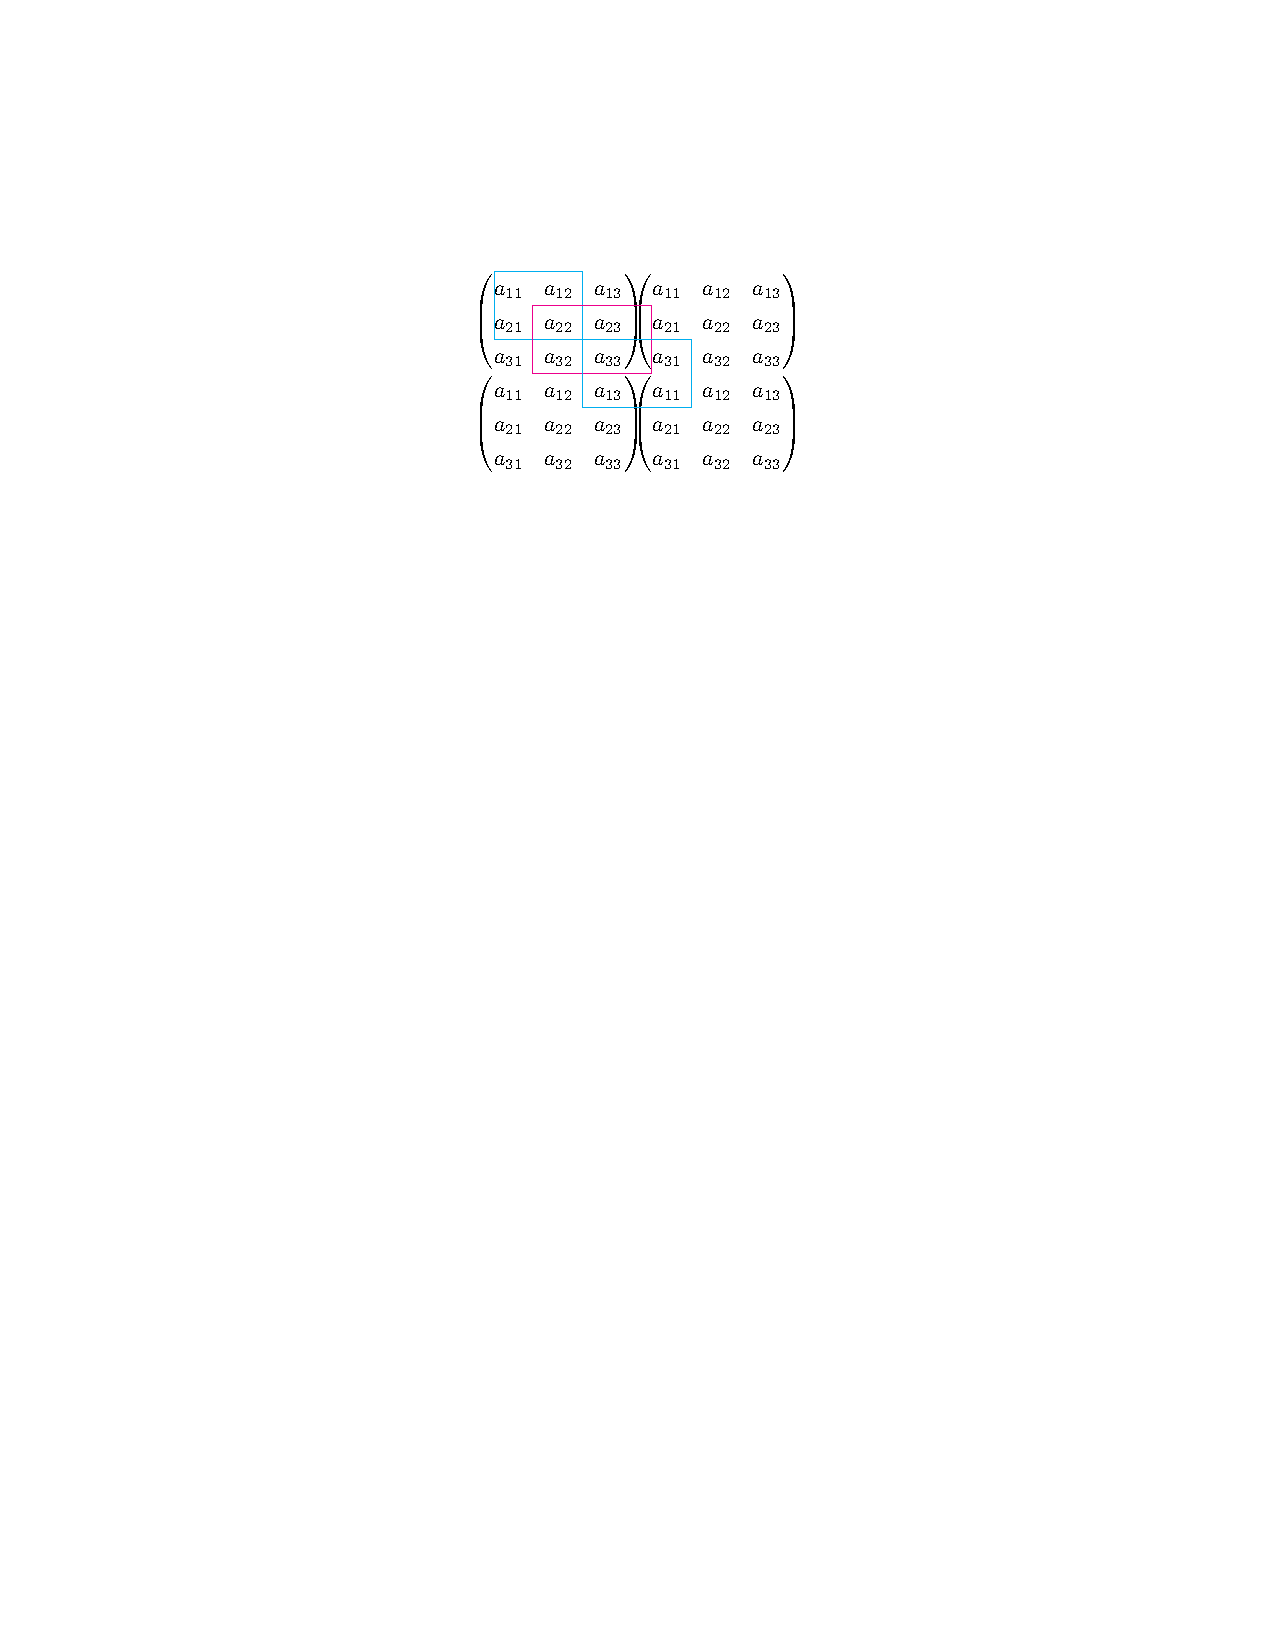
\includegraphics[scale=1]{figures/kjiezzshi.pdf}
    \caption{}
    \label{fig:kjiezzshi}
\end{figure}

\begin{theorem}[特征值的积与和]
    设 $n$ 阶方阵 $\vb*{A}$ 的特征值为 $\lambda_1,\lambda_2,\cdots,\lambda_n$, 则 $$\displaystyle\det\vb*{A}=\prod_{i=1}^{n}\lambda_i,~\tr\vb*{A}=\sum_{i=1}^{n}\lambda_i.$$
\end{theorem}

\begin{example}
    设 $\vb*{A}$ 是 3 阶矩阵, $\vb*{A}$ 的特征值为 $1,2,-1$, 如果 $\vb*{B}=\vb*{A}^2-2\vb*{A}+3\vb*{E}$, 求 $|\vb*{B}|$.
\end{example}
\begin{solution}
    易求得 $\vb*{B}$ 的特征值分别是 $2,3,6$, 那么 $\det\vb*{B}=2\times3\times6=36.$
\end{solution}

\begin{theorem}[逆矩阵的特征值]
    矩阵可逆当且仅当其特征值都不等于零, 若 $\lambda$ 是可逆矩阵 $\vb*{A}$ 的特征值, 则 $\dfrac{1}{\lambda}$ 是逆矩阵 $\vb*{A}^{-1}$ 的特征值.
\end{theorem}

\begin{theorem}[秩一矩阵的特征值]
    若 $n$ 阶方阵 $\vb*{A}$ 满足 $\rank\vb*{A}=1$, 那么矩阵 $\vb*{A}$ 的特征值为 $\tr\vb*{A}$ 及 $n-1$ 重 0 根.
\end{theorem}

\begin{example}
    已知 $\vb*{A}$ 是 3 阶矩阵, $\vb*{E}$ 是 3 阶单位矩阵, 如果 $\vb*{A},\vb*{A}-2\vb*{E},3\vb*{A}+2\vb*{E}$ 均不可逆, 求 $|\vb*{A}+\vb*{E}|.$
\end{example}
\begin{solution}
    易知矩阵 $\vb*{A}$ 的特征值分别为 $0,2,-\dfrac{2}{3}$, 那么 $\det(\vb*{A}+\vb*{E})=1\times3\times\dfrac{1}{3}=1.$
\end{solution}

\begin{theorem}[伴随矩阵的特征值 A]
    若 $\vb*{A}$ 为 $n$ 阶可逆矩阵, 且 $\lambda_i~ (i=1,2,\cdots,n)$ 是 $\vb*{A}$ 的全部特征值, 则 $\dfrac{|\vb*{A}|}{\lambda_i}$ 是 $\vb*{A}^*$ 的全部特征值; 
    若 $\vb*{A}$ 为 $n$ 阶不可逆矩阵, 则 $\vb*{A}^*$ 有 $n-1$ 个特征值为 0, 另一个特征值为 $\tr\vb*{A}^*.$
\end{theorem}

\begin{theorem}[伴随矩阵的特征值 B]
    \label{bsjzdtzzB}设 $n$ 阶方阵 $\vb*{A}$ 的特征值为 $\lambda_j~ (j=1,2,\cdots,n)$, 则 $\vb*{A}^*$ 的 $n$ 个特征值为 $\lambda_i^*$, 则
    $$\lambda_i^*=\prod_{\substack{1\leqslant j\leqslant n\\j\neq i}}\lambda_j~  (i=1,2,\cdots,n).$$
\end{theorem}

\begin{example}
    设 $ \vb*{A} $ 为 3 阶矩阵, 特征值为 $ \lambda_{1}=\lambda_{2}=1,\lambda_{3}=2 $, 
    对应的线性无关的特征向量为 $ \vb*{\alpha}_{1}, \vb*{\alpha}_{2}, \vb*{\alpha}_{3}$, 
    令 $ \vb*{P}=\left(\vb*{\alpha}_{1}-\vb*{\alpha}_{3}, \vb*{\alpha}_{2}+\vb*{\alpha}_{3}, \vb*{\alpha}_{3}\right)$, 则 $\vb*{P}^{-1} \vb*{A}^{*} \vb*{P}$ 等于
    \begin{tasks}(4)
        \task $\mqty(1&0&0\\0&3&0\\0&0&1)$
        \task $\mqty(-1&0&0\\0&3&0\\0&0&2)$
        \task $\mqty(2&0&1\\0&2&-1\\0&0&1)$
        \task $\mqty(2&0&0\\0&2&0\\1&-1&1)$
    \end{tasks}
\end{example}
\begin{solution}
    由 $\vb*{P}=(\vb*{\alpha}_{1}-\vb*{\alpha}_{3}, \vb*{\alpha}_{2}+\vb*{\alpha}_{3}, \vb*{\alpha}_{3})$, 得 $\vb*{P}=(\vb*{\alpha}_1,\vb*{\alpha}_2,\vb*{\alpha}_3)\vb*{E}_{31}(-1)\vb*{E}_{32}(1):=\vb*{B}\vb*{E}_{31}(-1)\vb*{E}_{32}(1)$, 那么
    \begin{flalign*}
        \vb*{P}^{-1}\vb*{A}^*\vb*{P}&=(\vb*{B}\vb*{E}_{31}(-1)\vb*{E}_{32}(1))^{-1}\vb*{A}^*\vb*{B}\vb*{E}_{31}(-1)\vb*{E}_{32}(1)=\vb*{E}_{32}(-1)\vb*{E}_{31}(1)\diag(2,2,1)\vb*{E}_{31}(-1)\vb*{E}_{32}(1)\\
        &=\vb*{E}_{32}(-1)\vb*{E}_{31}(1)\vb*{E}_{1}(2)\vb*{E}_{2}(2)\vb*{E}_{31}(-1)\vb*{E}_{32}(1)=\mqty(2&0&0\\0&2&0\\1&-1&1)
    \end{flalign*}
    因此选 D.
\end{solution}

\begin{example}
    已知矩阵 $\vb*{A}=\mqty(1&-1&a\\1&3&5\\0&0&2)$, 只有两个线性无关的特征向量, 求矩阵 $\vb*{A}$ 的特征值以及 $a$.
\end{example}
\begin{solution}
    由 $|\lambda\vb*{E}-\vb*{A}|=\mqty|\lambda-1&1&-a\\-1&\lambda-3&-5\\0&0&\lambda-2|=(\lambda-1)(\lambda-3)(\lambda-2)+(\lambda-2)=(\lambda-2)^3=0$, 于是特征值为 $\lambda_1=\lambda_2=\lambda_3=2$, 因为 $n-\rank(2\vb*{E}-\vb*{A})=2$, 于是 $\rank(2\vb*{E}-\vb*{A})=1$, 进而解得 $a=-5.$
\end{solution}

\begin{theorem}[特征值不等式]
    \label{tzzbds}若 $\vb*{A}$ 的特征值按从小到大排列, 即 $\lambda_1\leqslant \lambda_2\leqslant \cdots\leqslant \lambda_n$, 则 $$\lambda_1\vb*{x}^\top\vb*{x}\leqslant \vb*{x}^\top\vb*{Ax}\leqslant \lambda_n\vb*{x}^\top\vb*{x}.$$
\end{theorem}
\begin{proof}[{\songti \textbf{证}}]
    存在正交矩阵 $\vb*{Q}$, 令 $\vb*{x}=\vb*{Qy}$, 使得 $$f(x_1,x_2,\cdots,x_n)=\vb*{x}^\top\vb*{Ax}=\vb*{y}^\top\vb*{Q}^\top\vb*{AQy}=\lambda_1y_1^2+\lambda_2y_2^2+\cdots+\lambda_ny_n^2$$
    不妨设 $\lambda_1\leqslant \lambda_2\leqslant\cdots\leqslant\lambda_n$, 有 
    $$\lambda_1\sum_{k=1}^{n}y_k^2\leqslant \sum_{k=1}^{n}\lambda_ky_k^2\leqslant \lambda_n\sum_{k=1}^{n}y_k^2$$
    即 $$\lambda_1\vb*{x}^\top\vb*{x}\leqslant \vb*{x}^\top\vb*{Ax}\leqslant \lambda_n\vb*{x}^\top\vb*{x}.$$
\end{proof}

\begin{theorem}[行均和定理]
    \label{hangjunhedl}若矩阵 $\vb*{A}$ 的每行元素之和均为 $k$, 则 $\vb*{A}$ 有一特征值为 $k$, 所对应特征向量为 $(1,1,\cdots,1)^\top.$
\end{theorem}

\subsubsection{特征值在求解迭代方程中的应用}

\begin{example}
    给定 3 个数列 $\qty{x_n},\qty{y_n},\qty{z_n}$ 满足 $x_1=-2,y_1=1,z_1=-1$, 且当 $n\geqslant 1$ 有
    $$x_{n+1}=3x_n-6y_n-z_n,\quad y_{n+1}=-x_n+2y_n+z_n,\quad z_{n+1}=x_n+3y_n-z_n$$
    求极限 $\displaystyle\lim_{n\to\infty}\dfrac{x_n+y_n+z_n}{3^n+5^n}.$
\end{example}
\begin{solution}
    由 $\begin{cases}
            x_{n+1}=3x_n-6y_n-z_n \\
            y_{n+1}=-x_n+2y_n+z_n \\
            z_{n+1}=x_n+3y_n-z_n
        \end{cases}\Rightarrow \mqty(x_{n+1}\\y_{n+1}\\z_{n+1})=\mqty(3&-6&-1\\-1&2&1\\1&3&-1)\mqty(x_{n}\\y_n\\z_n):=\vb*{A}\mqty(x_{n}\\y_n\\z_n)$, 于是特征方程为
    $$\lambda^3-4\lambda^2-7\lambda+10=(\lambda-1)(\lambda-5)(\lambda+2)=0\Rightarrow \lambda_1=1,\lambda_2=5,\lambda_3=-2$$
    于是 $x_n+y_n+z_n=a\cdot 1^n+b\cdot 5^n+c\cdot (-2)^n$, 且
    $$\begin{cases}
            x_1+y_1+z_1=-2+1-1=-2=a+5b-2c   \\
            x_2+y_2+z_2=-11+3+3=-6=a+25b+4c \\
            x_3+y_3+z_3=-53+19-4=-38=a+125b-8c
        \end{cases}\Rightarrow \begin{cases}
            a=0             \\
            b=-\dfrac{2}{7} \\[6pt]
            c=\dfrac{2}{7}
        \end{cases}$$
    于是 $x_n+y_n+z_n=-\dfrac{2}{7}\cdot 5^n+\dfrac{2}{7}(-1)^n\cdot 2^n$, 那么 $\displaystyle\lim_{n\to\infty}\dfrac{-\dfrac{2}{7}\cdot 5^n+\dfrac{2}{7}(-1)^n\cdot 2^n}{3^n+5^n}=-\dfrac{2}{7}$.
\end{solution}

\subsection{矩阵的特征向量}

\begin{example}
    设矩阵 $\vb*{A}\mqty(3&2&2\\2&3&2\\2&2&3),~\vb*{P}=\mqty(0&1&0\\1&0&1\\0&0&1),~\vb*{B}=\vb*{P}^{-1}\vb*{A}^*\vb*{P}$, 求 $\vb*{B}+2\vb*{E}$ 的特征值与特征向量.
\end{example}
\begin{solution}
    设 $\vb*{A}$ 的特征值为 $\lambda$, 对应的特征向量为 $\vb*{\xi}$, 即 $\vb*{A\xi}=\lambda\vb*{\xi}$, 由于 $|\vb*{A}=7\neq0|$, 所以 $\lambda\neq0$, 于是有 
    $$\vb*{A}^*\vb*{\xi}=\dfrac{|\vb*{A}|}{\lambda}\vb*{\xi},~(\vb*{B}+2\vb*{E})\vb*{P}^{-1}\xi=\qty(\dfrac{|\vb*{A}|}{\lambda}+2)\vb*{P}^{-1}\xi$$
    即 $\dfrac{|\vb*{A}|}{\lambda}+2$ 是 $\vb*{B}+2\vb*{E}$ 的特征值, $\vb*{P}^{-1}\vb*{\xi}$ 为对应的特征向量, 
    易求得 $\vb*{A}$ 的特征值为 $\lambda_1=\lambda_2=1,\lambda_3=7$, 属于 $\lambda_{1,2}=1$ 的特征向量为 
    $$\vb*{\xi}_1=(-1,1,0)^\top,~\vb*{\xi}_2=(-1,0,1)^\top$$
    属于 $\lambda_3$ 的特征向量为 $\vb*{\xi}_3=(1,1,1)^\top$, 因此, $\vb*{B}+2\vb*{E}$ 的三个特征向量为 $9,9,3$, 属于特征值 9 的两个线性无关的特征向量为 
    $$\vb*{P}^{-1}\vb*{\xi}_1=(1,-1,0)^\top,~\vb*{P}^{-1}\vb*{\xi}_2=(-1,-1,1)^\top$$
    属于特征值 3 的特征向量为 $\vb*{P}^{-1}\vb*{\xi}_3=(0,1,1)^\top.$
\end{solution}

\begin{example}
    设 $\vb*{A}$ 是线性空间 $\vb*{P}^3$ 的线性变换, 已知
    $$\vb*{A}(1,0,0)=(5,6,-3),~\vb*{A}(0,1,0)=(-1,0,1),~\vb*{A}(0,0,1)=(1,2,1)$$
    \begin{enumerate}[label=(\arabic{*})]
        \item 求 $\vb*{A}$ 的全部特征值和特征向量;
        \item 问: 能否找到 $\vb*{P}^3$ 的一组基, 使 $\vb*{A}$ 在这组基下的矩阵为对角矩阵?说明理由.
    \end{enumerate}
\end{example}
\begin{solution}
    \begin{enumerate}[label=(\arabic{*})]
        \item $\vb*{A}$ 在基 $(1,0,0),~(0,1,0),~(0,0,1)$ 下的矩阵为
              $\begin{pmatrix}
                      5  & -1 & 1 \\
                      6  & 0  & 2 \\
                      -3 & 1  & 1
                  \end{pmatrix}$, 那么 $\vb*{A}$ 的特征多项式为
              $$f(\lambda)=|\lambda\vb*{E}-\vb*{A}|=\begin{vmatrix}
                      \lambda -5 & 1       & -1         \\
                      -6         & \lambda & -2         \\
                      -3         & -1      & \lambda -1
                  \end{vmatrix}\xlongequal[]{}(\lambda-2)^3$$
              所以 $\vb*{A}$ 的特征值为 2, 对 $\lambda=2$ 求特征向量, 解齐次方程组
              $$\left\{\begin{matrix}
                      -3x_1 & + & x_2  & - & x_3  & =0 \\
                      -6x_1 & + & 2x_2 & - & 2x_3 & =0 \\
                      3x_1  & - & x_2  & + & x_3  & =0
                  \end{matrix}\right.$$
              求得基础解系为: $(1,3,0),~(0,1,1)$, 所以 $\vb*{A}$ 的全部特征向量为 $k_1(1,3,0)+k_2(0,1,1)$, 其中 $k_1,~k_2$ 为数域 $\vb*{P}$
              中不全为零的任意数, 这些特征向量都属于特征值 2.
        \item 因为 $\vb*{A}$ 只有 2 个线性无关的特征向量, 而 $\vb*{P}^3$ 是 3 维线性空间, 所以找不到一组基, 使 $\vb*{A}$ 在这组基下的矩阵为对角矩阵.
    \end{enumerate}
\end{solution}

\begin{example}
    设 $\vb*{A}$ 是线性空间 $\vb*{P}^3$ 的线性变换, 
    已知 $$\vb*{A}(1,0,0)=(8,-6,3),~\vb*{A}(1,1,0)=(14,-10,6),~\vb*{A}(1,1,1)=(8,-4,5)$$
    求 $\vb*{A}$ 的全部特征值和特征向量, 并求 $\vb*{P}^3$ 的一组基使 $\vb*{A}$ 在这组基下的矩阵为对角矩阵.
\end{example}
\begin{solution}
    因为
    \begin{flalign*}
        \vb*{A}(1,0,0) & =(8,-6,3)=14(1,0,0)-9(1,1,0)+3(1,1,1)    \\
        \vb*{A}(1,1,0) & =(14,-10,6)=24(1,0,0)-16(1,1,0)+6(1,1,1) \\
        \vb*{A}(1,1,1) & =(8,-4,5)=12(1,0,0)-9(1,1,0)+5(1,1,1)
    \end{flalign*}
    所以 $\vb*{A}$ 在基 $(1,0,0),~(1,1,0),~(1,1,1)$ 下的矩阵为
    $\vb*{A}=\begin{pmatrix}
            14 & 24  & 12 \\
            -9 & -16 & -9 \\
            3  & 6   & 5
        \end{pmatrix}$, 
    $\vb*{A}$ 的特征多项式为
    $$f(\lambda)=|\lambda \vb*{E}-\vb*{A}|=\begin{vmatrix}
            \lambda -14 & -24         & -12        \\
            9           & \lambda +16 & 9          \\
            -3          & -6          & \lambda -5
        \end{vmatrix}\xlongequal[r_1-4r_3]{r_2+3r_3}\begin{vmatrix}
            \lambda -2 & 0          & -4\lambda +8 \\
            0          & \lambda -2 & 3\lambda -6  \\
            -3         & -6         & \lambda -5
        \end{vmatrix}=(\lambda-2)^2(\lambda+1)$$
    对 $\lambda=-1$ 解齐次方程组
    $$\left\{\begin{matrix}
            -15x_1 & - & 24x_2 & - & 12x_3 & =0 \\
            9x_1   & + & 15x_2 & + & 9x_3  & =0 \\
            -3x_1  & - & 6x_2  & - & 6x_3  & =0
        \end{matrix}\right.$$
    得基础解系: $(4,-3,1)$, 对应特征向量为 $4(1,0,0)-3(1,1,0)+(1,1,1)=(2,-2,1)$, 所以属于特征值 -1 的全部特征向量为 $k(2,-2,1)$, 
    其中 $k$ 为数域 $\vb*{P}$ 中任一非零数;\\
    对 $\lambda=2$ 解齐次方程组
    $$\left\{\begin{matrix}
            -12x_1 & - & 24x_2 & - & 12x_3 & =0 \\
            9x_1   & + & 18x_2 & + & 9x_3  & =0 \\
            -3x_1  & - & 6x_2  & - & 3x_3  & =0
        \end{matrix}\right.$$
        得基础解系 $(-1,0,1),~(0,-1,2)$, 对应于特征向量分别为
        $$-(1,0,0)+(1,1,1)=(0,1,1)\text{ 及 }-(1,1,0)+2(1,1,1)=(1,1,2)$$
        所以属于特征值 2 的全部特征向量为 $k_1(0,1,1)+k_2(1,1,2)$, 其中 $k_1,~k_2$ 为数域 $\vb*{P}$ 不全为 0 的任意性, 
        于是以 $$(2,-2,1),~(0,1,1),~(1,1,2)$$ 为基, 则 $\vb*{A}$ 在这组基下的矩阵为对角矩阵 $\mathrm{diag}(-1,2,2).$
\end{solution}

\begin{example}
    设 $\vb*{A}$ 是 3 阶矩阵, $\lambda_1,\lambda_2,\lambda_3$ 是 $\vb*{A}$ 的 3 个不同特征值, 对应的特征向量分别为 $\vb*{\alpha}_1,\vb*{\alpha}_2,\vb*{\alpha}_3$, 令 $\vb*{\beta}=\vb*{\alpha}_1+\vb*{\alpha}_2+\vb*{\alpha}_3$, 
    \begin{enumerate}[label=(\arabic{*})]
        \item 证明: $\vb*{\beta}=\vb*{\alpha}_1+\vb*{\alpha}_2+\vb*{\alpha}_3$ 不是 $\vb*{A}$ 的特征向量;
        \item 证明: $\vb*{\beta},\vb*{A\beta},\vb*{A^2\beta}$ 线性无关;
        \item 若 $\vb*{A}^3\vb*{\beta}=2\vb*{A\beta}$, 求 $\vb*{A}$ 的特征值;
        \item 在 (3) 的基础上证明: $\vb*{A\beta}$ 和 $\vb*{A}^2\vb*{\beta}$ 是方程组 $\qty(\vb*{A}^2-2\vb*{E})\vb*{x}=\vb*{0}$ 的基础解系.
    \end{enumerate}
\end{example}
\begin{solution}
    \begin{enumerate}[label=(\arabic{*})]
        \item 反证法: 假设 $\lambda$ 是 $\vb*{A}$ 的特征值, 且对应的特征向量为 $\vb*{\beta}$, 那么 $\vb*{A\beta}=\lambda\vb*{\beta}$, 即
              \begin{flalign*}
                  \vb*{A}(\vb*{\alpha}_1+\vb*{\alpha}_2+\vb*{\alpha}_3)                               & =\lambda(\vb*{\alpha}_1+\vb*{\alpha}_2+\vb*{\alpha}_3)             \\
                  \Rightarrow \vb*{A\alpha}_1+\vb*{A\alpha}_2+\vb*{A\alpha}_3                         & =\lambda\vb*{\alpha}_1+\lambda\vb*{\alpha}_2+\lambda\vb*{\alpha}_3 \\
                  \Rightarrow \lambda_1\vb*{\alpha}_1+\lambda_1\vb*{\alpha}_2+\lambda_1\vb*{\alpha}_3 & =\lambda\vb*{\alpha}_1+\lambda\vb*{\alpha}_2+\lambda\vb*{\alpha}_3 \\
              \end{flalign*}
              即 $\Rightarrow (\lambda_1-\lambda)\vb*{\alpha}_1+(\lambda_2-\lambda)\vb*{\alpha}_2+(\lambda_3-\lambda)\vb*{\alpha}_3=0$, 即 $\lambda_1=\lambda_2=\lambda_3$, 但这与题意矛盾, 故假设不成立, 
              即 $\vb*{\beta}=\vb*{\alpha}_1+\vb*{\alpha}_2+\vb*{\alpha}_3$ 不是 $\vb*{A}$ 的特征向量.
        \item 要证: $\vb*{\beta},\vb*{A\beta},\vb*{A^2\beta}$ 线性无关, 即证: $k_1\vb*{\beta}+k_2\vb*{A\beta}+k_3\vb*{A}^2\vb*{\beta}=\vb*{0}$, 其中 $k_1+k_2+k_3=0$, 为此, 则有
              $$k_1(\vb*{\alpha}_1+\vb*{\alpha}_2+\vb*{\alpha}_3)+k_2(\lambda_1\vb*{\alpha}_1+\lambda_2\vb*{\alpha}_2+\lambda_3\vb*{\alpha}_3)+k_3\qty(\lambda_1^2\vb*{\alpha}_1+\lambda_2^2\vb*{\alpha}_2+\lambda_3^2\vb*{\alpha}_3)=\vb*{0}$$
              为使等式成立, 则有 $$\begin{cases}
                  k_1+k_2\lambda_1+k_3\lambda_1^2=0 \\
                  k_1+k_2\lambda_2+k_3\lambda_2^2=0 \\
                  k_1+k_2\lambda_3+k_3\lambda_3^2=0
              \end{cases}\Rightarrow \mqty|1&\lambda_1&\lambda_1^2\\[6pt]1&\lambda_2&\lambda_2^2\\[6pt]1&\lambda_3&\lambda_3^2|$$
              该行列式为 Vandermonde 行列式, 则其值为 $(\lambda_2-\lambda_1)(\lambda_3-\lambda_1)(\lambda_3-\lambda_2)\neq0$, 故 $k_1+k_2+k_3=0$, 因此 $\vb*{\beta},\vb*{A\beta},\vb*{A^2\beta}$ 线性无关.
        \item 设矩阵 $\vb*{B}\sim\vb*{A}$, 且 $\exists\vb*{P}$ 使得 $\vb*{P}^{-1}\vb*{AP}=\vb*{B}$, 即 $\vb*{AP}=\vb*{PB}$, 不妨取 $\vb*{P}=\qty(\vb*{\beta},\vb*{A\beta},\vb*{A^2\beta})$, 因此
              $$\vb*{AP}=\qty(\vb*{A\beta},\vb*{A}^2\vb*{\beta},\vb*{A}^3\vb*{\beta})\xlongequal{\vb*{A}^3\vb*{\beta}=2\vb*{A\beta}}\qty(\vb*{A\beta},\vb*{A}^2\vb*{\beta},2\vb*{A\beta})=\qty(\vb*{\beta},\vb*{A\beta},\vb*{A^2\beta})\mqty(0&0&0\\1&0&2\\0&1&0)$$
              因此 $\vb*{B}=\mqty(0&0&0\\1&0&2\\0&1&0)$, 则特征值方程为 $|\lambda\vb*{E}-\vb*{B}|=\mqty|\lambda &0&0\\-1&\lambda&-2\\0&-1&\lambda|=\lambda\mqty|\lambda&-2\\-1&\lambda|=\lambda\qty(\lambda^2-2)=0$, 因此特征值为 $\lambda_1=0,\lambda_2=\sqrt{2},\lambda_3=-\sqrt{2}$.
        \item 为证: $\vb*{A\beta}$ 和 $\vb*{A}^2\vb*{\beta}$ 是方程组 $\qty(\vb*{A}^2-2\vb*{E})\vb*{x}=\vb*{0}$ 的基础解系, 需分别证:
              \begin{enumerate}[label=(\roman{*})]
                  \item $\vb*{A\beta}$ 和 $\vb*{A}^2\vb*{\beta}$ 是方程组 $\qty(\vb*{A}^2-2\vb*{E})\vb*{x}=\vb*{0}$ 的解;\\
                        当 $\vb*{x}=\vb*{A\beta}$ 时, 有 $\qty(\vb*{A}^2-2\vb*{E})\vb*{A\beta}=\vb*{A}^3\vb*{\beta}-2\vb*{A\beta}\xlongequal{\vb*{A}^3\vb*{\beta}=2\vb*{A\beta}}\vb*{0}$ 成立;\\
                        当 $\vb*{x}=\vb*{A}^2\vb*{\beta}$ 时, 有 $\qty(\vb*{A}^2-2\vb*{E})\vb*{A}^2\vb*{\beta}=\vb*{A}^4\vb*{\beta}-2\vb*{A}^2\vb*{\beta}=\vb*{A}\qty(\vb*{A}^3\vb*{\beta}-2\vb*{A\beta})\xlongequal{\vb*{A}^3\vb*{\beta}=2\vb*{A\beta}}\vb*{0}$ 成立;
                  \item $\vb*{A\beta}$ 和 $\vb*{A}^2\vb*{\beta}$ 线性无关;\\
                        由 (2) 可知 $\vb*{\beta},\vb*{A\beta},\vb*{A^2\beta}$ 线性无关 \textcolor{red}{(整体无关, 部分必无关; 部分相关, 整体必相关)}, 故 $\vb*{A\beta}$ 和 $\vb*{A}^2\vb*{\beta}$ 线性无关;
                  \item $S=n-\rank\qty(\vb*{A}^2-2\vb*{E})$, 其中 $S=2$.\\
                        因为 $\vb*{P}^{-1}\vb*{AP}=\vb*{\Lambda}_1$, 即 $\vb*{A}$ 能相似对角化, 故 $\vb*{P}^{-1}\qty(\vb*{A}^2-2\vb*{E})\vb*{P}$ 亦能相似对角化为矩阵 $\vb*{\Lambda}_2$, 又因为 $\qty(\vb*{A}^2-2\vb*{E})$ 的特征值为 $2,0,0$, 那么 $\rank\qty(\vb*{A}^2-2\vb*{E})=1$, 且 $n=3$, 故 $S=n-\rank\qty(\vb*{A}^2-2\vb*{E})$ 成立, 
              \end{enumerate}
              综上所述, $\vb*{A\beta}$ 和 $\vb*{A}^2\vb*{\beta}$ 是方程组 $\qty(\vb*{A}^2-2\vb*{E})\vb*{x}=\vb*{0}$ 的基础解系.
    \end{enumerate}
\end{solution}

%\section{矩阵相似与可对角化}

矩阵相似是指两个矩阵可以通过相似变换互相转换, 而矩阵可对角化是指将一个矩阵通过相似变换变为对角矩阵。两者之间的关系是:如果一个矩阵可对角化, 则它必定与某个对角矩阵相似;反之, 如果两个矩阵相似, 则它们可能都可对角化, 但不一定其中之一必定可对角化.

\subsection{矩阵的相似}

\begin{definition}[矩阵的相似]
    设 $\vb*{A}\text{, }\vb*{B}$ 是 $n$ 阶矩阵, 如果存在 $n$ 阶可逆矩阵 $\vb*{P}$, 使得 $$\vb*{P}^{-1}\vb*{AP}=\vb*{B}$$
    \index{矩阵相似}则称矩阵 $\vb*{A}$ 与 $\vb*{B}$ \textit{相似}, 记为 $\vb*{A}\sim\vb*{B}.$
\end{definition}

\begin{theorem}[相似的反身性]
    任意矩阵都与其自身相似, 即对于任意矩阵 $\vb*{A}$, 存在一个非奇异矩阵 $\vb*{E}$ (单位矩阵), 使得:
    $$\vb*{A}=\vb*{E}^{-1} \vb*{A I}=\vb*{A}.$$
\end{theorem}

\begin{theorem}[相似的对称性]
    如果矩阵 $\vb*{A}$ 和 $\vb*{B}$ 相似, 即存在一个非奇异矩阵 $\vb*{T}$ 使得:
    $$\vb*{B}=\vb*{T}^{-1} \vb*{A T}$$
    那么 $\vb*{A}$ 和 $\vb*{B}$ 也相似, 即存在一个非奇异矩阵 $\vb*{S}$ 使得:
    $$\vb*{A}=\vb*{S}^{-1} \vb*{B S}.$$
\end{theorem}

\begin{theorem}[相似的传递性]
    如果矩阵 $\vb*{A}$ 和 $\vb*{B}$ 相似, 且 $\vb*{B}$ 和 $\vb*{C}$ 相似, 那么 $\vb*{A}$ 和 $\vb*{C}$ 也相似, 即存在非奇异矩阵 $\vb*{T}$ 和 $\vb*{S}$ 使得:
    $$\vb*{B}=\vb*{T}^{-1} \vb*{A T}, \quad \vb*{C}=\vb*{S}^{-1} \vb*{B S}$$
    则存在一个非奇异矩阵 $\vb*{U}$ 使得:
    $$\vb*{A}=\vb*{U}^{-1} \vb*{C U}.$$
\end{theorem}

\begin{theorem}[矩阵相似的必要条件]
    若 $\vb*{A}$ 与 $\vb*{B}$ 是相似的, 则由相似矩阵的性质可得:
    \setcounter{magicrownumbers}{0}
    \begin{table}[H]
        \centering
        \caption{矩阵相似的必要条件}
        \begin{tabular}{l l l l}
            (\rownumber) $\det\vb*{A}=\det\vb*{B}.$      & (\rownumber) $\rank(\vb*{A})=\rank\vb*{B}.$ & (\rownumber) $\tr\vb*{A}=\tr\vb*{B}.$        & (\rownumber) $|\lambda\vb*{E}-\vb*{A}|=|\lambda\vb*{E}-\vb*{B}|.$ \\
            \midrule
            (\rownumber) $k\vb*{A}\sim k\vb*{B}$.        & (\rownumber) $\vb*{A}^{m}\sim\vb*{B}^{m}$.  & (\rownumber) $f(\vb*{A})\sim f(\vb*{B})$     & (\rownumber) $\vb*{AB}\sim \vb*{BA}.$                             \\
            \midrule
            (\rownumber) $\vb*{A}^{-1}\sim\vb*{B}^{-1}$. & (\rownumber) $\vb*{A}^*\sim\vb*{B}^*.$      & (\rownumber) $\vb*{A}^\top\sim\vb*{B}^\top$.
        \end{tabular}
    \end{table}
\end{theorem}

\begin{example}
    已知矩阵 $\vb*{A}\sim\vb*{B}$, 其中 $\vb*{B}=\mqty(0&0&1\\0&2&0\\3&0&0)$, 则 $|\vb*{A}+\vb*{E}|$.
\end{example}
\begin{solution}
    因为 $\vb*{A}\sim\vb*{B}$, 则 $|\vb*{A}+\vb*{E}|=|\vb*{B}+\vb*{E}|=-6.$
\end{solution}

\begin{example}
    已知矩阵 $\vb*{A}=\mqty(-2& -2& 1\\ 2& x& -2\\ 0& 0& -2)$ 与 $\vb*{B}=\mqty(2& 1& 0\\ 0& -1& 0\\ 0& 0& y)$ 相似, 求 $x$ 与 $y$.
\end{example}
\begin{solution}
    因为 $\vb*{A}$ 与 $\vb*{B}$ 相似, 故具有相同的迹和相同的行列式, 故 $\left\{\begin{matrix}
            x-4=1+y \\
            4x-8=-2y
        \end{matrix}\right.\Rightarrow x=3\text{, }y=-2.$
\end{solution}

\begin{example}
    设 $\vb*{A}=\mqty(1&0&0\\0&1&0\\2&2&-3)~,\vb*{B}=\mqty(1&2&0\\0&1&4\\0&0&-3)~,\vb*{C}=\mqty(2&1&-5\\0&1&0\\1&1&-4)~,\vb*{D}=\mqty(2&3&4\\0&1&-2\\5&1&-2)~,\vb*{\Lambda}=\diag(1,1,-3)$, 则在 $\vb*{A},\vb*{B},\vb*{C},\vb*{D}$ 中与 $\vb*{\Lambda}$ 相似的矩阵有 (\quad).
    \begin{tasks}(4)
        \task $\vb*{A},\vb*{C}$
        \task $\vb*{A},\vb*{D}$
        \task $\vb*{B},\vb*{C}$
        \task $\vb*{A},\vb*{D}$
    \end{tasks}
\end{example}
\begin{solution}
    矩阵相似有四个必要条件, 分别为: 秩相等, 迹相等, 行列式相等和特征多项式相等, 于是对于矩阵 $\vb*{D}$ 因为 $\tr\vb*{D}\neq\tr\vb*{\Lambda}$, 故排除选项 B、D, 又因为
    矩阵相似对角矩阵等价于它的每一个特征值的重数与其对应的线性无关的特征向量个数相等, 对于矩阵 $\vb*{B}$, 它的特征值显然是 $1,1,-3$ 与 $\vb*{\Lambda}$ 相同, 但是对于 $\lambda=1$ (二重),
    $$n-\rank(\lambda\vb*{E}-\vb*{B})=3-2=1\neq 2 (\text{特征值重数})$$
    因此矩阵 $\vb*{B}$ 关于特征值 1 仅一个线性无关的特征向量, 矩阵 $\vb*{B}$ 不能相似对角化为 $\vb*{\Lambda}$, 排除选项 C, 故选 A.
\end{solution}

\begin{example}[2013 数一]
    矩阵 $\vb*{A}=\mqty(1&a&1\\a&b&a\\1&a&1)$ 与 $\vb*{B}=\mqty(2&0&0\\0&b&0\\0&0&0)$ 相似的充要条件为 (\quad).
    \begin{tasks}(4)
        \task $a=0,b=2$
        \task $a=0,b$ 为任意常数
        \task $a=0,b=0$
        \task $a=2,b$ 为任意常数
    \end{tasks}
\end{example}
\begin{solution}
    因为矩阵 $\vb*{A}$ 是实对称矩阵, 矩阵 $\vb*{B}$ 是对角矩阵, 则 $\vb*{A}$ 与 $\vb*{B}$ 相似的充要条件是 $\vb*{A}$ 的特征值为 $2,b,0$,
    因为 $2$ 是 $\vb*{A}$ 的特征值, 那么 $$|2\vb*{E}-\vb*{A}|=0\Rightarrow a=0$$
    当 $a=0$ 时, $|\lambda\vb*{E}-\vb*{A}|=\lambda(\lambda-2)(\lambda-b)$
    那么 $\vb*{A}$ 的特征值为 $2,b,0$, 所以 $b$ 为任意常数即可, 选 B.
\end{solution}

\begin{example}[2009 兰州大学]
    已知矩阵 $\vb*{A}=\mqty(1&2&2\\2&a&2\\2&2&1)\text{, }\vb*{B}=\mqty(-1&0&0\\0&-1&0\\0&0&b)$, 问 $a\text{, }b$ 取何值时 $\vb*{A}$ 与 $\vb*{B}$ 相似? 并求可逆矩阵 $\vb*{P}$ 使得 $\vb*{P}^{-1}\vb*{AP}=\vb*{B}.$
\end{example}
\begin{solution}
    \textbf{法一: }由于 $\vb*{A}$ 与 $\vb*{B}$ 相似, 则它们的特征多项式相同, 所以 $|\lambda\vb*{E}-\vb*{A}|=|\lambda\vb*{E}-\vb*{B}|$, 即
    $$\mqty|\lambda-1 &-2 &-2\\-2 &\lambda-a &-2\\-2 &-2 &\lambda-1|=\mqty|\lambda+1 &0 &0\\0 &\lambda+1 &0\\0 &0 &\lambda-b|$$
    得 $(\lambda+1)\qty(\lambda^2-(3+a)\lambda+3a-8)=(\lambda+1)^2(\lambda-b)$, 比较两边的系数, 得 $a=1\text{, }b=5$, 那么
    $$f(\lambda)=\mqty|\lambda-1 &-2 &-2\\-2 &\lambda-1 &-2\\-2 &-2 &\lambda-1|\xlongequal[r_1-r_3]{r_2-r_3}(\lambda+1)^2\mqty|1 &0 &-1\\0 &1 &-1\\-2 &-2 &\lambda-1|=(\lambda+1)^2(\lambda-5)$$
    那么 $\vb*{A}$ 的特征值为 $-1$ (二重) 和 5, 则对应的特征向量依次为
    $$\vb*{\xi}_1=(-1,-1,0)^{\top}\text{, }\vb*{\xi}_2=(-1,0,-1)^{\top}\text{, }\vb*{\xi}_3=(1,1,1)^{\top}$$
    从而可得可逆矩阵 $\vb*{P}=(\vb*{\xi}_1,\vb*{\xi}_2,\vb*{\xi}_3)=\mqty(-1 &-1 &1\\1 &0 &1\\0 &1 &1)$, 容易验证有 $\vb*{P}^{-1}\vb*{AP}=\vb*{B}$, 故 $\vb*{P}$ 即使所求.\\
    \textbf{法二: }因为 $\vb*{A}$ 与 $\vb*{B}$ 相似, 所以具有相同的迹和相同的行列式, 即 $\tr\vb*{A}=\tr\vb*{B}\text{, }\det \vb*{A}=\det\vb*{B}$, 故
    $$2+a=-2+b\text{, }-3a+8=b$$ 解得 $a=1\text{, }b=5.$
\end{solution}

% \begin{example}
%     设 3 阶方阵 $\vb*{A}$ 和 $\vb*{B}$, 其中 $\vb*{A}=\mqty(1&2&3\\0&1&2\\0&0&1)\text{, }\vb*{B}=\mqty(1&0&0\\0&1&2\\0&0&1)$, 问: 矩阵 $\vb*{A}$ 与 $\vb*{B}$ 是否相似, 并说明理由.
% \end{example}
% \subsection{Hamilton-Cayley 定理}
% 
% \begin{example}
%     设 $\vb*{A}=\mqty(2&1&0\\0&2&1\\0&0&2)\text{, }f(x)=1+x+x^2+x^3+x^4+x^5+x^6+x^7$, 求 $f(\vb*{A}).$
% \end{example}
% \begin{solution}
%     易知 $\vb*{A}$ 的特征多项式 $g(\lambda)=(\lambda-2)^3$, 对 $f(\lambda)$ 利用带余除法, 得 $$f(\lambda)=g(\lambda)h(\lambda)+a\lambda^2+b\lambda+c$$
%     从而有 $$$$
% \end{solution}

\subsection{相似对角化}

\subsubsection{可相似对角化}

\begin{theorem}
    实对称矩阵一定能相似对角化.
\end{theorem}

\begin{theorem}
    若存在不相等的实数 $a,~b$, 使得 $(\vb*{A}-a\vb*{E})(\vb*{A}-b\vb*{E})=\vb*{O}$, 则矩阵 $\vb*{A}$ 一定能相似对角化.
\end{theorem}
\begin{proof}[{\songti \textbf{证}}]
    因为 $(\vb*{A}-a\vb*{E})(\vb*{A}-b\vb*{E})=\vb*{O}$, 所以 $$n=\rank((b-a)\vb*{E})=\rank[(\vb*{A}-a\vb*{E})-(\vb*{A}-b\vb*{E})]\leqslant \rank(\vb*{A}-a\vb*{E})+\rank(\vb*{A}-b\vb*{E})\leqslant n$$
    故 $\rank(\vb*{A}-a\vb*{E})+\rank(\vb*{A}-b\vb*{E})=n$, 因此 $\vb*{A}$ 的属于特征值 $a$ 的特征向量个数有 $n-\rank(\vb*{A}-a\vb*{E})$; 属于特征值 $b$ 的特征向量个数有 $n-\rank(\vb*{A}-b\vb*{E})$, 共有
    $$2n-\qty[\rank(\vb*{A}-a\vb*{E})+\rank(\vb*{A}-b\vb*{E})]=n$$
    又因为 $\vb*{A}$ 有 $n$ 个线性无关的特征向量等价于 $\vb*{A}$ 一定能相似对角化.
\end{proof}

\begin{example}
    设矩阵 $\vb*{A}=\begin{pmatrix} 0 & 2 & 0 \\ 1 & -1 & a+1 \\ 0 & 0 & 1 \\\end{pmatrix}, \vb*{B}=\begin{pmatrix} 1 & 0 & 0 \\ 0 & 1 & 0 \\ 0 & 0 & b \\\end{pmatrix}$, 且 $\vb*{A}$ 与 $\vb*{B}$ 相似, 求 $a+b.$
\end{example}
\begin{solution}
    因为 $\vb*{A}\sim \vb*{B}$, 所以 $\tr\vb*{A}=\tr\vb*{B}\Rightarrow b=-2$, 又 $\vb*{B}$ 为对角矩阵, 所以 $\vb*{A}$ 可相似对角化, 所以 $\rank(\vb*{E}-\vb*{A})=1$, 即
    $$
        \vb*{E}-\vb*{A}=\begin{pmatrix} 1 & -2 & 0 \\ -1 & 2 & -a-1 \\ 0 & 0 & 0 \\\end{pmatrix}\to \begin{pmatrix} 1 & -2 & 0 \\ 0 & 0 & -a-1 \\ 0 & 0 & 0 \\\end{pmatrix}
    $$
    因此 $a=-1$, 所以 $a+b=-3.$
\end{solution}

\begin{example}[2017 数一]
    已知矩阵 $\vb*{A}=\mqty(2&0&0\\0&2&1\\0&0&1)\text{, }\vb*{B}=\mqty(2&1&0\\0&2&0\\0&0&1)\text{, }\vb*{C}=\mqty(1&0&0\\0&2&0\\0&0&2)$, 则 (\quad).
    \begin{tasks}(2)
        \task $\vb*{A}$ 与 $\vb*{C}$ 相似, $\vb*{B}$ 与 $\vb*{C}$ 相似
        \task $\vb*{A}$ 与 $\vb*{C}$ 相似, $\vb*{B}$ 与 $\vb*{C}$ 不相似
        \task $\vb*{A}$ 与 $\vb*{C}$ 不相似, $\vb*{B}$ 与 $\vb*{C}$ 相似
        \task $\vb*{A}$ 与 $\vb*{C}$ 不相似, $\vb*{B}$ 与 $\vb*{C}$ 不相似
    \end{tasks}
\end{example}
\begin{solution}
    因为 $\vb*{A}$ 和 $\vb*{B}$ 都是上三角矩阵, 所以特征值都为 $2,2,1$, 那么 $$\rank(2\vb*{E}-\vb*{A})=\mqty(0&0&0\\0&0&-1\\0&0&1)=1=3-2$$
    于是 $\vb*{A}$ 与 $\vb*{C}$ 相似; 同理 $$\rank(2\vb*{E}-\vb*{B})=\mqty(0&-1&0\\0&0&0\\0&0&1)=2\neq3-2$$
    所以 $\vb*{B}$ 与 $\vb*{C}$ 不相似, 选 B.
\end{solution}

\begin{example}
    设矩阵 $\vb*{A}=\mqty(0&1&0&0\\1&0&0&0\\0&0&y&1\\0&0&1&2)$
    \begin{enumerate}[label=(\arabic{*})]
        \item 已知 $\vb*{A}$ 的一个特征值为 3, 求 $y$;
        \item 求矩阵 $\vb*{P}$, 使得 $\vb*{AP}^{\top}(\vb*{AP})$ 为对角矩阵.
    \end{enumerate}
\end{example}
\begin{solution}
    \begin{enumerate}[label=(\arabic{*})]
        \item 因为 $$|\lambda\vb*{E}-\vb*{A}|=\mqty|\lambda&-1&0&0\\-1&\lambda&0&0\\0&0&\lambda-y&-1\\0&0&-1&\lambda-2|=\mqty|\lambda&-1\\-1&\lambda|\cdot\mqty|\lambda-y&-1\\-1&\lambda-2|=\qty(\lambda^2-1)[(\lambda-y)(\lambda-2)-1]=0$$
              将 $\lambda=3$ 代入得, $y=2$.
        \item 由 (1) 可知 $\vb*{A}=\mqty(0&1&0&0\\1&0&0&0\\0&0&2&1\\0&0&1&2)$, 那么 $\vb*{A}^\top=\vb*{A}$, 得 $(\vb*{AP})^\top(\vb*{AP})=\vb*{P}^\top\vb*{A}^2\vb*{P}$,
              而 $\vb*{A}^2=\mqty(1&0&0&0\\0&1&0&0\\0&0&5&4\\0&0&4&5)$, 由 $|\lambda\vb*{E}-\vb*{A}^2|=0$ 解得 $\lambda_1=1$ (三重), $\lambda_2=9$, 对应 $\lambda_1=1$ 的特征向量为
              $$\vb*{\alpha}_1=(1,0,0,0)^\top\text{, }\vb*{\alpha}_2=(0,1,0,0)^\top\text{, }\vb*{\alpha}_3=(0,0,-1,1)^\top$$
              标准正交化得 $$\vb*{\beta}_1=(1,0,0,0)^\top\text{, }\vb*{\beta}_2=(0,1,0,0)^\top\text{, }\vb*{\beta}_3=\dfrac{1}{\sqrt{2}}(0,0,-1,1)^\top$$
              对应于 $\lambda_2=9$ 的特征向量为 $\vb*{\alpha}_4=(0,0,1,1)^\top$, 经过单位化后, $\vb*{\beta}_4=\dfrac{1}{\sqrt{2}}(0,0,1,1)^\top$, 于是
              $$\vb*{P}=(\vb*{\beta}_1,\vb*{\beta}_2,\vb*{\beta}_3,\vb*{\beta}_4)=\mqty(1&0&0&0\\0&1&0&0\\0&0&-\dfrac{1}{\sqrt{2}}&\dfrac{1}{\sqrt{2}}\\[6pt]0&0&\dfrac{1}{\sqrt{2}}&\dfrac{1}{\sqrt{2}})\text{, }(\vb*{AP})^\top(\vb*{AP})=\mqty(\dmat{1,1,1,9}).$$
    \end{enumerate}
\end{solution}

\begin{example}
    设矩阵 $\vb*{A}=\mqty(1& -1& 1\\ x& 4& y\\ -3& -3& 5)$ 有 $3$ 个线性无关的特征向量, 且 $\lambda=2$ 是 $\vb*{A}$ 的二重特征值.
    \begin{enumerate}[label=(\arabic{*})]
        \item 求 $x\text{, }y$ 的值;
        \item 求可逆矩阵 $\vb*{P}$, 使得 $\vb*{P}^{-1}\vb*{AP}$ 为对角矩阵.
    \end{enumerate}
\end{example}
\begin{solution}
    \begin{enumerate}[label=(\arabic{*})]
        \item 根据题设, $\vb*{A}$ 有 3 个线性无关的特征向量, 所以 $\vb*{A}$ 可对角化, $\vb*{A}$ 的任一特征值的几何重数与代数重数相等, 对于特征值 $\lambda=2$ (二重), $\vb*{A}$
              有两个线性无关的特征向量, 由此可知 $\rank(2\vb*{E}-\vb*{A})=1$, 利用初等行变化, 得
              $$2\vb*{E}-\vb*{A}=\mqty(\dmat{2,2,2})-\mqty(1 &-1 &1\\ x &4 &y\\ -3 &-3 &5)=\mqty(1 &1 &-1\\ -x &-2 &-y\\ 3 &3 &-3)\xrightarrow[r_3-3r_1]{r_2+r_1\cdot x}\mqty(1 &1 &-1\\ 0 &x-2 &-y-x\\ 0 &0 &0)$$
              因此, 有 $x=2\text{, }y=-2.$
        \item 由 (1) 可知, $\vb*{A}=\mqty(1 &-1 &1\\ 2 &4 &-2\\ -3 &-3 &5)$, 那么矩阵 $\vb*{A}$ 的特征多项式为
              $$f(\lambda)=|\lambda\vb*{E}-\vb*{A}|=\mqty|\lambda-1 &1 &-1\\ -2 &\lambda-4 &2\\ 3 &3 &\lambda-5|\xlongequal[r_3-3r_1]{r_2+2r_1}\mqty|\lambda-1 &1 &-1\\ 2\lambda-4 &\lambda-2 &0\\ 6-3\lambda &0 &\lambda-2|=(\lambda-2)(\lambda-6)$$
              解得 $\lambda_1=\lambda_2=2\text{, }\lambda_3=6$, 对于特征值 $\lambda_{1,2}=2$, 解齐次方程组 $(2\vb*{E}-\vb*{A})\vb*{x}=\vb*{0}$, 对应的特征向量为
              $\vb*{\alpha}_1=(1,-1,0)^\top\text{, }\vb*{\alpha}_2=(1,0,1)^\top$,
              对于特征值 $\lambda_{3}=6$, 解齐次方程组 $(6\vb*{E}-\vb*{A})\vb*{x}=\vb*{0}$, 对应的特征向量为
              $\vb*{\alpha}_3=(1,-2,3)^\top$,
              令 $\vb*{P}=(\vb*{\alpha}_1,\vb*{\alpha}_2,\vb*{\alpha}_3)=\mqty(1 &1 &1\\ -1 &0 &-2\\ 0 &1 &3)$, 则 $\vb*{P}^{-1}\vb*{AP}=\mqty(\dmat{2,2,6})$ 为对角矩阵.
    \end{enumerate}
\end{solution}

\subsubsection{不可相似对角化}

假如三阶矩阵 $\vb*{A}$ 的特征值为 $a,b,b$, 那么有 $$\vb*{A}\text{ 可相似对角化}\Leftrightarrow\rank(b\vb*{E}-\vb*{A})=\text{阶数}-b\text{ 的重数}$$
即只需要判断 $\rank(b\vb*{E}-\vb*{A})\xlongequal{?}\text{阶数}-b\text{ 的重数}.$

\begin{example}
    设 3 阶矩阵 $\vb*{A}=\begin{pmatrix} a & 2 & 2 \\ 0 & 1 & 2 \\ 0 & 0 & -1 \\\end{pmatrix}$ 不能相似对角化, 求 $a$.
\end{example}
\begin{solution}
    $|\lambda\vb*{E}-\vb*{A}|=(\lambda-a)(\lambda-1)(\lambda+1)=0\Rightarrow \lambda_1=a, \lambda_2=1, \lambda_3=-1$, 当 $a=1$ 时 $$
        \rank(\vb*{E}-\vb*{A})=\rank \begin{pmatrix} 0 & -2 & -2 \\ 0 & 0 & -2 \\ 0 & 0 & -2 \\\end{pmatrix}=2\neq 3-2=1
    $$
    故当 $a=1$ 时, $\vb*{A}$ 不能相似对角化 (可验证 $a=-1$ 时, $\vb*{A}$ 能相似对角化).
\end{solution}

% \begin{figure}[H]
%     \centering
%     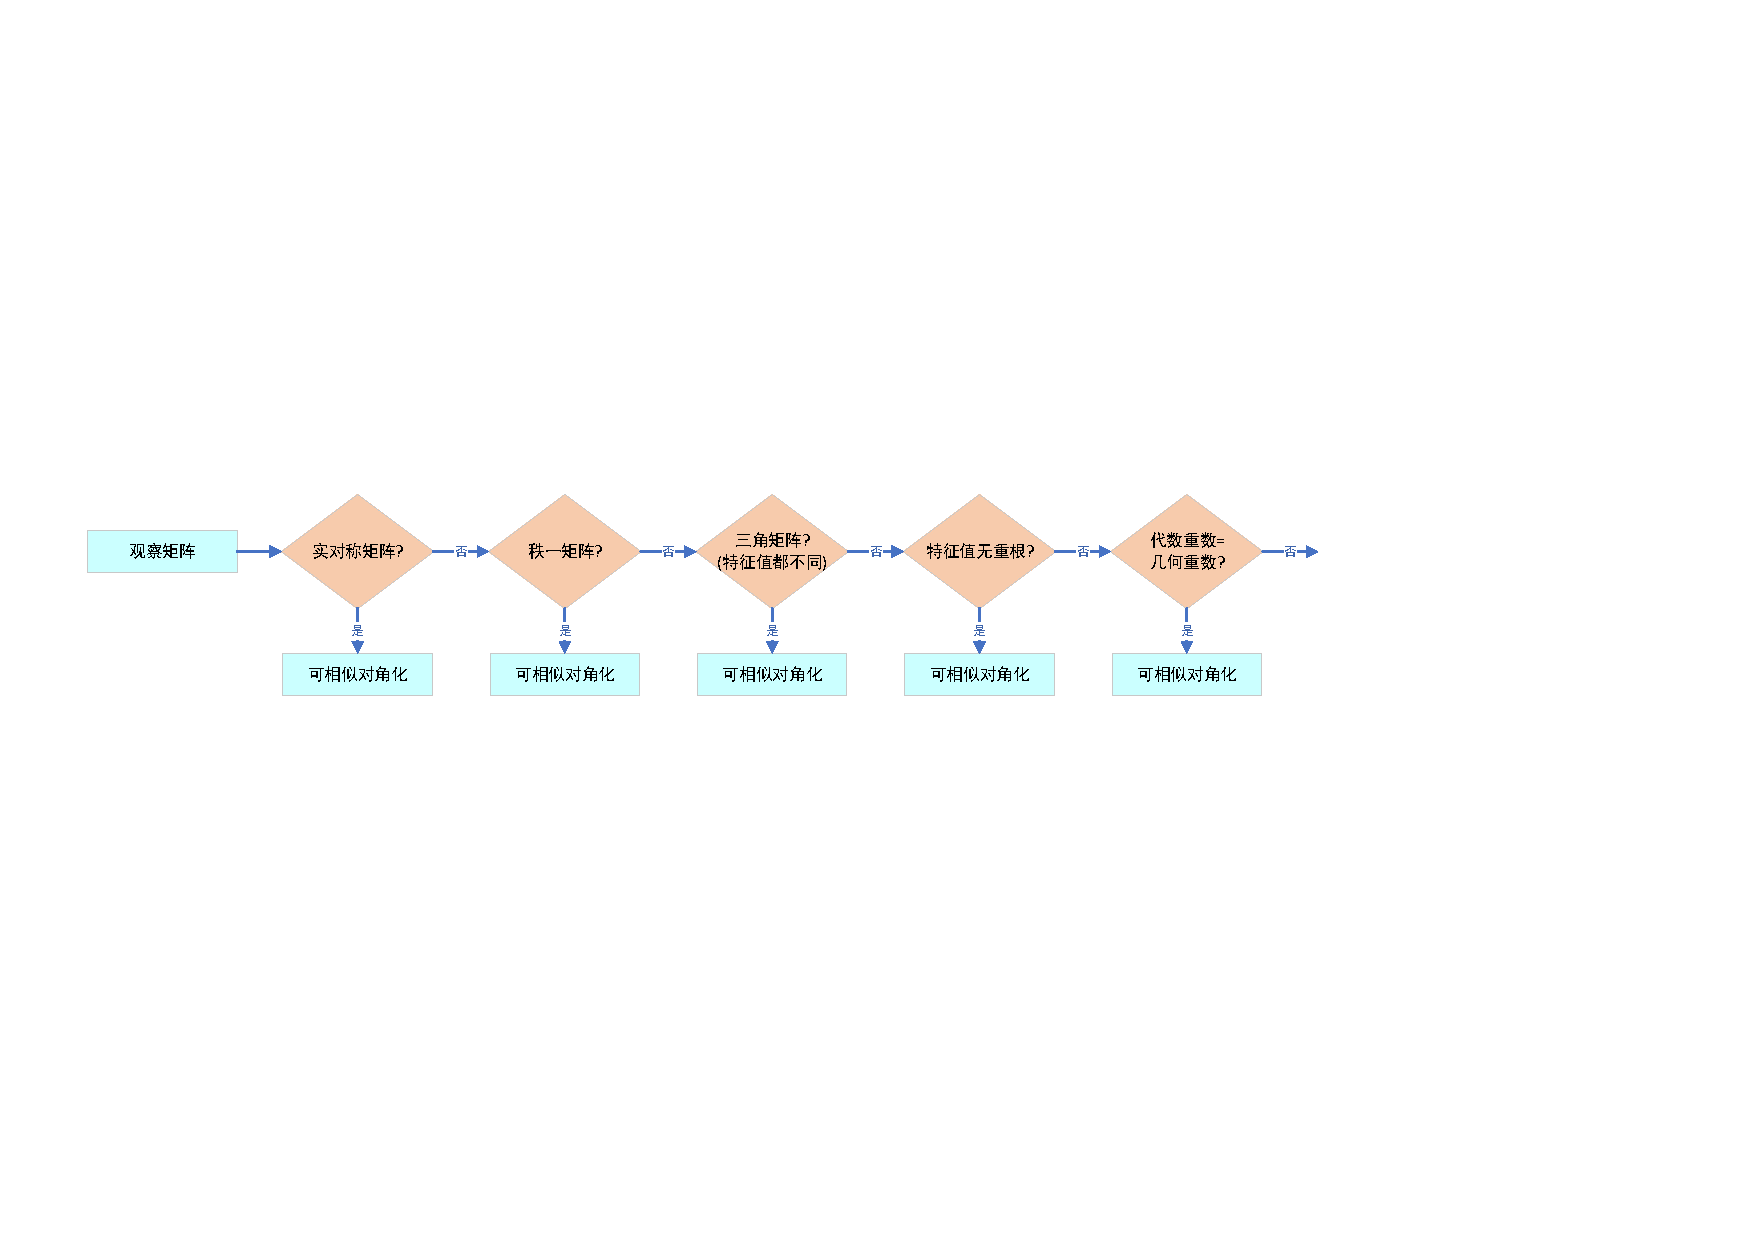
\includegraphics[scale=0.6]{figures/sdcjz.pdf}
%     \caption{}
%     \label{figure:sdcjz}
% \end{figure}

\begin{example}[2004 数一]
    设矩阵 $\vb*{A}=\mqty(1&2&-3\\-1&4&-3\\1&a&5)$ 的特征方程有一个二重根, 求 $a$ 的值, 并讨论 $\vb*{A}$ 是否可相似对角化.
\end{example}
\begin{solution}
    $|\lambda\vb*{E}-\vb*{A}|=\mqty|\lambda-1&-2&3\\1&\lambda-4&3\\-1&-a&\lambda-5|\xlongequal[r_2+r_3]{r_1-r_2}\mqty|\lambda-2&2-\lambda&0\\0&\lambda-4-a&\lambda-2\\-1&-a&\lambda-5|=(\lambda-2)\qty[(\lambda-5)(\lambda-4-a)+(\lambda-2)(1+a)]$,
    当 $\lambda=2$ 是方程的二重根时, 则有 $(2-5)(2-4-a)=0\Rightarrow a=-2$, 于是 $\vb*{A}=\mqty(1&2&-3\\-1&4&-3\\1&-2&5)$, 此时,
    $$\rank(2\vb*{E}-\vb*{A})=\rank\mqty(1&-2&3\\1&-2&3\\-1&2&-3)=\rank\mqty(0&0&0\\0&0&0\\-1&2&-3)=1=3-2$$
    因此可以相似对角化; 当 $2$ 不是方程的二重根时, $[(\lambda-5)(\lambda-4-a)+(\lambda-2)(1+a)]$ 为完全平方数, 解得 $a=-\dfrac{2}{3}$, 此时 $4$ 是该方程的二重根,
    于是 $\vb*{A}=\mqty(1&2&-3\\-1&4&-3\\1&-\dfrac{2}{3}&5)$, $\rank(4\vb*{E}-\vb*{A})\neq 1$, 于是 $a=-\dfrac{2}{3}$ 时, $\vb*{A}$ 不能相似对角化.
\end{solution}

\section{矩阵的特征值与特征向量}

\subsection{矩阵的特征值}

\begin{theorem}[特征多项式展开定理]
    设 $\vb*{A}$ 是 $n$ 阶矩阵,则 $\vb*{A}$ 的特征多项式为 
    $$f(\lambda)=|\lambda\vb*{E}-\vb*{A}|=\lambda^n-a_1\lambda^{n-1}+\cdots+(-1)^ka_k\lambda^{n-k}+\cdots+(-1)^na_n$$
    其中 $a_k$ 是 $\vb*{A}$ 的所有 $k$ 阶主子式之和,即 
    $$a_k=\sum_{1\leqslant j_1<\cdots<j_k\leqslant n}\mqty|a_{j_1j_1}&\cdots&a_{j_1j_k}\\\vdots&&\vdots\\a_{j_kj_1}&\cdots&a_{j_kj_k}|$$
    特别地 $a_1=\tr\vb*{A},~a_n=\det\vb*{A}.$
    对于常见的 3 阶矩阵有 $$f(\lambda)=\lambda^3-\tr\vb*{A}\cdot\lambda^2+\qty(\mqty|a_{11}&a_{12}\\a_{21}&a_{22}|+\mqty|a_{11}&a_{13}\\a_{31}&a_{32}|+\mqty|a_{22}&a_{23}\\a_{32}&a_{33}|)\lambda-\det\vb*{A}.$$
\end{theorem}

图 \ref{fig:kjiezzshi} 是 $a_2$ 的形象化表达.
\begin{figure}[H]
    \centering
    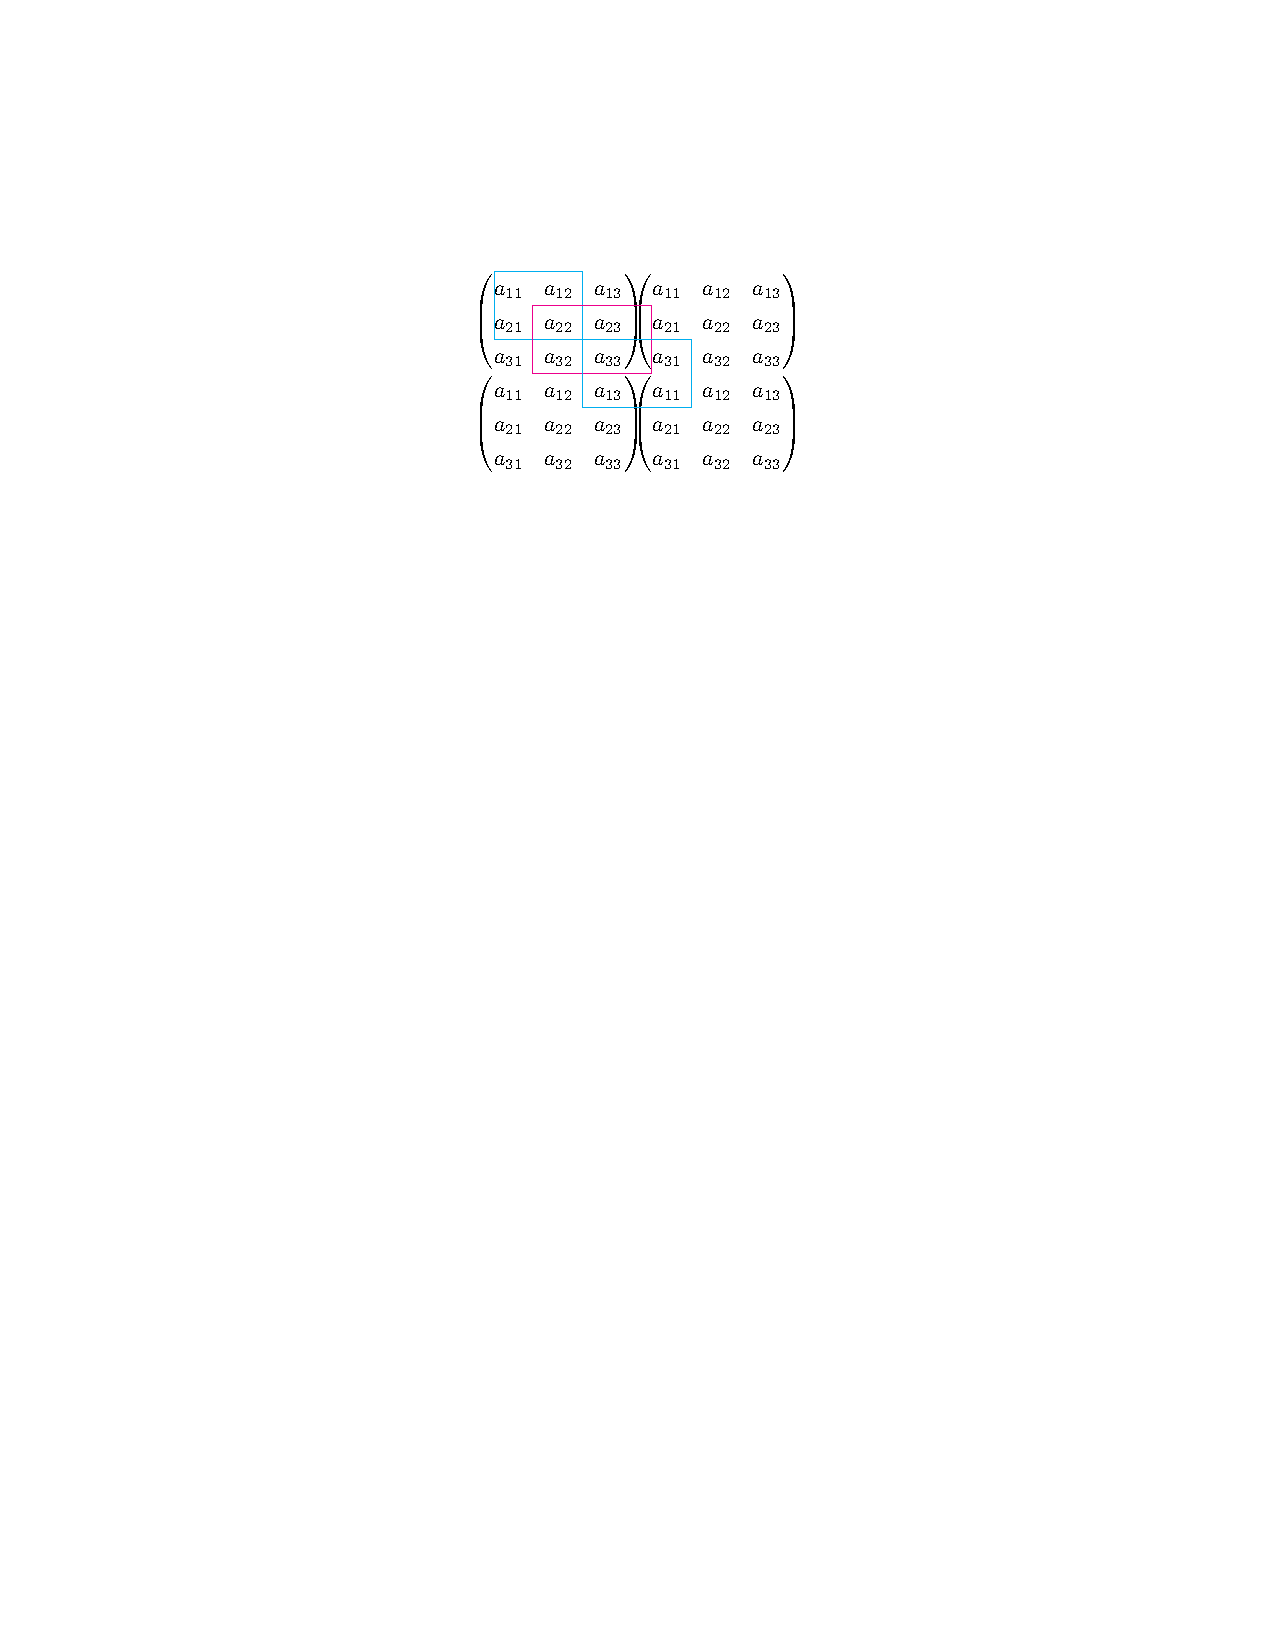
\includegraphics[scale=1]{figures/kjiezzshi.pdf}
    \caption{}
    \label{fig:kjiezzshi}
\end{figure}

\begin{theorem}[特征值的积与和]
    设 $n$ 阶方阵 $\vb*{A}$ 的特征值为 $\lambda_1,\lambda_2,\cdots,\lambda_n$,则 $$\displaystyle\det\vb*{A}=\prod_{i=1}^{n}\lambda_i,~\tr\vb*{A}=\sum_{i=1}^{n}\lambda_i.$$
\end{theorem}

\begin{example}
    设 $\vb*{A}$ 是 3 阶矩阵,$\vb*{A}$ 的特征值为 $1,2,-1$,如果 $\vb*{B}=\vb*{A}^2-2\vb*{A}+3\vb*{E}$,求 $|\vb*{B}|$.
\end{example}
\begin{solution}
    易求得 $\vb*{B}$ 的特征值分别是 $2,3,6$,那么 $\det\vb*{B}=2\times3\times6=36.$
\end{solution}

\begin{theorem}[逆矩阵的特征值]
    矩阵可逆当且仅当其特征值都不等于零,若 $\lambda$ 是可逆矩阵 $\vb*{A}$ 的特征值,则 $\dfrac{1}{\lambda}$ 是逆矩阵 $\vb*{A}^{-1}$ 的特征值.
\end{theorem}

\begin{theorem}[秩一矩阵的特征值]
    若 $n$ 阶方阵 $\vb*{A}$ 满足 $\rank\vb*{A}=1$,那么矩阵 $\vb*{A}$ 的特征值为 $\tr\vb*{A}$ 及 $n-1$ 重 0 根.
\end{theorem}

\begin{example}
    已知 $\vb*{A}$ 是 3 阶矩阵,$\vb*{E}$ 是 3 阶单位矩阵,如果 $\vb*{A},\vb*{A}-2\vb*{E},3\vb*{A}+2\vb*{E}$ 均不可逆,求 $|\vb*{A}+\vb*{E}|.$
\end{example}
\begin{solution}
    易知矩阵 $\vb*{A}$ 的特征值分别为 $0,2,-\dfrac{2}{3}$,那么 $\det(\vb*{A}+\vb*{E})=1\times3\times\dfrac{1}{3}=1.$
\end{solution}

\begin{theorem}[伴随矩阵的特征值 A]
    若 $\vb*{A}$ 为 $n$ 阶可逆矩阵,且 $\lambda_i~ (i=1,2,\cdots,n)$ 是 $\vb*{A}$ 的全部特征值,则 $\dfrac{|\vb*{A}|}{\lambda_i}$ 是 $\vb*{A}^*$ 的全部特征值; 
    若 $\vb*{A}$ 为 $n$ 阶不可逆矩阵,则 $\vb*{A}^*$ 有 $n-1$ 个特征值为 0,另一个特征值为 $\tr\vb*{A}^*.$
\end{theorem}

\begin{theorem}[伴随矩阵的特征值 B]
    \label{bsjzdtzzB}设 $n$ 阶方阵 $\vb*{A}$ 的特征值为 $\lambda_j~ (j=1,2,\cdots,n)$,则 $\vb*{A}^*$ 的 $n$ 个特征值为 $\lambda_i^*$,则
    $$\lambda_i^*=\prod_{\substack{1\leqslant j\leqslant n\\j\neq i}}\lambda_j~  (i=1,2,\cdots,n).$$
\end{theorem}

\begin{example}
    设 $ \vb*{A} $ 为 3 阶矩阵,特征值为 $ \lambda_{1}=\lambda_{2}=1,\lambda_{3}=2 $,
    对应的线性无关的特征向量为 $ \vb*{\alpha}_{1}, \vb*{\alpha}_{2}, \vb*{\alpha}_{3}$,
    令 $ \vb*{P}=\left(\vb*{\alpha}_{1}-\vb*{\alpha}_{3}, \vb*{\alpha}_{2}+\vb*{\alpha}_{3}, \vb*{\alpha}_{3}\right)$,则 $\vb*{P}^{-1} \vb*{A}^{*} \vb*{P}$ 等于
    \begin{tasks}(4)
        \task $\mqty(1&0&0\\0&3&0\\0&0&1)$
        \task $\mqty(-1&0&0\\0&3&0\\0&0&2)$
        \task $\mqty(2&0&1\\0&2&-1\\0&0&1)$
        \task $\mqty(2&0&0\\0&2&0\\1&-1&1)$
    \end{tasks}
\end{example}
\begin{solution}
    由 $\vb*{P}=(\vb*{\alpha}_{1}-\vb*{\alpha}_{3}, \vb*{\alpha}_{2}+\vb*{\alpha}_{3}, \vb*{\alpha}_{3})$,得 $\vb*{P}=(\vb*{\alpha}_1,\vb*{\alpha}_2,\vb*{\alpha}_3)\vb*{E}_{31}(-1)\vb*{E}_{32}(1):=\vb*{B}\vb*{E}_{31}(-1)\vb*{E}_{32}(1)$,那么
    \begin{flalign*}
        \vb*{P}^{-1}\vb*{A}^*\vb*{P}&=(\vb*{B}\vb*{E}_{31}(-1)\vb*{E}_{32}(1))^{-1}\vb*{A}^*\vb*{B}\vb*{E}_{31}(-1)\vb*{E}_{32}(1)=\vb*{E}_{32}(-1)\vb*{E}_{31}(1)\diag(2,2,1)\vb*{E}_{31}(-1)\vb*{E}_{32}(1)\\
        &=\vb*{E}_{32}(-1)\vb*{E}_{31}(1)\vb*{E}_{1}(2)\vb*{E}_{2}(2)\vb*{E}_{31}(-1)\vb*{E}_{32}(1)=\mqty(2&0&0\\0&2&0\\1&-1&1)
    \end{flalign*}
    因此选 D.
\end{solution}

\begin{example}
    已知矩阵 $\vb*{A}=\mqty(1&-1&a\\1&3&5\\0&0&2)$,只有两个线性无关的特征向量,求矩阵 $\vb*{A}$ 的特征值以及 $a$.
\end{example}
\begin{solution}
    由 $|\lambda\vb*{E}-\vb*{A}|=\mqty|\lambda-1&1&-a\\-1&\lambda-3&-5\\0&0&\lambda-2|=(\lambda-1)(\lambda-3)(\lambda-2)+(\lambda-2)=(\lambda-2)^3=0$,于是特征值为 $\lambda_1=\lambda_2=\lambda_3=2$,因为 $n-\rank(2\vb*{E}-\vb*{A})=2$,于是 $\rank(2\vb*{E}-\vb*{A})=1$,进而解得 $a=-5.$
\end{solution}

\begin{theorem}[特征值不等式]
    \label{tzzbds}若 $\vb*{A}$ 的特征值按从小到大排列,即 $\lambda_1\leqslant \lambda_2\leqslant \cdots\leqslant \lambda_n$,则 $$\lambda_1\vb*{x}^\top\vb*{x}\leqslant \vb*{x}^\top\vb*{Ax}\leqslant \lambda_n\vb*{x}^\top\vb*{x}.$$
\end{theorem}
\begin{proof}[{\songti \textbf{证}}]
    存在正交矩阵 $\vb*{Q}$,令 $\vb*{x}=\vb*{Qy}$,使得 $$f(x_1,x_2,\cdots,x_n)=\vb*{x}^\top\vb*{Ax}=\vb*{y}^\top\vb*{Q}^\top\vb*{AQy}=\lambda_1y_1^2+\lambda_2y_2^2+\cdots+\lambda_ny_n^2$$
    不妨设 $\lambda_1\leqslant \lambda_2\leqslant\cdots\leqslant\lambda_n$,有 
    $$\lambda_1\sum_{k=1}^{n}y_k^2\leqslant \sum_{k=1}^{n}\lambda_ky_k^2\leqslant \lambda_n\sum_{k=1}^{n}y_k^2$$
    即 $$\lambda_1\vb*{x}^\top\vb*{x}\leqslant \vb*{x}^\top\vb*{Ax}\leqslant \lambda_n\vb*{x}^\top\vb*{x}.$$
\end{proof}

\begin{theorem}[行均和定理]
    \label{hangjunhedl}若矩阵 $\vb*{A}$ 的每行元素之和均为 $k$,则 $\vb*{A}$ 有一特征值为 $k$,所对应特征向量为 $(1,1,\cdots,1)^\top.$
\end{theorem}

\subsubsection{特征值在求解迭代方程中的应用}

\begin{example}
    给定 3 个数列 $\qty{x_n},\qty{y_n},\qty{z_n}$ 满足 $x_1=-2,y_1=1,z_1=-1$,且当 $n\geqslant 1$ 有
    $$x_{n+1}=3x_n-6y_n-z_n,\quad y_{n+1}=-x_n+2y_n+z_n,\quad z_{n+1}=x_n+3y_n-z_n$$
    求极限 $\displaystyle\lim_{n\to\infty}\dfrac{x_n+y_n+z_n}{3^n+5^n}.$
\end{example}
\begin{solution}
    由 $\begin{cases}
            x_{n+1}=3x_n-6y_n-z_n \\
            y_{n+1}=-x_n+2y_n+z_n \\
            z_{n+1}=x_n+3y_n-z_n
        \end{cases}\Rightarrow \mqty(x_{n+1}\\y_{n+1}\\z_{n+1})=\mqty(3&-6&-1\\-1&2&1\\1&3&-1)\mqty(x_{n}\\y_n\\z_n):=\vb*{A}\mqty(x_{n}\\y_n\\z_n)$,于是特征方程为
    $$\lambda^3-4\lambda^2-7\lambda+10=(\lambda-1)(\lambda-5)(\lambda+2)=0\Rightarrow \lambda_1=1,\lambda_2=5,\lambda_3=-2$$
    于是 $x_n+y_n+z_n=a\cdot 1^n+b\cdot 5^n+c\cdot (-2)^n$,且
    $$\begin{cases}
            x_1+y_1+z_1=-2+1-1=-2=a+5b-2c   \\
            x_2+y_2+z_2=-11+3+3=-6=a+25b+4c \\
            x_3+y_3+z_3=-53+19-4=-38=a+125b-8c
        \end{cases}\Rightarrow \begin{cases}
            a=0             \\
            b=-\dfrac{2}{7} \\[6pt]
            c=\dfrac{2}{7}
        \end{cases}$$
    于是 $x_n+y_n+z_n=-\dfrac{2}{7}\cdot 5^n+\dfrac{2}{7}(-1)^n\cdot 2^n$,那么 $\displaystyle\lim_{n\to\infty}\dfrac{-\dfrac{2}{7}\cdot 5^n+\dfrac{2}{7}(-1)^n\cdot 2^n}{3^n+5^n}=-\dfrac{2}{7}$.
\end{solution}

\subsection{矩阵的特征向量}

\begin{example}
    设矩阵 $\vb*{A}\mqty(3&2&2\\2&3&2\\2&2&3),~\vb*{P}=\mqty(0&1&0\\1&0&1\\0&0&1),~\vb*{B}=\vb*{P}^{-1}\vb*{A}^*\vb*{P}$,求 $\vb*{B}+2\vb*{E}$ 的特征值与特征向量.
\end{example}
\begin{solution}
    设 $\vb*{A}$ 的特征值为 $\lambda$,对应的特征向量为 $\vb*{\xi}$,即 $\vb*{A\xi}=\lambda\vb*{\xi}$,由于 $|\vb*{A}=7\neq0|$,所以 $\lambda\neq0$,于是有 
    $$\vb*{A}^*\vb*{\xi}=\dfrac{|\vb*{A}|}{\lambda}\vb*{\xi},~(\vb*{B}+2\vb*{E})\vb*{P}^{-1}\xi=\qty(\dfrac{|\vb*{A}|}{\lambda}+2)\vb*{P}^{-1}\xi$$
    即 $\dfrac{|\vb*{A}|}{\lambda}+2$ 是 $\vb*{B}+2\vb*{E}$ 的特征值,$\vb*{P}^{-1}\vb*{\xi}$ 为对应的特征向量,
    易求得 $\vb*{A}$ 的特征值为 $\lambda_1=\lambda_2=1,\lambda_3=7$,属于 $\lambda_{1,2}=1$ 的特征向量为 
    $$\vb*{\xi}_1=(-1,1,0)^\top,~\vb*{\xi}_2=(-1,0,1)^\top$$
    属于 $\lambda_3$ 的特征向量为 $\vb*{\xi}_3=(1,1,1)^\top$,因此,$\vb*{B}+2\vb*{E}$ 的三个特征向量为 $9,9,3$,属于特征值 9 的两个线性无关的特征向量为 
    $$\vb*{P}^{-1}\vb*{\xi}_1=(1,-1,0)^\top,~\vb*{P}^{-1}\vb*{\xi}_2=(-1,-1,1)^\top$$
    属于特征值 3 的特征向量为 $\vb*{P}^{-1}\vb*{\xi}_3=(0,1,1)^\top.$
\end{solution}

\begin{example}
    设 $\vb*{A}$ 是线性空间 $\vb*{P}^3$ 的线性变换,已知
    $$\vb*{A}(1,0,0)=(5,6,-3),~\vb*{A}(0,1,0)=(-1,0,1),~\vb*{A}(0,0,1)=(1,2,1)$$
    \begin{enumerate}[label=(\arabic{*})]
        \item 求 $\vb*{A}$ 的全部特征值和特征向量;
        \item 问: 能否找到 $\vb*{P}^3$ 的一组基,使 $\vb*{A}$ 在这组基下的矩阵为对角矩阵?说明理由.
    \end{enumerate}
\end{example}
\begin{solution}
    \begin{enumerate}[label=(\arabic{*})]
        \item $\vb*{A}$ 在基 $(1,0,0),~(0,1,0),~(0,0,1)$ 下的矩阵为
              $\begin{pmatrix}
                      5  & -1 & 1 \\
                      6  & 0  & 2 \\
                      -3 & 1  & 1
                  \end{pmatrix}$,那么 $\vb*{A}$ 的特征多项式为
              $$f(\lambda)=|\lambda\vb*{E}-\vb*{A}|=\begin{vmatrix}
                      \lambda -5 & 1       & -1         \\
                      -6         & \lambda & -2         \\
                      -3         & -1      & \lambda -1
                  \end{vmatrix}\xlongequal[]{}(\lambda-2)^3$$
              所以 $\vb*{A}$ 的特征值为 2,对 $\lambda=2$ 求特征向量,解齐次方程组
              $$\left\{\begin{matrix}
                      -3x_1 & + & x_2  & - & x_3  & =0 \\
                      -6x_1 & + & 2x_2 & - & 2x_3 & =0 \\
                      3x_1  & - & x_2  & + & x_3  & =0
                  \end{matrix}\right.$$
              求得基础解系为: $(1,3,0),~(0,1,1)$,所以 $\vb*{A}$ 的全部特征向量为 $k_1(1,3,0)+k_2(0,1,1)$,其中 $k_1,~k_2$ 为数域 $\vb*{P}$
              中不全为零的任意数,这些特征向量都属于特征值 2.
        \item 因为 $\vb*{A}$ 只有 2 个线性无关的特征向量,而 $\vb*{P}^3$ 是 3 维线性空间,所以找不到一组基,使 $\vb*{A}$ 在这组基下的矩阵为对角矩阵.
    \end{enumerate}
\end{solution}

\begin{example}
    设 $\vb*{A}$ 是线性空间 $\vb*{P}^3$ 的线性变换,
    已知 $$\vb*{A}(1,0,0)=(8,-6,3),~\vb*{A}(1,1,0)=(14,-10,6),~\vb*{A}(1,1,1)=(8,-4,5)$$
    求 $\vb*{A}$ 的全部特征值和特征向量,并求 $\vb*{P}^3$ 的一组基使 $\vb*{A}$ 在这组基下的矩阵为对角矩阵.
\end{example}
\begin{solution}
    因为
    \begin{flalign*}
        \vb*{A}(1,0,0) & =(8,-6,3)=14(1,0,0)-9(1,1,0)+3(1,1,1)    \\
        \vb*{A}(1,1,0) & =(14,-10,6)=24(1,0,0)-16(1,1,0)+6(1,1,1) \\
        \vb*{A}(1,1,1) & =(8,-4,5)=12(1,0,0)-9(1,1,0)+5(1,1,1)
    \end{flalign*}
    所以 $\vb*{A}$ 在基 $(1,0,0),~(1,1,0),~(1,1,1)$ 下的矩阵为
    $\vb*{A}=\begin{pmatrix}
            14 & 24  & 12 \\
            -9 & -16 & -9 \\
            3  & 6   & 5
        \end{pmatrix}$,
    $\vb*{A}$ 的特征多项式为
    $$f(\lambda)=|\lambda \vb*{E}-\vb*{A}|=\begin{vmatrix}
            \lambda -14 & -24         & -12        \\
            9           & \lambda +16 & 9          \\
            -3          & -6          & \lambda -5
        \end{vmatrix}\xlongequal[r_1-4r_3]{r_2+3r_3}\begin{vmatrix}
            \lambda -2 & 0          & -4\lambda +8 \\
            0          & \lambda -2 & 3\lambda -6  \\
            -3         & -6         & \lambda -5
        \end{vmatrix}=(\lambda-2)^2(\lambda+1)$$
    对 $\lambda=-1$ 解齐次方程组
    $$\left\{\begin{matrix}
            -15x_1 & - & 24x_2 & - & 12x_3 & =0 \\
            9x_1   & + & 15x_2 & + & 9x_3  & =0 \\
            -3x_1  & - & 6x_2  & - & 6x_3  & =0
        \end{matrix}\right.$$
    得基础解系: $(4,-3,1)$,对应特征向量为 $4(1,0,0)-3(1,1,0)+(1,1,1)=(2,-2,1)$,所以属于特征值 -1 的全部特征向量为 $k(2,-2,1)$,
    其中 $k$ 为数域 $\vb*{P}$ 中任一非零数;\\
    对 $\lambda=2$ 解齐次方程组
    $$\left\{\begin{matrix}
            -12x_1 & - & 24x_2 & - & 12x_3 & =0 \\
            9x_1   & + & 18x_2 & + & 9x_3  & =0 \\
            -3x_1  & - & 6x_2  & - & 3x_3  & =0
        \end{matrix}\right.$$
        得基础解系 $(-1,0,1),~(0,-1,2)$,对应于特征向量分别为
        $$-(1,0,0)+(1,1,1)=(0,1,1)\text{ 及 }-(1,1,0)+2(1,1,1)=(1,1,2)$$
        所以属于特征值 2 的全部特征向量为 $k_1(0,1,1)+k_2(1,1,2)$,其中 $k_1,~k_2$ 为数域 $\vb*{P}$ 不全为 0 的任意性,
        于是以 $$(2,-2,1),~(0,1,1),~(1,1,2)$$ 为基,则 $\vb*{A}$ 在这组基下的矩阵为对角矩阵 $\mathrm{diag}(-1,2,2).$
\end{solution}

\begin{example}
    设 $\vb*{A}$ 是 3 阶矩阵,$\lambda_1,\lambda_2,\lambda_3$ 是 $\vb*{A}$ 的 3 个不同特征值,对应的特征向量分别为 $\vb*{\alpha}_1,\vb*{\alpha}_2,\vb*{\alpha}_3$,令 $\vb*{\beta}=\vb*{\alpha}_1+\vb*{\alpha}_2+\vb*{\alpha}_3$,
    \begin{enumerate}[label=(\arabic{*})]
        \item 证明: $\vb*{\beta}=\vb*{\alpha}_1+\vb*{\alpha}_2+\vb*{\alpha}_3$ 不是 $\vb*{A}$ 的特征向量;
        \item 证明: $\vb*{\beta},\vb*{A\beta},\vb*{A^2\beta}$ 线性无关;
        \item 若 $\vb*{A}^3\vb*{\beta}=2\vb*{A\beta}$,求 $\vb*{A}$ 的特征值;
        \item 在 (3) 的基础上证明: $\vb*{A\beta}$ 和 $\vb*{A}^2\vb*{\beta}$ 是方程组 $\qty(\vb*{A}^2-2\vb*{E})\vb*{x}=\vb*{0}$ 的基础解系.
    \end{enumerate}
\end{example}
\begin{solution}
    \begin{enumerate}[label=(\arabic{*})]
        \item 反证法: 假设 $\lambda$ 是 $\vb*{A}$ 的特征值,且对应的特征向量为 $\vb*{\beta}$,那么 $\vb*{A\beta}=\lambda\vb*{\beta}$,即
              \begin{flalign*}
                  \vb*{A}(\vb*{\alpha}_1+\vb*{\alpha}_2+\vb*{\alpha}_3)                               & =\lambda(\vb*{\alpha}_1+\vb*{\alpha}_2+\vb*{\alpha}_3)             \\
                  \Rightarrow \vb*{A\alpha}_1+\vb*{A\alpha}_2+\vb*{A\alpha}_3                         & =\lambda\vb*{\alpha}_1+\lambda\vb*{\alpha}_2+\lambda\vb*{\alpha}_3 \\
                  \Rightarrow \lambda_1\vb*{\alpha}_1+\lambda_1\vb*{\alpha}_2+\lambda_1\vb*{\alpha}_3 & =\lambda\vb*{\alpha}_1+\lambda\vb*{\alpha}_2+\lambda\vb*{\alpha}_3 \\
              \end{flalign*}
              即 $\Rightarrow (\lambda_1-\lambda)\vb*{\alpha}_1+(\lambda_2-\lambda)\vb*{\alpha}_2+(\lambda_3-\lambda)\vb*{\alpha}_3=0$,即 $\lambda_1=\lambda_2=\lambda_3$,但这与题意矛盾,故假设不成立,
              即 $\vb*{\beta}=\vb*{\alpha}_1+\vb*{\alpha}_2+\vb*{\alpha}_3$ 不是 $\vb*{A}$ 的特征向量.
        \item 要证: $\vb*{\beta},\vb*{A\beta},\vb*{A^2\beta}$ 线性无关,即证: $k_1\vb*{\beta}+k_2\vb*{A\beta}+k_3\vb*{A}^2\vb*{\beta}=\vb*{0}$,其中 $k_1+k_2+k_3=0$,为此,则有
              $$k_1(\vb*{\alpha}_1+\vb*{\alpha}_2+\vb*{\alpha}_3)+k_2(\lambda_1\vb*{\alpha}_1+\lambda_2\vb*{\alpha}_2+\lambda_3\vb*{\alpha}_3)+k_3\qty(\lambda_1^2\vb*{\alpha}_1+\lambda_2^2\vb*{\alpha}_2+\lambda_3^2\vb*{\alpha}_3)=\vb*{0}$$
              为使等式成立,则有 $$\begin{cases}
                  k_1+k_2\lambda_1+k_3\lambda_1^2=0 \\
                  k_1+k_2\lambda_2+k_3\lambda_2^2=0 \\
                  k_1+k_2\lambda_3+k_3\lambda_3^2=0
              \end{cases}\Rightarrow \mqty|1&\lambda_1&\lambda_1^2\\[6pt]1&\lambda_2&\lambda_2^2\\[6pt]1&\lambda_3&\lambda_3^2|$$
              该行列式为 Vandermonde 行列式,则其值为 $(\lambda_2-\lambda_1)(\lambda_3-\lambda_1)(\lambda_3-\lambda_2)\neq0$,故 $k_1+k_2+k_3=0$,因此 $\vb*{\beta},\vb*{A\beta},\vb*{A^2\beta}$ 线性无关.
        \item 设矩阵 $\vb*{B}\sim\vb*{A}$,且 $\exists\vb*{P}$ 使得 $\vb*{P}^{-1}\vb*{AP}=\vb*{B}$,即 $\vb*{AP}=\vb*{PB}$,不妨取 $\vb*{P}=\qty(\vb*{\beta},\vb*{A\beta},\vb*{A^2\beta})$,因此
              $$\vb*{AP}=\qty(\vb*{A\beta},\vb*{A}^2\vb*{\beta},\vb*{A}^3\vb*{\beta})\xlongequal{\vb*{A}^3\vb*{\beta}=2\vb*{A\beta}}\qty(\vb*{A\beta},\vb*{A}^2\vb*{\beta},2\vb*{A\beta})=\qty(\vb*{\beta},\vb*{A\beta},\vb*{A^2\beta})\mqty(0&0&0\\1&0&2\\0&1&0)$$
              因此 $\vb*{B}=\mqty(0&0&0\\1&0&2\\0&1&0)$,则特征值方程为 $|\lambda\vb*{E}-\vb*{B}|=\mqty|\lambda &0&0\\-1&\lambda&-2\\0&-1&\lambda|=\lambda\mqty|\lambda&-2\\-1&\lambda|=\lambda\qty(\lambda^2-2)=0$,因此特征值为 $\lambda_1=0,\lambda_2=\sqrt{2},\lambda_3=-\sqrt{2}$.
        \item 为证: $\vb*{A\beta}$ 和 $\vb*{A}^2\vb*{\beta}$ 是方程组 $\qty(\vb*{A}^2-2\vb*{E})\vb*{x}=\vb*{0}$ 的基础解系,需分别证:
              \begin{enumerate}[label=(\roman{*})]
                  \item $\vb*{A\beta}$ 和 $\vb*{A}^2\vb*{\beta}$ 是方程组 $\qty(\vb*{A}^2-2\vb*{E})\vb*{x}=\vb*{0}$ 的解;\\
                        当 $\vb*{x}=\vb*{A\beta}$ 时,有 $\qty(\vb*{A}^2-2\vb*{E})\vb*{A\beta}=\vb*{A}^3\vb*{\beta}-2\vb*{A\beta}\xlongequal{\vb*{A}^3\vb*{\beta}=2\vb*{A\beta}}\vb*{0}$ 成立;\\
                        当 $\vb*{x}=\vb*{A}^2\vb*{\beta}$ 时,有 $\qty(\vb*{A}^2-2\vb*{E})\vb*{A}^2\vb*{\beta}=\vb*{A}^4\vb*{\beta}-2\vb*{A}^2\vb*{\beta}=\vb*{A}\qty(\vb*{A}^3\vb*{\beta}-2\vb*{A\beta})\xlongequal{\vb*{A}^3\vb*{\beta}=2\vb*{A\beta}}\vb*{0}$ 成立;
                  \item $\vb*{A\beta}$ 和 $\vb*{A}^2\vb*{\beta}$ 线性无关;\\
                        由 (2) 可知 $\vb*{\beta},\vb*{A\beta},\vb*{A^2\beta}$ 线性无关 \textcolor{red}{(整体无关,部分必无关; 部分相关,整体必相关)},故 $\vb*{A\beta}$ 和 $\vb*{A}^2\vb*{\beta}$ 线性无关;
                  \item $S=n-\rank\qty(\vb*{A}^2-2\vb*{E})$,其中 $S=2$.\\
                        因为 $\vb*{P}^{-1}\vb*{AP}=\vb*{\Lambda}_1$,即 $\vb*{A}$ 能相似对角化,故 $\vb*{P}^{-1}\qty(\vb*{A}^2-2\vb*{E})\vb*{P}$ 亦能相似对角化为矩阵 $\vb*{\Lambda}_2$,又因为 $\qty(\vb*{A}^2-2\vb*{E})$ 的特征值为 $2,0,0$,那么 $\rank\qty(\vb*{A}^2-2\vb*{E})=1$,且 $n=3$,故 $S=n-\rank\qty(\vb*{A}^2-2\vb*{E})$ 成立,
              \end{enumerate}
              综上所述,$\vb*{A\beta}$ 和 $\vb*{A}^2\vb*{\beta}$ 是方程组 $\qty(\vb*{A}^2-2\vb*{E})\vb*{x}=\vb*{0}$ 的基础解系.
    \end{enumerate}
\end{solution}

\subsection{公共特征向量}

\begin{theorem}[方阵的公共特征向量]
    若 $n$ 阶方阵 $\vb*{A},~\vb*{B}$ 满足 $\vb*{AB}=\vb*{BA}$,则 $\vb*{A}$ 与 $\vb*{B}$ 一定有公共的特征向量.
\end{theorem}

\subsection{Schmidt 正交化}

\begin{theorem}[Schmidt 正交化]
    设向量组 $ \vb*{\alpha}_{1}, \vb*{\alpha}_{2}, \cdots, \vb*{\alpha}_{n} $ 线性无关,则必存在正交组
    $\vb*{\beta}_{1}, \vb*{\beta}_{2}, \cdots, \vb*{\beta}_{n}$,使得 $ \vb*{\beta}_{i} $ 可由向量组
    $\vb*{\alpha}_{1}, \vb*{\alpha}_{2}, \cdots, \vb*{\alpha}_{n} $ 线性表出,其表出公式如下:
    \begin{flalign*}
        \vb*{\beta}_{1} & =\vb*{\alpha}_{1},                                                                                                                                                                                                                                                                                                                                                                              \\
        \vb*{\beta}_{2} & =\vb*{\alpha}_{2}-\frac{\left[\vb*{\alpha}_{2}, \vb*{\beta}_{1}\right]}{\left[\vb*{\beta}_{1}, \vb*{\beta}_{1}\right]} \vb*{\beta}_{1}                                                                                                                                                                                                                                                          \\
        \vdots          &                                                                                                                                                                                                                                                                                                                                                                                                 \\
        \vb*{\beta}_{n} & =\vb*{\alpha}_{n}-\frac{\left[\vb*{\alpha}_{n}, \vb*{\beta}_{1}\right]}{\left[\vb*{\beta}_{1}, \vb*{\beta}_{1}\right]} \vb*{\beta}_{1}-\frac{\left[\vb*{\alpha}_{n}, \vb*{\beta}_{2}\right]}{\left[\vb*{\beta}_{2}, \vb*{\beta}_{2}\right]} \vb*{\beta}_{2}-\cdots -\frac{\left[\vb*{\alpha}_{n}, \vb*{\beta}_{n-1}\right]}{\left[\vb*{\beta}_{n-1}, \vb*{\beta}_{n-1}\right]} \vb*{\beta}_{n-1}
    \end{flalign*}
    若再把正交向量组 $ \vb*{\beta}_{1}, \vb*{\beta}_{2} \cdots \vb*{\beta}_{n} $ 单位化,即令
    $$\vb*{e}_{1}=\frac{\vb*{\beta}_{1}}{\left\|\vb*{\beta}_{1}\right\|}, \vb*{e}_{2}=\frac{\vb*{\beta}_{2}}{\left\|\vb*{\beta}_{2}\right\|}, \cdots, \vb*{e}_{n}=\frac{\vb*{\beta}_{n}}{\left\|\vb*{\beta}_{n}\right\|},$$
    则 $ \vb*{e}_{1}, \vb*{e}_{2}, \cdots, \vb*{e}_{n} $ 是标准正交向量组.
\end{theorem}

\begin{example}[2021 数一]
    已知 $\vb*{\alpha}=\mqty(1\\0\\1),~\vb*{\alpha}_2=\mqty(1\\2\\1),~\vb*{\alpha}=\mqty(3\\1\\2)$,记 $\vb*{\beta}_1=\vb*{\alpha}_1,~\vb*{\beta}_2=\vb*{\alpha}_2-k\vb*{\beta}_1,~\vb*{\beta}_3=\vb*{\alpha}_3-l_1\vb*{\beta}_1-l_2\vb*{\beta}_2$,
    若 $\vb*{\beta}_1,\vb*{\beta}_2,\vb*{\beta}_3$ 两两正交,则 $l_1,~l_2$ 依次为
    \begin{tasks}(4)
        \task $\dfrac{5}{2},~\dfrac{1}{2}$
        \task $-\dfrac{5}{2},~\dfrac{1}{2}$
        \task $\dfrac{5}{2},~-\dfrac{1}{2}$
        \task $-\dfrac{5}{2},~-\dfrac{1}{2}$
    \end{tasks}
\end{example}
\begin{solution}
    \textbf{法一: }因为 $\vb*{\beta}_1$ 与 $\vb*{\beta}_2$ 相互正交,即 $$(1,0,1)\cdot(1-k,2,1-k)=0\Rightarrow k=1\Rightarrow \vb*{\beta}_2=\vb*{\alpha}_2-\vb*{\beta}_1$$
    同理 $\vb*{\beta}_1$ 与 $\vb*{\beta}_3$ 相互正交,$\vb*{\beta}_2$ 与 $\vb*{\beta}_3$ 相互正交,则 
    $$\begin{cases}
        (1,0,1)\cdot(3-l_1,1-2l_2,2-l_1)=0\\
        (0,2,0)\cdot(3-l_1,1-2l_2,2-l_1)=0
    \end{cases}\Rightarrow \begin{cases}
        l_1=\dfrac{5}{2}\\[6pt]
        l_2=\dfrac{1}{2}
    \end{cases}$$
    \textbf{法二: }$\vb*{\beta}_2=\vb*{\alpha}_2-\dfrac{[\vb*{\alpha}_2,\vb*{\beta}_1]}{[\vb*{\beta}_1,\vb*{\beta}_1]}\vb*{\beta}_1=\mqty(0\\2\\0),~\vb*{\beta}_3=\vb*{\alpha}_3-\dfrac{[\vb*{\alpha}_3,\vb*{\beta}_2]}{[\vb*{\beta}_2,\vb*{\beta}_2]}\vb*{\beta}_2-\dfrac{[\vb*{\alpha}_3,\vb*{\beta}_1]}{[\vb*{\beta}_1,\vb*{\beta}_1]}\vb*{\beta}_1$,
    因此 $l_1=\dfrac{[\vb*{\alpha}_3,\vb*{\beta}_1]}{[\vb*{\beta}_1,\vb*{\beta}_1]}=\dfrac{5}{2},~l_2=\dfrac{[\vb*{\alpha}_3,\vb*{\beta}_2]}{[\vb*{\beta}_2,\vb*{\beta}_2]}=\dfrac{1}{2}$,
    故选 A.
\end{solution}

\section{矩阵相似与可对角化}

\subsection{矩阵的相似}

\begin{definition}[矩阵的相似]
    设 $\vb*{A}\text{,}\vb*{B}$ 是 $n$ 阶矩阵,如果存在 $n$ 阶可逆矩阵 $\vb*{P}$,使得 $$\vb*{P}^{-1}\vb*{AP}=\vb*{B}$$
    则称矩阵 $\vb*{A}$ 与 $\vb*{B}$ 相似,记为 $\vb*{A}\sim\vb*{B}.$
\end{definition}

\begin{theorem}[矩阵相似的必要条件]
    若 $\vb*{A}$ 与 $\vb*{B}$ 是相似的,则由相似矩阵的性质可得:
    \setcounter{magicrownumbers}{0}
    \begin{table}[H]
        \centering
        \begin{tabular}{l l l l}
            (\rownumber) $\det\vb*{A}=\det\vb*{B}.$ & (\rownumber) $\rank(\vb*{A})=\rank\vb*{B}.$ & (\rownumber) $\tr\vb*{A}=\tr\vb*{B}.$ & (\rownumber) $|\lambda\vb*{E}-\vb*{A}|=|\lambda\vb*{E}-\vb*{B}|.$                                          \\
            \midrule
            \multicolumn{4}{l}{(\rownumber) $k\vb*{A}\sim k\vb*{B}\text{,}\vb*{A}^{m}\sim\vb*{B}^{m}\text{,}f(\vb*{A})\sim f(\vb*{B})\text{,}\vb*{A}^\top\sim\vb*{B}^\top\text{,}\vb*{A}^{-1}\sim\vb*{B}^{-1}\text{,}\vb*{A}^*\sim\vb*{B}^*.$} \\
        \end{tabular}
    \end{table}
\end{theorem}

\begin{example}
    已知矩阵 $\vb*{A}\sim\vb*{B}$,其中 $\vb*{B}=\mqty(0&0&1\\0&2&0\\3&0&0)$,则 $|\vb*{A}+\vb*{E}|$.
\end{example}
\begin{solution}
    因为 $\vb*{A}\sim\vb*{B}$,则 $|\vb*{A}+\vb*{E}|=|\vb*{B}+\vb*{E}|=-6.$
\end{solution}

\begin{example}
    已知矩阵 $\vb*{A}=\mqty(-2& -2& 1\\ 2& x& -2\\ 0& 0& -2)$ 与 $\vb*{B}=\mqty(2& 1& 0\\ 0& -1& 0\\ 0& 0& y)$ 相似,求 $x$ 与 $y$.
\end{example}
\begin{solution}
    因为 $\vb*{A}$ 与 $\vb*{B}$ 相似,故具有相同的迹和相同的行列式,故 $\left\{\begin{matrix}
            x-4=1+y \\
            4x-8=-2y
        \end{matrix}\right.\Rightarrow x=3\text{,}y=-2.$
\end{solution}

\begin{example}
    设 $\vb*{A}=\mqty(1&0&0\\0&1&0\\2&2&-3)~,\vb*{B}=\mqty(1&2&0\\0&1&4\\0&0&-3)~,\vb*{C}=\mqty(2&1&-5\\0&1&0\\1&1&-4)~,\vb*{D}=\mqty(2&3&4\\0&1&-2\\5&1&-2)~,\vb*{\Lambda}=\diag(1,1,-3)$,则在 $\vb*{A},\vb*{B},\vb*{C},\vb*{D}$ 中与 $\vb*{\Lambda}$ 相似的矩阵有
    \begin{tasks}(4)
        \task $\vb*{A},\vb*{C}$
        \task $\vb*{A},\vb*{D}$
        \task $\vb*{B},\vb*{C}$
        \task $\vb*{A},\vb*{D}$
    \end{tasks}
\end{example}
\begin{solution}
    矩阵相似有四个必要条件,分别为: 秩相等,迹相等,行列式相等和特征多项式相等,于是对于矩阵 $\vb*{D}$ 因为 $\tr\vb*{D}\neq\tr\vb*{\Lambda}$,故排除选项 B、D,又因为
    矩阵相似对角矩阵等价于它的每一个特征值的重数与其对应的线性无关的特征向量个数相等,对于矩阵 $\vb*{B}$,它的特征值显然是 $1,1,-3$ 与 $\vb*{\Lambda}$ 相同,但是对于 $\lambda=1$ (二重),
    $$n-\rank(\lambda\vb*{E}-\vb*{B})=3-2=1\neq 2 (\text{特征值重数})$$
    因此矩阵 $\vb*{B}$ 关于特征值 1 仅一个线性无关的特征向量,矩阵 $\vb*{B}$ 不能相似对角化为 $\vb*{\Lambda}$,排除选项 C,故选 A.
\end{solution}

\begin{example}[2013 数一]
    矩阵 $\vb*{A}=\mqty(1&a&1\\a&b&a\\1&a&1)$ 与 $\vb*{B}=\mqty(2&0&0\\0&b&0\\0&0&0)$ 相似的充要条件为
    \begin{tasks}(4)
        \task $a=0,b=2$
        \task $a=0,b$ 为任意常数
        \task $a=0,b=0$
        \task $a=2,b$ 为任意常数
    \end{tasks}
\end{example}
\begin{solution}
    因为矩阵 $\vb*{A}$ 是实对称矩阵,矩阵 $\vb*{B}$ 是对角矩阵,则 $\vb*{A}$ 与 $\vb*{B}$ 相似的充要条件是 $\vb*{A}$ 的特征值为 $2,b,0$,
    因为 $2$ 是 $\vb*{A}$ 的特征值,那么 $$|2\vb*{E}-\vb*{A}|=0\Rightarrow a=0$$
    当 $a=0$ 时,$|\lambda\vb*{E}-\vb*{A}|=\lambda(\lambda-2)(\lambda-b)$
    那么 $\vb*{A}$ 的特征值为 $2,b,0$,所以 $b$ 为任意常数即可,选 B.
\end{solution}

\begin{example}[2009 兰州大学]
    已知矩阵 $\vb*{A}=\mqty(1&2&2\\2&a&2\\2&2&1)\text{,}\vb*{B}=\mqty(-1&0&0\\0&-1&0\\0&0&b)$,问 $a\text{,}b$ 取何值时 $\vb*{A}$ 与 $\vb*{B}$ 相似? 并求可逆矩阵 $\vb*{P}$ 使得 $\vb*{P}^{-1}\vb*{AP}=\vb*{B}.$
\end{example}
\begin{solution}
    \textbf{法一: }由于 $\vb*{A}$ 与 $\vb*{B}$ 相似,则它们的特征多项式相同,所以 $|\lambda\vb*{E}-\vb*{A}|=|\lambda\vb*{E}-\vb*{B}|$,即
    $$\mqty|\lambda-1 &-2 &-2\\-2 &\lambda-a &-2\\-2 &-2 &\lambda-1|=\mqty|\lambda+1 &0 &0\\0 &\lambda+1 &0\\0 &0 &\lambda-b|$$
    得 $(\lambda+1)\qty(\lambda^2-(3+a)\lambda+3a-8)=(\lambda+1)^2(\lambda-b)$,比较两边的系数,得 $a=1\text{,}b=5$,那么
    $$f(\lambda)=\mqty|\lambda-1 &-2 &-2\\-2 &\lambda-1 &-2\\-2 &-2 &\lambda-1|\xlongequal[r_1-r_3]{r_2-r_3}(\lambda+1)^2\mqty|1 &0 &-1\\0 &1 &-1\\-2 &-2 &\lambda-1|=(\lambda+1)^2(\lambda-5)$$
    那么 $\vb*{A}$ 的特征值为 $-1$ (二重) 和 5,则对应的特征向量依次为
    $$\vb*{\xi}_1=(-1,-1,0)^{\top}\text{,}\vb*{\xi}_2=(-1,0,-1)^{\top}\text{,}\vb*{\xi}_3=(1,1,1)^{\top}$$
    从而可得可逆矩阵 $\vb*{P}=(\vb*{\xi}_1,\vb*{\xi}_2,\vb*{\xi}_3)=\mqty(-1 &-1 &1\\1 &0 &1\\0 &1 &1)$,容易验证有 $\vb*{P}^{-1}\vb*{AP}=\vb*{B}$,故 $\vb*{P}$ 即使所求.\\
    \textbf{法二: }因为 $\vb*{A}$ 与 $\vb*{B}$ 相似,所以具有相同的迹和相同的行列式,即 $\tr\vb*{A}=\tr\vb*{B}\text{,}\det \vb*{A}=\det\vb*{B}$,故
    $$2+a=-2+b\text{,}-3a+8=b$$ 解得 $a=1\text{,}b=5.$
\end{solution}

\begin{example}[2017 数一]
    已知矩阵 $\vb*{A}=\mqty(2&0&0\\0&2&1\\0&0&1)\text{,}\vb*{B}=\mqty(2&1&0\\0&2&0\\0&0&1)\text{,}\vb*{C}=\mqty(1&0&0\\0&2&0\\0&0&2)$,则\footnote[1]{假如三阶矩阵 $\vb*{A}$ 的特征值为 $a,b,b$,那么有 $$\vb*{A}\text{ 可相似对角化}\Leftrightarrow\rank(b\vb*{E}-\vb*{A})=\text{阶数}-b\text{ 的重数}$$
    即只需要判断 $\rank(\vb*{A}-b\vb*{E})\xlongequal{?}\text{阶数}-b\text{ 的重数}.$} 
    \begin{tasks}(2)
        \task $\vb*{A}$ 与 $\vb*{C}$ 相似,$\vb*{B}$ 与 $\vb*{C}$ 相似
        \task $\vb*{A}$ 与 $\vb*{C}$ 相似,$\vb*{B}$ 与 $\vb*{C}$ 不相似
        \task $\vb*{A}$ 与 $\vb*{C}$ 不相似,$\vb*{B}$ 与 $\vb*{C}$ 相似
        \task $\vb*{A}$ 与 $\vb*{C}$ 不相似,$\vb*{B}$ 与 $\vb*{C}$ 不相似
    \end{tasks}
\end{example}
\begin{solution}
    因为 $\vb*{A}$ 和 $\vb*{B}$ 都是上三角矩阵,所以特征值都为 $2,2,1$,那么 $$\rank(2\vb*{E}-\vb*{A})=\mqty(0&0&0\\0&0&-1\\0&0&1)=1=3-2$$
    于是 $\vb*{A}$ 与 $\vb*{C}$ 相似; 同理 $$\rank(2\vb*{E}-\vb*{B})=\mqty(0&-1&0\\0&0&0\\0&0&1)=2\neq3-2$$
    所以 $\vb*{B}$ 与 $\vb*{C}$ 不相似,选 B.
\end{solution}

% \begin{example}
%     设 3 阶方阵 $\vb*{A}$ 和 $\vb*{B}$,其中 $\vb*{A}=\mqty(1&2&3\\0&1&2\\0&0&1)\text{,}\vb*{B}=\mqty(1&0&0\\0&1&2\\0&0&1)$,问: 矩阵 $\vb*{A}$ 与 $\vb*{B}$ 是否相似,并说明理由.
% \end{example}
% \subsection{Hamilton-Cayley 定理}
% 
% \begin{example}
%     设 $\vb*{A}=\mqty(2&1&0\\0&2&1\\0&0&2)\text{,}f(x)=1+x+x^2+x^3+x^4+x^5+x^6+x^7$,求 $f(\vb*{A}).$
% \end{example}
% \begin{solution}
%     易知 $\vb*{A}$ 的特征多项式 $g(\lambda)=(\lambda-2)^3$,对 $f(\lambda)$ 利用带余除法,得 $$f(\lambda)=g(\lambda)h(\lambda)+a\lambda^2+b\lambda+c$$
%     从而有 $$$$
% \end{solution}

\subsection{矩阵的合同}

\begin{example}
    对于二次型 $f=\vb*{x}^\top\vb*{Ax}$ 经非奇异线性变换 $\vb*{x}=\vb*{Cy}$ 化为 $f=\vb*{y}^\top\vb*{By}$,则 $\vb*{A}$ 与 $\vb*{B}$ 必定是
    \begin{tasks}(4)
        \task 相等
        \task 相似
        \task 合同
        \task 具有相同的特征值
    \end{tasks}
\end{example}
\begin{solution}
    令 $\vb*{x}=\vb*{Cy}$,则 
    $$f=\vb*{x}^\top\vb*{Ax}=(\vb*{Cy})^\top\vb*{A}(\vb*{Cy})=\qty(\vb*{y}^\top\vb*{C}^\top)\vb*{A}(\vb*{Cy})=\vb*{y}^\top\qty(\vb*{C}^\top\vb*{AC})\vb*{y}=\vb*{y}^\top\vb*{By}$$
    因此 $\vb*{B}=\vb*{C}^\top\vb*{AC}$,那么 $\vb*{A}$ 与 $\vb*{B}$ 合同.
\end{solution}

\begin{example}
    设矩阵 $\vb*{A}=\mqty(-3&0&0\\0&-1&2\\0&2&2)\text{,}\vb*{B}=\mqty(0&3&0\\3&0&0\\0&0&k)$,若 $\vb*{A}$ 与 $\vb*{B}$ 合同但不相似,则常数 $k$ 的取值范围是多少.
\end{example}
\begin{solution}
    若 $\vb*{A}$ 与 $\vb*{B}$ 合同但不相似,说明 $\vb*{A}$ 与 $\vb*{B}$ 的正负特征值个数分别相同,但是 $\vb*{A}$ 与 $\vb*{B}$ 的特征值不全相同,则
    \begin{flalign*}
        |\lambda\vb*{E}-\vb*{A}| & =\mqty|\lambda+3 & 0  & 0 \\0&\lambda+1&-2\\0&-2&\lambda-2|=(\lambda+3)\qty(\lambda^2-\lambda-6)\\
        |\lambda\vb*{E}-\vb*{B}| & =\mqty|\lambda   & -3 & 0 \\-3&\lambda&0\\0&0&\lambda-k|=(\lambda-k)\qty(\lambda^2-9)
    \end{flalign*}
    那么 $\vb*{A}$ 的特征值为 $\lambda_1=-3\text{,}\lambda_2=-2\text{,}\lambda_3=3$,$\vb*{B}$ 的特征值为 $\lambda_1=-3\text{,}\lambda_2=k\text{,}\lambda_3=3$,所以 $k<0$ 且 $k\neq-2.$
\end{solution}

\subsection{可对角化}

\begin{theorem}
    若存在不相等的实数 $a,~b$,使得 $(\vb*{A}-a\vb*{E})(\vb*{A}-b\vb*{E})=\vb*{O}$,则矩阵 $\vb*{A}$ 一定能相似对角化.
\end{theorem}
\begin{proof}[{\songti \textbf{证}}]
    因为 $(\vb*{A}-a\vb*{E})(\vb*{A}-b\vb*{E})=\vb*{O}$,所以 $$n=\rank((b-a)\vb*{E})=\rank[(\vb*{A}-a\vb*{E})-(\vb*{A}-b\vb*{E})]\leqslant \rank(\vb*{A}-a\vb*{E})+\rank(\vb*{A}-b\vb*{E})\leqslant n$$
    故 $\rank(\vb*{A}-a\vb*{E})+\rank(\vb*{A}-b\vb*{E})=n$,因此 $\vb*{A}$ 的属于特征值 $a$ 的特征向量个数有 $n-\rank(\vb*{A}-a\vb*{E})$; 属于特征值 $b$ 的特征向量个数有 $n-\rank(\vb*{A}-b\vb*{E})$,共有
    $$2n-\qty[\rank(\vb*{A}-a\vb*{E})+\rank(\vb*{A}-b\vb*{E})]=n$$
    又因为 $\vb*{A}$ 有 $n$ 个线性无关的特征向量等价于 $\vb*{A}$ 一定能相似对角化.
\end{proof}

% \begin{figure}[H]
%     \centering
%     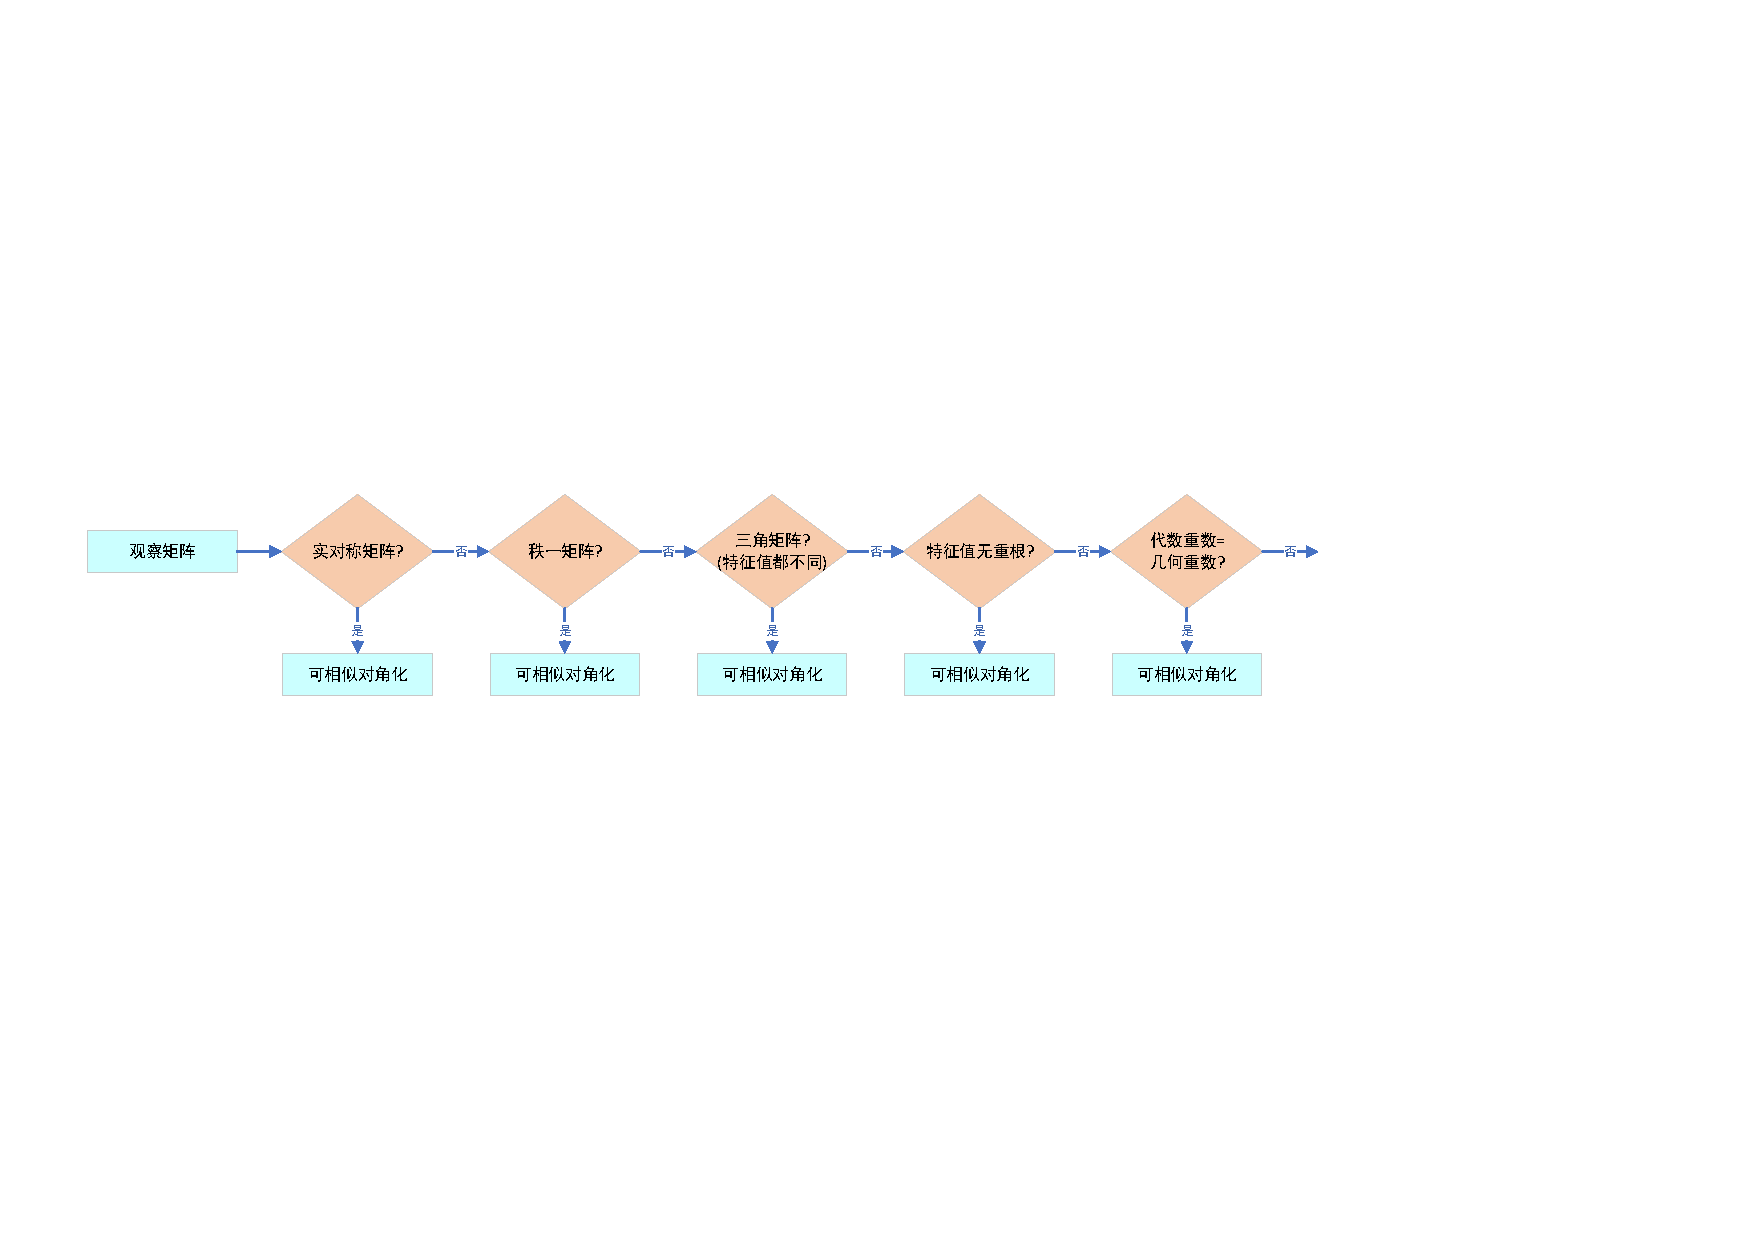
\includegraphics[scale=0.6]{figures/sdcjz.pdf}
%     \caption{}
%     \label{figure:sdcjz}
% \end{figure}

\begin{example}[2004 数一]
    设矩阵 $\vb*{A}=\mqty(1&2&-3\\-1&4&-3\\1&a&5)$ 的特征方程有一个二重根,求 $a$ 的值,并讨论 $\vb*{A}$ 是否可相似对角化.
\end{example}
\begin{solution}
    $|\lambda\vb*{E}-\vb*{A}|=\mqty|\lambda-1&-2&3\\1&\lambda-4&3\\-1&-a&\lambda-5|\xlongequal[r_2+r_3]{r_1-r_2}\mqty|\lambda-2&2-\lambda&0\\0&\lambda-4-a&\lambda-2\\-1&-a&\lambda-5|=(\lambda-2)\qty[(\lambda-5)(\lambda-4-a)+(\lambda-2)(1+a)]$,
    当 $\lambda=2$ 是方程的二重根时,则有 $(2-5)(2-4-a)=0\Rightarrow a=-2$,于是 $\vb*{A}=\mqty(1&2&-3\\-1&4&-3\\1&-2&5)$,此时,
    $$\rank(2\vb*{E}-\vb*{A})=\rank\mqty(1&-2&3\\1&-2&3\\-1&2&-3)=\rank\mqty(0&0&0\\0&0&0\\-1&2&-3)=1=3-2$$
    因此可以相似对角化; 当 $2$ 不是方程的二重根时,$[(\lambda-5)(\lambda-4-a)+(\lambda-2)(1+a)]$ 为完全平方数,解得 $a=-\dfrac{2}{3}$,此时 $4$ 是该方程的二重根,
    于是 $\vb*{A}=\mqty(1&2&-3\\-1&4&-3\\1&-\dfrac{2}{3}&5)$,$\rank(4\vb*{E}-\vb*{A})\neq 1$,于是 $a=-\dfrac{2}{3}$ 时,$\vb*{A}$ 不能相似对角化.
\end{solution}

\begin{example}
    设矩阵 $\vb*{A}=\mqty(0&1&0&0\\1&0&0&0\\0&0&y&1\\0&0&1&2)$
    \begin{enumerate}[label=(\arabic{*})]
        \item 已知 $\vb*{A}$ 的一个特征值为 3,求 $y$;
        \item 求矩阵 $\vb*{P}$,使得 $\vb*{AP}^{\top}(\vb*{AP})$ 为对角矩阵.
    \end{enumerate}
\end{example}
\begin{solution}
    \begin{enumerate}[label=(\arabic{*})]
        \item 因为 $$|\lambda\vb*{E}-\vb*{A}|=\mqty|\lambda&-1&0&0\\-1&\lambda&0&0\\0&0&\lambda-y&-1\\0&0&-1&\lambda-2|=\mqty|\lambda&-1\\-1&\lambda|\cdot\mqty|\lambda-y&-1\\-1&\lambda-2|=\qty(\lambda^2-1)[(\lambda-y)(\lambda-2)-1]=0$$
              将 $\lambda=3$ 代入得,$y=2$.
        \item 由 (1) 可知 $\vb*{A}=\mqty(0&1&0&0\\1&0&0&0\\0&0&2&1\\0&0&1&2)$,那么 $\vb*{A}^\top=\vb*{A}$,得 $(\vb*{AP})^\top(\vb*{AP})=\vb*{P}^\top\vb*{A}^2\vb*{P}$,
              而 $\vb*{A}^2=\mqty(1&0&0&0\\0&1&0&0\\0&0&5&4\\0&0&4&5)$,由 $|\lambda\vb*{E}-\vb*{A}^2|=0$ 解得 $\lambda_1=1$ (三重),$\lambda_2=9$,对应 $\lambda_1=1$ 的特征向量为
              $$\vb*{\alpha}_1=(1,0,0,0)^\top\text{,}\vb*{\alpha}_2=(0,1,0,0)^\top\text{,}\vb*{\alpha}_3=(0,0,-1,1)^\top$$
              标准正交化得 $$\vb*{\beta}_1=(1,0,0,0)^\top\text{,}\vb*{\beta}_2=(0,1,0,0)^\top\text{,}\vb*{\beta}_3=\dfrac{1}{\sqrt{2}}(0,0,-1,1)^\top$$
              对应于 $\lambda_2=9$ 的特征向量为 $\vb*{\alpha}_4=(0,0,1,1)^\top$,经过单位化后,$\vb*{\beta}_4=\dfrac{1}{\sqrt{2}}(0,0,1,1)^\top$,于是
              $$\vb*{P}=(\vb*{\beta}_1,\vb*{\beta}_2,\vb*{\beta}_3,\vb*{\beta}_4)=\mqty(1&0&0&0\\0&1&0&0\\0&0&-\dfrac{1}{\sqrt{2}}&\dfrac{1}{\sqrt{2}}\\[6pt]0&0&\dfrac{1}{\sqrt{2}}&\dfrac{1}{\sqrt{2}})\text{,}(\vb*{AP})^\top(\vb*{AP})=\mqty(\dmat{1,1,1,9}).$$
    \end{enumerate}
\end{solution}

\begin{example}
    设矩阵 $\vb*{A}=\mqty(1& -1& 1\\ x& 4& y\\ -3& -3& 5)$ 有 $3$ 个线性无关的特征向量,且 $\lambda=2$ 是 $\vb*{A}$ 的二重特征值.
    \begin{enumerate}[label=(\arabic{*})]
        \item 求 $x\text{,}y$ 的值;
        \item 求可逆矩阵 $\vb*{P}$,使得 $\vb*{P}^{-1}\vb*{AP}$ 为对角矩阵.
    \end{enumerate}
\end{example}
\begin{solution}
    \begin{enumerate}[label=(\arabic{*})]
        \item 根据题设,$\vb*{A}$ 有 3 个线性无关的特征向量,所以 $\vb*{A}$ 可对角化,$\vb*{A}$ 的任一特征值的几何重数与代数重数相等,对于特征值 $\lambda=2$ (二重),$\vb*{A}$
              有两个线性无关的特征向量,由此可知 $\rank(2\vb*{E}-\vb*{A})=1$,利用初等行变化,得
              $$2\vb*{E}-\vb*{A}=\mqty(\dmat{2,2,2})-\mqty(1 &-1 &1\\ x &4 &y\\ -3 &-3 &5)=\mqty(1 &1 &-1\\ -x &-2 &-y\\ 3 &3 &-3)\xrightarrow[r_3-3r_1]{r_2+r_1\cdot x}\mqty(1 &1 &-1\\ 0 &x-2 &-y-x\\ 0 &0 &0)$$
              因此,有 $x=2\text{,}y=-2.$
        \item 由 (1) 可知,$\vb*{A}=\mqty(1 &-1 &1\\ 2 &4 &-2\\ -3 &-3 &5)$,那么矩阵 $\vb*{A}$ 的特征多项式为
              $$f(\lambda)=|\lambda\vb*{E}-\vb*{A}|=\mqty|\lambda-1 &1 &-1\\ -2 &\lambda-4 &2\\ 3 &3 &\lambda-5|\xlongequal[r_3-3r_1]{r_2+2r_1}\mqty|\lambda-1 &1 &-1\\ 2\lambda-4 &\lambda-2 &0\\ 6-3\lambda &0 &\lambda-2|=(\lambda-2)(\lambda-6)$$
              解得 $\lambda_1=\lambda_2=2\text{,}\lambda_3=6$,对于特征值 $\lambda_{1,2}=2$,解齐次方程组 $(2\vb*{E}-\vb*{A})\vb*{x}=\vb*{0}$,对应的特征向量为
              $\vb*{\alpha}_1=(1,-1,0)^\top\text{,}\vb*{\alpha}_2=(1,0,1)^\top$,
              对于特征值 $\lambda_{3}=6$,解齐次方程组 $(6\vb*{E}-\vb*{A})\vb*{x}=\vb*{0}$,对应的特征向量为
              $\vb*{\alpha}_3=(1,-2,3)^\top$,
              令 $\vb*{P}=(\vb*{\alpha}_1,\vb*{\alpha}_2,\vb*{\alpha}_3)=\mqty(1 &1 &1\\ -1 &0 &-2\\ 0 &1 &3)$,则 $\vb*{P}^{-1}\vb*{AP}=\mqty(\dmat{2,2,6})$ 为对角矩阵.
    \end{enumerate}
\end{solution}

\section{方阵的幂}

\begin{definition}[方阵的幂]
    对 $ n $ 阶方阵 $ A $,定义
    $\displaystyle\vb*{A}^{k}=\underbrace{\vb*{A} \cdot \vb*{A} \cdot \cdots \cdot \vb*{A}}_{k \text{个}}$,
    称为 $ \vb*{A} $ 的 $ k $ 次幂.
\end{definition}

\begin{example}
    设 $\vb*{A}=\mqty(\dfrac{2}{3}&-\dfrac{1}{3}&-\dfrac{1}{3}\\[6pt]-\dfrac{1}{3}&\dfrac{2}{3}&-\dfrac{1}{3}\\[6pt]-\dfrac{1}{3}&-\dfrac{1}{3}&\dfrac{2}{3})$,求 $\vb*{A}^9$.
\end{example}
\begin{solution}
    $\vb*{A}^2=\mqty(\dfrac{2}{3}&-\dfrac{1}{3}&-\dfrac{1}{3}\\[6pt]-\dfrac{1}{3}&\dfrac{2}{3}&-\dfrac{1}{3}\\[6pt]-\dfrac{1}{3}&-\dfrac{1}{3}&\dfrac{2}{3})^{2}=\dfrac{1}{9}\mqty(6&-3&-3\\-3&6&-3\\-3&-3&6)=\vb*{A}$,因此 $\vb*{A}^9=\vb*{A}\qty(\vb*{A}^2)^4=\vb*{A}\vb*{A}^4=\vb*{A}\qty(\vb*{A}^2)^2=\vb*{A}^2=\vb*{A}.$
\end{solution}

\subsection{利用方阵的迹求解}

\begin{theorem}[秩一矩阵的幂]
    当 $\vb*{A}$ 为方阵且秩 $\rank\vb*{A}=1$,则 $\vb*{A}^n=\qty[\tr(\vb*{A})]^{n-1}\vb*{A}$.
\end{theorem}

\begin{example}
    设 $\vb*{A}=\mqty(a&b&c&d\\2a&2b&2c&2d\\3a&3b&3c&3d\\4a&4b&4c&4d)~  (a,b,c,d)$ 不全为 0,求解 $\vb*{A}^n.$
\end{example}
\begin{solution}
    显然 $\rank\vb*{A}=1$,则 $$\vb*{A}^n=\qty[\tr(\vb*{A})]^{n-1}\vb*{A}=(a+2b+3c+4d)^{n-1}\vb*{A}.$$
\end{solution}

\begin{example}
    设 $\vb*{A}=\mqty(0&0&1\\0&1&0\\1&0&0)$,已知矩阵 $\vb*{B}$ 与矩阵 $\vb*{A}$ 相似,求
    $\rank(\vb*{B}-2\vb*{E})+\rank(\vb*{B}-\vb*{E})$,及 $(\vb*{A}-\vb*{E})^n$,$n$ 为大于 1 的正整数.
\end{example}
\begin{solution}
    因为 $\vb*{B}\sim\vb*{A}$,所以
    \begin{flalign*}
        \rank(\vb*{B}-2\vb*{E})+\rank(\vb*{B}-\vb*{E}) & =\rank(\vb*{A}-2\vb*{E})+\rank(\vb*{A}-\vb*{E})=\rank\mqty(-2 & 0 & 1 \\0&-1&0\\1&0&-2)+\rank\mqty(-1&0&1\\0&0&0\\1&0&-1)\\
                                                       & =3+1=4
    \end{flalign*}
    因为 $\rank(\vb*{A}-\vb*{E})=1$,所以 $(\vb*{A}-\vb*{E})^n=\qty[\tr(\vb*{A}-\vb*{E})\vb*{A}]^{n-1}(\vb*{A}-\vb*{E})=(-2)^{n-1}\mqty(-1&0&1\\0&0&0\\1&0&-1).$
\end{solution}

\subsection{利用幂零矩阵求解}

\begin{example}
    设 $\vb*{A}=\mqty(0&1&2&3\\0&0&2&3\\0&0&0&3\\0&0&0&0)$,求解 $\vb*{A}^n.$
\end{example}
\begin{solution}
    因为 $\vb*{A}^4=\vb*{O}$,并且
    \begin{flalign*}
        \vb*{A}^2=\mqty(0 & 1 & 2 & 3 \\0&0&2&3\\0&0&0&3\\0&0&0&0)\cdot\mqty(0&1&2&3\\0&0&2&3\\0&0&0&3\\0&0&0&0)=\mqty(0&0&2&9\\0&0&0&6\\0&0&0&0\\0&0&0&0)\\
        \vb*{A}^3=\mqty(0 & 0 & 2 & 9 \\0&0&0&6\\0&0&0&0\\0&0&0&0)\cdot \mqty(0&1&2&3\\0&0&2&3\\0&0&0&3\\0&0&0&0)=\mqty(0&0&2&9\\0&0&0&6\\0&0&0&0\\0&0&0&0)
    \end{flalign*}
\end{solution}

\subsection{利用二项式展开求解}

\begin{example}
    设 $\vb*{A}=\begin{pmatrix}
            1 & 3 \\
            0 & 1
        \end{pmatrix}$,求 $\vb*{A}^n$.
\end{example}
\begin{solution}
    由 $\vb*{A}=\begin{pmatrix}
            1 & 3 \\
            0 & 1
        \end{pmatrix}=\begin{pmatrix}
            1 & 0 \\
            0 & 1
        \end{pmatrix}+\begin{pmatrix}
            0 & 3 \\
            0 & 0
        \end{pmatrix}=\vb*{E}+\vb*{B}$,而
    $\displaystyle\vb*{B}^2=\begin{pmatrix}
            0 & 3 \\
            0 & 0
        \end{pmatrix}\begin{pmatrix}
            0 & 3 \\
            0 & 0
        \end{pmatrix}=\mathrm{0}$,
    所以当 $k\geqslant2$ 时,有 $\vb*{B}^k=\mathrm{0}$,
    而单位矩阵 $\vb*{E}$ 与任意矩阵可换,由二项式定理,得
    \begin{flalign*}
        \vb*{A}^n & =(\vb*{E}+\vb*{B})^n=\sum_{k=0}^{n}\mathrm{C}_n^k\vb*{E}^{n-k}\vb*{B}^k=\vb*{E}^n+\mathrm{C}_n^1\vb*{E}^{n-1}B \\
                  & =\begin{pmatrix}
                         1 & 0 \\
                         0 & 1
                     \end{pmatrix}+n\begin{pmatrix}
                                        1 & 0 \\
                                        0 & 1
                                    \end{pmatrix}\begin{pmatrix}
                                                     0 & 3 \\
                                                     0 & 0
                                                 \end{pmatrix}=\begin{pmatrix}
                                                                   1 & 3n \\
                                                                   0 & 1
                                                               \end{pmatrix}.
    \end{flalign*}
\end{solution}

\begin{example}[2002 复旦大学]
    证明: $$\begin{pmatrix}
            \dfrac{3}{2} & -\dfrac{1}{2} \\[6pt]
            \dfrac{1}{2} & \dfrac{1}{2}
        \end{pmatrix}^{100}=\begin{pmatrix}
            51 & -50 \\
            50 & -49
        \end{pmatrix}.$$
\end{example}
\begin{proof}[{\songti \textbf{证}}]
    注意到 \begin{flalign*}
        \begin{pmatrix}
            \dfrac{3}{2} & -\dfrac{1}{2} \\[6pt]
            \dfrac{1}{2} & \dfrac{1}{2}
        \end{pmatrix}=\begin{pmatrix}
                          1 & 0 \\
                          0 & 1
                      \end{pmatrix}+\begin{pmatrix}
                                        \dfrac{1}{2} & -\dfrac{1}{2} \\[6pt]
                                        \dfrac{1}{2} & -\dfrac{1}{2}
                                    \end{pmatrix}=\begin{pmatrix}
                                                      1 & 0 \\
                                                      0 & 1
                                                  \end{pmatrix}+\begin{pmatrix}
                                                                    \dfrac{1}{2} \\[6pt]
                                                                    \dfrac{1}{2}
                                                                \end{pmatrix}(1,-1) =\vb*{E}+\vb*{\alpha}\vb*{\beta}^{\top}
    \end{flalign*}
    其中 $\vb*{E}$ 是二阶单位矩阵,$\vb*{\alpha}=\qty(\dfrac{1}{2},\dfrac{1}{2})^{\top}$,$\vb*{\beta}=(1,-1)^{\top}$,并且 $\vb*{\beta}\vb*{\alpha}^T=0$,所以
    $$\qty(\vb*{\alpha\beta}^\top)^2=\qty(\vb*{\alpha\beta}^{\top})\qty(\vb*{\alpha\beta}^{\top})=\vb*{\alpha}\qty(\vb*{\beta}^{\top}\vb*{\alpha})\vb*{\beta}^{\top}=\vb*{O}$$
    于是 \begin{flalign*}
        \begin{pmatrix}
            \dfrac{3}{2} & -\dfrac{1}{2} \\[6pt]
            \dfrac{1}{2} & \dfrac{1}{2}
        \end{pmatrix}^{100} & =\qty(\vb*{E}+\vb*{\alpha}\vb*{\beta}^{\top})^{100}=\sum_{k=0}^{100}\mathrm{C}_{100}^k\qty(\vb*{\alpha\beta}^\top)^k=\vb*{E}+100\vb*{\alpha\beta}^{\top} \\
                                             & =\begin{pmatrix}
                                                    1 & 0 \\
                                                    0 & 1
                                                \end{pmatrix}+100\begin{pmatrix}
                                                                     1 \\1
                                                                 \end{pmatrix}(1,-1)=\begin{pmatrix}
                                                                                         51 & -50 \\
                                                                                         50 & -49
                                                                                     \end{pmatrix}.
    \end{flalign*}
\end{proof}

\subsection{Cayley-Hamilton 定理}

\begin{theorem}[Cayley-Hamilton]
    设 $n$ 阶方阵 $\vb*{A}$ 的特征多项式为 $\varphi(\lambda)=\lambda^n+a_{n-1}\lambda^{n-1}+\cdots+a_1\lambda+a_0$,则 $$\varphi(\vb*{A})=\vb*{A}^n+a_{n-1}\vb*{A}^{n-1}+\cdots++a_1\vb*{A}+a_0\vb*{E}_n=\vb*{O}.$$
\end{theorem}

\subsection{矩阵幂转化}

\begin{example}
    设 $\vb*{A}=\mqty(\underline{1}&3&-1\\0&\underline{4}&5\\0&0&\underline{9})$,求\textbf{一个}矩阵 $\vb*{B}$ 使得 $\vb*{B}^2=\vb*{A}.$
\end{example}
\begin{solution}
    因为 $\vb*{A}$ 是一上三角矩阵,那么 $\vb*{A}$ 的特征值分别为 $\lambda_1=1,~\lambda_2=4,~\lambda_3=9$,所以 $\vb*{A}$ 一定能相似对角化,
    因此存在一可逆实矩阵 $\vb*{P}$,使得 $\vb*{P}^{-1}\vb*{AP}=\diag(1,4,9)$,易得 $\lambda_1$ 对于的特征向量为 $\vb*{\xi}_1=(1,0,0)^\top$; $\lambda_2$ 对应的特征向量为 $\vb*{\xi}_2=(1,1,0)^\top$;
    $\lambda_3$ 对应的特征向量为 $\vb*{\xi}_3=(1,4,4)^\top$,则取 $\vb*{P}=(\vb*{\xi}_1,\vb*{\xi}_2,\vb*{\xi}_3)$,于是 
    $$\vb*{A}=\vb*{P}\diag(1,4,9)\vb*{P}^{-1}=\vb*{P}\diag((\pm1)^2,(\pm2)^2,(\pm3)^2)\vb*{P}^{-1}=\vb*{P\Lambda P}^{-1}\vb*{P\Lambda P}^{-1}\Rightarrow \vb*{B}=\vb*{P\Lambda P}^{-1}$$
    因此 $\vb*{B}=\mqty(1&1&1\\0&1&4\\0&0&4)\mqty(\dmat{1,2,3})\mqty(1&-1&\dfrac{3}{4}\\[6pt]0&1&-1\\0&0&\dfrac{1}{4})=\mqty(1&1&-\dfrac{1}{2}\\[6pt]0&2&1\\0&0&3).$
\end{solution}

%\section{不变子空间}

\chapter{二次型}%============================14

\begin{flushright}
    \begin{tabular}{r||}
        \textit{“数学是一种无限的创造力, 它能够解释和预测自然界的现象。”}\\
        ——\textit{欧拉}
    \end{tabular}
\end{flushright}

二次型在数学和应用领域中有广泛的应用和重要性. 它可以用于描述几何对象的性质、最优化问题的求解、物理学中的能量和动能等物理量、统计学中的数据分析和建模, 以及工程和控制系统中的应用等. 通过对二次型进行矩阵分析和特征值分解等方法, 可以得到二次型的特性和解决各种问题. 
%\section{二次型的规范形与标准形}

1. 二次型的规范形:

如果一个二次型经过合适的线性变换可以化为对角形式, 即对角元素非零, 其他元素为零, 那么这个对角形式就是二次型的规范形. 规范形可以表示为:
$$
q(\vb*{x}) = \vb*{x}^{\top} \vb*{A x} = \lambda_1 x_1^2 + \lambda_2 x_2^2 + \ldots + \lambda_n x_n^2
$$
其中 $\lambda_1, \lambda_2, \ldots, \lambda_n$ 是对角矩阵 $A$ 的特征值. 

2. 二次型的标准形:

如果一个二次型经过合适的线性变换可以化为更简单的形式, 即对角元素为 $\pm 1$, 其他元素为零, 那么这个形式就是二次型的标准形. 标准形可以表示为:
$$
q(\vb*{x}) = \vb*{x}^{\top} \vb*{A x} = x_1^2 + x_2^2 + \ldots + x_r^2 - x_{r+1}^2 - \ldots - x_n^2
$$
其中 $r$ 是矩阵 $\vb*{A}$ 的正特征值的个数. 

\subsection{二次型的基本概念}

\begin{definition}[$n$ 元二次型]
    含有 $ n $ 个变量 $ x_{1}, x_{2}, \cdots, x_{n} $ 的二次齐次函数
    $$\begin{aligned}
            f\left(x_{1}, x_{2}, \cdots, x_{n}\right)= & a_{11} x_{1}^{2}+a_{22} x_{2}^{2}+\cdots+a_{n n} x_{n}^{2}+2 a_{12} x_{1} x_{2}+2 a_{13} x_{1} x_{3}+\cdots+ \\
                                                       & 2 a_{1 n} x_{1} x_{n}+2 a_{23} x_{2} x_{3}+\cdots+2 a_{2 n} x_{2} x_{n}+\cdots+                              \\
                                                       & 2 a_{n-1, n} x_{n-1} x_{n}
        \end{aligned}$$
    称为 $ n $ \textit{元二次型}.
\end{definition}

常见的三元二次型:
$$f\left(x_{1}, x_{2}, x_{3}\right)= a x_{1}^{2}+b x_{2}^{2}+c x_{3}^{2}+d x_{1} x_{2}+e x_{3} x_{2}+f x_{1} x_{3}$$
几何意义: 三元二次型的几何图形是空间曲面.

二次型有矩阵表示.

\begin{definition}[二次型的矩阵表达]
    在二次型表达式中取 $ a_{i j}=a_{j i} $, 则
    $$2 a_{i j} x_{i} x_{j}=a_{i j} x_{i} x_{j}+a_{j i} x_{j} x_{i}$$
    于是上述二次型可以写为
    $$f\left(x_{1}, x_{2}, \cdots, x_{n}\right)=\sum_{i=1}^{n} \sum_{j=1}^{n} a_{i j} x_{i} x_{j}=
        \left(x_{1}, x_{2}, \cdots, x_{n}\right)
        \mqty(a_{11} & a_{12} & \cdots & a_{1 n} \\
        a_{21} & a_{22} & \cdots & a_{2 n} \\
        \vdots & \vdots & & \vdots \\
        a_{n 1} & a_{n 2} & \cdots & a_{n n})
        \mqty(x_{1} \\    x_{2} \\    \vdots \\    x_{n})
        =\vb*{x}^\top \vb*{A} \vb*{x} $$
    或
    $$f(x_1,x_2,\cdots,x_n)=a\sum_{i=1}^{n}x_i^2+2b\sum_{1\leqslant j<k\leqslant n}x_jx_k=
        \left(x_{1}, x_{2}, \cdots, x_{n}\right)
        \mqty(a & b & \cdots & b \\
        b & a & \cdots & b \\
        \vdots & \vdots & & \vdots \\
        b & b & \cdots & a)
        \mqty(x_{1} \\    x_{2} \\    \vdots \\    x_{n})
        =\vb*{x}^\top \vb*{A} \vb*{x}$$
    其中 $ \vb*{A} $ 是对称矩阵, 称为\textit{二次型} $ f $ \textit{的矩阵},
    矩阵 $ \vb*{A} $ 的秩称为\textit{二次型} $ f $ \textit{的秩}.
\end{definition}

\begin{example}
    二次型 $$f(x_1,x_2,x_3)=x_1^2+ax_2^2+x_3^2+2x_1x_2+2ax_1x_3+2x_2x_3$$ 的秩为 $2$, 求 $a.$
\end{example}
\begin{solution}
    二次型 $f$ 矩阵为 $\vb*{A}=\mqty(1&1&a\\1&a&1\\a&1&1)$, 由题意 $\rank\vb*{A}=2\Rightarrow \det\vb*{A}=0\Rightarrow a=-2.$
\end{solution}

\begin{definition}[二次型的标准形]
    如果二次型中只含有变量的平方项, 所有混合项 $ x_{i} x_{j}(i \neq j) $ 的系数全是零, 即
    $$\vb*{x}^{\top} A \vb*{x}=d_{1} x_{1}^{2}+d_{2} x_{2}^{2}+\cdots+d_{n} x_{n}^{2}$$
    这样的二次型称为\textit{标准形}.
\end{definition}

\begin{definition}[二次型的规范形]
    在标准形中, 如平方项的系数 $ d_{j} $ 为 $ 1,-1 $ 或 $0$,
    $$\vb*{x}^{\top} \vb*{A} \vb*{x}=x_{1}^{2}+x_{2}^{2}+\cdots+x_{p}^{2}-x_{p+1}^{2}-\cdots-x_{p+q}^{2}$$
    则称其为二次型的\textit{规范形}.
\end{definition}

\begin{example}
    化二次型 $f=2x_2^2+2x_1x_3$ 为标准形, 并写出所用坐标变换.
\end{example}
\begin{solution}
    $f=2x_2^2+\dfrac{1}{2}(x_1+x_3)^2-\dfrac{1}{2}(x_1-x_3)^2$, 令
    $\begin{cases}
            z_1=\sqrt2x_2                  \\
            z_2=\dfrac{1}{\sqrt2}(x_1+x_3) \\[6pt]
            z_3=\dfrac{1}{\sqrt2}(x_1-x_3)
        \end{cases}$ 则 $\vb*{x}=\vb*{Cz}$, 
    其中 $\vb*{C}=\mqty(0&\dfrac{1}{\sqrt2}&\dfrac{1}{\sqrt2}\\[6pt]\dfrac{1}{\sqrt2}&0&0\\[6pt]0&\dfrac{1}{\sqrt{2}}&\dfrac{1}{\sqrt{2}}).$
\end{solution}

\begin{example}
    将二次型 $$f(x_1,x_2,x_3)=x_1^2+3x_2^2+3x_3^2+2x_1x_2-4x_1x_3$$ 化为标准形, 并写出所用坐标变换.
\end{example}
\begin{solution}
    $f$ 的标准形为 $$f(x_1,x_2,x_3)=(x_1+x_2-2x_3)^2+2(x_2+x_3)^2-3x_3^2$$
    故令 $\left\{\begin{matrix}
            z_1 & = & x_1 & + & x_2 & - & 2x_3 \\
            z_2 & = &     &   & x_2 & + & x_3  \\
            z_3 & = &     &   &     &   & x_3
        \end{matrix}\right.$ 即坐标变换 $\left\{\begin{matrix}
            x_1 & = & z_1 & - & z_2 & + & 3z_3 \\
            x_2 & = &     &   & z_2 & - & z_3  \\
            x_3 & = &     &   &     &   & z_3
        \end{matrix}\right.$, 或 $\vb*{x}=\mqty(1&-1&3\\0&1&-1\\0&0&1)\vb*{z}$, 则有 $f=z_1^2+2z_2^2-3z_3^2.$
\end{solution}

\begin{example}
    已知二次型 \label{fx1x2x3gy1y2y3}$$f(x_1,x_2,x_3)=x_1^2+2x_2^2+2x_3^2+2x_1x_2-2x_1x_3,~g(y_1,y_2,y_3)=y_1^2+y_2^2+y_3^2+2y_2y_3$$
    求可逆变换 $\vb*{x}=\vb*{Py}$ 将 $f$ 化为 $g.$
\end{example}
\begin{solution}
    $f$ 的标准形为 $$f(x_1,x_2,x_3)=(x_1+x_2-x_3)^2+(x_2+x_3)^2$$
    故令 $\left\{\begin{matrix}
            z_1 & = & x_1 & + & x_2 & - & x_3 \\
            z_2 & = &     &   & x_2 & + & x_3 \\
            z_3 & = &     &   &     &   & x_3
        \end{matrix}\right.\Rightarrow \left\{\begin{matrix}
            x_1 & = & z_1 & - & z_2 & + & 2z_3 \\
            x_2 & = &     &   & z_2 & - & z_3  \\
            x_3 & = &     &   &     &   & z_3
        \end{matrix}\right.$, 则 $\vb*{x}=\vb*{P}_1\vb*{z}$, 其中 $\vb*{P}_1=\mqty(1&-1&2\\0&1&-1\\0&0&1)$
    同理 $g(x_1,x_2,x_3)=y_1^2+(y_2+y_3)^2$, 令 $\left\{\begin{matrix}
            z_1 & = & y_1                 \\
            z_2 & = &     & y_2 & + & y_3 \\
            z_3 & = &     &     &   & y_3
        \end{matrix}\right.$ 即 $\vb*{z}=\vb*{P}_2\vb*{y}$, 其中 $\vb*{P}_2=\mqty(1&0&0\\0&1&1\\0&0&1)$
    于是 $$\vb*{x}=\vb*{P}_1\vb*{P}_2\vb*{y}=\mqty(1&-1&1\\0&1&0\\0&0&1)\vb*{y}$$
    故 $\vb*{P}=\mqty(1&-1&1\\0&1&0\\0&0&1).$
\end{solution}

\begin{definition}[正负惯性指数]
    在二次型 $ \vb*{x}^{\top} \vb*{A} \vb*{x} $ 的规范形中, 正的平方项的个数 $ p $ 称为\textit{二次型的正惯性指数}, 负的平方项的个数 $ q $ 称为\textit{二次型的负惯性指数}.
\end{definition}

\begin{definition}[符号差]
    正惯性指数 $p$ 与负惯性指数 $q$ 的差称为符号差 $s$, 即 $s=p-q.$
\end{definition}
\begin{example}
    设 $f(x_1,x_2,x_3)=ax_1^2+(a-1)x_2^2+(a+2)x_3^2$ 的标准形是 $y_1^2-y_2^2-y_3^2$, 求 $a$ 的取值范围.
\end{example}
\begin{solution}
    由题意可知 $p=1,q=2$, 于是 $a-1<a<0<a+2\Rightarrow -2<a<0.$
\end{solution}

\begin{example}
    设 $\vb*{A}$ 是 $n$ 阶实对称矩阵, 秩为 $r$, 符号差为 $s$, 则必有 (\quad).
    \begin{tasks}(2)
        \task $r$ 是奇数, $s$ 是偶数
        \task $s$ 是奇数, $r$ 是偶数
        \task $r,s$ 均为偶数
        \task $r,s$ 或均为奇数或均为偶数
    \end{tasks}
\end{example}
\begin{solution}
    $r=p+q,s=p-q$, 那么 $r+s=2p$, 从而 $r,s$ 或均为奇数或均为偶数.
\end{solution}

\begin{example}
    求二次型 $$\displaystyle f(x_1,x_2,\cdots,x_n)=(n-1)\sum_{i=1}^{n}x_i^2-2\sum_{1\leqslant j<k\leqslant n}x_jx_k$$
    的符号差.
\end{example}
\begin{solution}
    设此二次型的矩阵为 $\vb*{A}$, 则 $$\vb*{A}=\mqty(n-1&-1&-1&\cdots&-1\\-1&n-1&-1&\cdots&-1\\\vdots& \vdots& \vdots& \ddots & \vdots\\-1&-1&-1&\cdots&n-1)$$
    且 $|\lambda\vb*{E}-\vb*{A}|=\lambda(\lambda-n)^{n-1}$ (参考例题 \ref{ascendingMethod}(2) 的解法), 所以 $\vb*{A}$ 的特征值为 $\lambda_1=\lambda_2=\cdots=\lambda_{n-1}=n,\lambda_n=0$, 故符号差 $s=n-1.$
\end{solution}

\begin{definition}[非线性替换]
    如果
    \begin{equation}
        \left\{\begin{array}{l}
            x_{1}=c_{11} y_{1}+c_{12} y_{2}+\cdots+c_{1 n} y_{n}, \\
            x_{2}=c_{21} y_{1}+c_{22} y_{2}+\cdots+c_{2 n} y_{n}  \\
            \cdots                                                \\
            x_{n}=c_{n 1} y_{1}+c_{n 2} y_{2}+\cdots \cdots+c_{n n} y_{n}
        \end{array}\right.
        \tag{*}
    \end{equation}
    满足 $$|\vb*{C}|=\mqty|c_{11}  & c_{12}  & \cdots & c_{1 n} \\
            c_{21}  & c_{22}  & \cdots & c_{2 n} \\
            \vdots  & \vdots  &        & \vdots  \\
            c_{n 1} & c_{n 2} & \cdots & c_{n n}| \neq 0$$
    称 (*) 为由 $ \vb*{x}=\left(x_{1}, x_{2}, \cdots, x_{n}\right)^{\top} $ 到 $ \vb*{y}=\left(y_{1}, y_{2}, \cdots, y_{n}\right)^{\top} $ 的\textit{非退化线性替换}, 且 (*) 可用矩阵描述, 即
    $$\mqty( x_{1}  \\
                x_{2}  \\
                \vdots \\
                x_{n})=\mqty(c_{11}  & c_{12}  & \cdots & c_{1 n} \\
                c_{21}  & c_{22}  & \cdots & c_{2 n} \\
                \vdots  & \vdots  &        & \vdots  \\
                c_{n 1} & c_{n 2} & \cdots & c_{n n})
                \mqty(y_{1}  \\
                y_{2}  \\
                \vdots \\
                y_{n})$$
    或 $ \vb*{x}=\vb*{C y} $, 其中 $ \vb*{C} $ 是可逆矩阵.
\end{definition}

如果没有特别说明, 本章所涉及的二次型均为实二次型, 即二次型中变量的系数均为实数, 所涉及的矩阵和向量都是实的.

\subsection{二次型的常用结论}

\begin{enumerate}[label=(\arabic{*})]
    \item 二次型与对称矩阵一一对应.
    \item 变量 $ \vb*{x}=\left(x_{1}, x_{2}, \cdots, x_{n}\right)^{\top} $ 的 $ n $ 元二次型 $ \vb*{x}^{\top} \vb*{A} \vb*{x} $ 经过非退化线性替换 $ \vb*{x}=\vb*{C} \vb*{y} $ 后, 成为变量 $ \vb*{y}=\left(y_{1}, y_{2}, \cdots, y_{n}\right)^{\top} $ 的 $ n $ 元二次型 $ \vb*{y}^{\top} \vb*{B} \vb*{y} $, 其中 $ \vb*{B}=\vb*{C}^{\top} \vb*{A} \vb*{C} $.
    \item 任意的 $ n $ 元二次型 $ \vb*{x}^{\top} \vb*{A} \vb*{x} $ 都可以通过非退化线性替换化成标准形 $ d_{1} y_{1}^{2}+   d_{2} y_{2}^{2}+\cdots+d_{n} y_{n}^{2} $, 其中 $ d_{i}(i=1,2, \cdots, n) $ 是实数.
    \item 任意 $ n $ 元二次型 $ \vb*{x}^{\top} \vb*{A} \vb*{x} $, 由于 $ \vb*{A} $ 是实对称矩阵, 故必存在正交变换 $ \vb*{x}=\vb*{Q} \vb*{y}$ ($\vb*{Q} $ 为正交矩阵), 使得二次型化为标准形 $ \lambda_{1} y_{1}^{2}+\lambda_{2} y_{2}^{2}+\cdots+\lambda_{n} y_{n}^{2} $, 且 $ \lambda_{1}, \lambda_{2}, \cdots, \lambda_{n} $ 是 $ A $ 的 $ n $ 个特征值.
    \item 非退化线性替换保持二次型的正负惯性指数、秩、正定性等.
\end{enumerate}

\begin{theorem}[惯性定理]
    任意 $n$ 元二次型 $\vb*{x}^\top\vb*{Ax}$ 都可通过非退化线性替换化为规范形
    $$z_1^2+z_2^2+\cdots+z_p^2-z_{p+1}^2-\cdots-z_{p+q}^2$$
    其中 $p$ 为正惯性指数, $q$ 为负惯性指数, $p+q$ 为二次型的秩, 且 $p$, $q$ 由二次型唯一确定, 即规范形是唯一的.
\end{theorem}

\begin{example}
    二次型 $f(x_1,x_2,x_3)=\vb*{x}^\top\vb*{Ax}$, 其中 $\vb*{A}=\mqty(1&2&2\\0&2&\dfrac{1}{2}\\[6pt]0&\dfrac{7}{2}&1)$, 求 $f$ 的正惯性系数.
\end{example}
\begin{solution}
    实对称矩阵 $\vb*{A}_0=\dfrac{1}{2}\qty(\vb*{A}+\vb*{A}^\top)=\dfrac{1}{2}\qty(\mqty(1&2&2\\0&2&\dfrac{1}{2}\\[6pt]0&\dfrac{7}{2}&1)+\mqty(1&0&0\\2&2&\dfrac{7}{2}\\[6pt]2&\dfrac{1}{2}&1))=\mqty(1&1&1\\1&2&2\\1&2&1)$, 
    设 $\vb*{A}_0$ 的特征值为 $\lambda_1,~\lambda_2,~\lambda_3$ 则 $$\begin{cases}
            \lambda_1+\lambda_2+\lambda_3=\tr\vb*{A}_0=4 \\
            \lambda_1\cdot \lambda_2\cdot \lambda_3=\det\vb*{A}_0=-1
        \end{cases}$$ 由 $\lambda_1\cdot \lambda_2\cdot \lambda_3<0$ 知, 三个特征值中有且仅有一个特征值为负, 则 $f$ 的正惯性系数为 2.
\end{solution}

\begin{example}
    \label{fx1x2x3p}求二次型 $$f(x_1,x_2,x_3)=(x_1+x_2)^2+(x_2-x_3)^2+(x_1+x_3)^2$$ 的正惯性指数 $p.$
\end{example}
\begin{solution}
    二次型 $f$ 的矩阵为 $\mqty(2&1&1\\1&2&-1\\1&-1&2)$, 那么特征方程为 $$\mqty|\lambda\vb*{E}-\vb*{A}|=\mqty|\lambda-2&-1&-1\\-1&\lambda-2&1\\-1&1&\lambda-2|=\lambda(\lambda-3)^2$$
    故特征值为 $3,3,0$, 因此正惯性指数 $p=2.$
\end{solution}

\begin{theorem}
    若 $f(x_1,x_2,x_3)=(a_1x_1+a_2x_2+a_3x_3)^2+(b_1x_1+b_2x_2+b_3x_3)^2+(c_1x_1+c_2x_2+c_3x_3)^2$, 令
    $$\vb*{\alpha}=(a_1,a_2,a_3)^\top,~\vb*{\beta}=(b_1,b_2,b_3)^\top,~\vb*{\gamma}=(c_1,c_2,c_3)^\top$$
    则 $f$ 的正惯性指数 $p=\rank(\vb*{\alpha},\vb*{\beta},\vb*{\gamma})$, 负惯性指数 $q=0.$
\end{theorem}

\begin{example}
    二次型 $f(x_1,x_2,x_3)=(x_1+x_2+x_3)^2+(x_2-x_3)^2+(x_1+2x_3)^2$ 的正惯性指数与负惯性指数依次为 (\quad).
    \begin{tasks}(4)
        \task $1,0$
        \task $2,0$
        \task $3,0$
        \task $2,1$
    \end{tasks}
\end{example}
\begin{solution}
    令 $\vb*{\alpha}=(1,1,1)^\top,~\vb*{\beta}=(0,1,-1)^\top,~\vb*{\gamma}=(1,0,2)^\top$, 易知 $\rank(\vb*{\alpha},\vb*{\beta},\vb*{\gamma})=2$, 则正惯性指数 $p=2$, 负惯性指数 $q=0$, 选 B.
\end{solution}

\begin{example}
    (2012 数一) 二次型 $f(x_1,x_2,x_3)=x_1^2+3x_2^2+x_3^2+2x_1x_2+2x_1x_3+2x_2x_3$, 求 $f$ 的正惯性指数.
\end{example}
\begin{solution}
    二次型的矩阵 $\vb*{A}=\mqty(1&1&1\\1&3&1\\1&1&1)$, 于是
    $$|\lambda\vb*{E}-\vb*{A}|\xlongequal[r_2-r_3]{r_1-r_3}\mqty|\lambda&0&-\lambda\\0&\lambda-2&-\lambda\\-1&-1&\lambda-1|=\lambda(\lambda-1)(\lambda-4)$$
    故 $\vb*{A}$ 的特征值为: 0,1,4, 所以正惯性指数为 2.
\end{solution}

\begin{example}
    (2016 数二) 设二次型 $f(x_1,x_2,x_3)=a\qty(x_1^2+x_2^2+x_3^2)+2x_1x_2+2x_2x_3+2x_1x_3$ 的正、负惯性指数分别为 1, 2, 求 $a$ 的取值范围.
\end{example}
\begin{solution}
    二次型的矩阵 $\vb*{A}=\mqty(a&1&1\\1&a&1\\1&1&a)$, 则 $|\lambda\vb*{E}-\vb*{A}|=(\lambda-a-2)(\lambda-a+1)^2=0$, 得特征值 $a+2$, $a-1$ (二重), 
    则 $a+2>0,a-1<0$, 故得 $-2<a<1.$
\end{solution}

\subsection{运用偏导函数求标准形}

运用偏导函数的思想将二次型化为标准形有以下两种情况:
\begin{enumerate}[label=(\arabic{*})]
    \item 如果 $ f(x_1,x_2,\cdots,x_n) $ 中含有某变量的平方项, 即 $ a_{i i}~ (i=1, \cdots, n) $ 中至少有一个不为零, 
          不妨设 $ a_{11} \neq 0 $, 记 $ \displaystyle f_{1}=\frac{1}{2} \frac{\partial f}{\partial x_{1}}$, 
          令 $$f(x_1,x_2,\cdots,x_n)=\frac{1}{a_{11}}f_1^2+g$$
          求得 $ g $, 此时 $ g $ 中已不含 $ x_{1}$, 再记 $ \displaystyle g_{1}=\frac{1}{2} \frac{\partial g}{\partial x_{2}} $, 并令
          $$f(x_1,x_2,\cdots,x_n)=\frac{1}{a_{11}}f_1^2+\frac{1}{a_{22}}g_1^2+h$$
          此时 $h$ 中已不含 $x_1$ 与 $x_2$, 按这种方法继续运算, 可将二次型化为标准形;
    \item 如果 $f(x_1,x_2,\cdots,x_n)$ 中不含有任一变量的平方项, 即 $a_{ii}=0~ (i=1,\cdots,n)$, 但至少有一个 $a_{1j}\neq 0~ (j>1)$ 不为零 ($a_{ij}$ 是 $x_{ij}$ 项的系数), 
          不妨设 $a_{12}\neq 0$, 记 $f_1=\dfrac{1}{2}\displaystyle\pdv{f}{x_1},f_2=\dfrac{1}{2}\displaystyle\pdv{f}{x_2}$, 令
          $$f(x_1,x_2,\cdots,x_n)=\dfrac{1}{a_{12}}\qty[(f_1+f_2)^2-(f_1-f_2)^2]+\varphi$$
          求得 $\varphi$, 此时 $\varphi$ 中已不含 $x_1$ 与 $x_2$, 观察 $\varphi$ 的结构, 如果 $\varphi$ 中含有变量的平方项, 则按情况一中的方法进行, 否则按情况二中的方法进行, 直至二次型化为标准形.
\end{enumerate}
此外, 还有等价变换 $$
2ax_1x_2=\dfrac{a}{2}\qty[(x_1+x_2)^2-(x_1-x_2)^2].
$$

\begin{example}
    将二次型 $f(x_1,x_2,x_3)=x_1^2+2x_2^2-4x_3^2+2x_1x_2-2x_2x_3$ 化为标准形.
\end{example}
\begin{solution}
    记 $f_1=\dfrac{1}{2}\displaystyle\pdv{f}{x_1}=x_1+x_2$, 令 $$f=\dfrac{1}{a_{11}}f_1^2+g=(x_1+x_2)^2+g$$
    求得 $g=x_2^2-4x_3^2-2x_2x_3$, 记 $g_1=\dfrac{1}{2}\displaystyle\pdv{g}{x_2}=x_2-x_3$, 令 $$g=\dfrac{1}{a_{22}}g_1^2+h$$
    求得 $h=-5x_3^2$, 那么 $$f(x_1,x_2,x_3)=(x_1+x_2)^2+(x_2-x_3)^2-5x_3^2$$
    作可逆线性变换 $$\left\{\begin{matrix}
            y_1 & = & x_1 & + & x_2           \\
            y_2 & = &     &   & x_2 & - & x_3 \\
            y_3 & = &     &   &     &   & x_3
        \end{matrix}\right.$$
    则有 $f(y_1,y_2,y_3)=y_1^2+y_2^2-5y_3^2.$
\end{solution}

\begin{example}
    将二次型 $f(x_1,x_2,x_3)=-4x_1x_2+2x_1x_3+2x_2x_3$ 化为标准形.
\end{example}
\begin{solution}
    二次型中不含有任一变量的平方项, 记 $f_1=\dfrac{1}{2}\displaystyle\pdv{f}{x_1},~f_2=\dfrac{1}{2}\displaystyle\pdv{f}{x_2}$, 则有
    $$f_1=\dfrac{1}{2}(-4x_2+2x_3)=-2x_2+x_3,~f_2=\dfrac{1}{2}(-4x_1+2x_3)=-2x_1+x_3$$
    令
    \begin{flalign*}
        f & =\dfrac{1}{a_{12}}\qty[(f_1+f_2)^2-(f_1-f_2)^2]+\varphi=-\dfrac{1}{4}\qty[(-2x_1-2x_2+2x_3)^2-(2x_1-2x_2)^2]+\varphi \\
          & =(x_1-x_2)^2-(x_1+x_2-x_3)^2+\varphi=(2x_1-x_3)(-2x_2+x_3)+\varphi=-4x_1x_2+2x_1x_3+2x_2x_3-x_3^2+\varphi
    \end{flalign*}
    即 $\varphi=x_3^2$, 所以
    $$f(x_1,x_2,x_3)=-(x_1+x_2-x_3)^2+(x_1-x_2)^2+x_3^2$$
    作可逆线性变换 $\left\{\begin{matrix}
            y_1 & = & x_1 & + & x_2 & - & x_3 \\
            y_2 & = & x_1 & - & x_2 &         \\
            y_3 & = &     &   &     &   & x_3
        \end{matrix}\right.$, 则有 $f(y_1,y_2,y_3)=-y_1^2+y_2^2+y_3^2.$
\end{solution}

\begin{example}
    二次型 $$f(x_1,x_2,x_3)=(x_1+x_2)^2+(x_1+x_3)^2-4(x_2-x_3)^2$$ 的标准形为 (\quad).
    \begin{tasks}(4)
        \task $y_1^2+y_2^2$
        \task $y_1^2-y_2^2$
        \task $y_1^2+y_2^2-4y_3^2$
        \task $y_1^2+y_2^2-y_3^2$
    \end{tasks}
\end{example}
\begin{solution}
    将 $f$ 完全展开, 得 $$f=2x_1^2-3x_2^2-3x_3^2+2x_1x_2+2x_1x_3+8x_2x_3$$
    那么 $$f_1=\dfrac{1}{2}\pdv{f}{x_1}=\dfrac{1}{2}(4x_1+2x_2+2x_3)=2x_1+x_2+x_3$$
    则 $$f=\dfrac{1}{a_{11}}f_1^2+g=2x_1^2+\dfrac{1}{2}x_2^2+\dfrac{1}{2}x_3^2+2x_1x_2+2x_1x_3+x_2x_3+g$$
    对比可得 $g=-\dfrac{7}{2}x_2^2-\dfrac{7}{2}x_3^2+7x_2x_3$, 
    再令 $$g_1=\dfrac{1}{2}\pdv{g}{x_2}=\dfrac{1}{2}(-7x_2+7x_3)=-\dfrac{7}{2}x_2+\dfrac{7}{2}x_3$$
    又 $g=\dfrac{1}{a_{22}}g_1^2+h$, 可解出 $h=0$, 因此可排除 C, D 选项, 
    $$f=\dfrac{1}{\sqrt{2}^2}(2x_1+x_2+x_3)^2-\sqrt{\dfrac{7}{2}}^2(x_2-x_3)^2$$
    作可逆线性变换 $\begin{cases}
            y_1=\dfrac{1}{\sqrt{2}} (2x_1+x_2+x_3) \\[6pt]
            y_2=\sqrt{\dfrac{7}{2} } (x_2-x_3)     \\[6pt]
            y_3=x_3
        \end{cases}$, 因此 $f(y_1,y_2,y_3)=y_1^2-y_2^2$ 选 B.
\end{solution}

\begin{example}
    运用标准形求例题 \ref{fx1x2x3p} 的惯性指数 $p$ 和 $q$.
\end{example}
\begin{solution}
    $f(x_1,x_2,x_3)=2x_1^2+2x_2^2+2x_3^2+2x_1x_2+2x_1x_3-2x_2x_3$, 令 $f_1=\dfrac{1}{2}\displaystyle\pdv{f}{x_1}$, 则 $$f_1=\dfrac{1}{2}\pdv{f}{x_1}=\dfrac{1}{2}(4x_1+2x_2+2x_3)=2x_1+x_2+x_3$$
    记 $f=\dfrac{1}{a_{11}}f_1^2+g$, 对比可得 $g=\dfrac{3}{2}x_2^2+\dfrac{3}{2}x_3^2-3x_2x_3=\dfrac{3}{2}(x_2-x_3)^2$, 于是 $$f=\dfrac{1}{2}(2x_1+x_2+x_3)^2+\dfrac{3}{2}(x_2-x_3)^2$$
    于是正惯性指数 $p=2$, 负惯性指数 $q=0.$
\end{solution}

\section{正定性与矩阵的合同}

正定矩阵是正实数概念的延伸——它定义了何为“正”的矩阵, 一种方法是全部元素为正数, 但这显然不是一个好的定义,
因为它完全不涉及矩阵的具体结构. 因此尝试借助正实数的概念推广至矩阵的正定性.

一个正实数 $\alpha$ 满足: 对任意一个矢量\footnote{当强调方向时, 采用矢量的说法} $\vb*{v}$, 矢量 $\alpha\vb*{v}$ 会和 $\vb*{v}$ 在同一方向上\footnote{仅描述新矢量在原矢量的分量方向上的投影是正的情況, 不要求两个矢量之间的夹角为零角即完全重合.}, 即内积为正 $\vb*{v}^\top\alpha\vb*{v}>0.$

借助这个准则, 一个正的矩阵 $\vb*{A}$ 需要满足: 对任意一个矢量 $\vb*{v}$, $\vb*{A}v$ 和 $\vb*{v}$ 在同一方向上, 即内积为正: $\vb*{v}^\top\vb*{A}\vb*{v}>0.$

\subsection{正定性}

\begin{theorem}[正定的必要条件]
    对称矩阵 $\vb*{A}$ 的对角线上的元素 $a_{ii}$ 均大于 0.
    \index{正定的必要条件}
    \label{zddbytj}
\end{theorem}

\begin{theorem}[Hurwitz 定理]
    对称矩阵 $\vb*{A}$ 为正定的充分必要条件: $\vb*{A}$ 的各阶主子式 (顺序主子式) 都为正, 即
    $$a_{11}>0,~\begin{vmatrix}
            a_{11} & a_{12} \\
            a_{21} & a_{22}
        \end{vmatrix}>0,~\cdots,~\begin{vmatrix}
            a_{11} & \cdots & a_{1n}  \\
            \vdots &        & \vdots\ \\
            a_{n1} & \cdots & a_{nn}
        \end{vmatrix}>0.$$
    对称矩阵 $\vb*{A}$  为负定的充分必要条件: 奇数阶主子式为负, 偶数主子式为正, 即
    $$(-1)^r\begin{vmatrix}
            a_{11} & \cdots & a_{1r} \\
            \vdots &        & \vdots \\
            a_{r1} & \cdots & a_{rr}
        \end{vmatrix}>0~  (r=1,2,\cdots ,n).$$
    \label{Hurwitztheorem}
\end{theorem}

判断一个对称矩阵 $\vb*{A}$ 是否正定, 第一步用正定的必要条件 (定理 \ref{zddbytj}), 第二步用 Hurwitz 定理 (定理 \ref{Hurwitztheorem}).

\begin{theorem}
    若 $\vb*{A}$ 与 $\vb*{B}$ 都是正定矩阵, 则 
    \begin{enumerate}[label=(\arabic{*})]
        \item $\vb*{A}^{-1}, \vb*{A}^*,k\vb*{A}~(k>0)$ 都是正定矩阵;
        \item $\vb*{A}+\vb*{B}$ 是正定矩阵 ($\vb*{A},\vb*{B}$ 同阶);
        \item $\mqty(\vb*{A}& \vb*{O}\\ \vb*{O} & \vb*{B})$ 是正定矩阵.
    \end{enumerate}
\end{theorem}

\begin{theorem}[实对称方阵的等价命题]
    设 $\vb*{S}=(s_{ij})$ 是 $n$ 阶实对称方阵, 则下述命题等价:
    \begin{enumerate}[label=(\arabic{*})]
        \item 方阵 $\vb*{S}$ 是正定的;
        \item 方阵 $\vb*{S}$ 的每一个特征值均为正的;
        \item 存在正定对称方阵 $\vb*{S}_1$, 使得 $\vb*{S}=\vb*{S}_1^2$;
        \item 存在可逆方阵 $\vb*{P}$, 使得 $\vb*{S}=\vb*{P}^\top\vb*{P}$;
        \item 方阵 $\vb*{S}$ 的每个主子式均为正的;
        \item 方阵 $\vb*{S}$ 的顺序主子式均为正的.
    \end{enumerate}
\end{theorem}

\begin{example}
    判断二次型 $f\qty(x_1,x_2,x_3)=5x_1^2+6x_2^2+4x_3^2-4x_1x_2-4x_2x_3$ 是否正定.
\end{example}
\begin{solution}
    因为 $\begin{NiceArray}{c:ccc}
                & x_1 & x_2 & x_3 \\ \hdottedline
            x_1 & 5   & -2  & 0   \\
            x_2 & -2  & 6   & -2  \\
            x_3 & 0   & -2  & 4
        \end{NiceArray}$, 所以 $f$ 的矩阵 $\vb*{A}=\begin{pmatrix}
            5  & -2 & 0  \\
            -2 & 6  & -2 \\
            0  & -2 & 4
        \end{pmatrix}$, 故 $\vb*{A}$ 的顺序主子式分别为
    $$|5|=5>0,~\begin{vmatrix}
            5  & -2 \\
            -2 & 6
        \end{vmatrix}=26>0,~\begin{vmatrix}
            5  & -2 & 0  \\
            -2 & 6  & -2 \\
            0  & -2 & 4
        \end{vmatrix}=84>0$$
    所以这个二次型是正定的.
\end{solution}

\begin{example}
    $t$ 满足什么条件时, 下列二次型是正定的:
    \begin{enumerate}[label=(\arabic{*})]
        \item $f=x_1^2+x_2^2+5x_3^2+2tx_1x_2-2x_1x_3+4x_2x_3$;
        \item $f=x_1^2+4x_2^2+x_3^2+2tx_1x_2+10x_1x_3+6x_2x_3$.
    \end{enumerate}
\end{example}
\begin{solution}
    \begin{enumerate}[label=(\arabic{*})]
        \item 因为 $\begin{NiceArray}{c:ccc}
                          & x_1 & x_2 & x_3 \\ \hdottedline
                      x_1 & 1   & t   & -1  \\
                      x_2 & t   & 1   & 2   \\
                      x_3 & -1  & 2   & 5
                  \end{NiceArray}$, 所以 $f$ 的矩阵 $\vb*{A}_1=\begin{pmatrix}
                      1  & t & -1 \\
                      t  & 1 & 2  \\
                      -1 & 2 & 5
                  \end{pmatrix}$, 故 $\vb*{A}$ 的顺序主子式分别为
              $$|1|=1>0,~\begin{vmatrix}
                      1 & t \\
                      t & 1
                  \end{vmatrix}=1-t^2>0,~\begin{vmatrix}
                      1  & t & -1 \\
                      t  & 1 & 2  \\
                      -1 & 2 & 5
                  \end{vmatrix}=-t(5t+4)>0$$
              所以当 $-\dfrac{4}{5}<t<0$ 时, $f(x_1,x_2,x_3)$ 是正定的.
        \item $f$ 的矩阵 $\vb*{A}_2=\begin{pmatrix}
                      1 & t & 5 \\
                      t & 4 & 3 \\
                      5 & 3 & 1
                  \end{pmatrix}$, 那么 $\vb*{A}$ 的顺序主子式分别为
              $$|1|=1>0,~\begin{vmatrix}
                      1 & t \\
                      t & 4
                  \end{vmatrix}=4-t^2>0,~\begin{vmatrix}
                      1 & t & 5 \\
                      t & 4 & 3 \\
                      5 & 3 & 1
                  \end{vmatrix}=-t^2+30t-105>0$$
              因为 $4-t^2$ 与 $-t^2+30t-105$ 不能同时大于零, 所以无论 $t$ 取什么值, 这个二次型都不能是正定的.
    \end{enumerate}
\end{solution}

\begin{example}
    判断二次型 $f=-5x^2-6y^2-4z^2+4xy+4xz$ 的正定性.
\end{example}
\begin{solution}
    因为 $\begin{NiceArray}{c:ccc}
              & x  & y  & z  \\ \hdottedline
            x & -5 & 2  & 2  \\
            y & 2  & -6 & 0  \\
            z & 2  & 0  & -4
        \end{NiceArray}$, 所以 $f$ 的矩阵 $\vb*{A}=\begin{pmatrix}
            -5 & 2  & 2  \\
            2  & -6 & 0  \\
            2  & 0  & -4
        \end{pmatrix}$, 故 $\vb*{A}$ 的顺序主子式分别为
    $$|-5|=-5<0,~\begin{vmatrix}
            -5 & 2  \\
            2  & -6
        \end{vmatrix}=26>0,~\begin{vmatrix}
            -5 & 2  & 2  \\
            2  & -6 & 0  \\
            2  & 0  & -4
        \end{vmatrix}=-80<0$$
    即 $f$ 是负定的.
\end{solution}

\begin{example}
    判断二次型 $\displaystyle f=\sum_{i=1}^{n}x_i^2+\sum_{i=1}^{n-1}x_ix_{i+1}$ 的正定性.
\end{example}
\begin{solution}
    $f$ 的矩阵为 $\vb*{A}=\mqty(
        1&\dfrac{1}{2}&0&\cdots& 0&0\\
        \dfrac{1}{2}& 1& \dfrac{1}{2} &\cdots &0&0 \\
        0&\dfrac{1}{2}&1&\cdots&0&0\\
        \vdots& \vdots&\vdots&\ddots&\vdots&\vdots \\
        0&0&0&\cdots & 1&\dfrac{1}{2} \\
        0&0&0&\cdots&\dfrac{1}{2}&1
        )$, 任取 $\vb*{A}$ 的一个 $k$ 阶顺序主子式, 有
    \begin{flalign*}
        |\vb*{A}_k|  & =\mqty|
        1            & \dfrac{1}{2}                        & 0            & \cdots & 0              & 0                                                                           \\
        \dfrac{1}{2} & 1                                   & \dfrac{1}{2} & \cdots & 0              & 0                                                                           \\
        0            & \dfrac{1}{2}                        & 1            & \cdots & 0              & 0                                                                           \\
        \vdots       & \vdots                              & \vdots       & \ddots & \vdots         & \vdots                                                                      \\
        0            & 0                                   & 0            & \cdots & 1              & \dfrac{1}{2}                                                                \\
        0            & 0                                   & 0            & \cdots & \dfrac{1}{2}   & 1
        |=\dfrac{1}{2^k} \mqty|
        2            & 1                                   & 0            & \cdots & 0              & 0                                                                           \\
        1            & 2                                   & 1            & \cdots & 0              & 0                                                                           \\
        0            & 1                                   & 2            & \cdots & 0              & 0                                                                           \\
        \vdots       & \vdots                              & \vdots       & \ddots & \vdots         & \vdots                                                                      \\
        0            & 0                                   & 0            & \cdots & 2              & 1                                                                           \\
        0            & 0                                   & 0            & \cdots & 1              & 2|\xlongequal[i=1,\cdots,k-1]{r_{i+1}-\frac{i}{i+1}r_i}\dfrac{1}{2^k}\mqty|
        2            & 1                                   & 0            & \cdots & 0              & 0                                                                           \\
        0            & \dfrac{3}{2}                        & 1            & \cdots & 0              & 0                                                                           \\
        0            & 0                                   & \dfrac{4}{3} & \cdots & 0              & 0                                                                           \\
        \vdots       & \vdots                              & \vdots       &        & \vdots         & \vdots                                                                      \\
        0            & 0                                   & 0            & \cdots & \dfrac{k}{k-1} & 1                                                                           \\
        0            & 0                                   & 0            & \cdots & 0              & \dfrac{k+1}{k}|                                                             \\
                     & = \dfrac{k+1}{k}>0,~k=1,2,\cdots, n
    \end{flalign*}
    所以 $\vb*{A}$ 正定, 从而二次型正定.
\end{solution}

\begin{theorem}[特征值与正定性]
    若一矩阵 $\vb*{A}$ 是正定的, 则其所有特征值 $\lambda_i>0~ (i=1,2,\cdots,n).$
\end{theorem}
\begin{example}
    设 $\vb*{A}$ 是 3 阶正定矩阵, 证明 $|\vb*{A}+2\vb*{E}|>8.$
\end{example}
\begin{proof}[{\songti \textbf{证}}]
    由 $\vb*{A}$ 是正定的, 则 $\lambda_{1,2,3}>0$, 那么 $|\vb*{A}+2\vb*{E}|=(\lambda_1+2)(\lambda_2+2)(\lambda_3+2)\geqslant 8.$
\end{proof}

\begin{example}[2000 清华大学]
    设 $n$ 阶实方阵 $(n\geqslant2)$ $$\vb*{A}=\begin{pmatrix}
            b+8    & 3      & 3      & \cdots & 3      \\
            3      & b      & 1      & \cdots & 1      \\
            3      & 1      & b      & \ddots & \vdots \\
            \vdots & \vdots & \ddots & \ddots & 1      \\
            3      & 1      & \cdots & 1      & b
        \end{pmatrix}$$ 试求 $b$ 的取值范围, 使 $\vb*{A}$ 为正定矩阵.
\end{example}
\begin{solution}
    设 $k$ 维列向量 $\vb*{\alpha}=(3,1,\cdots,1)^{\top}$, 则 $\vb*{A}$ 的 $k$ 阶顺序主子式为
    \begin{flalign*}
        |\vb*{A}_k| & =\begin{vmatrix}
                           \begin{pmatrix}
                b-1 &     &        &     \\
                    & b-1 &        &     \\
                    &     & \ddots &     \\
                    &     &        & b-1
            \end{pmatrix}+\begin{pmatrix}
                              3      \\
                              1      \\
                              \vdots \\
                              1
                          \end{pmatrix}(3,1,\cdots,1)
                       \end{vmatrix}=|(b-1)\vb*{E}_k+\vb*{\alpha\alpha}^{\top}|             \\
                    & =(b-1)^{k-1}|(b-1)\vb*{E}_1+\vb*{\alpha}^{\top}\vb*{\alpha}|=(b-1)^{k-1}(b+k+7)
    \end{flalign*}
    因为 $\vb*{A}$ 的正定的充分必要条件是 $$|\vb*{A}_k|>0\Leftrightarrow b>1\text{ 且 } b>-(k+7),~k=1,2,\cdots,n$$
    所以, 当 $b>1$ 时 $\vb*{A}$ 是正定矩阵.
\end{solution}

\begin{example}[2019 数一]
    已知 $\vb*{A}=\mqty(a&1&-1\\1&a&-1\\-1&-1&a)$,
    \begin{enumerate}[label=(\arabic{*})]
        \item 求正交矩阵 $\vb*{P}$, 使得 $\vb*{P}^\top\vb*{AP}$ 为对角矩阵;
        \item 求正定矩阵 $\vb*{C}$, 使得 $\vb*{C}^2=(a+3)\vb*{E}-\vb*{A}.$
    \end{enumerate}
\end{example}
\begin{solution}
    \begin{enumerate}[label=(\arabic{*})]
        \item \textbf{法一: }$|\lambda\vb*{E}-\vb*{A}|=\mqty|\lambda-a&-1&1\\-1&\lambda-a&1\\1&1&\lambda-a|\xlongequal[r_2+r_3]{r_1+r_3}\mqty|\lambda-a+1&0&\lambda-a+1\\0&\lambda-a+1&\lambda-a+1\\1&1&\lambda-a|=(\lambda-a+1)^2(\lambda-a-2)=0$,
              因此特征值为 $\lambda_1=a+2$, $\lambda_{2,3}=a-1$ (二重), 则 $\lambda_1$ 对应的特征向量为 $\vb*{\xi}_1=(-1,-1,1)^\top$, $\lambda_{2,3}$ 对应的特征向量分别为 $\vb*{\xi}_2=(-1,1,0)^\top,~\vb*{\xi}_3=(1,0,1)^\top$, 下作特征向量的正交单位化,
              $$\vb*{\alpha}_1=\vb*{\xi}_1,~\vb*{\alpha}_2=\vb*{\xi}_2-\dfrac{\qty[\vb*{\alpha}_1,\vb*{\xi}_2]}{\qty[\vb*{\alpha}_1,\vb*{\alpha}_1]}\vb*{\alpha}_1=\vb*{\xi}_2,~\vb*{\alpha}_3=\vb*{\xi}_3-\dfrac{\qty[\vb*{\alpha}_1,\vb*{\xi}_3]}{\qty[\vb*{\alpha}_1,\vb*{\alpha}_1]}\vb*{\alpha}_1-\dfrac{\qty[\vb*{\alpha}_2,\vb*{\xi}_3]}{\qty[\vb*{\alpha}_2,\vb*{\alpha}_2]}\vb*{\alpha}_2=(1,1,2)^\top$$
              单位化 $$\vb*{e}_1=\dfrac{1}{||\vb*{\alpha}_1||}\vb*{\alpha}_1=\dfrac{1}{\sqrt{3}}\mqty(-1\\-1\\1),~\vb*{e}_2=\dfrac{1}{||\vb*{\alpha}_2||}\vb*{\alpha}_2=\dfrac{1}{\sqrt{2}}\mqty(-1\\1\\0),~\vb*{e}_3=\dfrac{1}{||\vb*{\alpha}_3||}\vb*{\alpha}_3=\dfrac{1}{\sqrt{6}}\mqty(1\\1\\2)$$
              得正交矩阵 $\vb*{P}=\mqty(-\dfrac{1}{\sqrt{3}}&-\dfrac{1}{\sqrt{2}}&\dfrac{1}{\sqrt{6}}\\[6pt]-\dfrac{1}{\sqrt{3}}&\dfrac{1}{\sqrt{2}}&\dfrac{1}{\sqrt{6}}\\[6pt]\dfrac{1}{\sqrt{3}}&0&\dfrac{2}{\sqrt{6}})$, 使得 $\vb*{P}^\top\vb*{AP}=\mqty(a+2\\&a-1\\&&a-1).$\\
              \textbf{法二: }因为 $\vb*{A}=\mqty(a&1&-1\\1&a&-1\\-1&-1&a)$, 于是
              $$f(\lambda)=\lambda^3-\tr\vb*{A}\lambda^2+\sum_{1\leqslant j_1<j_2\leqslant 3}A\mqty|a_{j_1j_1}&a_{j_1j_2}\\a_{j_2j_1}&a_{j_2j_2}|-\det\vb*{A}=\lambda^3-3a\lambda^2+3\qty(a^2-1)\lambda-(a-1)^2(a+2)=0$$
              即得特征值 $\lambda_1=a+2,~\lambda_{2,3}=a-1$ (二重), 当 $\lambda=\lambda_1$ 时, $\lambda_1\vb*{E}-\vb*{A}=\mqty(2&-1&1\\-1&2&1\\1&1&2)\xrightarrow{r_3-r_1-r_2}\mqty(2&-1&1\\-1&2&1\\0&0&0)$, 那么 $r_1$ 可由 $r_2$ 与 $(3,-3,0)$ 线性表示, 则
              $$(2,-1,1)\times(3,-3,0)=(3,3,-3)\Rightarrow (1,1,-1)\Rightarrow \vb*{\xi}_1=(1,1,-1)^\top$$
              当 $\lambda=\lambda_{2,3}$ 时, $\lambda_{2,3}\vb*{E}-\vb*{A}=\mqty(-1&-1&1\\-1&-1&1\\1&1&-1)\xrightarrow[r_1\leftrightarrow r_3]{\substack{r_1+r_3\\r_2+r_3}}\mqty(1&1&-1\\0&0&0\\0&0&0)$, 那么 $$r_1\cdot (1,1,2)=0,~r_1\times(1,1,2)=(-3,3,0)\Rightarrow(-1,1,0)$$
              则取 $\vb*{\xi}_2=(-1,1,0)^\top,~\vb*{\xi}_3=(1,1,2)^\top$, 因此 $\vb*{\xi}_{1,2,3}$ 已经两两相互正交, 则正交矩阵 $\vb*{P}=\mqty(-\dfrac{1}{\sqrt{3}}&-\dfrac{1}{\sqrt{2}}&\dfrac{1}{\sqrt{6}}\\[6pt]-\dfrac{1}{\sqrt{3}}&\dfrac{1}{\sqrt{2}}&\dfrac{1}{\sqrt{6}}\\[6pt]\dfrac{1}{\sqrt{3}}&0&\dfrac{2}{\sqrt{6}})$, 使得 $\vb*{P}^\top\vb*{AP}=\mqty(a+2\\&a-1\\&&a-1).$
        \item 因为 $\vb*{P}^\top\vb*{AP}=\mqty(a+2\\&a-1\\&&a-1)$, 所以 $\vb*{P}^\top\qty[(a+3)\vb*{E}-\vb*{A}]\vb*{P}=\mqty(1\\&4\\&&4)$, 即
              $$(a+3)\vb*{E}-\vb*{A}=\vb*{P}\mqty(1\\&4\\&&4)\vb*{P}^\top=\vb*{P}\mqty(1\\&2\\&&2)\vb*{P}^\top\cdot\vb*{P}\mqty(1\\&2\\&&2)\vb*{P}^\top$$
              $\vb*{C}=\vb*{P}\mqty(1\\&2\\&&2)\vb*{P}^\top\Rightarrow\mqty(-\dfrac{1}{\sqrt{3}}&-\dfrac{1}{\sqrt{2}}&\dfrac{1}{\sqrt{6}}\\[6pt]-\dfrac{1}{\sqrt{3}}&\dfrac{1}{\sqrt{2}}&\dfrac{1}{\sqrt{6}}\\[6pt]\dfrac{1}{\sqrt{3}}&0&\dfrac{2}{\sqrt{6}})\mqty(1\\&2\\&&2)\mqty(-\dfrac{1}{\sqrt{3}}&-\dfrac{1}{\sqrt{2}}&\dfrac{1}{\sqrt{6}}\\[6pt]-\dfrac{1}{\sqrt{3}}&\dfrac{1}{\sqrt{2}}&\dfrac{1}{\sqrt{6}}\\[6pt]\dfrac{1}{\sqrt{3}}&0&\dfrac{2}{\sqrt{6}})^\top=\dfrac{1}{3}\mqty(5&-1&1\\-1&5&1\\1&1&5).$
    \end{enumerate}
\end{solution}

\subsection{半正定性}

\begin{theorem}[对称方阵的等价命题]
    设 $\vb*{S}$ 是 $n$ 阶对称方阵, 则下述命题等价:
    \begin{enumerate}[label=(\arabic{*})]
        \item 方阵 $\vb*{S}$ 是半正定的;
        \item 方阵 $\vb*{S}$ 的所有特征值均为非负的;
        \item 存在 $n$ 阶半正定对称方阵 $\vb*{S}_1,~\rank\vb*{S}_1=\rank\vb*{S}$, 使得 $\vb*{S}=\vb*{S}_1^2$;
        \item 存在 $n$ 阶方阵 $\vb*{P},~\rank\vb*{P}=\rank\vb*{S}$, 使得 $\vb*{S}=\vb*{P}^\top\vb*{P}$;
        \item 方阵 $\vb*{S}$ 的所有主子式均为非负的;
        \item 方阵 $\vb*{S}$ 的所有 $k$ 阶主子式之和均为非负的, $k=1,2,\cdots,n.$
    \end{enumerate}
\end{theorem}

\begin{theorem}
    若 $\vb*{A}$  是 $n$ 阶正定矩阵, $\vb*{B}$ 是 $n$ 阶非零半正定矩阵, 则 $\vb*{A}+\vb*{B}$ 是正定矩阵, 且 $$\det(\vb*{A}+\vb*{B})>\det\vb*{A}+\det\vb*{B}.$$
\end{theorem}

\begin{example}[2005 武汉大学]
    已知实二次型 $f=x_1^2+x_2^2+x_3^2+9x_4^2+2a(x_1x_2+x_2x_3+x_3x_1)$, 问当 $a$ 取何值时, $f$ 是正定的、半正定的以及不定的二次型?
\end{example}
\begin{solution}
    二次型 $f$ 的矩阵为 $\vb*{A}=\begin{pmatrix}
            1 & a & a & 0 \\
            a & 1 & a & 0 \\
            a & a & 1 & 0 \\
            0 & 0 & 0 & 9
        \end{pmatrix}$, 得 $\vb*{A}$ 的顺序主子式分别为
    $$\varDelta_1=1,~\varDelta_2=(1-a)(1+a),~\varDelta_3=(1-a)^2(1+2a),~\varDelta_4=9\varDelta_3$$
    由此可见, \begin{enumerate}[label=(\arabic{*})]
        \item 当 $-\dfrac{1}{2}<a<1$ 时, $f$ 为正定二次型;
        \item 当 $a=-\dfrac{1}{2}$ 或 $a=1$, $f$ 为半正定二次型;
        \item 当 $a<-\dfrac{1}{2}$ 或 $a>1$ 时, $f$ 为不定二次型.
    \end{enumerate}
\end{solution}

\begin{example}[2014 南京大学]
    设 $\vb*{A},~\vb*{B}$ 均为 $n$ 阶实对称矩阵, $\vb*{B}$ 正定, 且 $\vb*{A}-\vb*{B}$ 半正定, 证明:
    \begin{enumerate}[label=(\arabic{*})]
        \item 若 $\lambda$ 是 $|\vb*{A}-\lambda\vb*{B}|=0$ 的根, 则 $\lambda\geqslant 1$;
        \item $\det\vb*{A}\geqslant \det\vb*{B}.$
    \end{enumerate}
\end{example}
\begin{proof}[{\songti \textbf{证}}]
    \begin{enumerate}[label=(\arabic{*})]
        \item 因为 $\vb*{A},~\vb*{B}$ 均为 $n$ 阶实对称矩阵, 所以存在可逆实矩阵 $\vb*{P}$, 使得 $\vb*{P}^\top\vb*{BP}=\vb*{E}$, $\vb*{P}^\top\vb*{AP}$ 仍为实对称矩阵, 故又存在正交矩阵 $\vb*{Q}$ 使得,
              $$\vb*{Q}^\top\qty(\vb*{P}^\top\vb*{AP})\vb*{Q}=\diag(\lambda_1,\lambda_2,\cdots,\lambda_n)$$
              其中 $\lambda_k,~(k=1,2,\cdots,n)$ 为 $\vb*{P}^\top\vb*{AP}$ 的特征值, 又因为
              $$\qty|\lambda\vb*{E}-\vb*{P}^\top\vb*{AP}|=\qty|\lambda \vb*{P}^\top\vb*{BP}-\vb*{P}^\top\vb*{AP}|=\qty|\vb*{P}^2|~\qty|\lambda\vb*{B}-\vb*{A}|=|\vb*{B}|~\qty|\vb*{P}^2|~\qty|\lambda\vb*{E}-\vb*{AB}^{-1}|=0$$
              因为 $\vb*{B}$ 是正定的, $\det\vb*{P}^2>0$, 所以 $|\vb*{B}|~\qty|\vb*{P}^2|>0$, 所以 $\lambda_1,\cdots,\lambda_n$ 是 $\vb*{AB}^{-1}$ 的全部特征值, 也是 $|\vb*{A}-\lambda\vb*{B}|$ 的所有根,
              又因为 $\vb*{P}^\top(\vb*{A}-\vb*{B})\vb*{P}$ 是实对称矩阵, 其特征值为 $\lambda_1-1,\lambda_2-1,\cdots,\lambda_n-1$,
              所以 $\vb*{A}-\vb*{B}$ 半正定当且仅当 $\vb*{P}^\top(\vb*{A}-\vb*{B})\vb*{P}$ 半正定, 这又等价为 $\lambda_k-1\geqslant 0,~(k=1,2,\cdots,n)$, 即 $|\vb*{A}-\lambda\vb*{B}|=0$ 的任一根 $\lambda\geqslant 1.$
        \item 由 (1) 可知 $\det\qty(\vb*{AB}^{-1})=\displaystyle\prod_{i=1}^{r}\lambda_k\geqslant 1$, 所以 $\det\vb*{A}\geqslant \det\vb*{B}.$
    \end{enumerate}
\end{proof}

\begin{example}[1994 华中师范大学]
    设 $\vb*{A}_{m\times n},~\vb*{B}_{s\times n}$ 均为行满秩实矩阵, $\vb*{Q}=\vb*{AB}^\top\qty(\vb*{BB}^\top)^{-1}\vb*{BA}^\top$, 证明:
    \begin{enumerate}[label=(\arabic{*})]
        \item $\vb*{AA}^\top-\vb*{Q}$ 是半正定的;
        \item $0\leqslant \det\vb*{Q}\leqslant \det\qty(\vb*{AA}^\top).$
    \end{enumerate}
\end{example}
\begin{proof}[{\songti \textbf{证}}]
    \begin{enumerate}[label=(\arabic{*})]
        \item 由题意知: $\rank\vb*{A}=m,~\rank\vb*{B}=s$, 且 $\rank\qty(\vb*{AA}^\top)=m,~\rank\qty(\vb*{BB}^\top)=s$,
              所以 $\vb*{AA}^\top,~\vb*{BB}^\top$ 均为可逆矩阵, 并且分块矩阵 $\mqty(\vb*{AA}^\top&\vb*{AB}^\top\\\vb*{BA}^\top&\vb*{BB}^\top)=\mqty(\vb*{A}\\\vb*{B})\mqty(\vb*{A}\\\vb*{B})^\top$ 是半正定的, 且与 $\mqty(\vb*{AA}^\top-\vb*{Q}&\vb*{O}\\\vb*{O}&\vb*{BB}^\top)$ 合同,
              因此 $\vb*{AA}^\top-\vb*{Q}$ 是半正定的.
        \item 易知 $\vb*{AA}^\top$ 是正定的, $\vb*{Q}$ 是半正定的, 所以存在可逆实矩阵 $P$, 使得 $$\vb*{P}^\top\qty(\vb*{AA}^\top)\vb*{P}=\vb*{E},~\vb*{P}^\top\vb*{QP}=\diag(\lambda_1,\lambda_2,\cdots,\lambda_n),~(\lambda_k\geqslant 0)$$
              又因为 $\vb*{AA}^\top-\vb*{Q}$ 是半正定的, 所以 $1-\lambda_k\geqslant 0$ 即 $0\leqslant \lambda_k\leqslant 1$, 其中 $k=1,2,\cdots,n$,
              $$\det\qty(\vb*{P}^\top\vb*{QP})=\qty|\vb*{P}^2|~\qty|\vb*{Q}|=\prod_{i=1}^{r}\lambda_i\leqslant 1=\qty|\vb*{P}^2|\qty|\vb*{AA}^\top|\Rightarrow 0\leqslant \det\vb*{Q}\leqslant \det\qty(\vb*{AA}^\top).$$
    \end{enumerate}
\end{proof}

\begin{inference}[实对称半正定矩阵的单调性]
    设 $\vb*{A},~\vb*{B},~\vb*{A}-\vb*{B}$ 均为 $n$ 阶实对称半正定矩阵, 即 $\vb*{A}\geqslant \vb*{B}\geqslant 0$, 则 $\det\vb*{A}\geqslant \det\vb*{B}\geqslant 0.$
\end{inference}

\subsection{矩阵的合同}

\begin{definition}[矩阵合同]
    对于两个 $ n $ 阶矩阵 $\vb*{A}$ 和 $\vb*{B}$, 若存在可逆矩阵 $\vb*{C}$, 使得
    $$
        \boldsymbol{C}^{\mathrm{T}} \boldsymbol{A} \boldsymbol{C}=\boldsymbol{B}
    $$
    则称矩阵 $\vb*{A}$ 与 $\vb*{B}$ 合同, 记作 $ \vb*{A} \simeq \vb*{B} .$\\
    并不一定要求矩阵是对称矩阵, 但是考研基本都是对称矩阵. 设矩阵 $\vb*{A}$ 与 $\vb*{B}$ 合同, 若 $ \vb*{A} $ 是对称矩阵, 则 $ \vb*{B} $ 也是对称矩阵; 若 $ \vb*{A} $ 不是对称矩阵, 则 $ \boldsymbol{B} $ 也不是对称矩阵.\\
    二次型的可逆变换都是合同变换, 即
    $$
        \boldsymbol{x}^{\mathrm{T}} \boldsymbol{A} \boldsymbol{x} \xlongequal{\boldsymbol{x}=\boldsymbol{C} \boldsymbol{y}}(\boldsymbol{C} \boldsymbol{y})^{\mathrm{T}} \boldsymbol{A} \boldsymbol{C} \boldsymbol{y}=\boldsymbol{y}^{\mathrm{T}} \boldsymbol{B} \boldsymbol{y}
    $$
    其中 $ \boldsymbol{C}^{\mathrm{T}} \boldsymbol{A} \boldsymbol{C}=\boldsymbol{B} $.\index{矩阵合同}
\end{definition}

矩阵合同关系也是一种等价关系, 有以下性质:
\begin{enumerate}[label=(\arabic{*})]
    \item 反身性: $\vb*{A} \simeq \vb*{A} $;
    \item  对称性: 若 $ \vb*{A} \simeq \vb*{B} $, 则 $ \vb*{B} \simeq \vb*{A} $;
    \item 传递性: 若 $ \boldsymbol{A} \simeq \vb*{B}, \vb*{B} \simeq \vb*{C} $, 则 $ \vb*{A} \simeq \vb*{C} .$
\end{enumerate}

\begin{example}
    对于二次型 $f=\vb*{x}^\top\vb*{Ax}$ 经非奇异线性变换 $\vb*{x}=\vb*{Cy}$ 化为 $f=\vb*{y}^\top\vb*{By}$, 则 $\vb*{A}$ 与 $\vb*{B}$ 必定是
    \begin{tasks}(4)
        \task 相等
        \task 相似
        \task 合同
        \task 具有相同的特征值
    \end{tasks}
\end{example}
\begin{solution}
    令 $\vb*{x}=\vb*{Cy}$, 则
    $$f=\vb*{x}^\top\vb*{Ax}=(\vb*{Cy})^\top\vb*{A}(\vb*{Cy})=\qty(\vb*{y}^\top\vb*{C}^\top)\vb*{A}(\vb*{Cy})=\vb*{y}^\top\qty(\vb*{C}^\top\vb*{AC})\vb*{y}=\vb*{y}^\top\vb*{By}$$
    因此 $\vb*{B}=\vb*{C}^\top\vb*{AC}$, 那么 $\vb*{A}$ 与 $\vb*{B}$ 合同.
\end{solution}

\begin{example}
    设 $\vb*{A}=\mqty(1&2\\2&1), \vb*{B}=\begin{pmatrix} 1 & 4 \\ 1 & 1 \\\end{pmatrix}$, 则正确的是
    \begin{tasks}(2)
        \task 必存在正交矩阵 $\vb*{Q}$, 使得 $\vb*{Q}^{-1}\vb*{AQ}=\vb*{B}.$
        \task 必存在可逆矩阵 $\vb*{P}$, 使得 $\vb*{P}^{-1}\vb*{AP}=\vb*{B}.$
        \task 必存在可逆矩阵 $\vb*{P}$, 使得 $\vb*{P}^{\top}\vb*{AP}=\vb*{B}.$
        \task 必存在可逆矩阵 $\vb*{P}$, 使得 $\vb*{A}=\vb*{P}^\top\vb*{P}.$
    \end{tasks}
\end{example}
\begin{solution}
    矩阵 $\vb*{A}$ 和 $\vb*{B}$ 均有特征值 $\lambda_1=3,\lambda_2=-1$, 且 $\vb*{A}$ 为实对称矩阵, 所以 $$\exists\vb*{Q}_1, \exists\vb*{P}_1,s.t. \vb*{Q}_1\vb*{AQ}_1=\mqty(3\\&-1)=\vb*{P}_1\vb*{BP}_1$$
    所以 $\qty(\vb*{Q}_1\vb*{P}_1^{-1})^{-1}\vb*{A}\qty(\vb*{Q}_1\vb*{P}_1^{-1})=\vb*{B}$, 但 $\vb*{Q}_1\vb*{P}_1^{-1}$ 不一定为正交矩阵, A 错误, B 正确,
    $\vb*{A}$ 为实对称矩阵, $\vb*{B}$ 不为实对称矩阵, 二者不合同, 故 C 错误,
    $$
        \vb*{A}=\vb*{P}^\top\vb*{P}=\vb*{P}^\top\vb*{EP}
    $$
    因为 $p_{\vb*{A}}=1,q_{\vb*{A}}=1, p_{\vb*{E}}=2$, 所以二者不合同, D 错误.
\end{solution}

\begin{example}
    设矩阵 $\vb*{A}=\mqty(-3&0&0\\0&-1&2\\0&2&2)\text{, }\vb*{B}=\mqty(0&3&0\\3&0&0\\0&0&k)$, 若 $\vb*{A}$ 与 $\vb*{B}$ 合同但不相似, 则常数 $k$ 的取值范围是多少.
\end{example}
\begin{solution}
    若 $\vb*{A}$ 与 $\vb*{B}$ 合同但不相似, 说明 $\vb*{A}$ 与 $\vb*{B}$ 的正负特征值个数分别相同, 但是 $\vb*{A}$ 与 $\vb*{B}$ 的特征值不全相同, 则
    \begin{flalign*}
        |\lambda\vb*{E}-\vb*{A}| & =\mqty|\lambda+3 & 0  & 0 \\0&\lambda+1&-2\\0&-2&\lambda-2|=(\lambda+3)\qty(\lambda^2-\lambda-6)\\
        |\lambda\vb*{E}-\vb*{B}| & =\mqty|\lambda   & -3 & 0 \\-3&\lambda&0\\0&0&\lambda-k|=(\lambda-k)\qty(\lambda^2-9)
    \end{flalign*}
    那么 $\vb*{A}$ 的特征值为 $\lambda_1=-3\text{, }\lambda_2=-2\text{, }\lambda_3=3$, $\vb*{B}$ 的特征值为 $\lambda_1=-3\text{, }\lambda_2=k\text{, }\lambda_3=3$, 所以 $k<0$ 且 $k\neq-2.$
\end{solution}



% \subsubsection{合同变换法的改进——行初等变换法}

% 对矩阵 $\vb*{A}$ 作一系列初等行变换化为上三角形矩阵, 相同的列变换就将它化成了对角矩阵 $\vb*{\varLambda}$ (上三角形矩阵的对角元就是 $\vb*{\varLambda}$ 的对角元), 所用行变换同时将单位矩阵化成了 $\vb*{C}^\top$, 即

% $$(\vb*{A},\vb*{I})\xrightarrow{\text{行初等变换}}\mqty(\mqty(d_1 & & *\\&\ddots&\\& & d_n),\vb*{C}^\top)$$
% 则 $\vb*{C}^\top\vb*{AC}=\mqty(d_1 & & \\&\ddots&\\& & d_n).$

\begin{example}
    用行初等变换法将矩阵 $\vb*{A}=\mqty(1&1&0\\1&2&-1\\0&-1&-4)$ 化为标准形.
\end{example}
\begin{solution}
    $(\vb*{A},\vb*{I})=\begin{pNiceArray}{ccc:ccc}
            1&1&0&1&0&0\\
            1&2&-1&0&1&0\\
            0&-1&-4&0&0&1
        \end{pNiceArray}\xrightarrow[]{r_2-r_1}\begin{pNiceArray}{ccc:ccc}
            1&1&0&1&0&0\\
            0&1&-1&-1&1&0\\
            0&-1&-4&0&0&1
        \end{pNiceArray}\xrightarrow[]{r_3+r_2}\begin{pNiceArray}{ccc:ccc}
            1 &  1 &  0  & 1  & 0 &  0\\
            0 &  1 &  -1 &  -1& 1 &  0\\
            0 &  0 &  -5 &  -1& 1 &1
        \end{pNiceArray}$
    由此可得 $\vb*{\varLambda}=\mqty(\dmat{1,1,-5}),~\vb*{C}=\mqty(1&-1&-1\\0&1&1\\0&0&1)$, 且 $\vb*{C}^\top\vb*{AC}=\vb*{\varLambda}.$
\end{solution}

\begin{example}
    设 3 阶矩阵 $\vb*{A}=\begin{pmatrix} 1 & 1 & 0 \\ 1 & 0 & 1 \\ 0 & 1 & -1 \\\end{pmatrix}, \vb*{B}=\begin{pmatrix} 1 & 3 & 1 \\ 3 & a & 1 \\ 1 & 1 & 0 \\\end{pmatrix}$,
    \begin{enumerate}[label=(\arabic{*})]
        \item 若矩阵 $\vb*{A}$ 与 $\vb*{B}$ 合同, 求 $a$ 与可逆矩阵 $\vb*{P}$, 使得 $\vb*{P}^\top\vb*{AP}=\vb*{B}$;
        \item 矩阵 $\vb*{A}$ 与 $\vb*{B}$ 是否相似.
    \end{enumerate}
\end{example}
\begin{solution}
    \begin{enumerate}[label=(\arabic{*})]
        \item 因为 $\vb*{A}$ 与 $\vb*{B}$ 合同, 所以 $\rank\vb*{A}=\rank\vb*{B}$, 那么
              $$\det\vb*{A}=0=\det\vb*{B}=5-a\Rightarrow a=5$$
              实对称矩阵 $\vb*{A}$ 对应二次型为 $f(x_1,x_2,x_3)=x_1^2-x_3^2+2x_1x_2+2x_2x_3=(x_1+x_2)^2-(x_2-x_3)^2$
              作可逆线性变化 $\begin{cases}
                      z_1=x_1+x_2 \\ z_2=x_2-x_3\\ z_3=x_3
                  \end{cases}$ 即 $$\mqty( z_1 \\ z_2 \\ z_3 )=\begin{pmatrix} 1 & 1 & 0 \\ 0 & 1 & -1 \\ 0 & 0 & 1 \\\end{pmatrix}\mqty( x_1 \\ x_2 \\ x_n )=\vb*{P}_1\vb*{X}$$
              实对称矩阵 $\vb*{B}$ 对应二次型为 $f(y_1, y_2, y_3)=y_1^2+5y_2^2+6y_1y_2+2y_1y_3+2y_2y_3=(y_1+3y_2+y_3)^2-(y_2-y_3)^2$ 作可逆线性变化 $\begin{cases}
                      z_1=y_1+3y_2+y_3 \\ z_2=y_2-y_3\\ z_3=y_3
                  \end{cases}$
              即
              $$
                  \mqty( z_1 \\ z_2 \\ z_n )=\begin{pmatrix} 1 & 3 & 1 \\ 0 & 2 & 1 \\ 0 & 0 & 1 \\\end{pmatrix}\mqty( y_1 \\ y_2 \\ y_n )=\vb*{P}_2\vb*{X}
              $$
              则 $$\vb*{X}=\vb*{P}_1^{-1}\vb*{P}_2\vb*{Y}=\begin{pmatrix} 1 & 1 & 0 \\ 0 & 1 & -1 \\ 0 & 0 & 1 \\\end{pmatrix}^{-1}\begin{pmatrix} 1 & 3 & 1 \\ 0 & 2 & 1 \\ 0 & 0 & 1 \\\end{pmatrix}\mqty( y_1 \\ y_2 \\ y_n )=\begin{pmatrix} 1 & 1 & -1 \\ 0 & 2 & 2 \\ 0 & 0 & 1 \\\end{pmatrix}\mqty( y_1 \\ y_2 \\ y_n )$$
              记 $\vb*{P}=\begin{pmatrix} 1 & 1 & -1 \\ 0 & 2 & 2 \\ 0 & 0 & 1 \\\end{pmatrix}$, 于是在可逆线性变换 $\vb*{X}=\vb*{PY}$ 下, 二次型 $f(\vb*{X})$ 化为二次型 $g(\vb*{Y})$, 从而有 $\vb*{P}^\top\vb*{AP}=\vb*{B}.$
        \item 矩阵 $\vb*{A}$ 与 $\vb*{B}$ 不相似, 理由如下, 因为若矩阵 $\vb*{A} \sim \vb*{B}$ 则 $|\vb*{A}|=|\vb*{B}|,\tr\vb*{A}=\tr\vb*{B}$, 由于
              $$
                  |\vb*{A}|=0,|\vb*{B}|=5-a,\tr\vb*{A}=0,\tr\vb*{B}=1+a
              $$
              方程组 $\begin{cases}
                      5-a=0 \\ 1+a=0
                  \end{cases}$ 无解, 所以对任意实数 $a$, 矩阵 $\vb*{A}$ 与 $\vb*{B}$ 均不相似.
    \end{enumerate}
\end{solution}
\section{正交变换与直角坐标变换}

正交变换是一种线性变换, 它保持向量的内积不变, 即在变换前后, 向量的模长和夹角保持不变. 这种变换可以通过正交矩阵来实现, 这些矩阵的特征值的绝对值为 1, 并且可以准对角化. 在图形学中, 正交变换可以用来调整图形, 使其更加规整而不改变其大小和形状.

直角坐标变换则是指在平面上, 从一个直角坐标系到另一个直角坐标系的坐标转换, 这种转换通常涉及到坐标轴的旋转或平移. 正交变换与直角坐标变换不同, 因为它不仅仅是坐标的简单转换, 而是在保持向量内积不变的同时进行坐标系的变换.

\subsection{正交变换}

\begin{definition}[正交矩阵]
    设 $\vb*{A}$ 为 $n$ 阶实对称矩阵, 则存在正交矩阵 $\vb*{Q}$, 使得
    $$\vb*{Q}^{-1}\vb*{AQ}=\vb*{Q}^\top\vb*{AQ}=\mqty(\dmat{\lambda_1,\lambda_2,\ddots,\lambda_n})$$
    其中 $\lambda_1,\lambda_2,\cdots,\lambda_n$ 是 $\vb*{A}$ 的特征值, 矩阵 $\vb*{Q}$ 的列向量是对应的正交规范化的特征向量.
\end{definition}

\begin{theorem}[正交变换与相似]
    若二次型 $\vb*{x}^\top\vb*{Ax}$ 经正交变换 $\vb*{x}=\vb*{Qy}$ 有 $\vb*{x}^\top\vb*{Ax}=\vb*{y}^\top\vb*{By}$, 则 $\vb*{A}\sim\vb*{B}.$
\end{theorem}

\begin{theorem}[正交矩阵的行列式]
    若方阵 $\vb*{A}$ 是正交矩阵, 那么等价为 实方阵 $\vb*{A}$ 的行列式等于 $\pm1$, 并且当 $|\vb*{A}|=1$ 时, $\vb*{A}$ 的每一个元素等于该元素的代数余子式, 即 $a_{ij}=A_{ij}$;
    当 $|\vb*{A}|=-1$ 时, $\vb*{A}$ 的每一个元素等于该元素的代数余子式乘以 $-1$, 即 $a_{ij}=-A_{ij}.$
\end{theorem}
\begin{proof}[{\songti \textbf{证}}]
    \textbf{充分性: }设 $\vb*{A}$ 是正交矩阵, 则 $\vb*{AA}^\top=\vb*{E}$, 所以 $|\vb*{A}|^2=1$, 即 $|\vb*{A}|=\pm1$, 若 $|\vb*{A}|=1$, 则 $\vb*{A}^*=|\vb*{A}|\vb*{A}^{-1}=\vb*{A}^\top$, 比较等式两边对应的元素, 得 $a_{ij}=A_{ij}~~(1\leqslant i,j\leqslant n)$;
    同理当 $|\vb*{A}|=-1$, 可证 $a_{ij}=-A_{ij}$, \\
    \textbf{必要性: }当 $|\vb*{A}|=1$ 时, 由 $a_{ij}=A_{ij}~~(1\leqslant i,j\leqslant n)$, 有 $\vb*{A}^{-1}=\dfrac{1}{|\vb*{A}|}\vb*{A}^*=\vb*{A}^\top$; 当 $|\vb*{A}|=-1$ 时, 由 $a_{ij}=-A_{ij}~~(1\leqslant i,j\leqslant n)$, 有 $\vb*{A}^{-1}=\dfrac{1}{|\vb*{A}|}=-(-\vb*{A})^\top=\vb*{A}^\top$, 所以 $\vb*{A}$ 是正交矩阵.
\end{proof}

\begin{example}
    求例题 \ref{fx1x2x3gy1y2y3} 中, 是否存在正交变换 $\vb*{x}=\vb*{Q}\vb*{y}$ 将 $f$ 化为 $g.$
\end{example}
\begin{solution}
    二次型 $f$ 对应的矩阵为 $\vb*{A}=\mqty(1&1&-1\\1&2&0\\-1&0&2)$, 其特征方程为 $$|\lambda\vb*{E}-\vb*{A}|=\mqty|\lambda-1&-1&1\\-1&\lambda-2&0\\1&0&\lambda-2|=\lambda(\lambda-2)(\lambda-3)=0$$
    则 $\lambda_1=0,\lambda_2=2,\lambda_3=3$, 同理可得 $g$ 的特征值为 $0,1,2$, 因为特征值不全相等, 故 $\vb*{A}\not\sim \vb*{B}$, 因此不存在正交矩阵 $\vb*{Q}$ 使得在正交变换 $\vb*{x}=\vb*{Q}\vb*{y}$ 下将 $f$ 化为 $g.$
\end{solution}

\begin{example}
    已知二次型 $f(x_1,x_2,x_3)=2x_1^2+ax_3^2+2x_2x_3$ 经正交变换 $\vb*{x}=\vb*{Py}$ 可化为标准形 $y_1^2+by_2^2-y_3^2$, 求 $a+b.$
\end{example}
\begin{solution}
    由题意 $\vb*{A}=\mqty(2&0&0\\0&0&1\\0&1&a),~\vb*{B}=\mqty(\dmat{1,b,-1})$, 且 $\vb*{A}\sim\vb*{B}$, 则
    $$\begin{cases}
            \tr\vb*{A}=\tr\vb*{B}   \\
            \det\vb*{A}=\det\vb*{B} \\
        \end{cases}\Rightarrow\begin{cases}
            2+a=b \\-2=-b
        \end{cases}\Rightarrow a+b=2.$$
\end{solution}

\begin{example}
    设 $\vb*{\alpha},~\vb*{\beta}$ 是三维列向量, 且 $[\vb*{\alpha},\vb*{\beta}]=-1$, 又 $\vb*{A}=\vb*{E}-\vb*{\alpha\beta}^\top$ 求 $(\vb*{A}+\vb*{E})^{-1}.$
\end{example}
\begin{solution}
    因为 $[\vb*{\alpha},\vb*{\beta}]=-1$ (两个向量的内积), 所以
    $$\vb*{A}^2=\qty(\vb*{E}-\vb*{\alpha\beta}^\top)\qty(\vb*{E}-\vb*{\alpha\beta}^\top)=\vb*{E}-2\vb*{\alpha\beta}^\top+\vb*{\alpha}\underbrace{\vb*{\beta}^\top\cdot\vb*{\alpha}}_{[\vb*{\alpha},\vb*{\beta}=-1]}\vb*{\beta}^\top=\vb*{E}-3\vb*{\alpha\beta}^\top=3\qty(\vb*{E}-\vb*{\alpha\beta}^\top)-2\vb*{E}=3\vb*{A}-2\vb*{E}$$
    即 $\vb*{A}^2-3\vb*{A}+2\vb*{E}=\vb*{O}\Rightarrow (\vb*{A}+\vb*{E})(\vb*{A}-4\vb*{E})+6\vb*{E}=\vb*{O}\Rightarrow (\vb*{A}+\vb*{E})\dfrac{\vb*{A}-4\vb*{E}}{-6}=\vb*{E}\Rightarrow (\vb*{A}+\vb*{E})^{-1}=\dfrac{4\vb*{E}-\vb*{A}}{6}.$
\end{solution}

% \begin{example}
%     已知二次型 $$f(x_1,x_2,x_3)=\vb*{x}^\top\vb*{Ax}=ax_1^2+ax_2^2+ax_3^2+2x_1x_2+2x_1x_3-2x_2x_3$$ 的标准形为 $y_1^2+y_2^2$, 
%     \begin{enumerate}[label=(\arabic{*})]
%         \item 求 $a$ 的值;
%         \item 利用正交变换将二次型 $f$ 化为标准形, 并写出所用的正交变换.
%     \end{enumerate}
% \end{example}
% \begin{solution}
%     \begin{enumerate}[label=(\arabic{*})]
%         \item 
%     \end{enumerate}
% \end{solution}

\begin{example}
    设 $\vb*{\alpha},\vb*{\beta}$ 均为 3 维单位列向量, $\vb*{\alpha}^\top\vb*{\beta}=\dfrac{1}{2},~\vb*{A}=\vb*{\alpha\beta}^\top+\vb*{\beta\alpha}^\top$, 求正交变换下, 二次型 $\vb*{x}^\top\vb*{Ax}$ 的标准形.
\end{example}
\begin{solution}
    先证明 $\vb*{A}$ 是实对称矩阵,
    $$\vb*{A}^\top=\qty(\vb*{\alpha\beta}^\top+\vb*{\beta\alpha}^\top)^\top=\qty(\vb*{\alpha\beta}^\top)^\top+\qty(\beta\alpha^\top)^\top=\vb*{\beta\alpha}^\top+\vb*{\alpha\beta}^\top=\vb*{A}$$
    对 $\vb*{A}$ 右乘 $\vb*{\alpha}$ 和 $\vb*{\beta}$ 得
    $$\begin{cases}
            \vb*{A\alpha}=\vb*{\alpha\beta}^\top\vb*{\alpha}+\vb*{\beta\alpha}^\top\vb*{\alpha} \\
            \vb*{A\beta}=\vb*{\alpha\beta}^\top\vb*{\beta}+\vb*{\beta\alpha}^\top\vb*{\beta}
        \end{cases}\Rightarrow\begin{cases}
            \vb*{A}(\vb*{\alpha}+\vb*{\beta})=\dfrac{3}{2}(\vb*{\alpha}+\vb*{\beta}) \\[6pt]
            \vb*{A}(\vb*{\alpha}-\vb*{\beta})=-\dfrac{1}{2}(\vb*{\alpha}-\vb*{\beta})
        \end{cases}$$
    因为 $\vb*{\alpha}^\top\vb*{\beta}=\dfrac{1}{2}\Rightarrow\vb*{\beta}^\top\vb*{\alpha}=\dfrac{1}{2}$, 且 $\vb*{\alpha}^\top\vb*{\alpha}=\vb*{\beta}^\top\vb*{\beta}=1$, 则得特征值
    $\lambda_1=\dfrac{3}{2},\lambda_2=-\dfrac{1}{2}$, 设 $\vb*{\alpha}=(a_1,a_2,a_3)^\top,~\vb*{\beta}=(b_1,b_2,b_3)^\top$,
    那么 $$\tr\vb*{A}=2a_1b_1+2a_2b_2+2a_3b_3=2\vb*{\alpha}^\top\vb*{\beta}=1\Rightarrow \lambda_3=\tr\vb*{A}-\lambda_1-\lambda_2=0$$
    于是 $\vb*{x}^\top\vb*{Ax}$ 的标准形为 $\dfrac{3}{2}y_1^2-\dfrac{1}{2}y_2^2.$
\end{solution}

\begin{example}
    设二次型 $f(x_1,x_2,x_3)=(x_1-2x_2)^2+(x_2-x_3)^2+(x_1+ax_3)^2$,
    \begin{enumerate}[label=(\arabic{*})]
        \item 求 $f(x_1, x_2, x_3)=0$ 的解;
        \item 设二次型 $f(x_1, x_2, x_3)$ 的规范形为 $z_1^2, z_2^2$, 求正交变换 $\vb*{x}=\vb*{Qy}$, 使得二次型 $f(x_1, x_2, x_3)$ 化为标准形.
    \end{enumerate}
\end{example}
\begin{solution}
    
\end{solution}

\begin{example}
    设 3 阶实对称矩阵 $\vb*{A}$ 的秩为 2, $\lambda_1= \lambda_2=6$ 是 $\vb*{A}$ 的二重特征值, 若 $\vb*{\alpha}_1=(1,a,0)^\top,\vb*{\alpha}_2=(2,1,1)^\top,\vb*{\alpha}_3=(0,1,-1)^\top$ 都是矩阵 $\vb*{A}$ 属于特征值 6 的特征向量,
    \begin{enumerate}[label=(\arabic{*})]
        \item 求 $a$ 的值;
        \item 求 $\vb*{A}$ 的另一特征值和对应的特征向量;
        \item 若 $\vb*{\beta}=(-2,2,-1)^\top$, 求 $\vb*{A}^{n}\vb*{\beta}$.
    \end{enumerate}
\end{example}
\begin{solution}
    \begin{enumerate}[label=(\arabic{*})]
        \item 对于实对称矩阵 $\vb*{A}$, 若 $\lambda$ 是矩阵 $\vb*{A}$ 的 $k$ 重特征值, 则矩阵 $\vb*{A}$ 属于特征值 $\lambda$ 的特征向量有且仅有 $k$ 个是线性无关的, 因此 $\vb*{\alpha}_1, \vb*{\alpha}_2, \vb*{\alpha}_3$ 必线性相关, 那么
              $$
                  |\vb*{\alpha}_1, \vb*{\alpha}_2, \vb*{\alpha}_3|=\mqty|1 & 2 & 0 \\ a & 1 & 1 \\ 0 & 1 & -1|=2a-2=0\Rightarrow a=1.
              $$
        \item 由 $\rank\vb*{A}=2$ 知 $\det\vb*{A}=0$, 又 $\det\vb*{A}=\prod \lambda_i=0\Rightarrow \lambda_3=0$, 不同的特征值对应的特征向量相互正交, 则 $\vb*{\alpha}_2\times\vb*{\alpha}_3=(-2,2,2)$, 那么矩阵 $\vb*{A}$ 属于特征值 $\lambda_3=0$ 的全部特征向量为 $k\vb*{\alpha}=k(-1,1,1)^\top.$
        \item 设 $x_1\vb*{\alpha}_1, x_2\vb*{\alpha}_2, x_3\vb*{\alpha}=\vb*{\beta}$, 对 $\begin{pNiceArray}{ccc:c}\vb*{\alpha}_1&\vb*{\alpha}_2&\vb*{\alpha}_3&\vb*{\beta}\end{pNiceArray}$ 作初等行变换, 有
              $$
                  \begin{pNiceArray}{ccc:c}1 & 2 & -1 &-2\\ 1 & 1 & 1 &2\\ 0 & 1 & 1 &-1\end{pNiceArray}\xrightarrow{r_2-r_1}
                  \begin{pNiceArray}{ccc:c}1 & 2 & -1 &-2\\ 0 & -1 & 2 &4\\ 0 & 1 & 1 &-1\end{pNiceArray}\xrightarrow[r_2\times(-1)]{r_3+r_2}
                  \begin{pNiceArray}{ccc:c}1 & 2 & -1 &-2\\ 0 & 1 & -2 &-4\\ 0 & 0 & 3 &3\end{pNiceArray}
              $$
              解得 $x_1=3, x_2=-2, x_3=1$, 故 $\vb*{\beta}=3\vb*{\alpha}_1-2\vb*{\alpha}_2+\vb*{\alpha}$, 因为 $\vb*{A\alpha}_1=6\vb*{\alpha}_1, \vb*{A\alpha}_2=6\vb*{\alpha}_2, \vb*{A\alpha}=0\vb*{\alpha}$, 所以
              $$\vb*{A}^{n}\vb*{\beta}=3\vb*{A}^{n}\vb*{\alpha}_1-2\vb*{A}^{n}\vb*{\alpha}_2+\vb*{A}^{n}\vb*{\alpha}=3\cdot 6^{n}\vb*{\alpha}_1-2\cdot 6^{n}\vb*{\alpha}_2=\qty(-6^{n},6^{n},-2\cdot 6^{n})^{\top}.$$
    \end{enumerate}
\end{solution}

\begin{example}
    若二次型 $f(x_1, x_2, x_3)=x_1^2+2x_2^2+x_3^2-2x_1x_3$, 经正交变换 $\vb*{x}=\vb*{Qy}$ 化为二次型 $g(y_1, y_2, y_3)=y_1^2+y_2^2+ay_3^2+2y_1y_2$, 求 $a$ 与矩阵 $\vb*{Q}$.
\end{example}
\begin{solution}
    由题意知 $\vb*{A}=\begin{pmatrix} 1 & 0 & -1 \\ 0 & 2 & 0 \\ -1 & 0 & 1 \\\end{pmatrix}, \vb*{B}=\begin{pmatrix} 1 & 1 & 0 \\ 1 & 1 & 0 \\ 0 & 0 & a \\\end{pmatrix}$, 且 $\vb*{A}\sim \vb*{B}$, 于是 $\tr\vb*{A}=\tr\vb*{B}\Rightarrow a=2$, 又
    $$
        |\lambda\vb*{E}-\vb*{A}|=\mqty|\lambda-1 & 0 & 1 \\ 0 & \lambda-2 & 0 \\ 1 & 0 & \lambda-1 |=\lambda(\lambda-2)^2=0\Rightarrow \lambda_1=0,\lambda_2=\lambda_3=2
    $$
    当 $\lambda=\lambda_1=0$ 时, 对应的特征向量为 $\vb*{\xi}_1=\mqty(1\\0\\1)$, 当 $\lambda=\lambda_{2,3}=2$ 时, 对应的特征向量分别为
    $\vb*{\xi}_2=\mqty(1\\0\\-1),\vb*{\xi}_3=\mqty(0\\1\\0)$, 令 $\vb*{Q}_1=\qty(\dfrac{\vb*{\xi}_1}{\norm*{\vb*{\xi}_1}},\dfrac{\vb*{\xi}_2}{\norm*{\vb*{\xi}_2}},\dfrac{\vb*{\xi}_3}{\norm*{\vb*{\xi}_3}})=\mqty(\dfrac{1}{\sqrt{2}}&\dfrac{1}{\sqrt{2}}&0\\ 0&0&1\\ \dfrac{1}{\sqrt{2}}&-\dfrac{1}{\sqrt{2}}&0)$, 二次型 $f(\vb*{x})$ 在 $\vb*{x}=\vb*{Q}_1\vb*{z}$ 下化为 $f(\vb*{z})=z_2^2+z_3^2$, 同样的, 当 $\lambda=\lambda_1=0$ 时, 对应的特征向量为 $\vb*{\eta}_1=\mqty(1\\-1\\0)$, 当 $\lambda=\lambda_{2,3}=2$ 时, 对应的特征向量分别为 $\vb*{\eta}_2=\mqty(1\\1\\0),\vb*{\xi}_3=\mqty(0\\0\\1)$, 令 $\vb*{Q}_2=\qty(\dfrac{\vb*{\eta}_1}{\norm*{\vb*{\eta}_1}},\dfrac{\vb*{\eta}_2}{\norm*{\vb*{\eta}_2}},\dfrac{\vb*{\eta}_3}{\norm*{\vb*{\eta}_3}})=\mqty(\dfrac{1}{\sqrt{2}}&\dfrac{1}{\sqrt{2}}&0\\[6pt]-\dfrac{1}{\sqrt{2}}&\dfrac{1}{\sqrt{2}}&0\\0&0&1)$, 二次型 $g(\vb*{y})$ 在 $\vb*{y}=\vb*{Q}_2\vb*{z}$ 下化为 $g(\vb*{y})=z_2^2+z_3^2$, 则
    $$\vb*{Q}=\vb*{Q}_1\vb*{Q}_2^{-1}=\vb*{Q}_1\vb*{Q}_2^\top=\begin{pmatrix} 1 & 0 & 0 \\ 0 & 0 & 1 \\ 0 & -1 & 0 \\\end{pmatrix}.$$
\end{solution}

\begin{example}
    已知 $\vb*{A}=\mqty(0&1&1&-1\\1&0&-1&1\\1&-1&0&1\\-1&1&1&0)$,
    求正交矩阵 $\vb*{P}$, 使 $\vb*{P}^\top\vb*{AP}$ 成为对角矩阵.
\end{example}
\begin{solution}
    特征多项式 $f(\lambda)$ 为:
    \begin{flalign*}
        f(\lambda) & =|\lambda\vb*{E}-\vb*{A}|=\mqty|\lambda                                        & -1  & -1  & 1 \\-1&\lambda&1&-1\\-1&1&\lambda&-1\\1&-1&-1&\lambda|\xlongequal[r_3+r_4]{\substack{r_1-r_4\\r_2+r_4}}\mqty|\lambda-1&0&0&1-\lambda\\0&\lambda-1&0&\lambda-1\\0&0&\lambda-1&\lambda-1\\1&-1&-1&\lambda|\\
                   & =\sum_{1\leqslant i_1<i_2<i_3\leqslant 4}\vb*{A}\mqty(i_1                      & i_2 & i_3     \\1&2&3)\qty[(-1)^{i_1+i_2+i_3+1+2+3}\vb*{A}\mqty(i_4\\4)]\\
                   & =\lambda\mqty|\dmat{\lambda-1,\lambda-1,\lambda-1}|-(\lambda-1)\mqty|\lambda-1 & 0   & 0       \\0&\lambda-1&0\\1&-1&1|+(\lambda-1)\mqty|\lambda-1&0&0\\0&0&\lambda-1\\1&-1&-1|\\
                   & =(\lambda-1)^3(\lambda+3)=0
    \end{flalign*}
    解得 $\vb*{A}$ 的特征值为 $\lambda_1=1$ (三重), $\lambda_2=-3$, 对于 $\lambda_1=1$, 可求得 $\vb*{A}$ 的相应的 3 个线性无关的特征向量为
    $$\vb*{\alpha}_1=(1,1,0,0)^\top,~\vb*{\alpha}_2=(1,0,1,0)^\top,~\vb*{\alpha}_3=(-1,0,0,1)^\top$$
    利用 Schmidt 正交化方法, 得
    $$\vb*{\xi}_1=\dfrac{1}{\sqrt{2}}(1,1,0,0)^\top,~\vb*{\xi}_2=\dfrac{1}{\sqrt{6}}(1,-1,2,0)^\top,~\vb*{\xi}_3=\dfrac{1}{\sqrt{12}}(-1,1,1,3)^\top$$
    对于 $\lambda_2=-3$, 可求得 $\vb*{A}$ 的相应的一个线性无关的特征向量为 $\vb*{\alpha}_4=(1,-1,-1,1)^\top$, 把它单位化得 $\vb*{\xi}_4=\dfrac{1}{2}(1,-1,-1,1)^\top$,
    于是有 $\vb*{P}^\top\vb*{AP}=\mathrm{diag}(1,1,1,-3)$, 其中正交矩阵 $\vb*{P}$ 为
    $$\vb*{P}=\qty(\vb*{\xi}_1,\vb*{\xi}_2,\vb*{\xi}_3,\vb*{\xi}_4)=\mqty(\dfrac{1}{\sqrt{2}}&\dfrac{1}{\sqrt{6}}&-\dfrac{1}{\sqrt{12}}&\dfrac{1}{2}\\[6pt]\dfrac{1}{\sqrt{2}}&-\dfrac{1}{\sqrt{6}}&\dfrac{1}{\sqrt{12}}&-\dfrac{1}{2}\\[6pt]0&\dfrac{2}{\sqrt{6}}&\dfrac{1}{\sqrt{12}}&-\dfrac{1}{2}\\[6pt]0&0&\dfrac{3}{\sqrt{12}}&\dfrac{1}{2}).$$
\end{solution}

\begin{example}[2010 武汉大学]
    设三阶实对称矩阵 $\vb*{A}$ 的各行元素之和均为 3, 向量
    $$\vb*{\alpha}_1=(-1,2,-1)^{\top},~\vb*{\alpha}_2=(0,-1,1)^{\top}$$ 是线性方程组 $\vb*{Ax}=\vb*{0}$ 的两个解.
    \begin{enumerate}[label=(\arabic{*})]
        \item 求 $\vb*{A}$ 的特征值与特征向量;
        \item 求正交矩阵 $\vb*{Q}$ 和对角矩阵 $\vb*{D}$, 使得 $\vb*{Q}^{\top}\vb*{AQ}=\vb*{D}$;
        \item 求行列式 $\qty|\qty(\dfrac{2}{3}\vb*{B}^2)^{-1}+\dfrac{4}{9}\vb*{B}^*+\vb*{B}|$, 其中 $\vb*{B}$ 是 $\vb*{A}-\dfrac{3}{2}\vb*{E}$ 的相似矩阵, $\vb*{B}^*$ 为 $\vb*{B}$ 的伴随矩阵.
    \end{enumerate}
\end{example}
\begin{solution}
    \begin{enumerate}[label=(\arabic{*})]
        \item 因为 $\vb*{A\alpha}_1=\vb*{0}=0\vb*{\alpha}_1,~\vb*{A\alpha}_2=\vb*{0}=0\vb*{\alpha}_2$, 所以 $\lambda_1=\lambda_2=0$ 是 $\vb*{A}$ 的二重特征值, $\vb*{\alpha}_1,~\vb*{\alpha}_2$ 是 $\vb*{A}$ 的属于特征值
              0 的两个线性无关的特征向量; 又 $\vb*{A}$ 的各行元素之和均为 3, 所以 $$\vb*{A}(1,1,1)^{\top}=(3,3,3)^{\top}=3(1,1,1)^{\top}$$
              则 $\lambda_3=3$ 是 $\vb*{A}$ 的一个特征值, $\vb*{\alpha}_3=(1,1,1)^{\top}$ 是 $\vb*{A}$ 的属于特征值 3 的特征向量, 总之, $\vb*{A}$ 的特征值为 $0,0,3$, 属于特征值 0 的所有特征向量为 $k_1\vb*{\alpha}_1+k_2\vb*{\alpha}_2$ ($k_1,~k_2\text{ 不全为零}$),
              属于特征值 3 的所有特征向量为 $k_3\vb*{\alpha}_3~  (k_3\neq0)$.
        \item 先将 $\vb*{\alpha}_1,~\vb*{\alpha}_2$ 正交化 $$\vb*{\xi}_1=\vb*{\alpha}_1=(-1,2,-1)^{\top},~\vb*{\xi}_2=\vb*{\alpha}_2-\dfrac{\comm{\vb*{\alpha}_2}{\vb*{\xi}_1}}{\norm*{\vb*{\xi}_1}^2}\vb*{\xi}_1=\qty(-\dfrac{1}{2},0,\dfrac{1}{2})^{\top}$$
              再将 $\vb*{\xi}_1,~\vb*{\xi}_2,~\vb*{\alpha}_3$ 单位化, 得
              \begin{flalign*}
                  \vb*{e}_1=\dfrac{\vb*{\xi}_1}{\norm*{\vb*{\xi}_1}}=\dfrac{1}{\sqrt{6}}(-1,2,-1)^{\top},~\vb*{e}_2=\dfrac{\vb*{\xi}_2}{\norm*{\vb*{\xi}_2}}=\dfrac{1}{\sqrt{2}}(-1,0,1)^{\top},~\vb*{e}_3=\dfrac{\vb*{\alpha}_3}{\norm*{\vb*{\alpha}_3}}=\dfrac{1}{\sqrt{3}}(1,1,1)^{\top}
              \end{flalign*}
              那么 $\vb*{Q}=(\vb*{e}_1,\vb*{e}_2,\vb*{e}_3)=\mqty(-\dfrac{1}{\sqrt{6}} &-\dfrac{1}{\sqrt{2}} &\dfrac{1}{\sqrt{3}}\\[6pt] \dfrac{2}{\sqrt{6}} &0 &\dfrac{1}{\sqrt{3}}\\[6pt] -\dfrac{1}{\sqrt{6}} &\dfrac{1}{\sqrt{2}} &\dfrac{1}{\sqrt{3}})$
              于是 $\vb*{D}=\mqty(\dmat{0,0,3})$.
        \item 因为 $\vb*{B}$ 相似于 $\vb*{A}-\dfrac{3}{2}\vb*{E}$, 而 $\vb*{A}-\dfrac{3}{2}\vb*{E}$ 相似于 $\vb*{D}-\dfrac{3}{2}\vb*{E}$, 于是 $\vb*{B}$ 相似于 $\vb*{D}-\dfrac{3}{2}\vb*{E}$, 故
              $$|\vb*{B}|=\qty|\vb*{D}-\dfrac{3}{2}\vb*{E}|=\qty(\dfrac{3}{2})^3=\dfrac{27}{8}\Rightarrow \vb*{B}^*=|\vb*{B}|\cdot \vb*{B}^{-1}$$
              \begin{flalign*}
                  \qty(\dfrac{2}{3}\vb*{B}^2)^{-1}+\dfrac{4}{9}\vb*{B}^*+\vb*{B}=\vb*{B}\qty(\dfrac{3}{2}\qty(\vb*{B}^{-1})^3+\dfrac{3}{2}\qty(\vb*{B}^{-1})^2+\vb*{E})=\vb*{B}\varphi\qty(\vb*{B}^{-1})
              \end{flalign*}
              其中 $\varphi(x)=\dfrac{3}{2}x^3+\dfrac{3}{2}x^2+1$, 因为 $\vb*{B}^{-1}$ 的特征值为 $-\dfrac{2}{3},~-\dfrac{2}{3},~\dfrac{2}{3}$, 所以 $\varphi\qty(\vb*{B}^{-1})$ 特征值为
              \begin{flalign*}
                  \varphi\qty(-\dfrac{2}{3})=\dfrac{3}{2}\qty(-\dfrac{2}{3})^3+\dfrac{3}{2}\qty(-\dfrac{2}{3})^2+1=\dfrac{11}{9}~  \text{(二重) } \varphi\qty(\dfrac{2}{3})=\dfrac{3}{2}\qty(\dfrac{2}{3})^3+\dfrac{3}{2}\qty(\dfrac{2}{3})^2+1=\dfrac{19}{9}
              \end{flalign*}
              故所求的行列式的值为 $|d|=|\vb*{B}| \qty|\varphi\qty(\vb*{B}^{-1})|=\dfrac{27}{8}\times\qty(\dfrac{11}{9})^2\times\dfrac{19}{9}=\dfrac{2299}{216}.$
    \end{enumerate}
\end{solution}

\begin{example}
    设 $\vb*{A}$ 是 3 阶实对称矩阵, $\vb*{\alpha}=(0,-1,1)^\top,~\vb*{\beta}=(1,0,-1)^\top,~\vb*{A\alpha}=3\vb*{\beta},~\vb*{A\beta}=3\vb*{\alpha}$, 且存在 3 阶矩阵 $\vb*{B}$, 有 $\rank(\vb*{AB})<\rank\vb*{B}$,
    \begin{enumerate}[label=(\arabic{*})]
        \item 求正交变换 $\vb*{x}=\vb*{Qy}$, 化二次型 $\vb*{x}^\top\qty(\vb*{A}+\vb*{A}^*)\vb*{x}$ 为标准形, 并写出该标准形;
        \item 若 $\vb*{\gamma}=(2,0,-1)^\top$, 求 $\vb*{A}^n\vb*{\gamma}.$
    \end{enumerate}
\end{example}
\begin{solution}
    \begin{enumerate}[label=(\arabic{*})]
        \item 由 $\vb*{A\alpha}=3\vb*{\beta},~\vb*{A\beta}=3\vb*{\alpha}$, 可得 $\begin{cases}
                      \vb*{A}(\vb*{\alpha}+\vb*{\beta})=3(\vb*{\alpha}+\vb*{\beta}) \\
                      \vb*{A}(\vb*{\alpha}-\vb*{\beta})=-3(\vb*{\alpha}-\vb*{\beta})
                  \end{cases}$ 即特征值 $\lambda_1=3,~\lambda_2=-3$, 其对应的特征向量为 $$\vb*{\xi}_1=\vb*{\alpha}+\vb*{\beta}=(1,-1,0)^\top,~\vb*{\xi}_2=\vb*{\alpha}-\vb*{\beta}=(-1,-1,2)^\top$$
              因为 $\rank(\vb*{AB})<\rank\vb*{B}$, 可知 $\vb*{A}$ 不可逆, 即 $\det\vb*{A}=0$, 又 $\det\vb*{A}=\displaystyle\prod_{i=1}^{3}\lambda_i$, 故 $\lambda_3=0$, 并且 $\vb*{A}$ 是实对称矩阵, 则其特征向量相互正交, 即
              $$(1,-1,0)\times(-1,-1,2)=(-2,-2,-2)\Rightarrow (1,1,1)\Rightarrow \vb*{\xi}_3=(1,1,1)^\top$$
              则 $\vb*{A}^*$ 的特征值为\footnote{因为 $\vb*{A}^*$ 的特征值为 $\dfrac{\det\vb*{A}}{\lambda}$, 且 $\det\vb*{A}=\displaystyle\prod_{i=1}^{n}\lambda_i$, 或者可理解为 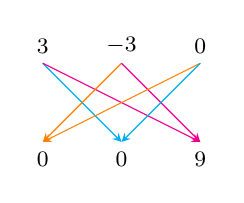
\begin{tikzpicture}[->,samples=100,>=stealth,font=\footnotesize]
                      \node[above] at (0,0) {$3$};
                      \node[above] at (1,0) {$-3$};
                      \node[above] at (2,0) {$0$};
                      \node[below] at (0,-1) {$0$};
                      \node[below] at (1,-1) {$0$};
                      \node[below] at (2,-1) {$9$};
                      \draw[cyan] (0,0)--(1,-1);
                      \draw[magenta] (0,0)--(2,-1);
                      \draw[orange] (1,0)--(0,-1);
                      \draw[magenta] (1,0)--(2,-1);
                      \draw[orange] (2,0)--(0,-1);
                      \draw[cyan] (2,0)--(1,-1);
                  \end{tikzpicture}} $\lambda_1^*=\lambda_2\lambda_3=0,~\lambda_2^*=\lambda_1\lambda_3=0,~\lambda_3^*=\lambda_1\lambda_2=-9$, 由 $\vb*{Q}^\top\vb*{AO}=\vb*{\Lambda}$ 可得
              \begin{flalign*}
                  \vb*{Q}^\top\vb*{A}^*\vb*{Q} & =\vb*{Q}^\top\qty(\vb*{Q\Lambda Q}^\top)^*\vb*{Q}=\vb*{Q}^\top\qty(\vb*{Q}^\top)^*\vb*{\Lambda}^*\vb*{Q}^*\vb*{Q}=\vb*{Q}^\top\qty|\vb*{Q}^\top|\qty(\vb*{Q}^\top)^{-1}\vb*{\Lambda}^*\qty|\vb*{Q}|\vb*{E} \\
                                               & =\vb*{Q}^\top\vb*{Q}|\vb*{Q}|\vb*{\Lambda}^*|\vb*{Q}|\vb*{E}=|\vb*{Q}|^2\vb*{\Lambda}^*\xlongequal{\det\vb*{Q}=\pm1}\vb*{\Lambda}^*
              \end{flalign*}
              因此 $\vb*{Q}^\top\qty(\vb*{A}+\vb*{A}^*)\vb*{Q}=\qty[\mqty(\dmat{3,-3,0})+\mqty(\dmat{0,0,-9})]=\mqty(\dmat{3,-3,-9})$ 即在正交变换 $\vb*{x}=\vb*{Qy}$ 下, 二次型的标准形为 $3y_1^2-3y_2^2-9y_3^2.$
        \item $\vb*{\gamma}$ 可由 $\vb*{\xi}_{1,2,3}$ 线性表示, 即 $\exists k_1,k_2,k_3$, 使得 $\vb*{\gamma}=k_1\vb*{\xi}_1+k_2\vb*{\xi}_2+k_3\vb*{\xi}_3$, 即
              $$\vb*{A}^n\vb*{\gamma}=\vb*{A}^n\qty(k_1\vb*{\xi}_1+k_2\vb*{\xi}_2+k_3\vb*{\xi}_3)=k_1\vb*{A}^n\vb*{\xi}_1+k_2\vb*{A}^n\vb*{\xi}_2+k_3\vb*{A}^n\vb*{\xi}_3=k_1\lambda_1^n\vb*{\xi}_1+k_2\lambda_2^n\vb*{\xi}_2+k_3\lambda_3^n\vb*{\xi}_3=k_1\lambda_1^n\vb*{\xi}_1+k_2\lambda_2^n\vb*{\xi}_2$$
              作增广矩阵 $\vb*{B}=\begin{pNiceArray}{ccc:c}\vb*{\xi}_1&\vb*{\xi}_2&\vb*{\xi}_3&\vb*{\gamma}\end{pNiceArray}=\begin{pNiceArray}{ccc:c}
                      1&-1&1&2\\-1&-1&1&0\\0&2&1&-1
                  \end{pNiceArray}$, 将其化为行最简形
              $$\begin{pNiceArray}{ccc:c}
                      1&-1&1&2\\-1&-1&1&0\\0&2&1&-1
                  \end{pNiceArray}\xrightarrow[\substack{r_1+r_2\\r_3-2r_2}]{\substack{r_2+r_1\\r_2\times\qty(-\frac{1}{2})}}\begin{pNiceArray}{ccc:c}
                      1&0&0&1\\0&1&-1&-1\\0&0&3&1
                  \end{pNiceArray}\xrightarrow[r_2+r_3]{r_3\times\frac{1}{3}}\begin{pNiceArray}{ccc:c}
                      1&0&0&1\\0&1&0&-\dfrac{2}{3}\\[6pt]0&0&1&\dfrac{1}{3}
                  \end{pNiceArray}$$
              因此 $k_1=1,~k_2=-\dfrac{2}{3},~k_3=\dfrac{1}{3}$, 故 $\vb*{A}^n\vb*{\gamma}=\lambda_1^n\vb*{\xi}_1-\dfrac{2}{3}\lambda_2^n\vb*{\xi}_2=\mqty(3^n+\dfrac{2}{3}\cdot(-3)^n\\[6pt]-3^n+\dfrac{2}{3}\cdot(-3)^n\\[6pt]-\dfrac{4}{3}\cdot(-3)^n).$
    \end{enumerate}
\end{solution}

\begin{example}
    设二次型 $$f(x_1,x_2,x_3)=4x_2^2-3x_3^2+2ax_1x_2-4x_1x_3+8x_2x_3~~(a\in\mathbb{N})$$
    经过正交变换 $\vb*{x}=\vb*{Qy}$ 化为标准形为 $y_1^2+6y_2^2+by_3^2$,
    \begin{enumerate}[label=(\arabic{*})]
        \item 求 $a,b$ 的值及正交变换;
        \item 证明: 二次型 $\vb*{x}^\top\qty(\vb*{A}^*+37\vb*{E})\vb*{x}$ 正定, 其中 $\vb*{A}^*$ 为 $\vb*{A}$ 的伴随矩阵.
    \end{enumerate}
\end{example}
\begin{solution}
    \begin{enumerate}[label=(\arabic{*})]
        \item 二次型的矩阵为 $\vb*{A}=\mqty(0&a&-2\\a&4&4\\-2&4&-3)$, 且 $\vb*{A}\sim\diag(1,6,b)$, 由矩阵相似可得 $\tr\vb*{A}=1+6+b,~\det\vb*{A}=6b$, 解得 $a=2,b=-6$, 因此 $\vb*{A}$ 的特征值分别为 $\lambda_1=1,~\lambda_2=6,~\lambda_3=-6$, \\
              \textbf{法一: }$|\lambda\vb*{E}-\vb*{A}|=\mqty|\lambda&-2&2\\-2&\lambda-4&-4\\2&-4&\lambda+3|$, 当 $\lambda=\lambda_1$ 时, $\qty(1\vb*{E}-\vb*{A})\vb*{x}=\vb*{0}$, 解得特征向量为 $\vb*{\xi}_1=(-2,0,1)^\top$; 当 $\lambda=\lambda_2$ 时,
              $(6\vb*{E}-\vb*{A})\vb*{x}=\vb*{0}$, 解得特征向量为 $\vb*{\xi}_2=(1,5,2)^\top$; 当 $\lambda=\lambda_3$ 时, $(-6\vb*{E}-\vb*{A})\vb*{x}=\vb*{0}$, 解得特征向量为 $\vb*{\xi}_3=(1,-1,2)^\top$, \\
              \textbf{法二: }$\lambda=\lambda_1$ 时, $1\vb*{E}-\vb*{A}=\mqty(1&-2&2\\-2&-3&-4\\2&-4&4)\xrightarrow{r_3-2r_1}\mqty(1&-2&2\\-2&-3&-4\\0&0&0)$, $r_1$ 可由 $r_2$ 与 $(3,1,6)$ 线性表示,
              则 $$(-2,-3,-4)\times(3,1,6)=(-14,0,7)\Rightarrow (-2,0,1)\Rightarrow \vb*{\xi}_1=(-2,0,1)^\top$$
              当 $\lambda=\lambda_2$ 时, $6\vb*{E}-\vb*{A}=\mqty(6&-2&2\\-2&2&-4\\2&-4&9)\xrightarrow[\substack{r_2\times\frac{3}{2}\\r_1\times\frac{1}{2}}]{\substack{r_2+\frac{1}{3}r_1\\r_3-\frac{1}{3}r_1\\\frac{3}{5}r_3+\frac{3}{2}r_2}}\mqty(3&-1&1\\0&2&-5\\0&0&0)$, $r_1$ 可由 $r_2$ 与 $(3,-3,6)$ 线性表示, 则
              $$(0,2,-5)\times(3,-3,6)=(-3,-15,-6)\Rightarrow(1,5,2)\Rightarrow \vb*{\xi}_2=(1,5,2)^\top$$
              当 $\lambda=\lambda_3$ 时, $\vb*{-6\vb*{E}-\vb*{A}}=\mqty(-6&-2&2\\-2&-10&-4\\2&-4&-3)\xrightarrow[\substack{r_2-r_1-r_3\\r_2\leftrightarrow r_3}]{\substack{r_1\times\frac{1}{2}\\r_2\times\frac{1}{2}}}\mqty(-3&-1&1\\2&-4&-3\\0&0&0)$, $r_1$ 可由 $r_2$ 与 $(-5,3,4)$ 线性表示, 则
              $$(2,-4,-3)\times(-5,3,4)=(-7,7,-14)\Rightarrow (1,-1,2)\Rightarrow \vb*{\xi}_3=(1,-1,2)^\top$$
              将特征向量 $\vb*{\xi}_{1,2,3}$ 单位化得
              $$\vb*{e}_1=\dfrac{1}{\sqrt{5}}\mqty(-2\\0\\1),~\vb*{e}_2=\dfrac{1}{\sqrt{30}}\mqty(1\\5\\2),~\vb*{e}_3=\dfrac{1}{\sqrt{6}}\mqty(1\\-1\\2)$$
              令 $\vb*{Q}=(\vb*{e}_1,\vb*{e}_2,\vb*{e}_3)$, 则 $\vb*{x}=\vb*{Qy}$ 为所求正交变换, 其中 $\vb*{Q}=\mqty(-\dfrac{2}{\sqrt{5}}&\dfrac{1}{\sqrt{30}}&\dfrac{1}{\sqrt{6}}\\[6pt]0&\dfrac{5}{\sqrt{30}}&-\dfrac{1}{\sqrt{6}}\\[6pt]\dfrac{1}{\sqrt{5}}&\dfrac{2}{\sqrt{30}}&\dfrac{2}{\sqrt{6}})$
        \item 因为 $\vb*{A}$ 的特征值分别为 $1,6,-6$, 因此 $\vb*{A}^*$ 的特征值为 $-36,-6,6$, 那么 $\vb*{A}^*+37\vb*{E}$ 的特征值为 $1,31,43$, 皆大于 0, 因此二次型 $\vb*{x}^\top\qty(\vb*{A}^*+37\vb*{E})\vb*{x}$ 正定.
    \end{enumerate}
\end{solution}

\begin{example}
    设 $\vb*{\alpha}$ 为 3 维非零实列向量, $\vb*{A}=\vb*{E}-\dfrac{a}{\vb*{\alpha}^\top\vb*{\alpha}}\vb*{\alpha\alpha}^\top$ 为正交矩阵, 其中 $a\neq0,~\vb*{E}$ 为三阶单位矩阵,
    \begin{enumerate}[label=(\arabic{*})]
        \item 求 $a$ 的值, 并证明: $\vb*{\alpha}$ 与 $\vb*{A\alpha}$ 线性相关;
        \item 当 $\vb*{\alpha}=(b,b,0)^\top~~(b\neq0)$ 时, 求正交变换 $\vb*{x}=\vb*{Qy}$ 将二次型 $f(x_1,x_2,x_3)=\vb*{x}^\top\vb*{Ax}$ 化为规范形.
    \end{enumerate}
\end{example}
\begin{solution}
    \begin{enumerate}[label=(\arabic{*})]
        \item 由 $\vb*{A}^\top=\qty(\vb*{E}-\dfrac{a}{\vb*{\alpha}^\top\vb*{\alpha}}\vb*{\alpha\alpha}^\top)^\top=\vb*{E}-\dfrac{a}{\vb*{\alpha}^\top\vb*{\alpha}}\qty(\vb*{\alpha\alpha}^\top)^\top=\vb*{E}-\dfrac{a}{\vb*{\alpha}^\top\vb*{\alpha}}\qty(\vb*{\alpha}^\top)^\top\vb*{\alpha}^\top=\vb*{E}-\dfrac{a}{\vb*{\alpha}^\top\vb*{\alpha}}\vb*{\alpha\alpha}^\top=\vb*{A}$ 可知, $\vb*{A}$ 为实对称矩阵, 那么
              \begin{flalign*}
                  \vb*{A}^2=\vb*{AA}^\top=\qty(\vb*{E}-\dfrac{a}{\vb*{\alpha}^\top\vb*{\alpha}}\vb*{\alpha\alpha}^\top)(\vb*{E}-\dfrac{a}{\vb*{\alpha}^\top\vb*{\alpha}}\vb*{\alpha\alpha}^\top)=\vb*{E}-\dfrac{2a}{\vb*{\alpha}^\top\vb*{\alpha}}\vb*{\alpha\alpha}^\top+\dfrac{a^2}{\qty(\vb*{\alpha}^\top\vb*{\alpha})^2}\vb*{\alpha}\underbrace{\vb*{\alpha}^\top\vb*{\alpha}}\vb*{\alpha}^\top=\vb*{E}+\dfrac{a^2-2a}{\vb*{\alpha}^\top\vb*{\alpha}}\vb*{\alpha\alpha}^\top
              \end{flalign*}
              又因为 $\vb*{A}$ 是正交矩阵, 所以 $\vb*{A}^2=\vb*{E}$, 即 $\dfrac{a^2-2a}{\vb*{\alpha}^\top\vb*{\alpha}}\vb*{\alpha\alpha}^\top=\vb*{O}$, 而 $\vb*{\alpha}$ 为 3 维非零实列向量, 即 $\vb*{\alpha}^\top\vb*{\alpha}\neq0,~\vb*{\alpha\alpha}^\top\neq\vb*{O}$,
              因此 $a^2-2a=0\Rightarrow a=2~~(a\neq0)$,
              $\vb*{A\alpha}=\qty(\vb*{E}-\dfrac{a}{\vb*{\alpha}^\top\vb*{\alpha}}\vb*{\alpha\alpha}^\top)\vb*{\alpha}=\vb*{\alpha}-a\vb*{\alpha}=-\vb*{\alpha}$, 因此 $\vb*{\alpha}$ 与 $\vb*{A\alpha}$ 线性相关.
        \item \textbf{法一: }当 $\vb*{\alpha}=(b,b,0)^\top~~(b\neq0)$ 时,
              $$\vb*{\alpha}^\top\vb*{\alpha}=(b,b,0)\mqty(b\\b\\0)=2b^2,~\vb*{\alpha\alpha}^\top=\mqty(b\\b\\0)(b,b,0)=\mqty(b^2&b^2&0\\b^2&b^2&0\\0&0&0)=b^2\mqty(1&1&0\\1&1&0\\0&0&0)$$
              那么 $\vb*{A}=\vb*{E}-\dfrac{2}{\vb*{\alpha}^\top\vb*{\alpha}}\vb*{\alpha\alpha}^\top=\mqty(0&-1&0\\-1&0&0\\0&0&1)$, 因此特征多项式为 (两种方法)
              \begin{enumerate}[label=(\roman{*})]
                  \item $|\lambda\vb*{E}-\vb*{A}|=\begin{pNiceArray}{cc:c}
                                \lambda&1&0\\1&\lambda&0\\ \hdottedline
                                0&0&\lambda-1
                            \end{pNiceArray}=\qty(\lambda^2-1)(\lambda-1)=0$, 得特征值为 $\lambda_1=-1,~\lambda_2=\lambda_3=1$,
                  \item $\lambda^3-\tr\vb*{A}\cdot\lambda^2+\displaystyle\sum_{1\leqslant j_1<j_2\leqslant 3}\mqty|a_{j_1j_1}&a_{j_1j_2}\\a_{j_2j_1}&a_{j_2j_2}|\cdot\lambda-\det\vb*{A}=\lambda^3-\lambda^2-\lambda+1$, 解得 $\lambda_1=-1,~\lambda_2=\lambda_3=1$,
              \end{enumerate}
              当 $\lambda=\lambda_1$ 时, 解得特征向量为 $\vb*{\xi}_1=(1,1,0)^\top$;
              当 $\lambda=\lambda_{2,3}$ 时, 解得对应的特征向量分别为 $\vb*{\xi}_2=(-1,1,0)^\top,~\vb*{\xi}_3=(0,0,1)^\top$,
              将 $\vb*{\xi}_{1,2,3}$ 分别单位化, 得
              $$\vb*{e}_1=\dfrac{1}{\sqrt{2}}\mqty(1\\1\\0),~\vb*{e}_2=\dfrac{1}{\sqrt{2}}\mqty(-1\\1\\0),~\vb*{e}_3=\mqty(0\\0\\1)$$
              令 $\vb*{Q}=(\vb*{e}_1,\vb*{e}_2,\vb*{e}_3)$, 在正交变换 $\vb*{x}=\vb*{Qy}$ 下, 标准形为 $-y_1^2+y_2^2+y_2^2$ 也是规范形.\\
              \textbf{法二: }不妨设 $\vb*{B}=\vb*{\alpha\alpha}^\top=b^2\mqty(1&1&0\\1&1&0\\0&0&0)\Rightarrow b^2\begin{pNiceMatrix}
                      \Block[borders={bottom,tikz=dashed}]{1-3}{}1 & 1 & 0 \\
                      0                                            & 0 & 0 \\
                      0                                            & 0 & 0 \\
                  \end{pNiceMatrix}$, 则 $\rank\vb*{B}=1$, 所以矩阵 $\vb*{B}$ 的特征值为
              $$\lambda_{b1}=\lambda_{b2}=0,~\lambda_{b3}=\tr\vb*{B}=\vb*{\alpha}^\top\vb*{\alpha}=2b^2$$
              又因为 $\vb*{A}=\vb*{E}-\dfrac{2}{\vb*{\alpha}^\top\vb*{\alpha}}\vb*{\alpha\alpha}^\top=\vb*{E}-\dfrac{1}{b^2}\vb*{B}$,
              因此矩阵 $\vb*{A}$ 的特征值为 $\lambda_{a1}=\lambda_{a2}=1,~\lambda_{a3}=-1$, 并且 $\lambda_{b1}$ 对应的特征向量为 $\vb*{\xi}_1=(-1,1,0)^\top$; $\lambda_{b2}$ 对应的特征向量为 $\vb*{\xi}_2=(0,0,1)^\top$;
              $$\vb*{B\alpha}=\vb*{\alpha\alpha}^\top\vb*{\alpha}=\tr\vb*{B}\cdot\vb*{\alpha}\Rightarrow\vb*{\xi}_3=(1,1,0)^\top$$
              单位化得 $\vb*{e}_1=\dfrac{1}{\sqrt{2}}\mqty(-1\\1\\0),~\vb*{e}_2=\mqty(0\\0\\1),~\vb*{e}_3=\dfrac{1}{\sqrt{2}}\mqty(1\\1\\0)$, 令 $\vb*{Q}=(\vb*{e}_1,\vb*{e}_2,\vb*{e}_3)$, 则在正交变换 $\vb*{x}=\vb*{Qy}$ 下, 标准形为 $y_1^2+y_2^2-y_3^2$  也是规范形.
    \end{enumerate}
\end{solution}

\begin{example}
    设 $\vb*{P}=\mqty(\cos\theta&-\sin\theta\\\sin\theta&\cos\theta)$ 为二阶正交矩阵, 证明: $\vb*{P}^{n}$ 可以表示为 $$\vb*{P}^{n}=\mqty(\cos(n\theta)&-\sin(n\theta)\\ \sin(n\theta)&\cos(n\theta)).$$
    \label{zjjzzmti}
\end{example}
\begin{proof}[{\songti \textbf{证}}]
    当 $n=2$ 时, $\vb*{P}^{2}=\vb*{P}\cdot\vb*{P}=\mqty(\cos\theta&-\sin\theta\\\sin\theta&\cos\theta)\mqty(\cos\theta&-\sin\theta\\\sin\theta&\cos\theta)=\mqty(\cos2\theta&-\sin2\theta\\\sin2\theta&\cos2\theta)$, 当 $n=3$ 时, $\vb*{P}^{3}=\vb*{P}^{2}\cdot\vb*{P}=\mqty(\cos2\theta&-\sin2\theta\\\sin2\theta&\cos2\theta)\mqty(\cos\theta&-\sin\theta\\\sin\theta&\cos\theta)=\mqty(\cos3\theta&-\sin3\theta\\\sin3\theta&\cos3\theta)$, 猜想 $\vb*{P}^{k}=\mqty(\cos k\theta&-\sin k\theta\\\sin k\theta&\cos k\theta)$, 下面利用数学归纳法证明:\\
    当 $k=1,2$ 时, 显然成立, 假设当 $k=n$ 时, 公式成立, 那么当 $k=n+1$ 时, 有
    \begin{flalign*}
        \vb*{P}^{n+1} & =\vb*{P}^{n}\cdot\vb*{P}=\mqty(\cos n\theta & -\sin n\theta    \\\sin n\theta&\cos n\theta)\mqty(\cos\theta&-\sin\theta\\\sin\theta&\cos\theta)=\mqty(\cos n\theta\cos\theta-\sin n\theta\sin\theta&-\cos n\theta\sin\theta-\sin n\theta\cos\theta\\ \sin n\theta\cos\theta+\cos n\theta\sin\theta&-\sin n\theta\sin\theta+\cos n\theta\cos\theta)\\
                      & =\mqty(\cos(n+1)\theta                      & -\sin(n+1)\theta \\\sin(n+1)\theta&\cos(n+1)\theta)
    \end{flalign*}
    显然此时, 猜想公式成立, 因此对一切的正整数 $n$, 猜想的公式均成立, 故 $\vb*{P}^{n}=\mqty(\cos(n\theta)&-\sin(n\theta)\\ \sin(n\theta)&\cos(n\theta)).$
\end{proof}

\begin{example}
    已知 $\vb*{A}=\mqty(1&-\dfrac{x}{n}\\ \dfrac{x}{n}&1)$, 计算 $\displaystyle \lim_{x \to 0}\qty[\lim_{n \to +\infty}\dfrac{1}{x}\qty(\vb*{E}-\vb*{A}^{n})]$ (注明: 矩阵的极限, 即它每个元素取极限, 且 $n\in\mathbb{N}^{*}$).
\end{example}
\begin{solution}
    注意到 $\vb*{A}$ 的列向量相互正交, 且模为 $|\vb*{\alpha}|=\sqrt{1^2+\qty(\pm\dfrac{x}{n})^n}=\sqrt{1+\dfrac{x^2}{n^2}}$, 把矩阵 $\vb*{A}$ 表示为 $\vb*{A}=\vb*{\alpha P}$, 其中 $\vb*{P}$ 为正交矩阵, 由例题 \ref{zjjzzmti} 知
    $$
        \vb*{A}^{n}=\vb*{\alpha}^{n}\mqty(\cos(n\theta)&-\sin(n\theta)\\ \sin(n\theta)&\cos(n\theta))
    $$
    其中 $\theta=\arcsin\qty(\dfrac{x}{n|\vb*{\alpha}|})$, 当 $n\to+\infty$ 时, 有 $$|\vb*{\alpha}|=\lim_{n \to +\infty}\qty(1+\dfrac{x^2}{n^2})^{\frac{1}{2}}=1,~|\vb*{\alpha}|^{n}=1$$
    而 $n\theta=\dfrac{x}{|\vb*{\alpha}|}\qty(\dfrac{|\vb*{\alpha}|n}{x}\arcsin\dfrac{x}{n|\vb*{\alpha}|})\to x~(n\to+\infty)$, 所以 $\displaystyle \lim_{n \to +\infty}\qty(\vb*{E}-\vb*{A}^{n})=\mqty(1-\cos x& \sin x\\ -\sin x&1-\cos x)$
    \begin{flalign*}
        \lim_{x\to0}\qty[\lim_{n \to +\infty}\dfrac{1}{x}\qty(\vb*{E}-\vb*{A}^{n})] & =\lim_{x\to0}\dfrac{1}{x}\mqty(1-\cos x & \sin x                        \\ -\sin x&1-\cos x)=\lim_{x\to0}\mqty(\dfrac{1-\cos x}{x}&\dfrac{\sin x}{x}\\ -\dfrac{\sin x}{x}&\dfrac{1-\cos x}{x})\\
                                                                                    & =\mqty(\displaystyle\lim_{x\to0}\dfrac{1-\cos x}{x}  & \displaystyle\lim_{x\to0}\dfrac{\sin x}{x} \\[6pt] \displaystyle\lim_{x\to0}-\dfrac{\sin x}{x}&\displaystyle\lim_{x\to0}\dfrac{1-\cos x}{x})=\mqty(0&1\\-1&0).
    \end{flalign*}

\end{solution}

\subsection{谱分解}

\begin{theorem}[谱分解定理]
    \label{pufjdli}若 $n$ 阶矩阵 $\vb*{A}$ 的特征值为 $\lambda_i$, 所对应特征向量为 $\vb*{x}_i$, 经过单位化和正交化, 化为两两正交的单位特征向量 $\vb*{e}_i~ (i=1,2,\cdots,n)$, 则有
    $$\vb*{A}=\sum_{i=1}^{n}\lambda_i\vb*{e}_i\vb*{e}_i^\top.$$
\end{theorem}

\begin{example}
    设 $\vb*{A}=(a_{ij})_{3\times3}$ 为实对称矩阵, $\vb*{A}$ 的每行元素之和均为 $0$, 设 $2,3$ 是 $\vb*{A}$ 的非零特征值, 则 $a_{11}$ 对应的代数余子式 $\vb*{A}_{11}$ 为
    \begin{tasks}(4)
        \task $1$
        \task $2$
        \task $5$
        \task $6$
    \end{tasks}
\end{example}
\begin{solution}
    因为 $\vb*{A}$ 的每行元素之和均为 $0$, 故由定理 \ref{hangjunhedl} 知, $\vb*{A}$ 的另一特征值为 $0$, 因此矩阵 $\vb*{A}$ 的全部特征值为 $0,2,3$, 又由定理 \ref{bsjzdtzzB} 知矩阵 $\vb*{A}$ 的伴随矩阵的特征值为
    $$\lambda_1^*=2\times3=6,~\lambda_2^*=0\times 3=0,~\lambda_3^*=0\times 2=0$$
    且 $\lambda_1^*$ 对应的特征向量为 $(1,1,1)^\top$, 又由定理 \ref{pufjdli}, 知 $$\vb*{A}^*=0+0+6=6\mqty(\dfrac{1}{\sqrt{3}}\\[6pt]\dfrac{1}{\sqrt{3}}\\[6pt]\dfrac{1}{\sqrt{3}})\qty(\dfrac{1}{\sqrt{3}}~\dfrac{1}{\sqrt{3}}~\dfrac{1}{\sqrt{3}})=\mqty(2&2&2\\2&2&2\\2&2&2)$$
    故 $\vb*{A}_{11}=2$, 选 B.
\end{solution}

\begin{example}
    设 $\vb*{A}$ 为三阶实对称不可逆矩阵, 且 $\mqty(2&-2&1\\-2&-1&2)\vb*{A}=\mqty(6&-6&3\\-12&-6&12)$, 求 $\vb*{A}.$
\end{example}
\begin{solution}
    对等式两边同时转置, 有 $\vb*{A}^\top\mqty(2&-2\\-2&-1\\1&2)=\mqty(6&-12\\-6&-6\\3&12)$, 令 $\vb*{\xi}_1=(2,-2,1)^\top,~\vb*{\xi}_2=(-2,-1,2)^\top$, 则有 $$\vb*{A}^\top\vb*{\xi}_1=3\vb*{\xi}_1,~\vb*{A}^\top\vb*{\xi}_2=6\vb*{\xi}_2\Rightarrow \lambda_1=3,~\lambda_2=6$$
    又因为 $\vb*{A}$ 不可逆, 所以 $\det\vb*{A}=0\Rightarrow \lambda_1\lambda_2\lambda_3=0\Rightarrow \lambda_3=0$, 所以 $\vb*{A}$ 的特征值分别为 $2,6,0$, 故
    $$\vb*{A}=\sum_{i=1}^{3}\lambda_i\vb*{e}_i\vb*{e}_i^\top=\sum_{i=1}^{3}\lambda_i\cdot\dfrac{\vb*{\xi}_i}{\norm*{\vb*{\xi}_i}}\cdot\qty(\dfrac{\vb*{\xi}_i}{\norm*{\vb*{\xi}_i}})^\top=3\cdot\dfrac{1}{3}\mqty(2\\-2\\1)\cdot\dfrac{1}{3}(2,-2,1)+6\cdot\dfrac{1}{3}\mqty(-2\\-1\\2)\cdot(-2,-1,2)=\mqty(4&0&-2\\0&2&-2\\-2&-2&3).$$
\end{solution}

\begin{example}
    矩阵 $\vb*{A}$ 为 3 阶实对称矩阵, 特征值为 $0,1,1$, 且 $\vb*{\alpha}_1=\mqty(1\\a\\0),~\vb*{\alpha}_2=\mqty(1\\-1\\a)$ 是 $\vb*{A}$ 的两个不同的特征向量, 若 $\vb*{A}(\vb*{\alpha}_1+\vb*{\alpha}_2)=\vb*{\alpha}_2$, 求 $\vb*{A}$.
\end{example}
\begin{solution}
    若 $\vb*{\alpha}_1,\vb*{\alpha}_2$ 都为 $0$ 的特征向量, 则 $\vb*{A}(\vb*{\alpha}_1+\vb*{\alpha}_2)=\vb*{0}$, 与已知条件矛盾;
    若 $\vb*{\alpha}_1,\vb*{\alpha}_2$ 都为 $1$ 的特征向量, 则 $\vb*{A}(\vb*{\alpha}_1+\vb*{\alpha}_2)=\vb*{\alpha}_1+\vb*{\alpha}_2$, 与已知条件矛盾;
    若 $\vb*{\alpha}_1,\vb*{\alpha}_2$ 分别为 $1,0$ 的特征向量, 则 $\vb*{A}(\vb*{\alpha}_1+\vb*{\alpha}_2)=\vb*{\alpha}_1$, 与已知条件矛盾;
    综上, $\vb*{\alpha}_1$ 与 $\vb*{\alpha}_2$ 分别为 $0,1$ 的特征向量, 又 $\vb*{A}$ 为实对称矩阵, 那么 $\vb*{\alpha}_1$ 与 $\vb*{\alpha}_2$ 相互正交, 那么它们的内积为零, 解得 $a=0$, 故
    $\vb*{\alpha}_1=(1,1,0)^\top,~\vb*{\alpha}_2=(1,-1,1)^\top$, 并且 $\vb*{A}-\vb*{E}$ 的特征值为 $-1,0,0$, 由定理 \ref{pufjdli} 知
    $$\vb*{A}-\vb*{E}=(-1)\cdot\dfrac{1}{\sqrt{2}}\mqty(1\\1\\0)\cdot\dfrac{1}{\sqrt{2}}\mqty(1,1,0)=-\dfrac{1}{2}\mqty(1&1&0\\1&1&0\\0&0&0)\Rightarrow \vb*{A}=\mqty(\dfrac{1}{2}&-\dfrac{1}{2}&0\\[6pt]-\dfrac{1}{2}&\dfrac{1}{2}&0\\[6pt]0&0&1).$$
\end{solution}

\begin{example}
    假设 3 阶实对称矩阵 $\vb*{A}$ 的秩为 2, 并且 $\vb*{AB}=\vb*{C}$, 其中 $\vb*{B}=\mqty(1&1\\0&0\\-1&1),~\vb*{C}=\mqty(-1&1\\0&0\\1&1)$, 求 $\vb*{A}$ 的所有特征值及相应的特征向量, 并求矩阵 $\vb*{A}$ 及 $\vb*{A}^{2023}.$
\end{example}
\begin{solution}
    设 $\vb*{\xi}_1=(1,0,-1)^\top,~\vb*{\xi}_2=(1,0,1)^\top$ 那么 $\vb*{B}=(\vb*{\xi}_1,\vb*{\xi}_2),~\vb*{C}=(-\vb*{\xi}_1,\vb*{\xi}_2)$, 于是 $$\vb*{AB}=\vb*{C}\Rightarrow \vb*{A}(\vb*{\xi}_1,\vb*{\xi}_2)=(-\vb*{\xi}_1,\vb*{\xi}_2)$$
    即 $\vb*{A\xi}_1=-\vb*{\xi}_1,~\vb*{A\xi}_2=\vb*{\xi}_2$, 则 $\lambda_1=-1,\lambda_2=0$ 是 $\vb*{A}$ 的特征值, $\vb*{\xi}_1,\vb*{\xi}_2$ 是 $\vb*{A}$ 的分别属于 $\lambda_1,\lambda_2$ 的特征向量, 又 $\rank\vb*{A}=2$, 则 $\vb*{\xi}_3=0$, 于是
    $$\vb*{A}=\sum_{i=1}^{3}\lambda_i\vb*{e}_1\vb*{e}_1^\top=(-1)\cdot\dfrac{1}{\sqrt{2}}\mqty(1\\0\\-1)\cdot\dfrac{1}{\sqrt{2}}(1,0,-1)+1\cdot\dfrac{1}{\sqrt{2}}\mqty(1\\0\\1)\cdot\dfrac{1}{\sqrt{2}}(1,0,1)+0=\mqty(1&0&0\\0&0&0\\0&0&1)$$
    那么 $\vb*{A}^{2023}=\vb*{A}=\mqty(1&0&0\\0&0&0\\0&0&1).$
\end{solution}

\begin{example}
    设 3 阶实对称矩阵 $\vb*{A}$ 的每行元素之和为 3, 且 $\rank\vb*{A}=1,~\vb*{\beta}=(-1,2,2)^\top$, \\
    \begin{enumerate*}[label=(\arabic{*})]
        \item 求 $\vb*{A}^n\vb*{\beta}$;
        \item 求 $\qty(\vb*{A}-\dfrac{3}{2}\vb*{E})^{2024}.$
    \end{enumerate*}
\end{example}
\begin{solution}
    \begin{enumerate}[label=(\arabic{*})]
        \item \textbf{法一: }因为 $\vb*{A}$ 的每行元素之和为 3, 故特征值 $\lambda_1=3$, 且对应的特征向量为 $\vb*{\xi}_1=(1,1,1)^\top$, 又因为 $\vb*{A}$ 是实对称矩阵, 所以 $\vb*{A}$ 一定能相似对角化, 并且由 $\rank\vb*{A}=1$, 故矩阵 $\vb*{A}$ 的非零特征值个数为 1, 即 $\lambda_2=\lambda_3=0$, 设其对应的特征向量为 $\vb*{\xi}_2,~\vb*{\xi}_3$,
              则 $\vb*{\xi}_1,\vb*{\xi}_2,\vb*{\xi}_3$ 相互正交, 故可令 $\vb*{\xi}_2=(-1,1,0)^\top,~\vb*{\xi}_3=(-1,0,1)^\top$, 因为 $\vb*{\xi}_1,\vb*{\xi}_2,\vb*{\xi}_3$ 是三维空间中线性无关的三个向量, 则其线性组合能表示该空间中的任一向量, 即 $\exists k_1,k_2,k_3$, 使得 $\vb*{\beta}=k_1\vb*{\xi}_1+k_2\vb*{\xi}_2+k_3\vb*{\xi}_3$, 即
              $$\vb*{A}^n\vb*{\beta}=\vb*{A}^n\qty(k_1\vb*{\xi}_1+k_2\vb*{\xi}_2+k_3\vb*{\xi}_3)=k_1\vb*{A}^n\vb*{\xi}_1+k_2\vb*{A}^n\vb*{\xi}_2+k_3\vb*{A}^n\vb*{\xi}_3=k_1\lambda_1^n\vb*{\xi}_1+k_2\lambda_2^n\vb*{\xi}_2+k_3\lambda_3^n\vb*{\xi}_3$$
              作增广矩阵 $\vb*{B}=\begin{pNiceArray}{ccc:c}\vb*{\xi}_1&\vb*{\xi}_2&\vb*{\xi}_3&\vb*{\beta}\end{pNiceArray}=\begin{pNiceArray}{ccc:c}1&-1&-1&-1\\1&1&0&2\\1&0&1&2\end{pNiceArray}$, 将其化为行最简形
              $$\begin{pNiceArray}{ccc:c}1&-1&-1&-1\\1&1&0&2\\1&0&1&2\end{pNiceArray}\xrightarrow[r_1+r_3]{r_2-r_1\\r_3-r_1}\begin{pNiceArray}{ccc:c}1&0&1&2\\0&1&2&3\\0&2&1&3\end{pNiceArray}\xrightarrow[\substack{r_1-r_3\\r_2-2r_3}]{\substack{r_2\leftrightarrow r_3\\r_3-2r_2\\r_3\times(-\frac{1}{3})}}\begin{pNiceArray}{ccc:c}1&0&0&2\\0&1&0&1\\0&0&1&1\end{pNiceArray}$$
              因此 $k_1=2,~k_2=1,~k_3=1$, 故 $\vb*{A}^n\vb*{\beta}=2\lambda_1^n\vb*{\xi}_1+\lambda_2^n\vb*{\xi}_2+\lambda_3^n\vb*{\xi}_3=\mqty(2\cdot 3^n\\2\cdot 3^n\\2\cdot 3^n)=3^{n}\mqty(1\\1\\1).$\\
              \textbf{法二: }同上, 得 $\lambda_1=3,~\lambda_2=\lambda_3=0,~\vb*{\xi}_1=(1,1,1)^\top$, 将 $\vb*{\xi}_1$ 单位化, 得 $\vb*{e}_1=\dfrac{1}{\sqrt{3}}\mqty(1\\1\\1)$, 因此
              $$\vb*{A}=\sum_{i=1}^{3}\lambda_i\vb*{e}_i\vb*{e}_i^\top=\lambda_1\vb*{e}_1\vb*{e}_1^\top=3\cdot\dfrac{1}{\sqrt{3}}\mqty(1\\1\\1)\cdot\dfrac{1}{\sqrt{3}}(1,1,1)=\mqty(1&1&1\\1&1&1\\1&1&1)$$
              又因为 $\rank\vb*{A}=1$, 故 $\vb*{A}^n=(\tr\vb*{A})^{n-1}\cdot\vb*{A}$, 因此 $\vb*{A}^n\vb*{\beta}=3^{n-1}\vb*{A\beta}=3^{n-1}\mqty(3\\3\\3)=3^{n}\mqty(1\\1\\1).$
        \item 因为 $\vb*{A}$ 的特征值分别为 $3,0,0$, 则 $\vb*{A}-\dfrac{3}{2}\vb*{E}$ 的特征值分别为 $\dfrac{3}{2},-\dfrac{3}{2},-\dfrac{3}{2}$, 又因为 $\vb*{A}$ 是实对称矩阵, 即 $\exists\vb*{P}$, 使得 $\vb*{P}^{-1}\vb*{AP}=\vb*{\Lambda}$, 则有
              $\vb*{P}^{-1}\qty(\vb*{A}-\dfrac{3}{2}\vb*{E})\vb*{P}=\vb*{\Lambda}_2=\mqty(\dfrac{3}{2}\\&-\dfrac{3}{2}\\&&-\dfrac{3}{2})$, 因此
              \begin{flalign*}
                  \qty(\vb*{A}-\dfrac{3}{2}\vb*{E})^{2024} & =\underbrace{\vb*{P\Lambda _2}\overbrace{\vb*{P}^{-1}\cdot \vb*{P}}^{\vb*{E}} \vb*{\Lambda _2P}^{-1}\cdots\vb*{P\Lambda _2P}^{-1}}_{2024} =\vb*{P}\vb*{\Lambda}_2^{2024}\vb*{P}^{-1}=\vb*{P}\mqty(\dfrac{3}{2} \\&-\dfrac{3}{2}\\&&-\dfrac{3}{2})^{2024}\vb*{P}^{-1}\\
                                                           & =\vb*{P}\qty(\dfrac{3}{2})^{2024}\vb*{EP}^{-1}=\qty(\dfrac{3}{2})^{2024}\vb*{PP}^{-1}=\qty(\dfrac{3}{2})^{2024}\vb*{E}.
              \end{flalign*}
    \end{enumerate}
\end{solution}

\begin{example}
    设二次型 $f(x_1,x_2,x_3)$ 的矩阵为 $\vb*{A}$, 已知 $$|\vb*{A}+\vb*{E}|=0,~\vb*{AB}-2\vb*{B}=\vb*{O}$$
    其中 $\vb*{B}=\mqty(-1&-1&-1\\1&0&2\\0&1&-1)$, 求一个正交变换 $\vb*{x}=\vb*{Qy}$, 将二次型 $f(x_1,x_2,x_3)$ 化为标准形, 并写出矩阵 $\vb*{A}$.
\end{example}
\begin{solution}
    \textbf{法一: }由 $|\vb*{A}+\vb*{E}|=|\vb*{A}-(-1)\vb*{E}|=0$, 知 $\vb*{A}$ 的一个特征值为 $\lambda_1=-1$, 且记 $\vb*{B}=(\vb*{\beta}_1,\vb*{\beta}_2,\vb*{\beta}_3)$, 由 $\vb*{AB}-2\vb*{B}=\vb*{O}$ 知
    $$\vb*{A}(\vb*{\beta}_1,\vb*{\beta}_2,\vb*{\beta}_3)=(\vb*{A\beta}_1,\vb*{A\beta}_2,\vb*{A\beta}_3)=(2\vb*{\beta}_1,2\vb*{\beta}_2,2\vb*{\beta}_3)$$
    又 $\rank\vb*{B}=2$, 所以 2 是矩阵 $\vb*{A}$ 的二重特征值, 对应的特征向量分别为\footnote{这里最好要选择矩阵 $\vb*{B}$ 中已经正交的向量, 可以由 $\vb*{B}=\mqty(0&-1&-1\\0&0&2\\0&1&-1)$, 且 $(-1,0,1)\cdot(-1,2,-1)=0$ 知选 $\vb*{\beta}_2$ 与 $\vb*{\beta}_3$ 最合适.}
    $\vb*{\xi}_2=\vb*{\beta}_2,~\vb*{\xi}_3=\vb*{\beta}_3$, 且已正交, 又因为 $\vb*{A}$ 是二次型的系数矩阵, 则 $\vb*{A}$ 是实对称矩阵\footnote{一般地, 不考虑带有虚数的多项式.}, 设 $\lambda_1$ 对应的特征向量为 $\vb*{\xi}_1$, 于是
    $$(-1,0,1)\times(-1,2,1)=(-2,-2,-2)\Rightarrow (1,1,1)\Rightarrow \vb*{\xi}_1=(1,1,1)^\top$$
    分别将特征向量 $\vb*{\xi}_{1,2,3}$ 单位化, 有 $\vb*{e}_1=\dfrac{1}{\sqrt{3}}\mqty(1\\1\\1),~\vb*{e}_2=\dfrac{1}{\sqrt{2}}\mqty(-1\\0\\1),~\vb*{e}_3=\dfrac{1}{\sqrt{6}}\mqty(-1\\2\\-1)$, 那么
    $$\vb*{Q}=(\vb*{e}_1,\vb*{e}_2,\vb*{e}_3)=\mqty(\dfrac{1}{\sqrt{3}}&-\dfrac{1}{\sqrt{2}}&-\dfrac{1}{\sqrt{6}}\\[6pt]\dfrac{1}{\sqrt{3}}&0&\dfrac{2}{\sqrt{6}}\\[6pt]\dfrac{1}{\sqrt{3}}&\dfrac{1}{\sqrt{2}}&-\dfrac{1}{\sqrt{6}})$$
    因此 $\vb*{Q}^\top\vb*{AQ}=\vb*{\Lambda}=\mqty(\dmat{-1,2,2})$, 因此二次型的标准形为 $f(y_1,y_2,y_3)=-y_1^2+2y_2^2+2y_3^2$,
    \begin{flalign*}
        \vb*{A} & =\mqty(\dfrac{1}{\sqrt{3}}  & -\dfrac{1}{\sqrt{2}} & -\dfrac{1}{\sqrt{6}} \\[6pt]\dfrac{1}{\sqrt{3}}&0&\dfrac{2}{\sqrt{6}}\\[6pt]\dfrac{1}{\sqrt{3}}&\dfrac{1}{\sqrt{2}}&-\dfrac{1}{\sqrt{6}})\mqty(\dmat{-1,2,2})\mqty(\dfrac{1}{\sqrt{3}}&-\dfrac{1}{\sqrt{2}}&-\dfrac{1}{\sqrt{6}}\\[6pt]\dfrac{1}{\sqrt{3}}&0&\dfrac{2}{\sqrt{6}}\\[6pt]\dfrac{1}{\sqrt{3}}&\dfrac{1}{\sqrt{2}}&-\dfrac{1}{\sqrt{6}})^\top\\
                & =\mqty(-\dfrac{1}{\sqrt{3}} & -\dfrac{2}{\sqrt{2}} & -\dfrac{2}{\sqrt{6}} \\[6pt]-\dfrac{1}{\sqrt{3}}&0&\dfrac{4}{\sqrt{6}}\\[6pt]-\dfrac{1}{\sqrt{3}}&\dfrac{2}{\sqrt{2}}&-\dfrac{2}{\sqrt{6}})\mqty(\dfrac{1}{\sqrt{3}}&-\dfrac{1}{\sqrt{2}}&-\dfrac{1}{\sqrt{6}}\\[6pt]\dfrac{1}{\sqrt{3}}&0&\dfrac{2}{\sqrt{6}}\\[6pt]\dfrac{1}{\sqrt{3}}&\dfrac{1}{\sqrt{2}}&-\dfrac{1}{\sqrt{6}})^\top=\mqty(1&-1&-1\\-1&1&-1\\-1&-1&1).
    \end{flalign*}
    \textbf{法二: }同上得 $\lambda_1=-1,~\lambda_2=\lambda_3=2,~\vb*{\xi}_1=(1,1,1)^\top,~\vb*{\xi}_2=(-1,0,1)^\top,~\vb*{\xi}_3=(-1,2,-1)^\top$, 那么 $\vb*{A}-2\vb*{E}$ 的特征值分别为 $-3,0,0$, 则
    $$\vb*{A}-2\vb*{E}=-3\vb*{e}_1\vb*{e}_1^\top=-3\cdot\dfrac{1}{\sqrt{3}}\mqty(1\\1\\1)\cdot\dfrac{1}{\sqrt{3}}(1,1,1)=-\mqty(1&1&1\\1&1&1\\1&1&1)\Rightarrow \vb*{A}=\mqty(1&-1&-1\\-1&1&-1\\-1&-1&1).$$
\end{solution}

\begin{example}
    设 3 阶实矩阵 $\vb*{A}$ 及其伴随矩阵 $\vb*{A}^*$ 满足 $\vb*{A}-\vb*{A}^*-\vb*{E}=\vb*{O}$, 且 $\det\vb*{A}=2$,
    \begin{enumerate}[label=(\arabic{*})]
        \item 证明: $\vb*{A}$ 能相似对角化;
        \item 如果 $\vb*{A}$ 为实对称矩阵, 且 $\vb*{\xi}=(1,1,-1)^\top$ 是齐次线性方程组 $(\vb*{A}-2\vb*{E})\vb*{x}=\vb*{0}$ 的一个解, 求对称矩阵 $\vb*{B}$, 使得 $\vb*{B}^2=\vb*{A}+\vb*{E}$.
    \end{enumerate}
\end{example}
\begin{solution}
    \begin{enumerate}[label=(\arabic{*})]
        \item 因为 $\vb*{AA}^*=\vb*{A}^*\vb*{A}=|\vb*{A}|\vb*{E}=2\vb*{E}$, 所以
              $$\vb*{A}\qty(\vb*{A}-\vb*{A}^*-\vb*{E})=\vb*{O}\Rightarrow \vb*{A}^2-\vb*{A}-2\vb*{E}=\vb*{O}\Rightarrow (\vb*{A}+\vb*{E})(\vb*{A}-2\vb*{E})=\vb*{O}$$
              那么 $$3=\rank\qty[(\vb*{A}+\vb*{E})-(\vb*{A}-2\vb*{E})]\leqslant \rank(\vb*{A}+\vb*{E})+\rank(\vb*{A}-2\vb*{E})\leqslant 3\Rightarrow \rank(\vb*{A}+\vb*{E})+\rank(\vb*{A}-2\vb*{E})=3$$
              又因为属于特征值 -1 的特征向量的个数为 $3-\rank(\vb*{A}+\vb*{E})$, 属于特征值 2 的特征向量的个数为 $3-\rank(\vb*{A}-2\vb*{E})$, 相加得 $\vb*{A}$ 有 3 个线性无关的特征向量, 即 $\vb*{A}$ 能相似对角化.
        \item 由 (1) 可知, 矩阵 $\vb*{A}$ 的两个特征值分别为 $\lambda_1=-1,~\lambda_2=2$, 且 $\det\vb*{A}=2=\lambda_1\lambda_2\lambda_3$, 所以 $\lambda_3=-1$, 又因为 $\vb*{\xi}=(1,1,-1)^\top$ 是齐次线性方程组 $(\vb*{A}-2\vb*{E})\vb*{x}=\vb*{0}$ 的一个解,
              所以 $\lambda_2$ 对应的特征向量为 $\vb*{\xi}=(1,1,-1)^\top$, 故 $\vb*{A}+\vb*{E}$ 的两个特征值分别为 $3,~0,~0$, 所以存在正交矩阵 $\vb*{Q}$, 使得 $\vb*{Q}^\top(\vb*{A}+\vb*{E})\vb*{Q}=\diag(3,0,0)$
              因此 $$\vb*{A}+\vb*{E}=\vb*{Q}\diag(3,0,0)\vb*{Q}^\top=\vb*{Q}\mqty(\dmat{\pm\sqrt{3},0,0})\vb*{Q}^\top\vb*{Q}\mqty(\dmat{\pm\sqrt{3},0,0})\vb*{Q}^\top\Rightarrow \vb*{B}=\vb*{Q}\mqty(\dmat{\pm\sqrt{3},0,0})\vb*{Q}^\top$$
              即 $\vb*{B}=\pm\sqrt{3}\cdot\dfrac{1}{\sqrt{3}}\mqty(1\\1\\-1)\cdot\dfrac{1}{\sqrt{3}}(1,1,-1)=\pm\dfrac{\sqrt{3}}{3}\mqty(1&1&-1\\1&1&-1\\-1&-1&1).$
    \end{enumerate}
\end{solution}

\begin{example}
    设 $\vb*{A}=(a_{ij})$ 为三阶实对称矩阵, $\det\vb*{A}=-2,~\tr\vb*{A}=0$, 记 $$f(x_1,x_2,x_3,x_4)=\mqty|x_1^2&x_2&x_3&x_4\\x_2&a_{11}&a_{12}&a_{13}\\x_3&a_{21}&a_{22}&a_{23}\\x_4&a_{31}&a_{32}&a_{33}|$$
    已知 $(1,1,1)^\top$ 为线性方程组 $\qty(\vb*{A}^*-\vb*{E})\vb*{x}=\vb*{0}$ 的解, 其中 $\vb*{A}^*$ 为 $\vb*{A}$ 的伴随矩阵, 试给出正交变换 $\vb*{x}=\vb*{Qy}$, 使得 $f(x_1,x_2,x_3,x_4)$ 化为标准形, 并求出矩阵 $\vb*{A}.$
\end{example}
\begin{solution}
    记 $\vb*{x}=(x_2,x_3,x_4)^\top$, 由行列式的降阶公式 $\mqty|\vb*{A}&\vb*{B}\\\vb*{C}&\vb*{D}|=|\vb*{D}|~\qty|\vb*{A}-\vb*{BD}^{-1}\vb*{C}|$, 得
    $$f=\mqty|x_1^2&\vb*{x}^\top\\\vb*{x}&\vb*{A}|=\det\vb*{A}\cdot\qty(x_1^2-\vb*{x}^\top\vb*{A}^{-1}\vb*{x})=-2x_1^2-\vb*{x}^\top\vb*{A}^*\vb*{x}$$
    问题归结为求正交变换 $\vb*{x}=\vb*{Py}$ 使得 $g(\vb*{x})=\vb*{x}^\top\vb*{A}^*\vb*{x}$ 化为标准形, 令 $\vb*{\alpha}_1=(1,1,1)^\top$, 那么
    $$\vb*{A}^*\vb*{\alpha}_1=\vb*{\alpha}_1\Rightarrow \vb*{AA}^*\vb*{\alpha}_1=\vb*{A\alpha}_1\Rightarrow \vb*{A\alpha}_1=\det\vb*{A}\cdot\vb*{E\alpha}_1=-2\vb*{\alpha_1}$$
    即 $\lambda_1=-2$ 是矩阵 $\vb*{A}$ 的一个特征值, 其对应的特征向量为 $\vb*{\alpha}_1=(1,1,1)^\top$, 又因为 $\det\vb*{A}=-2,~\tr\vb*{A}=0$, 所以 $\begin{cases}
            \lambda_1\cdot\lambda_2\cdot\lambda_3=-2 \\
            \lambda_1+\lambda_2+\lambda_3=0
        \end{cases}$ 解得 $\lambda_2=\lambda_3=1$, 设 $\lambda_2$ 对应的特征向量为 $(t_1,t_2,t_3)^\top$, 因为 $\vb*{A}$ 是三阶实对称矩阵, 所以不同特征值的特征向量是正交的, 所以 $t_1+t_2+t_3=0$, 由此解得 $\vb*{A}$ 的属于 1 的两个相互正交的特征向量为 $\vb*{\alpha}_2=(-1,1,0)^\top,~\vb*{\alpha}_3=(-1,-1,2)^\top$, 取正交矩阵
    $$\vb*{P}=\qty(\dfrac{\vb*{\alpha}_1}{\norm*{\vb*{\alpha}_1}},\dfrac{\vb*{\alpha}_2}{\norm*{\vb*{\alpha}_2}},\dfrac{\vb*{\alpha}_3}{\norm*{\vb*{\alpha}_3}})=\mqty(\dfrac{1}{\sqrt{3}}&-\dfrac{1}{\sqrt{2}}&-\dfrac{1}{\sqrt{6}}\\[6pt]\dfrac{1}{\sqrt{3}}&\dfrac{1}{\sqrt{2}}&-\dfrac{1}{\sqrt{6}}\\[6pt]\dfrac{1}{\sqrt{3}}&0&\dfrac{2}{\sqrt{6}})$$
    则 $\vb*{P}^\top\vb*{AP}=\diag(-2,1,1)$, 因此 $\vb*{P}^\top\vb*{A}^*\vb*{P}=|\vb*{A}|\qty(\vb*{P}^\top\vb*{AP})^{-1}\diag(1,-2,-2)$, 于是, 可取正交变换 $\vb*{x}=\vb*{Py}$, 其中 $\vb*{y}=(y_2,y_3,y_4)^\top$, 使得 $g=\vb*{y}^\top\qty(\vb*{P}^\top\vb*{A}^*\vb*{P})\vb*{y}=y_2^2-2y_3^2-2y_4^2$,
    最后再令 $x_1=y_1$, 以及 $\vb*{Q}=\mqty(1\\&\vb*{P})$, 则正交变换 $\mqty(x_1\\\vb*{x})=\vb*{Q}\mqty(y_1\\\vb*{y})$ 可使 $f$ 化为标准形 $f=-2y_1^2-y_2^2+2y_3^2+2y_4^2$, 并且由
    $$\vb*{A}-\vb*{E}=\sum_{i=1}^{3}\lambda_i\vb*{e}_i\vb*{e}_i^\top=-3\cdot\dfrac{1}{\sqrt{3}}\mqty(1\\1\\1)\cdot\dfrac{1}{\sqrt{3}}(1,1,1)=-\mqty(1&1&1\\1&1&1\\1&1&1)\Rightarrow \vb*{A}=\vb*{E}-\mqty(1&1&1\\1&1&1\\1&1&1)=\mqty(0&-1&-1\\-1&0&-1\\-1&-1&0)$$
    其中 $\vb*{e}_i=\dfrac{\vb*{\alpha}_i}{\norm*{\vb*{\alpha}_i}}$.
\end{solution}

\subsection{正交变换的应用}

\subsubsection{几何应用}

\begin{example}
    设中心在原点的椭圆方程为 $x^2-4xy+5y^2=1$, 求该椭圆的长半轴与短半轴.
\end{example}
\begin{solution}
    方程系数矩阵为 $\vb*{A}=\mqty(1&-2\\-2&5)$, 那么 $|\lambda\vb*{E}-\vb*{A}|=\mqty|\lambda-1 & 2\\2&\lambda-5|=0\Rightarrow \lambda_{1,2}=3\pm 2\sqrt{2}$, 即
    $$\qty(3+2\sqrt{2})z_1^2+\qty(3-2\sqrt{2})z_2^2=1\Rightarrow \dfrac{z_1^2}{\dfrac{1}{3+2\sqrt{2}}}+\dfrac{z_2^2}{\dfrac{1}{3-2\sqrt{2}}}=1\Rightarrow \dfrac{z_1^2}{\qty(\dfrac{1-\sqrt{2}}{1})^2}+\dfrac{z_2^2}{\qty(\dfrac{1+\sqrt{2}}{1})^2}=1$$
    因此, 长半轴长度为 $\sqrt{2}+1$, 短半轴长度为 $\sqrt{2}-1.$
\end{solution}

\begin{example}
    求椭圆 $2x^2+4xy+5y^2=1$ 的面积.
\end{example}
\begin{solution}
    由题意 $f=\vb*{X}^\top\vb*{AX}=\vb*{X}^\top\mqty(2&2\\2&5)\vb*{X}=1$, 那么 $|\lambda \vb*{E}-\vb*{A}|=(\lambda-6)(\lambda-1)=0\Rightarrow \lambda_1=6,\lambda_2=1$, 因此
    $$(\lambda_i\vb*{E}-\vb*{A})\vb*{\alpha}_i=\vb*{0}\Rightarrow \vb*{\alpha}_1=(1,2)^\top,\vb*{\alpha}_2=(-2,1)^\top\Rightarrow Q=\qty(\dfrac{\vb*{\alpha}_1}{|\vb*{\alpha}_1|},\dfrac{\vb*{\alpha}_2}{|\vb*{\alpha}_2|})$$
    $f=\vb*{X}^\top\vb*{AX}$ 在 $\vb*{X}=\vb*{QY}$ 的作用下, 化为 $f=\vb*{Y}^\top\vb*{Q}^\top\vb*{AQY}=6y_1^2+y_2^2=1\Rightarrow S=\dfrac{\pi}{\sqrt{6}}.$
\end{solution}

\begin{inference}[一般椭圆面积公式]
    设曲线 $Ax^2+2Bxy+Cy^2=1,A>0$, 且 $AC-B^2>0$, 那么该曲线为椭圆, 该椭圆的面积 $S=\dfrac{\pi}{\sqrt{AC-B^2}}.$
\end{inference}

\subsubsection{二次型与曲面方程}

% \begin{example}[2016 数一]
%     设二次型 $f(x_1,x_2,x_3)=x_1^2+x_2^2+x_3^3+4x_1x_2+4x_1x_3+4x_2x_3$, 则 $f=2$, 在空间直角坐标系下表示的二次曲面为
%     \begin{tasks}(4)
%         \task 单叶双曲面
%         \task 双叶双曲面
%         \task 椭球面
%         \task 柱面
%     \end{tasks}
% \end{example}

\begin{example}
    转换一般二次型方程 $$2x^2+5y^2+5z^2+4xy-4xz-8yz=1$$
    为标准二次型, 并判定其在直角坐标系 $O-xyz$ 中描述的图形类型.
\end{example}
\begin{solution}
    因为 $\begin{NiceArray}{c:ccc}
              & x  & y  & z  \\ \hdottedline
            x & 2  & 2  & -2 \\
            y & 2  & 5  & -4 \\
            z & -2 & -4 & 5
        \end{NiceArray}$, 所以二次型对应的矩阵为 $\vb*{A}=\begin{pmatrix}
            2  & 2  & -2 \\
            2  & 5  & -4 \\
            -2 & -4 & 5
        \end{pmatrix}$, 故特征多项式为
    $$|\lambda\vb*{E}-\vb*{A}|=\begin{vmatrix}
            \lambda -2 & -2         & 2         \\
            -2         & \lambda -5 & 4         \\
            2          & 4          & \lambda-5
        \end{vmatrix}\xlongequal[r_3+2r_1]{r_2+r_3}\begin{vmatrix}
            \lambda -2  & -2         & 2          \\
            0           & \lambda -1 & \lambda -1 \\
            2\lambda -2 & 0          & \lambda -1
        \end{vmatrix}=(\lambda-1)^2(\lambda-10)=0$$
    得矩阵 $\vb*{A}$ 的特征值 $\lambda_{1,2,3}=1,1,10$, 对 $\lambda=1$, 解齐次方程组
    $$\left\{\begin{matrix}
            -x  & - & 2y & + & 2z & =0 \\
            -2x & - & 4y & + & 4z & =0 \\
            2x  & + & 4y & - & 4z & =0
        \end{matrix}\right.$$
    得基础解系 $\vb*{\alpha}_1=(2,-1,0)^\top$ 与 $\vb*{\alpha}_2=(2,0,1)^\top$, 将他们正交化, 得 $\vb*{\beta}_1=\vb*{\alpha}_1,~\vb*{\beta}_2=\vb*{\alpha}_2-\dfrac{\comm{\vb*{\alpha}_2}{\vb*{\beta}_1}}{\norm{\vb*{\beta}_1}^2}\vb*{\beta}_1$, 即
    $$\vb*{\beta}_1=(2,-1,0)^\top,~\vb*{\beta}_2=(2,0,1)^\top-\dfrac{4}{5}(2,-1,0)^\top=\qty(\dfrac{2}{5},\dfrac{4}{5},1)^\top$$
    单位化: $\vb*{e}_1=\qty(\dfrac{2}{\sqrt{5}},-\dfrac{1}{\sqrt{5}},0)^\top,~\vb*{e}_2=\qty(\dfrac{2\sqrt{5}}{15},\dfrac{4\sqrt{5}}{15},\dfrac{\sqrt{5}}{3})^\top$; 对 $\lambda=10$, 解齐次方程组
    $$\left\{\begin{matrix}
            8x  & - & 2y & + & 2z & =0 \\
            -2x & + & 5y & + & 4z & =0 \\
            2x  & + & 4y & + & 5z & =0
        \end{matrix}\right.$$ 得基础解系 $(1,2,-2)^\top$, 单位化得 $\vb*{e}_3=\qty(\dfrac{1}{3},\dfrac{2}{3},-\dfrac{2}{3})^\top$, 令 $\vb*{T}=\begin{pmatrix}
            \dfrac{2\sqrt{5} }{5} & \dfrac{2\sqrt{5}}{15} & \dfrac{1}{3}  \\[6pt]
            -\dfrac{\sqrt5}{5}    & \dfrac{4\sqrt{5}}{15} & \dfrac{2}{3}  \\[6pt]
            0                     & \dfrac{\sqrt5}{2}     & -\dfrac{2}{3}
        \end{pmatrix}$, 则有正交变换 $\vb*{y}=\vb*{Tx}$, 即 $\left\{\begin{matrix}
            x= & \dfrac{2\sqrt{5} }{5} u & + & \dfrac{2\sqrt{5}}{15}v & + & \dfrac{1}{3}w  \\[6pt]
            y= & -\dfrac{\sqrt5}{5}u     & + & \dfrac{4\sqrt{5}}{15}v & + & \dfrac{2}{3}w  \\[6pt]
            z= &                         &   & \dfrac{\sqrt5}{2}  v   & - & \dfrac{2}{3} w
        \end{matrix}\right.$, 将原二次型化为 $u^2+v^2+10w^2=1$, 即为椭球面.
\end{solution}

\begin{example}
    用正交变换将二次曲面的方程 $$x^2-2y^2-2z^2-4xy+4xz+8yz-27=0$$ 化为标准方程, 并说明该曲面是什么曲面.
\end{example}
\begin{solution}
    设 $\vb*{A}=\mqty(1&-2&2\\-2&-2&4\\2&4&-2),~\vb*{X}=(x,y,z)^\top$, 则曲面方程为 $\vb*{X}^\top\vb*{AX}=27$, $\vb*{A}$ 的特征多项式为
    $$|\lambda\vb*{E}-\vb*{A}|=\mqty|\lambda-1&2&-2\\2&\lambda+2&-4\\-2&-4&\lambda+2|=(\lambda-2)^2(\lambda+7)=0$$
    对于 $\lambda_{1,2}=2$, 解齐次线性方程组 $(\lambda_{1,2}\vb*{E}-\vb*{A})\vb*{X}=\vb*{0}$, 求得对应的线性无关的特征向量为 $\vb*{\alpha}_1=(-2,1,0)^\top,~\vb*{\alpha}_2=(2,0,1)^\top$, 并将其正交化, 得
    $$\vb*{e}_1=\dfrac{1}{\sqrt{5}}(-2,1,0)^\top,~\vb*{e}_2=\dfrac{1}{3\sqrt{5}}(2,4,5)^\top$$
    对于 $\lambda_3=-7$, 解齐次线性方程组 $(\lambda_3\vb*{E}-\vb*{A})\vb*{X}=\vb*{0}$, 求得对应的单位化特征向量为 $\vb*{e}_3=\dfrac{1}{3}(1,2,-2)^\top$,
    取正交矩阵 $\vb*{Q}=(\vb*{e}_1,\vb*{e}_2,\vb*{e}_3)$, 令 $\vb*{X}'=(x',y',z')^\top$, 则正交变换 $\vb*{X}=\vb*{QX}'$ 将曲面的方程 $\vb*{X}^\top\vb*{AX}=27$ 可化为如下标准方程
    $$2x'^2+2y'^2-7z'^2=27$$ 这是单叶双曲面.
\end{solution}

\subsubsection{最值问题}

\begin{example}
    已知二次型 $f(x_1,x_2,x_3)=x_1^2-3x_2^2-3x_3^2+2x_1x_2-4x_1x_3$,
    \begin{enumerate}[label=(\arabic{*})]
        \item 写出二次型 $f$ 的矩阵表达式;
        \item 用正交变换把二次型 $f$ 化为标准形, 并写出相应的正交矩阵;
        \item 若 $\vb*{x}^\top\vb*{x}=5$, 求 $f_{max}.$
    \end{enumerate}
\end{example}
\begin{solution}
    \begin{enumerate}[label=(\arabic{*})]
        \item $f(x_1,x_2,x_3)=\vb*{x}^\top\vb*{Ax}=(x_1,x_2,x_3)\mqty(1&1&-2\\1&-3&0\\-2&0&-3)\mqty(x_1\\x_2\\x_3)$.
        \item $|\lambda\vb*{E}-\vb*{A}|=\mqty|\lambda-1&-1&2\\-1&\lambda+3&0\\2&0&\lambda+3|=(\lambda-2)(\lambda+3)(\lambda+4)$, 当 $\lambda=2$ 时, 由 $(2\vb*{E}-\vb*{A})\vb*{x}=\vb*{O}$, 即
              $$2\vb*{E}-\vb*{A}=\mqty(1&-1&2\\-1&5&0\\2&0&5)\xrightarrow[r_3-2r_1]{r_2+r_1}\mqty(1&-1&2\\0&4&2\\0&2&1)\xrightarrow[r_2\times\frac{1}{2}]{r_3-\frac{1}{2}r_2}\mqty(1&-1&2\\0&2&1\\0&0&0)\xrightarrow{r_1-2r_2}\mqty(1&-5&0\\0&2&1\\0&0&0)$$
              则基础解系 $\vb*{\alpha}_1=(5,1,-2)^\top$; 当 $\lambda=-3$ 时, $(-3\vb*{E}-\vb*{A})\vb*{x}=\vb*{O}$, 即
              $$-3\vb*{E}-\vb*{A}=\mqty(-4&-1&2\\-1&0&0\\2&0&0)\xrightarrow[\substack{r_2+4r_1\\r_3-2r_1}]{\substack{r_2\times(-1)\\r_1\leftrightarrow r_2}}\mqty(1&0&0\\0&-1&2\\0&0&0)$$
              则基础解系 $\vb*{\alpha}_2=(0,2,1)^\top$; 当 $\lambda=-4$ 时, $(-4\vb*{E}-\vb*{A})\vb*{x}=\vb*{O}$, 即
              $$-4\vb*{E}-\vb*{A}=\mqty(-5&-1&2\\-1&-1&0\\2&0&-1)\xrightarrow[\substack{r_2+5r_1\\r_3-2r_1}]{\substack{r_2\times(-1)\\r_1\leftrightarrow r_2}}\mqty(1&1&0\\0&4&2\\0&-2&-1)\xrightarrow[r_2\times\frac{1}{2}]{r_3+\frac{1}{2}r_2}\mqty(1&1&0\\0&4&2\\0&0&0)$$
              则基础解系 $\vb*{\alpha}_3=(-1,1,-2)$, 因为 $\vb*{A}$ 为实对称矩阵, 对应于不同特征值的特征向量相互正交, 即 $\vb*{\alpha}_1,\vb*{\alpha}_2,\vb*{\alpha}_3$ 相互正交, 故只需将其单位化, 有
              $$\vb*{e}_1=\dfrac{1}{\sqrt{30}}\mqty(5\\1\\-2),~\vb*{e}_2=\dfrac{1}{\sqrt{5}}\mqty(0\\2\\1),~\vb*{e}_3=\dfrac{1}{\sqrt{6}}\mqty(-1\\1\\-2)$$
              令 $\vb*{Q}=\mqty(\vb*{e}_1,\vb*{e}_2,\vb*{e}_3)=\mqty(\dfrac{5}{\sqrt{30}}&0&-\dfrac{1}{\sqrt{6}}\\[6pt]
                  \dfrac{1}{\sqrt{30}}&\dfrac{2}{\sqrt{5}}&\dfrac{1}{\sqrt{6}}\\[6pt]
                  -\dfrac{2}{\sqrt{30}} & \dfrac{1}{\sqrt{5}} & -\dfrac{2}{\sqrt{6}}
                  )$ 则经正交变换 $\vb*{x}=\vb*{Qy}$, 二次型化为标准形 $$f(x_1,x_2,x_3)=\vb*{x}^\top\vb*{Ax}=(\vb*{Qy})^\top\vb*{A}(\vb*{Qy})=\vb*{y}^\top\vb*{Q}^\top\vb*{AQy}=\vb*{y}^\top\vb*{\Lambda y}=2y_1^2-3y_2^2-4y_3^2.$$
        \item 因为 $\vb*{x}^\top\vb*{x}=(\vb*{Qy})^\top(\vb*{Qy})=\vb*{y}^\top\vb*{Q}^\top\vb*{Qy}=\vb*{y}^\top\vb*{y}=5$, 故求 $f$ 在 $\vb*{y}^\top\vb*{y}=5$ 的最大值, 则由定理 \ref{tzzbds} 得
              $$f(x_1,x_2,x_3)=\vb*{x}^\top\vb*{Ax}=\vb*{y}^\top\vb*{\Lambda y}=2y_1^2-3y_2^2-4y_3^2\leqslant 2\qty(y_1^2+y_2^2+y_3^2)=10$$
    \end{enumerate}
\end{solution}

\begin{example}
    已知二次型 $f(x,y,z)=3x^2+2y^2+2z^2+2xy+2zx$,
    \begin{enumerate}[label=(\arabic{*})]
        \item 用正交变换把二次型 $f$ 化为标准形, 并写出相应的正交矩阵;
        \item 求函数 $f(x,y,z)$ 在单位球面 $x^2+y^2+z^2=1$ 上的最大值与最小值.
    \end{enumerate}
\end{example}
\begin{solution}
    \begin{enumerate}[label=(\arabic{*})]
        \item 二次型对应的矩阵 $\vb*{A}=\mqty(3&1&1\\1&2&0\\1&0&2)$, 则特征多项式为
              $$f(\lambda)=\lambda^3-7\lambda^2+14\lambda-8=(\lambda-1)(\lambda-2)(\lambda-4)\Rightarrow \lambda_1=1,~\lambda_2=2,~\lambda_3=4$$
              那么 $\lambda_1\vb*{E}-\vb*{A}=\mqty(-2&-1&-1\\-1&-1&0\\-1&0&-1)\to\mqty(1&1&0\\1&0&1\\0&0&0)$ 其中 $r_1$ 可由 $r_2$ 与 $(0,1,-1)$ 线性表示, 则 $$(1,0,1)\times(0,1,-1)=(-1,1,1)\Rightarrow \vb*{\xi}_1=(-1,1,1)^\top$$
              同理可得 $\vb*{\xi}_2=(0,-1,1)^\top,~\vb*{\xi}_3=(2,1,1)^\top$, 则令 $\vb*{P}=\qty(\dfrac{\vb*{\xi}_1}{\norm*{\vb*{\xi}_1}},\dfrac{\vb*{\xi}_2}{\norm*{\vb*{\xi}_2}},\dfrac{\vb*{\xi}_3}{\norm*{\vb*{\xi}_3}})=\mqty(-\dfrac{1}{\sqrt{3}}&0&\dfrac{2}{\sqrt{6}}\\[6pt]\dfrac{1}{\sqrt{3}}&-\dfrac{1}{\sqrt{2}}&\dfrac{1}{\sqrt{6}}\\[6pt]\dfrac{1}{\sqrt{3}}&\dfrac{1}{\sqrt{2}}&\dfrac{1}{\sqrt{6}})$,
              于是正交变换 $\vb*{X}'=\vb*{P}^\top\vb*{X}$, 其中 $\vb*{X}'=(x',y',z'),~\vb*{X}=(x,y,z).$
        \item 注意到
              $$x^2+y^2+z^2=\vb*{X}^\top\vb*{X}=\vb*{X}^\top\vb*{PP}^\top\vb*{X}=\qty(\vb*{P}^\top\vb*{X})^\top\qty(\vb*{P}^\top\vb*{X})=\vb*{X}'^\top\vb*{X}'=x'^2+y'^2+z'^2$$
              $$f(x,y,z)=\vb*{X}^\top\vb*{AX}=\vb*{X}^\top\vb*{P\Lambda P}^\top\vb*{X}=\qty(\vb*{P}^\top\vb*{X})\vb*{\Lambda}\qty(\vb*{P}^\top\vb*{X})=\qty(\vb*{X}')^\top\vb*{\Lambda}\qty(\vb*{X}')=x'^2+2y'^2+4z'^2$$
              函数 $f(x,y,z)$ 在单位球面 $x^2+y^2+z^2=1$ 上的最大值与最小值也就是函数 $x'^2+2y'^2+4z'^2$ 在 $x'^2+y'^2+z'^2=1$ 上的最大值与最小值, 因此
              \begin{flalign*}
                  f_{max} & =\max_{x'^2+y'^2+z'^2=1}\qty{x'^2+2y'^2+4z'^2}=\max_{x'^2+y'^2+z'^2=1}\qty{4-3x'^2-2y'^2}=\eval{4-3x'^2-2y'^2}_{(0,0,1)}=4 \\
                  f_{min} & =\min_{x'^2+y'^2+z'^2=1}\qty{x'^2+2y'^2+4z'^2}=\min_{x'^2+y'^2+z'^2=1}\qty{1+y'^2+3z'^2}=\eval{1+y'^2+3z'^2}_{(1,0,0)}=1.
              \end{flalign*}
    \end{enumerate}
\end{solution}

\subsection{直角坐标变换}

设一般二次曲面的方程为
$$a_{11}x^2+a_{22}y^2+a_{33}z^2+2a_{12}xy+2a_{13}xz+2a_{23}yz+2b_1x+2b_2y+2b_3z+c=0$$
写出矩阵形式为
\begin{equation*}
    \vb*{x}^\top\vb*{Ax}+2\vb*{B}^\top\vb*{x}+c=0
    \tag{1}
\end{equation*}
其中 $\vb*{A}=\mqty(\xmat*{a}{3}{3})~~(a_{ij}=a_{ji}),~\vb*{x}=(x,y,z)^\top,~\vb*{B}=(b_1,b_2,b_3)^\top$,
作正交矩阵 $\vb*{Q}$, 使 $\vb*{Q}^\top\vb*{AQ}=\diag(\lambda_1,\lambda_2,\lambda_3)$, 其中 $\lambda_{1,2,3}$ 为 $\vb*{A}$ 的特征值, 那么化为标准方程可分为两种情况进行.
\begin{enumerate}[label=(\arabic{*})]
    \item 若方程组 $\vb*{Ax}+\vb*{B}=\vb*{0}$ 有解, 则取其任意一个解 $\vb*{\delta}$, 作直角坐标变换 $$\vb*{x}=\vb*{Qx}'+\vb*{\delta}$$ 代入 (1) 式得
          $$\vb*{x}'^\top\vb*{Q}^\top\vb*{AQx}'+2(\vb*{A\delta}+\vb*{B})^\top\vb*{Qx}'+\vb*{\delta}^\top\vb*{A\delta}+2\vb*{B}^\top\vb*{\delta}+c=0$$
          由 $\vb*{Q}^\top\vb*{AQ}=\diag(\lambda_1,\lambda_2,\lambda_3),~\vb*{A\delta}+\vb*{B}=\vb*{0}$, 可得
          \begin{equation*}
              \lambda_1 x'^2+\lambda_2 y'^2+\lambda_3 z'^2=d
              \tag{2}
          \end{equation*}
          其中 $d=-\qty(\vb*{\delta}^\top\vb*{A\delta}+2\vb*{B}^\top\vb*{\delta}+c)$, (2) 式就是 (1) 式的标准方程.
    \item 若方程组 $\vb*{Ax}+\vb*{B}=0$ 无解, 则必有 $\det\vb*{A}=0$, 由于 $\det\vb*{A}=\lambda_1\lambda_2\lambda_3$, 则 $\lambda_1,\lambda_2,\lambda_3$ 中至少有一个为 0, 不妨设 $\lambda_1\neq 0,\lambda_3=0$, 作正交变换 $\vb*{x}=\vb*{Qx}'$, 代入 (1) 式得
          \begin{equation*}
              \lambda_1x'^2+\lambda_2y'^2+2b'_1x'+2b'_2y'+2b'_3z'+c=0
              \tag{3}
          \end{equation*}
          \begin{enumerate}[label=(\roman{*})]
              \item 若 $\lambda_2\neq0$, 将 (3) 配方得
                    \begin{equation*}
                        \lambda_1\qty(x'+b_1')^2+\lambda_2\qty(y'+b_2')^2=d-2b_3'z'
                        \tag{4}
                    \end{equation*}
                    其中 $d=\lambda_1b_1'^2+\lambda_2b_2'^2-c$, 当 $b_3'\neq0$ 时, 作平移 $$\begin{cases}
                            x''=x'+b_1' \\
                            y''=y'+b_2' \\
                            z''=z'-\dfrac{d}{2b_3'}
                        \end{cases}$$ 则 (4) 式化为标准方程 $$\lambda_1x''^2+\lambda_2y''^2=-2b_3'z''$$
                    当 $b_3'=0$ 时, 作平移 $\begin{cases}
                            x''=x'+b_1' \\
                            y''=y'+b_2' \\
                            z''=z'
                        \end{cases}$ 则 (4) 式化为标准方程 $$\lambda_1x''^2+\lambda_2y''^2=d$$
              \item 若 $\lambda_2=0$, 将 (3) 配方得
                    \begin{equation*}
                        \lambda_1\qty(x'+b_1')^2=d-2b_2'y'-2b_3'z'
                        \tag{5}
                    \end{equation*}
                    其中 $d=\lambda_1b_1'^2-c$, 当 $b_2',b_3'$ 不全为 0 时, 作直角坐标变换
                    $$\begin{cases}
                            x''=x'+b_1'                                                         \\
                            y''=\dfrac{1}{\sqrt{b_2'^2+b_3'^2}}\qty(b_2'y'+b_3'z')-\dfrac{d}{2} \\[6pt]
                            z''=\dfrac{1}{\sqrt{b_2'^2+b_3'^2}}\qty(-b_2'y'+b_3'z')
                        \end{cases}$$
                    (5) 式化为标准方程 $$\lambda_1x''^2=-2\sqrt{b_2'^2+b_3'^2}y''$$
                    当 $b_2',b_3'$ 全为 0 时, 令 $\begin{cases}
                            x''=x'+b_1' \\
                            y''=y'      \\
                            z''=z'
                        \end{cases}$ 则 (5) 式化为标准方程 $$\lambda_1x''^2=d.$$
          \end{enumerate}
\end{enumerate}

\begin{example}
    作直角坐标变换化二次曲面 $$x^2-2y^2+10z^2+28xy+20xz-8yz-26x+32y+28z-38=0$$
    为标准方程, 并说明是什么曲面.
\end{example}
\begin{solution}
    设 $\vb*{A}=\mqty(1&14&10\\14&-2&-4\\10&-4&10),~\vb*{x}=(x,y,z)^\top,~\vb*{B}=(-13,16,14)^\top,~c=-38$, 曲面方程记为 $$\vb*{x}^\top\vb*{Ax}+2\vb*{B}^\top\vb*{x}+c=0$$
    $\vb*{A}$ 的特征多项式为 $$f(\lambda)=(\lambda-9)(\lambda-18)(\lambda+18)$$
    $\vb*{A}$ 的特征值为 $\lambda_1=9,~\lambda_2=18,~\lambda_3=-18$, 当 $\lambda_1=9$ 时, 由 $$9\vb*{E}-\vb*{A}=\mqty(8&-14&-10\\-14&11&4\\-10&4&-1)\to\mqty(4&-7&-5\\14&-11&-4\\0&0&0)\to\mqty(4&-7&-5\\0&1&1\\0&0&0)$$
    则 $r_1$ 可由 $r_2$ 与 $(2,-1,0)$ 线性表示, 那么特征向量为 $\va*{r}_2\times(2,-1,0)=(1,2,-2)\Rightarrow \vb*{\xi}_1=(1,2,-2)^\top$; 当 $\lambda_2=18$ 时, 由
    $$18\vb*{E}-\vb*{A}=\mqty(17&-14&-10\\-14&20&4\\-10&4&8)\to\mqty(-5&2&4\\-7&10&2\\0&0&0)\to\mqty(-5&2&4\\0&2&-1\\0&0&0)$$
    则 $r_1$ 可由 $r_2$ 与 $(-1,0,1)$ 线性表示, 那么特征向量为 $\va*{r}_2\times(-1,0,1)=(2,1,2)\Rightarrow\vb*{\xi}_2=(2,1,2)^\top$; 当 $\lambda_3=-18$ 时, 由
    $$-18\vb*{E}-\vb*{A}=\mqty(-19&-14&-10\\-14&-16&4\\-10&4&-28)\to\mqty(7&8&-2\\-5&2&-14\\0&0&0)\to\mqty(7&8&-2\\0&1&-2\\0&0&0)$$
    则 $r_1$ 可由 $r_2$ 与 $(1,1,0)$ 线性表示, 那么特征向量为 $\va*{r}_2\times(1,1,0)=(-2,2,1)\Rightarrow \vb*{\xi}_3=(-2,2,1)^\top$, 将各特征向量单位化, 有
    $$\vb*{e}_1=\dfrac{1}{3}\mqty(1\\2\\-2),~\vb*{e}_2=\dfrac{1}{3}\mqty(2\\1\\2),~\vb*{e}_3=\dfrac{1}{3}\mqty(-2\\2\\1)$$
    得正交矩阵 $\vb*{Q}=(\vb*{e}_1,\vb*{e}_2,\vb*{e}_3)$, 因为 $\det\vb*{A}\neq0$, 方程组 $\vb*{Ax}+\vb*{B}=\vb*{0}$ 有唯一解 $\vb*{\delta}=(-1,1,0)^\top$, 作直角坐标变换 $\vb*{x}=\vb*{Qx}'+\vb*{\delta}$, 曲面方程化为
    $$9x'^2+18y'^2-18z'^2=9$$
    得曲面的标准方程为 $$x'^2+2y'^2-2z'^2=1$$
    因此曲面为单叶双曲面.
\end{solution}

%\section{实对称矩阵}


